\documentclass[10.5pt, a4paper, twoside, openany]{book}

% ─── 여백 ───
\usepackage[
  top=25mm,
  bottom=20mm,
  inner=30mm,
  outer=25mm,
  bindingoffset=5mm,
  headheight=14pt,
  headsep=12pt
]{geometry}

% ─── 한글 ───
\usepackage{kotex}
\usepackage{fontspec}

% ─── 폰트 ───
\setmainfont{Noto Serif CJK KR}[
  UprightFont={Noto Serif CJK KR},
  BoldFont={Noto Serif CJK KR Bold},
  Ligatures=TeX,
]
\setsansfont{Noto Sans CJK KR}[
  UprightFont={Noto Sans CJK KR},
  BoldFont={Noto Sans CJK KR Bold},
  Ligatures=TeX,
]
\setmonofont{Noto Sans Mono CJK KR}[Scale=0.85]

% ─── 수식 ───
\usepackage{amsmath, amssymb, amsthm}

% ─── 그래픽 ───
\usepackage{graphicx}
\usepackage{tikz}
\usetikzlibrary{arrows.meta, positioning, shapes, calc, decorations.pathreplacing}

% ─── 한글 줄바꿈 및 여백 최적화 ───
\XeTeXlinebreaklocale "ko"
\XeTeXlinebreakskip 0pt plus 3pt
\emergencystretch 5em
\tolerance=2000
\hyphenpenalty=50
\exhyphenpenalty=50
\doublehyphendemerits=10000
\finalhyphendemerits=5000
\setlength{\hfuzz}{2pt}

% ─── 행간 ───
\linespread{1.52}

% ─── 단락 ───
\setlength{\parindent}{1em}
\setlength{\parskip}{0pt}

% ─── 헤더/푸터 ───
\usepackage{fancyhdr}
\pagestyle{fancy}
\fancyhf{}
\fancyhead[LE]{{\small\sffamily\leftmark \hfill \thepage}}
\fancyhead[RO]{{\small\sffamily\thepage \hfill \rightmark}}
\renewcommand{\headrulewidth}{0.4pt}
\renewcommand{\footrulewidth}{0pt}

\fancypagestyle{plain}{
  \fancyhf{}
  \fancyfoot[C]{\small\thepage}
  \renewcommand{\headrulewidth}{0pt}
}

% ─── 제목 스타일 ───
\usepackage{titlesec}

\titleformat{\chapter}[hang]
  {\sffamily\bfseries\LARGE}
  {\thechapter}{12pt}{}
  [\vspace{2pt}{\titlerule[0.8pt]}]
\titlespacing*{\chapter}{0pt}{-10pt}{24pt}

\titleformat{\section}[hang]
  {\sffamily\bfseries\Large}
  {\thesection}{8pt}{}
\titlespacing*{\section}{0pt}{20pt}{8pt}

\titleformat{\subsection}[hang]
  {\sffamily\bfseries\normalsize}
  {\thesubsection}{6pt}{}
\titlespacing*{\subsection}{0pt}{14pt}{6pt}

% ─── 보충 자료 박스 ───
\usepackage[most]{tcolorbox}

% 핵심 요약 박스
\newtcolorbox{summarybox}{
  colback=white, colframe=black,
  fonttitle=\sffamily\bfseries,
  title={\small 핵심 요약},
  breakable, sharp corners,
  boxrule=0.5pt,
  left=8pt, right=8pt, top=6pt, bottom=6pt
}

% 예시 박스
\newtcolorbox{examplebox}[1][]{
  colback=white, colframe=black,
  fonttitle=\sffamily\bfseries,
  title={\small #1},
  breakable, sharp corners,
  boxrule=0.4pt,
  left=8pt, right=8pt, top=6pt, bottom=6pt
}

% 연습 문제 박스
\newtcolorbox{exercisebox}{
  colback=white, colframe=black,
  fonttitle=\sffamily\bfseries,
  title={\small 연습 문제},
  breakable, sharp corners,
  boxrule=0.5pt,
  left=8pt, right=8pt, top=6pt, bottom=6pt
}

% 용어 정리 박스
\newtcolorbox{glossarybox}{
  colback=white, colframe=black,
  fonttitle=\sffamily\bfseries,
  title={\small 용어 정리},
  breakable, sharp corners,
  boxrule=0.4pt,
  left=8pt, right=8pt, top=4pt, bottom=4pt
}

% 정의/정리 박스
\newtcolorbox{definitionbox}[1][]{
  colback=white, colframe=black,
  fonttitle=\sffamily\bfseries,
  title=#1,
  breakable, sharp corners,
  boxrule=0.5pt,
  left=8pt, right=8pt, top=6pt, bottom=6pt
}

% 검증 리포트 박스
\newtcolorbox{verificationbox}{
  colback=white, colframe=black!60,
  fonttitle=\sffamily\bfseries,
  title={\small 번역 검증},
  breakable, sharp corners,
  boxrule=0.3pt,
  left=8pt, right=8pt, top=4pt, bottom=4pt
}

% 딥리서치 교육 콘텐츠 박스
\newtcolorbox{researchbox}[1][]{
  colback=blue!3!white, colframe=blue!40!black,
  fonttitle=\sffamily\bfseries,
  title={#1},
  breakable, sharp corners,
  boxrule=0.5pt,
  left=8pt, right=8pt, top=6pt, bottom=6pt
}

% ─── 교차참조 ───
\usepackage{hyperref}
\hypersetup{
  colorlinks=false,
  pdfborder={0 0 0},
  bookmarksnumbered=true,
}

% ─── 목차 설정 ───
\setcounter{tocdepth}{2}

% ─── 열거 ───
\usepackage{enumitem}
\begin{document}


\begin{titlepage}
\centering
\vspace*{3cm}
{\sffamily\bfseries\Huge 프린스턴 수학 안내서\par}
\vspace{1cm}
{\sffamily\Large The Princeton Companion to Mathematics\par}
\vspace{2cm}
{\large 한국어 번역본\par}
\vspace{1cm}
{\normalsize Timothy Gowers 편저\par}
\vfill
{\small 번역: AI 보조 번역 시스템\par}
\end{titlepage}

\tableofcontents
\newpage

\part{제 I 부: 소개}


% ═══ Section 1: Solving Equations ═══
\subsection{방정식 풀이}
\label{sec:1}

수학자가 개념들을 사용하고 질문하는 방법을 살펴봅니다.

방정식 해결하기

앞 기사에서는 다양한 대상들이 있지만 단순히 그것들뿐 아니라 행동 가능함에도 관심을 보인다고 언급했습니다. 예를 들어 특정 숫자는 두 배로 하거나 제곱하거나 역원으로 계산할 상황이 있습니다. 적절한 함수가 주어지면 미분, 도형의 변환 등 여러 작업을 할 수 있다는 것을 의미합니다. 이러한 변화들은 매일 새로운 문제들을 야기하며 끝없음을 가져옵니다. 어떤 수학적 과정을 정의했다고 할 때, 그 과정을 실행하는 기술을 발명하면서 시작되는 자연스러운 작업입니다. 직접 질문에 대한 것처럼 보여질 수 있겠죠? 하지만 더 심오하게 되돌아보려는 반대 방향의 질문 세트도 존재합니다. 이미 일련의 프로세스가 진행되었으며 결과물이 생겼다는 가정에서 원래 활용된 수학적 객체를 알 수 있는지는 무엇입니까?

예시로 '특정 숫자가 제공되어졌는데 제곱되고 결과값은 9 였다'라고 말씀해주세요. 처음부터 얼마였었는지를 추측하세요? 
약속적으로 가능성은 3 이고 음수 허용 시 -3 또 다른 해결책으로 드립니다.

보다 공식적인 표현으로 이야기를 한다면 $x^2$ = 9 라는 방정식을 연구하고 두 가지 해석(solution)들이 있다는 것을 발견했습니다 라고 합니다. 이 사례에서는 다시 한번 등장하는 세 가지 문제점이 있습니다: • 주어진 방정식에는 어떤 해도 존재하나요?• 만약 존재한다면, 정확히 하나만 있는지 확인해야 할까요?• 해들을 요구되는 집합은 무엇인가요? 첫 번째 두 가지 우려사항은 해들의 존재와 고유성입니다. $x^2$=9 의 방정식에서는 세 번째 관심사는 특별하게 매력적인 것처럼 보이지만 더 복잡한 경우 (부분 미분방정식과 같은 )에 있어서는 민감하면서 중요한 질문이 될 수 있죠.

더욱 추상적 언어를 사용하여 f 가 함수 [I.2 §2.2]이며 우리 앞에 f(x)=y 형태로 제시된 명제라고 생각해보세요. 직접적인 질문은 x 값이 알려졌을 때 y 를 계산하는 것입니다. 역질문으로 말해서 y 값이 주어졌을 때 x 를 찾아내는 것이며, 이것을 f(x) = y 의 방정식 풀기 라고 부릅니다. 놀랍게도 이러한 형태의 방정식의 해들에 대한 질문들은 f 함수의 반전 가능성에 대한 질문들과 매우 관련되어 있습니다.[ I.2 ]에서 논의되었습니다 . 
x 와 y 는 숫자보다 훨씬 일반화될 수 있는 개체들이므로 방정식 푸는 개념 자체가 매우 광범위하며 그만큼 수학 중심입니다.

1.1 선형 방정식

초등 학생들이 처음 접하게 되는 가장 기본적인 방정식은 대개 2x + 3=17 와 같은 것일 것입니다. 단순한 방정식들을 해결하기 위해서는 x 를 보통 산술 법칙을 따르는 미지수 (unknown number ) 로 간주합니다. 우리에게 제공되는 정보인 x 에 적용된 연산 결과로 변환하여 더 단순해진 상태로 만들면서 위 식을 조작할 수 있다는 것을 알려줍니다. 양변으로부터 3 을 제거하면 2x = 14 가 된다는 사실이 드러나며, 새로운 방정식의 양쪽 모두를 2 로 나누어야 할 때 이후에는 x = 7 라고 발견됩니다. 우리가 아주 신중하다면 주목해야 하는 것은 어떤 수 x 만약에 2x+3=17 를 충족한다면 반드시 7 일 것이라는 점임을 증명했기 때문에 한 가지 추론밖에서 진행되지 않았습니다. 그러므로 명확히 말하자면 존재하는 모든 지표(indicator)라고 생각하고 있는데 정말 중요하지만 복잡성도 높아지는 경우라면 추가적인 검증 과정은 매우 필요하며 마치 '두 번 확인'과 같은 느낌입니다.

$2x + 3 = 17$ 은 함수 $f$ 이 변수 $x$ 에 연결되는 모습 ($x$ 를 곱하고 3 을 더함), 즉 선형적인 관계이고 그래프가 직선으로 표현될 것임을 의미합니다. 단순 미지수 하나와 관련된 선형방정식은 쉽게 풀 수 있습니다. 하지만 여러 변수들이 관여하게 되면 문제 상황이 현저히 복잡해집니다. 예를 들어, $3x+2y=14$ 처럼 두 변수가 포함된 일반적인 방정식들을 살펴보겠습니다. 이러한 방정식에는 많은 해들이 존재하여 y 값을 선택하면 어떤 방법으로든 가능한 x 값을 찾아낼 수 있습니다.:

\[x=\frac{14-2y}{3}\] 라고 설정하면 각각의 조합 $(x,y)$ 가 식을 만족시키는 것을 알 수 있습니다.

더욱 어렵도록 하는 것은 또 다른 방정식 (예를 들자면 $5x+3y=22$) 을 추가하여 동시에 두 가지 방정식을 해결하려 한다는 점입니다. 결과적으로 한 번만 정확한 해가 존재하며 바로 $x = 2$, $y = 4$ 입니다.

두 개 이상의 불명량과 연관되어 있는 대부분의 경우에서도 같은 원칙적 패턴이 나타납니다. 직선 형태인 $ax + by = c$ 는 xy 평면상에서 직선의 방정식이며 두 개의 선형 관계들은 보통 하나의 지점에서 교차하고 그 외에도 일치하거나 병행하지 않으면 서로 절대 접촉되지 않습니다.


\vspace{8pt}
{\large\textbf{\textsf{심층 해설 (Deep Research)}}}
\vspace{4pt}


\begin{researchbox}[해의 존재성과 유일성 (Existence and Uniqueness of Solutions)]
초기값 문제는 미분 방정식과 함께 시작 조건이 주어진 문제로, 시간에 따라 시스템이 어떻게 변화하는지 설명합니다. 존재성과 유일성은 해가 존재하고 오직 하나뿐이라는 것을 보장해 주어, 물리학이나 공학에서 예측 가능한 모델링이 가능하게 합니다. 이 개념은 수학자가 방정식을 풀 때 해가 항상 존재하고 유일한지 묻는 질문과 직접 연결되어 있습니다. 예를 들어, 구를 언덕 아래로 굴리면 그 경로는 유일하게 결정되며, 이는 해가 존재하고 유일하다는 것을 직관적으로 보여줍니다.
\vspace{2pt}
{\scriptsize \textit{출처: Wikipedia --- Initial value problem}}
\end{researchbox}
\vspace{4pt}


\begin{researchbox}[역문제 (Inverse Problems)]
역 문제는 결과를 관찰한 후 그 원인을 추적하는 문제로, 예를 들어 X 선 단층촬영에서 영상을 복원하거나 지구의 밀도를 중력 측정으로 계산하는 데 사용됩니다. 이는 직접 관찰할 수 없는 파라미터를 알아내는 데 중요하며, 의학 영상, 지질학, 신호 처리 등 다양한 분야에서 활용됩니다. 이 섹션에서는 수학자가 방정식을 푸는 과정에서 역 문제와 같은 간접적인 방법을 사용하는 예를 설명하고 있습니다.
\vspace{2pt}
{\scriptsize \textit{출처: Wikipedia --- Inverse problem}}
\end{researchbox}
\vspace{4pt}


\begin{researchbox}[부분 미분 방정식 (Partial Differential Equations)]
부분 미분 방정식(PDE)은 여러 변수에 따라 변하는 함수와 그 함수의 편도함수를 포함하는 방정식으로, 예를 들어 방 안의 온도가 시간과 위치에 따라 어떻게 변하는지를 설명할 때 사용됩니다. 이는 물리학, 공학 등에서 소리, 열, 유체 흐름 같은 현상을 모델링하는 데 필수적이며, 해를 구하는 방법을 연구하는 수학의 중요한 분야입니다. 이 섹션에서는 방정식을 푸는 과정과, 그 해가 존재하는지, 유일한지 같은 질문을 다루는 수학자의 작업을 소개하고 있습니다.
\vspace{2pt}
{\scriptsize \textit{출처: Wikipedia --- Partial differential equation}}
\end{researchbox}
\vspace{4pt}


\begin{researchbox}[방정식 풀이 (Solving equations)]
방정식을 푸는 것은 등호로 연결된 두 표현이 같아지도록 변수에 적절한 값을 찾는 과정입니다. 예를 들어, $x + 2 = 5$에서 $x=3$은 방정식을 참으로 만드는 해입니다. 이는 수학의 핵심 기술로, 물리학이나 공학에서 문제를 해결하는 데 널리 사용됩니다. 이 섹션에서는 수학자들이 개념을 조작하고 질문을 던지는 방식을 보여주며, 방정식 풀이가 그 예시 중 하나입니다.
\vspace{2pt}
{\scriptsize \textit{출처: Wikipedia --- Equation solving}}
\end{researchbox}
\vspace{4pt}


\begin{researchbox}[직접 질문 (direct questions)]
직접적인 질문은 명확한 답을 요구하는 질문으로, 예를 들어 "이 식의 해는 무엇인가?"처럼 구체적인 정보를 얻기 위해 사용됩니다. 수학에서는 이러한 질문이 개념을 명확히 하고 문제를 해결하는 데 도움이 됩니다. 이 섹션에서는 수학자가 어떤 질문을 통해 개념을 탐구하는지를 설명하고 있어, 직접적인 질문이 그 과정에서 핵심 역할을 합니다.
\vspace{2pt}
{\scriptsize \textit{출처: Wikipedia --- Question}}
\end{researchbox}
\vspace{4pt}


\begin{researchbox}[역질문 (Inverse Questions)]
역 질문은 주어진 결과에서 출발해 원래의 조건이나 값을 찾는 질문을 말합니다. 예를 들어, "어떤 수를 두 배하면 10 이 되는 수는 무엇인가?"처럼 역 연산을 통해 답을 찾는 방식입니다. 수학에서 이는 방정식을 풀거나 함수의 성질을 탐구할 때 중요한 도구로 사용됩니다. 이 섹션에서 설명한 방정식의 풀이 과정은 역 질문의 사고방식을 반영하고 있습니다.
\vspace{2pt}
{\scriptsize \textit{출처: Wikipedia --- Upside-down question and exclamation marks}}
\end{researchbox}
\vspace{4pt}


\begin{verificationbox}
\textbf{종합 점수: 68/100 (주의)} \\[2pt]
{\small 수식 100 \quad 의미 20 (3건) \quad 논리 90 (2건) \quad 검증 60 (2건)}
\end{verificationbox}
\vspace{4pt}


\begin{summarybox}
수학적 문제를 해결하는 방법을 살펴보고, 방정식 풀이에 대한 기본 개념과 주요 결과를 설명합니다. 단순한 선형 방정식부터 복잡한 여러 변수의 방정식까지 다양한 상황에서 어떻게 해답을 찾는지 공략해보며, 특히 두 개 이상의 불명량이 연관되어 있는 경우에도 같은 원칙적 패턴이 나타납니다.
\end{summarybox}
\vspace{8pt}

\begin{center}
\resizebox{\textwidth}{!}{\begin{tikzpicture}[node distance=2cm, auto]
    \node (eq1) {\( 2x + 3 = 17 \)};
    \node[below left of=eq1] (solve) {방정식 풀기};
    
    \draw[-latex] (eq1.south west) -- node[left] {주어진 방정식} ++(-4,0);
    \draw[-latex] (solve.east) -- node[above right] {x를 찾는 과정} ++(2,-3);
    
    \node[right of=solve, xshift=1cm] (eq2) {\( 3x + 2y = 14 \)};
    \draw[-latex] (solve.east) -- node[above right] {두 변수의 관계} ++(2,-3);
\end{tikzpicture}}
\end{center}
\vspace{8pt}

\begin{examplebox}[예시 1]
2x + 3 = 9

이 방정식을 풀면,

\begin{itemize}
\item 양변에 -3 을 뺍니다.
\end{itemize}
2x = 6

\begin{itemize}
\item 양변에 2 를 나눕니다.
\end{itemize}
x = 3 

따라서, 원래의 숫자는 3 입니다.

---
\end{examplebox}
\vspace{4pt}

\begin{examplebox}[예시 2]
4$y^2$ - 16 = 0

이 방정식을 풀면,

\begin{itemize}
\item +16 을 더합니다.
\end{itemize}
4$y^2$ = 16

\begin{itemize}
\item 양변에 $\frac{1}{4}$를 곱니다.
\end{itemize}
$y^2 = 4$

\begin{itemize}
\item 양변의 제곱근을 구합니다.
\end{itemize}
$y = \pm 2$

따라서, 원래의 숫자는 +2 또는 -2 입니다.

---
\end{examplebox}
\vspace{4pt}

\begin{examplebox}[예시 3]
$x^3$ - 8 = 0

이 방정식을 풀면,

\begin{itemize}
\item +8 을 더합니다.
\end{itemize}
$x^3 = 8$

\begin{itemize}
\item 양변의 세제곱근을 구합니다.
\end{itemize}
$x = \sqrt[3]{8}$
$x = 2$

따라서, 원래의 숫자는 2 입니다.
\end{examplebox}
\vspace{4pt}

\begin{exercisebox}
\textbf{1.} $3x + 5 = 20$\\[4pt]
\textbf{2.} $x^2 - 4x + 4 = 9$\\[4pt]
\textbf{3.} $\frac{y}{2} + \frac{3}{4} = \frac{7}{8}$\\[4pt]

\end{exercisebox}
\vspace{4pt}

\begin{glossarybox}
\textbf{Equations} --- 방정식 \\
\textbf{Solve} --- 해결하다 \\
\textbf{Transformations} --- 변환 \\
\textbf{Inverse} --- 역함수 \\
\textbf{Existence} --- 존재성 \\
\textbf{Uniqueness} --- 유일성 \\
\textbf{Partial differential equations} --- 부분미분방정식
\end{glossarybox}

\paragraph{풀이}
1. $3x + 5 = 20$

 풀이 1:
 
 $3x$을 양변에서 빼고, 그 다음에 -5 를 양변에서 더하면,
 \[
 x = \frac{20-5}{3} = \frac{15}{3} = 5
 \]

2. $x^2 - 4x + 4 = 9$

 풀이 2:
 
 $x^2 - 4x + 4$는 $(x-2)^2$로 변형될 수 있습니다.
 \[
 (x-2)^2 = 9
 \]
 양변의 루트를 취하면,
 \[
 x-2 = \pm3
 \]
 이를 두 가지 경우에 대해 풀면,
 \[
 x = 5, -1
 \]

3. $\frac{y}{2} + \frac{3}{4} = \frac{7}{8}$

 풀이 3:
 
 $\frac{y}{2}$를 양변에서 빼고, 그 다음에 $-\frac{3}{4}$을 양변에서 더하면,
 \[
 y = \left(\frac{7}{8} - \frac{3}{4}\right) \times 2
 \]
 $\frac{3}{4}$은 $\frac{6}{8}$로 변환되므로, 
 \[
 y = \left(\frac{1}{8}\right) \times 2 = \frac{1}{4}
 \]



% ═══ Section 1.2: Polynomial Equations ═══
\section{다항식 방정식}
\label{sec:1-2}

I.4. 수학 연구의 일반적 목표

여러 방정식이 여러 미지수를 포함한다면, 이들을 행렬과 벡터로 나타내 하나의 방정식으로 생각하는 것은 처음엔 복잡하게 느껴질 수 있습니다. 그러나 새로운 미지수가 더 복잡한 객체라면 완전히 가능합니다. 예를 들어 두 방정식 $3x + 2y = 14$와 $5x + 3y = 22$는 다음과 같이 단일 행렬 및 벡터를 사용하여 다시 작성될 수 있습니다.

행렬을 A 로, 알 수 없는 열벡터를 x, 이미 알려진 것을 b 라 하자면, 식은 간단히 Ax=b 가 되며, 실제로 우리는 노트이션 뒤에 복잡성을 감추므로 눈치채기에 적합하도록 만들었습니다.

그러나 이 과정에는 바닥 청소만 하는 것 이상의 의미가 있습니다. 간결한 표현법은 문제의 구체적인 세부 사항들을 많이 은폐하지만 동시에 다른 방법에서는 어둡던 것이 명확해집니다: R²에서 R²로 선형 함수와 미지수인 벡터 x 를 가지고 있는데 특정 시점부터 시작하여 vector b 에 매핑되는 모든 벡터들이 무엇이며 그렇다면 그것들 중 하나라든지 여러 개나 될까요? 특정 집합의 연립 방정식과 직면했을 때, 이러한 재구성은 큰 영향을 주지 않습니다 - 계산해야 할 것은 같습니다- 하지만 일반화해서 생각할 필요가 있거나 연립방정식 자체 또는 발생하는 기타 문제를 훨씬 더 효율적이고 이해하기 용이하게 분석하고 싶을 때는 단일 알 수 없는 벡터 행렬 식으로 생각하는 게 다양 불규칙적으로 나타나는 연립 방정식보다 유용하며 전반적인 논리 추론 및 해석 작업에서 도움이 되기 때문에 유익합니다.

이는 수학 전체에 걸쳐 일어날 만하며 고차원 공간 연구의 중요한 원인입니다.

다항식 방정식

직전에 여러 변수로 확장된 선형 방정식의 일반화를 논했습니다. 또 다른 관점에서 이들을 일반화하는 방법은 일차 함수를 차수가 1 인 다항식으로 생각하고 고도의 다항함수를 고려하는 것입니다. 예를 들어 학생들은 $x^2$ − 7x + 12 = 0 와 같은 이계방정식을 해결하는 법을 배웁니다. 더욱 일반적으로, 다항식 방정식이란 다음 형태입니다:
an x \^{}n + a\_(n−1) $x^{n−1}$ + ··· + $a_2$ $x^2$ + $a_1$ x + $a_0$ = 0 .

위와 같는 식을 해결한다는 것은 등호 관계가 성립하는 'x' 값(또는 모든 그러한 값들) 을 찾는 것을 의미합니다. 이것은 매우 간단한 사례라 할지언하더라도 (예 : $x^2$ − 2 = 0 또는 동등하게 $x^2$= 2), 문제처럼 보일 수 있습니다. 해답은 물론이고 x = ±√2 입니다. 하지만 √2 는 무엇입니까? 정확히 말하면 루트값이 2 로 제곱되는 양수라고 정의됩니다.하지만 $x^2$ = 2 라고 하는 방정식에 대한 "해"라는 점에서 x 가 플러스 마이너 스퀘어 리드를 가지면서 양성인 것으로 표현해서 만족할 만하다고 보기 어렵습니다. 또한 x = 1.4142135... 와 같은 방법으로 이야기하기에는 불충분하며, 계산 시작점이며 분명하고 인과관계 있는 패턴 없음

방정식의 중요함은 종종 그 해의 존재와 특징에 초점을 맞춥니다. 공식적인 표현보다는 문제 상황 자체에 관심을 가져야 할 때가 많죠. 예를 들어 'x' 값이 두 개 이상 있음은 당연하겠지만, 핵심 내용은 수자 2 에 역제곱근이 존재한다는 것입니다. 일반적으로 연속 함수 성질(또는 유사한 결과) 에서 f 가 실치열이고 f (a), f (b) 가 서로 다른 부호일 때 a 와 b 사이에 c 를 찾아서 f (c)=0 라고 합니다. 위 식을 이용하면 f (x) = x² - 2 로 적용 가능하며, f (1)=-1 그리고 f (2)=2 입니다. 따라서 1 과 2 사이에는 어떤 x 값으로 x²-2=0 이 되도록 하는지 확인해야 하며, 다시 말해 x²=2 입니다. 많은 경우 단순히 이러한 x 의존성만으로도 충분합니다. 양수이며 제곱해서 2 를 얻게되는 특징들을 가지므로 모든 것을 설명할 수 있습니다.

마찬가지 논리적 추론에서 모든 양의 실수에는 양의 제곱근들이 있다는 사실을 알려줍니다. 그러나 더 복잡한 이계 방정식을 해결하려면 그림이 바뀝니다. 예를 들어 x² −6x +7 = 0 을 생각해 보세요. 우리는 x=4 일때 -1 이고 x=5 일때 2 임을 관찰하여 연속 함수 정리를 통해 4 와 5 사이의 해가 존재한다고 유추할 수 있습니다. 그런데 완전제곱법을 사용하면 더 많이 배울 수 있습니다:
(x−3)² −2 라고 쓰여진다. 위 식은 (x−3)² = 2 로 재작성되고 두 개의 해인 x = 3 ±√2 를 가집니다. 이미 √2 가 존재하는 것과 1 과 2 사이에 있다는 것을 증명했으므로, 단순히 x²-6x+7=0 의 해가 4 와 5 사이에 있는 것이 아니라서도 관계된다는 점에서 중요하게 여겨져야 합니다.

이는 또 다른 주요 사항으로 나타나며 많은 경우 명확하지 않게 드러납니다. 만약 이계 방정식 x² = 2 에 대한 해를 알면 , 복잡한 방정식 x² −6x +7 = 0 을 해결하기 위해 새로운 정보 없이 간단한 대수적 방법만 필요합니다. 해답인 x = 3±√2 는 다음 과 같습니다.


\vspace{8pt}
{\large\textbf{\textsf{심층 해설 (Deep Research)}}}
\vspace{4pt}


\begin{researchbox}[다항 방정식 (Polynomial equations)]
다항식 방정식은 변수와 계수를 이용해 덧셈, 뺄셈, 곱셈, 거듭제곱만으로 구성된 식으로, 예를 들어 $x^2 - 4x + 7 = 0$처럼 생겼습니다. 이는 수학의 다양한 분야에서 문제를 해결하는 데 사용되며, 특히 방정식이나 함수의 형태로 복잡한 현상을 간단하게 표현할 수 있습니다. 이 섹션에서는 여러 방정식을 하나의 복잡한 객체(예: 행렬)로 표현하는 방법을 설명했는데, 다항식은 이런 시스템을 이해하는 데 중요한 기초가 됩니다.
\vspace{2pt}
{\scriptsize \textit{출처: Wikipedia --- Polynomial}}
\end{researchbox}
\vspace{4pt}


\begin{researchbox}[선형 사상 (Linear maps)]
선형 변환은 벡터 공간 사이에서 벡터의 덧셈과 스칼라 곱셈을 보존하는 함수로, 행렬이 대표적인 예시입니다. 이 개념은 방정식을 행렬 형태로 바꿔서 풀기 쉬운 형태로 변환하는 데 사용되어 수학에서 매우 중요합니다. 이 섹션에서는 여러 방정식을 하나의 행렬 방정식으로 표현할 때 선형 변환의 역할이 설명되고 있습니다. 예를 들어, 두 방정식을 하나의 행렬식으로 묶으면 계산이 더 간단해지며, 이는 선형 변환의 특성 덕분입니다.
\vspace{2pt}
{\scriptsize \textit{출처: Wikipedia --- Linear map}}
\end{researchbox}
\vspace{4pt}


\begin{researchbox}[행렬 (Matrices)]
행렬은 숫자나 수학적 객체를 행과 열로 배열한 직사각형 모양의 구조로, 테이블이나 격자처럼 보입니다. 예를 들어, 2 행 3 열의 행렬은 두 개의 행과 세 개의 열로 구성됩니다. 행렬은 방정식을 푸는 데 사용되며, 기하학, 컴퓨터 과학, 물리학 등 다양한 분야에서 데이터를 정리하고 변환하는 데 활용됩니다. 이 섹션에서는 여러 방정식을 하나의 행렬 방정식으로 표현하여 푸는 방법을 설명하고 있습니다. $ \begin{bmatrix}1&9&-13\\20&5&-6\end{bmatrix} $는 2 행 3 열의 행렬로, 방정식의 계수를 배열한 예시입니다.
\vspace{2pt}
{\scriptsize \textit{출처: Wikipedia --- Matrix (mathematics)}}
\end{researchbox}
\vspace{4pt}


\begin{researchbox}[벡터 (Vectors)]
벡터는 크기와 방향을 동시에 나타내는 수학적 개념으로, 예를 들어 힘이나 속도처럼 방향이 중요한 물리량을 설명할 때 사용됩니다. 이는 물리학, 공학, 컴퓨터 그래픽스 등 다양한 분야에서 방향과 크기를 동시에 다루는 문제를 해결하는 데 필수적입니다. 본 섹션에서는 방정식을 간결하게 표현하기 위해 벡터와 행렬을 활용하는 예시($ \begin{pmatrix} 3 & 2 \\ 5 & 3 \end{pmatrix} \begin{pmatrix} x \\ y \end{pmatrix} = \begin{pmatrix} 14 \\ 22 \end{pmatrix} $)를 통해 벡터의 실용성을 보여줍니다.
\vspace{2pt}
{\scriptsize \textit{출처: Wikipedia --- Vector (mathematics and physics)}}
\end{researchbox}
\vspace{4pt}


\begin{researchbox}[고차원 공간 (High-dimensional spaces)]
고차원 공간은 우리가 아는 2D 평면이나 3D 공간처럼, 더 많은 좌표가 필요해지는 추상적인 공간입니다. 예를 들어, 4 차원은 시간을 포함한 공간-time 을 설명하는 데 쓰이며, 수학에서는 방정식의 해를 찾는 데 유용합니다. 이 개념은 여러 방정식을 하나의 벡터 방정식으로 표현할 수 있게 해서, 문제를 간단하게 만들 수 있습니다. 예를 들어, $ A \begin{pmatrix} x \\ y \end{pmatrix} = \begin{pmatrix} 14 \\ 22 \end{pmatrix} $처럼 행렬을 사용해 여러 변수를 한 번에 다룰 수 있습니다. 고차원 공간은 복잡한 수학적 문제를 시각화하고 해결하는 데 중요한 도구입니다.
\vspace{2pt}
{\scriptsize \textit{출처: Wikipedia --- Dimension}}
\end{researchbox}
\vspace{4pt}


\begin{researchbox}[행렬 방정식 (Matrix equation)]
행렬 방정식은 여러 방정식을 하나의 행렬과 벡터로 표현한 방식으로, 예를 들어 $ \begin{pmatrix} 3 & 2 \\ 5 & 3 \end{pmatrix} \begin{pmatrix} x \\ y \end{pmatrix} = \begin{pmatrix} 14 \\ 22 \end{pmatrix} $처럼 복잡한 계산을 간결하게 정리할 수 있습니다. 이는 대규모 문제를 효율적으로 해결하는 데 유용하며, 특히 선형 대수학에서 중요한 역할을 합니다. 이 섹션에서는 여러 방정식을 하나로 묶어 더 쉽게 다루는 방법을 보여주며, 행렬 방정식이 이러한 과정에서 핵심 도구로 사용된다는 점을 설명합니다.
\vspace{2pt}
{\scriptsize \textit{출처: Wikipedia --- Matrix (mathematics)}}
\end{researchbox}
\vspace{4pt}


\begin{verificationbox}
\textbf{종합 점수: 73/100 (양호)} \\[2pt]
{\small 수식 100 \quad 의미 39 (4건) \quad 논리 73 (3건) \quad 검증 80 (1건)}
\end{verificationbox}
\vspace{4pt}


\begin{summarybox}
다항식 방정식은 여러 변수를 포함하는 선형 방정식의 일반화로, 행렬과 벡터를 사용하여 간결하게 표현할 수 있습니다. 이는 고차원 공간 연구에서 중요한 원인이며, 다항식 방정식을 통해 특정 집합의 연립방정식도 효율적으로 분석하고 이해할 수 있습니다. 특히, 완전제곱법은 복잡한 이계 방정식을 간단하게 해결하는 데 도움이 됩니다.
\end{summarybox}
\vspace{8pt}

\begin{center}
\resizebox{\textwidth}{!}{\begin{tikzpicture}[node distance=2cm, auto]
    \node (eq1) {\(3x + 2y = 14\)};
    \node (eq2) [below of=eq1] {\(5x + 3y = 22\)};
    
    \draw[->] (eq1.east) -- node[anchor=south west, pos=.75] {$A$} ++(2,0);
    \draw[->] (eq2.west) -- node[anchor=north east, pos=.25] {$x$} ++(-2,0);
    
    \node (Ax_b) [right of=eq1.east, xshift=3cm] {\(Ax = b\)};
    
    \draw[dashed,->] (eq2.west) -- node[anchor=north east, pos=.5] {$b$} ++(0,-2);
    \node (R^2_to_R^2) [below of=Ax_b, yshift=-1cm] {\(R^2 \rightarrow R^2\)};
    
    \draw[dashed,->] (eq1.east) -- node[anchor=south west, pos=.5] {$f(x)$} ++(3,-2);
    \node (function_mapping) [below of=R^2_to_R^2, yshift=-1cm] {선형 함수와 벡터 x};
    
    \draw[dashed,->] (Ax_b.east) -- node[anchor=south west, pos=.5] {$f(x)$} ++(3,-2);
\end{tikzpicture}}
\end{center}
\vspace{8pt}

\begin{examplebox}[예시 1]
\[x^2 - 5x + 6 = 0\]

해는 $x=2$ 또는 $x=3$입니다.
이 방정식은 $(x-2)(x-3)=0$으로도 표현될 수 있습니다. 따라서, 이 식의 해를 찾기 위해 각각의 항을 0 으로 설정하면 됩니다.
\end{examplebox}
\vspace{4pt}

\begin{examplebox}[예시 2]
\[x^2 + x - 6 = 0\]

해는 $x=2$ 또는 $x=-3$입니다.
이 방정식은 $(x+3)(x-2)=0$로도 표현될 수 있습니다. 따라서, 이 식의 해를 찾기 위해 각각의 항을 0 으로 설정하면 됩니다.
\end{examplebox}
\vspace{4pt}

\begin{examplebox}[예시 3]
\[2x^2 - 7x + 6 = 0\]

해는 $x=1/2$ 또는 $x=3$입니다.
이 방정식은 $(2x-1)(x-3)=0$로도 표현될 수 있습니다. 따라서, 이 식의 해를 찾기 위해 각각의 항을 0 으로 설정하면 됩니다.

이러한 예시들은 다항식 방정식의 기본적인 해결 방법과 그 결과를 보여줍니다.
\end{examplebox}
\vspace{4pt}

\begin{exercisebox}
\textbf{1.} 문제 1 (기초):
주어진 다항식 방정식 \(x^2 - 5x + 6 = 0\)의 모든 실수해를 찾으세요. 

문제 2 (중급):
다음과 같은 다항식 방정식이 주어졌을 때, 이를 완전 제곱법으로 풀고 해를 구하세요.
\[ x^2 - 14x + 49 = 0 \]

문제 3 (중급):
주어진 이계방정식 \(x^2 - 6x + 7 = 0\)의 실수해가 어떤 범위에 존재하는지 확인하세요.\\[4pt]

\end{exercisebox}
\vspace{4pt}

\begin{glossarybox}
\textbf{Matrix} --- 행렬 (Hyeongryul) \\
\textbf{Vector} --- 벡터 (Beotkkot) \\
\textbf{Linear Map} --- 선형 맵 (Seonhyeong map) \\
\textbf{Polynomial Equation} --- 다항식 방정식 (Daehan-seung bangdanghak) \\
\textbf{Quadratic Equation} --- 제곱방정식 (Jibunbangdanghak)
\end{glossarybox}

\paragraph{풀이}
1. 문제 1 (기초) 풀이:
\[ x^2 - 5x + 6 = 0 \]
분해를 사용하여,
\[
(x-3)(x-2)=0
\]
따라서, 해는 \(x=3\)과 \(x=2\)입니다.

2. 문제 2 (중급) 풀이:
\[ x^2 - 14x + 49 = 0 \]
완전 제곱법을 사용하여,
\[
(x-7)^2 = 0
\]
따라서, 해는 \(x=7\)입니다.

3. 문제 3 (중급) 풀이:
\[ x^2 - 6x + 7 = 0 \]
判별식(\(D\))을 계산하여,
\[
D = b^2 - 4ac = (-6)^2 - 417 = 36-28=8
\]
\(D > 0\)이므로, 이 방정식은 두 개의 실수 해를 가집니다. 하지만 구체적인 해는 계산을 통해 얻어야 합니다.

실제로,
\[ x = \frac{-b \pm \sqrt{D}}{2a} = \frac{6 \pm \sqrt{8}}{2} = 3 \pm \sqrt{2} \]
따라서, 이 방정식의 실수 해는 \(x=3+\sqrt{2}\)와 \(x=3-\sqrt{2}\)입니다.



% ═══ Section 1.3: Polynomial Equations in Several Variables ═══
\section{다변량 다항식 방정식}
\label{sec:1-3}

서론

이는 명시적으로 표현할 수는 없지만 $\sqrt{}$ 2 를 포함하고 있습니다. 이것은 특별한 성질을 가지고 있는 실수로, 우리가 존재한다고 증명할 수 있습니다. 고차 다항식 방정식을 풀기 위해서는 제곱방정식을 푸는 것보다 상당히 더 어렵게 되며 매혹적인 질문들을 일으킵니다. 예를 들어 세제 및 사계도에 대한 근사 공식은 복잡하지만 오위 이상 차수의 방정식에 맞는 공식을 찾는 문제는 Abel( VI.33) 과 Galois (VI.41) 가 불가능하다라고 보여주기 전까지 수학에서 가장 유명하고 미해결된 문제 중 하나였습니다. 자세한 내용은 Quintic 의 해불가성 ([ V.21]) 을 참조하십시오. 또 다른 다항식 방정식 관련 정보는 알 gebra 의 기본 정리([V.13] ) 를 확인하세요 .
1.3 여러 변수의 다항식 방정식

다음과 같은 방정식을 생각해보세요:
$x^3 + y^3 + z^3 = 3x^2y + 3y^2z + 6xyz$. 우리가 바로 알 수 있는 것은 이러한 방정식이 많은 해를 가지고 있다는 것입니다.: 만약 x 와 y 를 고정하면, 위 식은 z 에 대한 세 제곱 함수이고 모든 세 제곱함수에는 적어도 하나(실근)이 존재합니다. 따라서 임의의 x 와 y 선택에 대해 일련의 z 값들이 있어 (x, y, z) 삼원쌍이 위 방정식의 해입니다.

일반적인 세제곱방정식의 해 공식은 매우 복잡하기 때문에, 위 방정식을 해하는 모든 삼원쌍 (x, y, z) 집합의 정확한 명시화는 그리 의미있는 결과물이 되지 않을 수 있습니다. 하지만 이 해집합을 기하학적 객체—구체적으로 공간 속 두차원 표면으로 간주하고 그것에 관하여 질량적 질문들을 하는 것에서 많이 배울 수 있습니다. 예를 들어 어떤 모양인지를 대략 이해하려고 할 수 있습니다. 이런 종류의 질문들은 [I.3 §6.4] 에서 언급된 토폴로지 용어 및 개념을 사용해서 정밀하게 제기할 수 있습니다.

물론 더 일반화하여 여러 다항식 방정식들의 동시해를 고려할 수 있으며, 그러한 연립 방정식 시스템의 해 집합을 이해하는 것은대수 기하[IV.4] 의 영역입니다.
1.4 다이오판트 방정식

앞서 언급된 바와 같이 특정 방정식에 해가 존재하는지 여부는 해의 허용 영역에 따라 달라진다는 것을 알아야 합니다. x² + 3 = 0 이라는 방정식은 x 가 실수여야 한다면 해를 가지지 않습니다만 복소 수에서는 x = ±i√3 두 개의 해를 가집니다. x² + y² = 11 은 실수에서 x 와 y 에 대해 무한히 많은 해를 가지지만 정수로 제약되면 아무런 해도 없음을 보았습니다. 마지막 예시는 대표적인 다이오판트 방정식이며, 정수해를 찾고 있는 경우에 주어지는 이름입니다. 가장 유명한 다이오판트 방정식 중 하나는 Fermat 방정식 (xn + yn = zn)으로 Andrew Wiles 의 노력 덕분에 n 이 2 보다 크면 양성 정수 해가 없는 것으로 알려져 있습니다.(V.10 참조). 반대로 x² + y² = z² 는 무한히 많은 해를 가집니다. 현대적 대수 구체론 [IV.1] 에서 큰 부분은 직접 또는 간접적으로 다이오판트 방정식과 관련되어 있다. 실수와 복소수의 방정식처럼 다이오판트 방정식들의 해 집합의 구조를 연구하는 것은 매우 풍요로운 결과를 가져옵니다. 이러한 조사 분야는 산술 기하학[ IV.5 ] 라 불립니다.

디오판트 방정식의 가장 큰 특징 중 하나는 일반적으로 매우 복잡하게 표현되는 점입니다. 따라서 체계적 접근법을 사용하여 문제를 해결할 수 있는지는 자연스럽게 의문시키게 되죠. 이는 Hilbert ([VI.63])가 1900 년 유명한 문제 목록에서 열번째로 제기된 질문으로 남아있습니다. Yuri Matiyasevitch (Martin Davis, Julia Robinson 그리고 Hilary Putnam) 등의 연구 결과, 1970 년까지 마침내 만족스러운 정답이 나왔는데(V.20 참고). 이 결정 과정에서는 Church([VI.89])와 Turing([VI.94])이 1936 년 중요한 발전을 이루었습니다. "체계적 접근" 개념을 명확히 하여 알고리즘 개념을 공식화했습니다.(II.4 §3 에서 설명되는 알고리즘과 [IV.20 §1] 을 보세요.) 전산 시대 아닌 당시에는 그렇게 하는 것이 용이하지 않았지만 지금은 Hilbert's tenth problem 에 대한 해석은 다음과 같다고 할 수 있습니다: 모든 다이오판트 방정식을 입력으로 받아 'YES'(해 존재하는 경우) 또는 'NO'(해 없음 ) 를 출력하는 프로그램은 만들어낼 수 없습니다.

이는 우리에게 다이오판트 방정식이 무엇을 의미하는지 이야기를 합니다. 모든 것을 포괄하는 최종 이론을 더 이상 상상할 수는 없으므로 각각의 방정식이나 특수 계급의 방정식에 집중하고 연속적으로 새로운 방법들을 개발해야 합니다. 첫 번째 몇 가지를 제외하면 매우 단조로운 작업일 것입니다. 만약 구체적인 다이오판트 방정식들이 다른 수학 분야에서 나타나는 일반 질문들과 놀라운 연결점을 가지면 예를 들어...


\vspace{8pt}
{\large\textbf{\textsf{심층 해설 (Deep Research)}}}
\vspace{4pt}


\begin{researchbox}[여러 변수에 관한 다항식 방정식 (Polynomial equations in several variables)]
다변수 다항 방정식은 여러 변수를 포함하는 방정식으로, 그 해는 기하학적 도형을 형성합니다. 예를 들어, $x^2 + y^2 = 1$은 원을 나타내며, 이와 같은 방정식은 대수기하학에서 중요한 역할을 합니다. 이 개념은 복잡한 곡선과 표면을 이해하는 데 사용되며, 과학과 공학의 다양한 분야에서 활용됩니다. 본 섹션에서는 다항 방정식의 해법과 관련된 어려움을 설명하며, 이와 같은 다변수 방정식의 연구는 그 확장된 형태로 다루어집니다.
\vspace{2pt}
{\scriptsize \textit{출처: Wikipedia --- Algebraic geometry}}
\end{researchbox}
\vspace{4pt}


\begin{researchbox}[아벨 (Abel)]
아벨은 성경에서 아담과 에바의 둘째 아들로, 양치기로 살며 하나님께 제물로 희생한 첫 번째 양을 바친 인물입니다. 그의 제물은 하나님께 받아들여졌지만, 오빠 카인의 제물은 거절되어 카인이 질투하여 아벨을 죽였습니다. 이 사건은 성경에서 첫 번째 살인으로 기록되어 있습니다. 이 섹션에서는 수학의 '아벨'과 관련된 내용이지만, 여기서는 성경 인물인 아벨에 대해 설명합니다.
\vspace{2pt}
{\scriptsize \textit{출처: Wikipedia --- Abel}}
\end{researchbox}
\vspace{4pt}


\begin{researchbox}[에바리스트 갈루아 (Évariste Galois)]
갈로이는 다항 방정식의 해를 찾는 문제를 해결한 수학자로, 방정식의 구조를 분석하는 방법을 처음으로 제안했습니다. 그의 이론은 대수학의 핵심 개념인 군론과 갈로이스 이론의 기초를 마련했으며, 복잡한 방정식의 해를 이해하는 데 사용됩니다. 이 섹션에서는 고차 방정식의 해를 구하는 어려움을 설명하며, 갈로이스의 연구가 그 문제를 해결하는 데 어떻게 기여했는지를 보여줍니다.
\vspace{2pt}
{\scriptsize \textit{출처: Wikipedia --- Évariste Galois}}
\end{researchbox}
\vspace{4pt}


\begin{researchbox}[5 차 방정식의 해결 불가능성 (Insolubility of the quintic)]
5 차 이상의 다항 방정식은 일반적으로 루트(√)나 거듭제곱 같은 기본 연산만으로는 해결할 수 없다는 것을 말합니다. 이는 2 차, 3 차, 4 차 방정식과 달리 해를 구하는 공식이 존재하지 않음을 보여줍니다. 이 개념은 수학의 한계를 이해하는 데 중요하며, 갈루아 이론과 같은 고급 수학 분야의 기반이 됩니다. 이 섹션에서는 5 차 방정식의 해법 불가능성을 설명하며, 고차 방정식의 복잡성을 강조합니다. 예를 들어, $x^5 - x - 1 = 0$은 라디칼로 해결할 수 없는 대표적인 예입니다.
\vspace{2pt}
{\scriptsize \textit{출처: Wikipedia --- Abel–Ruffini theorem}}
\end{researchbox}
\vspace{4pt}


\begin{researchbox}[대수학의 기본 정리 (Fundamental theorem of algebra)]
복소수 계수를 가진 다항식은 항상 적어도 하나의 복소수 근을 가지며, 이는 방정식의 해가 복소수 세계에서 반드시 존재함을 의미합니다. 이 정리는 고차 방정식의 해를 찾는 데 기초가 되며, 수학의 여러 분야에서 근의 존재를 보장합니다. 본 섹션에서 다항식의 해를 구하는 어려움을 설명할 때, 이 정리는 해가 반드시 존재함을 직관적으로 이해하는 데 도움을 줍니다.
\vspace{2pt}
{\scriptsize \textit{출처: Wikipedia --- Fundamental theorem of algebra}}
\end{researchbox}
\vspace{4pt}


\begin{researchbox}[대수기하학 (Algebraic geometry)]
대수기하학은 다변수 다항식의 해를 기하학적으로 연구하는 수학의 한 분야로, 방정식의 해가 이루는 도형을 분석하는 데 초점을 맞춘다. 예를 들어, 원이나 타원과 같은 곡선은 특정 다항식의 해로 표현되며, 이는 대수적 구조와 기하학적 성질을 연결해 주는 키가 된다. 이 분야는 암호학이나 물리학 등 다양한 분야에서 활용되며, 고차 방정식의 해를 이해하는 데 중요한 역할을 한다. 본 섹션에서 다룬 고차 다항식의 해를 찾는 문제는 대수기하학의 핵심 주제인 대수적 다양체의 성질을 탐구하는 데 직접적으로 연결된다.
\vspace{2pt}
{\scriptsize \textit{출처: Wikipedia --- Algebraic geometry}}
\end{researchbox}
\vspace{4pt}


\begin{verificationbox}
\textbf{종합 점수: 77/100 (양호)} \\[2pt]
{\small 수식 100 \quad 의미 57 (2건) \quad 논리 83 (1건) \quad 검증 60 (2건)}
\end{verificationbox}
\vspace{4pt}


\begin{summarybox}
다변량 다항식 방정식에 대해 서론에서는 고차방정식의 풀이가 복잡하고, 특히 세제 및 사계도에서의 근사 공식은 미해결 문제였습니다. 1.3 절에서는 여러 변수를 가진 다항식 방정식을 예로 들고, 그 해는 무수히 많으며, 이들을 기하학적 객체로 이해할 수 있습니다. 1.4 절에서는 다이오판트 방정식에 대해 설명하며, 이러한 방정식은 정수해를 찾는데 중요한 역할을 합니다. 특히 Fermat 의 마지막 정리와 같은 유명한 문제도 다루고 있으며, 이는 체계적 접근법과 알고리즘 개념으로 해결되었습니다.
\end{summarybox}
\vspace{8pt}

\begin{center}
\resizebox{\textwidth}{!}{\begin{tikzpicture}[node distance=2cm, auto]
    \node (eq1) {$x^3 + y^3 + z^3 = 3x^2y + 3y^2z + 6xyz$};
    
    \node[right of=eq1] (sol) {해집합의 특징};
    
    \draw[-latex, thick] (eq1.south) -- node[below, midway] {다양한 해} ++(0,-1);
    \draw[-latex, thick] (sol.north) -- node[above, midway] {구체적인 해 집합의 구조 연구} ++(0,1);
    
    \node[right of=sol, xshift=2cm] (topo) {拓扑학적 질문들};
    \draw[-latex, thick] (sol.east) -- node[above right, midway] {대수 기하와 산술 기하학의 영역} ++(1,0);
    
    \node[right of=topo, xshift=2cm] (diophantine) {$x^2 + y^2 = z^2$};
    \draw[-latex, thick] (topo.east) -- node[above right, midway] {다이오판트 방정식의 특징} ++(1,0);
    
    \node[right of=diophantine, xshift=2cm] (hilbert) {Hilbert 문제};
    \draw[-latex, thick] (diophantine.east) -- node[above right, midway] {체계적 접근과 알고리즘 개념의 공식화} ++(1,0);
\end{tikzpicture}}
\end{center}
\vspace{8pt}

\begin{examplebox}[예시 1]
$x^2 + y^2 = z^2$

이 방정식은 직각 삼각형의 변과 관계가 있는 다이오판트 방정식입니다. 이 방정식을 해결하면, 모든 정수 해를 얻을 수 있습니다.
\end{examplebox}
\vspace{4pt}

\begin{examplebox}[예시 2]
$x^3 + y^3 = z^3$

Fermat 의 마지막 정리에 따르면, $n>2$일 때 이 방정식은 어떤 정수 $(x,y,z)$도 없이 성립하지 않습니다. 그러나 $n=1$과 $n=2$의 경우에는 무한히 많은 해가 있습니다.
\end{examplebox}
\vspace{4pt}

\begin{examplebox}[예시 3]
$x^4 + y^5 = z^6$

다변량 다항식 방정식은 매우 복잡하며, 일반적인 해를 찾는 것은 쉽지 않습니다. 하지만 이 문제에 관해 연구하면 새로운 수학적 아이디어와 메서드가 탄생할 수 있습니다.
\end{examplebox}
\vspace{4pt}

\begin{exercisebox}
\textbf{1.} 문제 1 (기초):
$x^2 + y^2 = z^2$라는 다항식 방정식의 해 집합을 구해보세요. 

문제 2 (중급):
다음과 같은 세제곱방정식 $x^3 - x^2y + xy^2 - y^3 = 0$를 풀어 보세요.

문제 3 (중급):
$x^4 + y^4 = z^4$가 성립하는 $(x, y, z)$의 정수해를 찾아보세요.\\[4pt]

\end{exercisebox}
\vspace{4pt}

\begin{glossarybox}
\textbf{polynomial} --- 다항식 (a mathematical expression consisting of variables and coefficients) \\
\textbf{quadratic} --- 제곱방정식 (an equation involving a variable raised to the second power) \\
\textbf{cubic} --- 세제곱방정식 (an equation involving a variable raised to the third power) \\
\textbf{quartic} --- 네제곱방정식 (an equation involving a variable raised to the fourth power) \\
\textbf{quintic} --- 다섯제곱방정식 (an equation involving a variable raised to the fifth power)
\end{glossarybox}

\paragraph{풀이}
1. 문제 1 (기초):

주어진 방정식은 삼각형에서 변 사이에 존재하는 관계인 피타고라스의 정리입니다.
따라서 $x$, $y$는 각각 직각삼각형의 두변, 그리고 $z$는 대변을 의미합니다. 
이때 $(x,y,z)$의 값은 무한히 많습니다.

2. 문제 2 (중급):

주어진 방정식은 다음과 같이 변형할 수 있습니다.
$x^3 - x^2y + xy^2 - y^3 = (x-y)(x^2+xy+y^2) = 0$
따라서 $x=y$ 또는 $x^2+xy+y^2=0$이어야 합니다.

\begin{itemize}
\item $x=y$: 이 경우 모든 실수 $(x,x)$가 해집합에 포함됩니다.
\item $x^2+xy+y^2=0$: 이는 항상 성립하지 않습니다. 왜냐하면, 양변을 3 으로 나누면 $\frac{x}{\sqrt{3}} + \frac{y}{\sqrt{3}} = -\frac{\sqrt{3}y}{3}$이 되고, 이를 제곱해보면 $(x+y)^2/3 = y^2/3$ 이므로 $x=y=0$만 성립합니다.
\end{itemize}

따라서 문제의 해집합은 $\{(x,x) \mid x\in R\}\cup\{(0,0)\}$입니다.

3. 문제 3 (중급):

주어진 방정식을 변형하면 $(x+y)^4 = z^4$가 됩니다.
따라서 $|x+y|=z$ 또는 $-(x+y)=z$이어야 합니다.

\begin{itemize}
\item $|x+y|=z$: 이 경우 모든 정수 $(x,y,z)$의 조합이 해집합에 포함됩니다. 예를 들어, $(1,0,1), (2,-1,\sqrt{5})$ 등이 해당합니다.
\item $-(x+y)=z$: 이 역시 항상 성립하지 않습니다.
\end{itemize}

따라서 문제의 정수해 집합은 모든 실수 $(x,y,z)$의 조합입니다.



% ═══ Section 1.4: The Real Numbers ═══
\section{실수}
\label{sec:1-4}

실수와 유리수

연산과 체: 수학적 연산의 기본적인 성질이 존재하며 Q 는 체를 이룬다는 것을 의미합니다. 어떤 것이 체이며 그 중요성은 나중(2 장 2 절)에서 자세하게 설명될 것입니다.

피타고라스 학파[VI.1]가 주목했던 고대 그리스 사람들의 발견 중 하나인 속도 제곱근이 비유리 수임을 알리는 사건으로 간주됩니다. 다시 말해 p/q 형태처럼 분자가 나타날 수 없는 값입니다. 직각 삼각형에 관한 피타고라스 정리를 이용하면 한 변 길이가 1 인 정사각형일 경우, 대각선의 길이는 √2 입니다. 따라서 합당하지 않은 수로 표현할 수 없는 길이의 개념이 있습니다.

우리가 우리의 수계를 더욱 확장해야 하는 강력한 실용적 필요성이 있다고 생각하기 쉽지만 결론적으로 저항하는 것은 가능합니다. 모든 경우에는 무한정 높은 정밀도까지 계측 불가능하므로 실제 상황에서는 특정 소수점 위치까지 반올림하여 사용하고 그것들을 합당한 수로 표현합니다.(이 점은 IV.21 에서 다루지 않습니다.)

그러나 유리수를 초월한다는 논리를 거부하기 어렵다는 것을 이해하십시오. 만약다항식 방정식 [III.25 §4] 을 해결하거나 로그 계산이나 지오메트릭 문제[III.71 §5], 가우스 분포와 같은 작업을 한다면 (무궁무진하게 많은 목록 중 네 가지 예시만 제시함), 그렇게 되어서는 비합리적인 수에 직접 접촉하지 않는다고 말해주세요., 단순히 물체 세계에 대한 추상화된 설명으로 필요하다고 생각됩니다.

실제 수들은 유한 또는 무한소수 전개를 가진 모든 수의 집합으로 여겨집니다. 후자의 사례에서는 이것들이 직접적으르서 아니라 연속 근사 과정을 통해 정의되는 것입니다. 예를 들어, 숫자들 1, 1.4, 1.41, 1.414, 1.4142, 1.41421,... 의 제곱은 충분히 오래 진행하면 2 에 매우 가까워지며 우리가 루트 값이 무한 소수로 표현되어 있다는 것을 의미합니다.

모든 실수들의 집합 R 로 나타냅니다. 더욱 추상적인 관점에서 R 은 합당한 수 체계 확장이며 실질적으로 위와 같은 절차들을 항상 해결하여 결과값도 자신에게 속하는 수 계산 가능하도록 하는 것 만 있는 것이라고 할 수 있습니다.

추론(연속근사)과 관련성 때문에 완전히 이해하려면 분석학[5] 을 살펴봐야 합니다.

복소수: $x^2$ = 2 와 같이 많은 식들은 유리해를 가지지 않지만 R 에서 해결될 수 있습니다. 그러나 R 조차로도 해가 없는 다른 여러 개의 방정식들이 존재한다. 가장 간단한 예는 $x^2$ = -1 인 경우입니다. 어떤 실수의 제곱은 양수 또는 영일 것이기 때문에 이것은 실제 해가 없다. 이 문제를 해결하기 위해 수학자들은 기호 'i' 를 도입하여 그것을 하나의 수처럼 취급하고 단순히 $i^2$ 가 -1 에 의해서 나타내어진다고 명시하는 것입니다. 모든 형태의 a + bi 로 표현되는 집합으로 정의된 복소수 시스템 C 는 여기에 있는 a 와 b 가 모두 실수라는 점입니다. 복소수들을 더하거나 뺐으면 i 를 변수 (예 : x 처럼 )로 생각하지만, $i^2$ 에 대한 발생할 때마다 -1 로 대체해야 한다. 따라서 (a + bi) + (c + di) = (a + c) + (b + d) i 그리고 (a + bi)(c + di) = ac + bc i + ad i + bd $i^2$ = (ac − bd) + (bc + ad) i .

이 정의에는 주목할 만한 여러 가지 사실들이 있다. 첫째, 외관상 인위적인 느낌은 줄일 수 없겠지만 어떤 모순이나 문제점도 일으키지 않는다는 것이다. 두 번째로, 복소수는 직접적으로 세거나 측정하기 위한 것이 아니더라도 매우 유용하다. 마지막으로 가장 놀랍게도 'i'라는 수를 한 개의 방정식만을 해결하려고 도입했음에도 불구하고 모든 다항식 방정식을 해결하는 데 사용될 수 있었다. 바로 알 gebra 의 명성 있는 기본 정리 [V.13]이다. 복소수가 유익하다는 설명 중 하나는 Argand 그림 을 통해 많은 지오메트릭적 요소들을 간략하게 표현해주기 때문인데, 이는 복소수를 평면에서 점으로 나타내며 a + bi 는 좌표 (a , b ) 를 가진 점과 대응한다. r = √($a^2$ + $b^2$), θ = tan\^{}-1 (b/a) 로 하자.


\vspace{8pt}
{\large\textbf{\textsf{심층 해설 (Deep Research)}}}
\vspace{4pt}


\begin{researchbox}[무리수 (irrational number)]
무리수는 분수로 표현할 수 없는 실수로, 예를 들어 원주율 $\pi$나 $\sqrt{2}$처럼 소수점 아래에 반복되지 않고 계속 이어지는 수입니다. 이 수들은 기하학에서 길이의 비율을 설명하거나 물리 현상을 정확히 표현하는 데 필수적입니다. 이 섹션에서는 $\sqrt{2}$가 유리수가 아니라는 사실을 통해 실수의 개념을 이해하는 데 중요한 예시로 사용됩니다.
\vspace{2pt}
{\scriptsize \textit{출처: Wikipedia --- Irrational number}}
\end{researchbox}
\vspace{4pt}


\begin{researchbox}[실수 (real numbers)]
실수는 길이나 온도처럼 연속적인 양을 측정하는 데 사용되는 수로, 무한소수로 거의 유일하게 표현할 수 있습니다. 유리수(예: $-5$, $\frac{4}{3}$)와 무리수(예: $\sqrt{2}$)를 모두 포함하며, 미분이나 극한 같은 수학의 핵심 개념을 설명하는 데 필수적입니다. 이 섹션에서는 유리수가 아닌 무리수의 존재를 밝혀낸 피타고라스 학파의 발견을 통해 실수의 필요성을 설명하고 있습니다.
\vspace{2pt}
{\scriptsize \textit{출처: Wikipedia --- Real number}}
\end{researchbox}
\vspace{4pt}


\begin{researchbox}[피타고라스 정리 (Pythagorean theorem)]
피타고라스 정리는 직각삼각형의 세 변 사이에 성립하는 관계로, 직각을 마주보는 가장 긴 변인 빗변의 길이를 $c$로, 나머지 두 변을 $a$, $b$로 둔다면 $a^2 + b^2 = c^2$라는 식으로 표현됩니다. 이 정리는 건축, 공학, 물리 등에서 거리나 길이를 계산할 때 필수적으로 사용되며, 수학의 기초를 이루는 중요한 원리입니다. 본 섹션에서는 이 정리가 무리수($\sqrt{2}$ 등)의 존재를 밝혀내는 계기가 되었음을 설명하고 있어, 수학의 발전과 깊은 관련이 있습니다.
\vspace{2pt}
{\scriptsize \textit{출처: Wikipedia --- Pythagorean theorem}}
\end{researchbox}
\vspace{4pt}


\begin{researchbox}[가우스 분포 (Gaussian distribution)]
가우스 분포는 데이터가 평균 주변에 가장 많이 모여 있고, 양쪽으로 갈수록 점점 적어지는 형태의 곡선으로, '종 모양'을 닮았기 때문에 종 분포라고도 부릅니다. 이 분포는 자연 현상, 테스트 성적, 측정 오차 등 다양한 분야에서 자주 나타나기 때문에 통계학에서 매우 중요합니다. 이 섹션에서 실수의 성질을 다루는 것처럼, 가우스 분포는 확률과 통계의 기초가 되는 수학적 개념으로, 현실 세계의 불확실성을 설명하는 데 사용됩니다.
\vspace{2pt}
{\scriptsize \textit{출처: Wikipedia --- Normal distribution}}
\end{researchbox}
\vspace{4pt}


\begin{researchbox}[연속 근사 (Successive Approximation)]
Successive approximation 은 비유하자면, 어떤 수를 찾기 위해 반복적으로 "높음" 또는 "낮음"이라는 피드백을 받아 점점 더 정확하게 추정하는 방법입니다. 이 과정은 아날로그 신호를 디지털로 변환하는 데 사용되며, 특히 전자기기와 센서에서 중요한 역할을 합니다. 이 섹션에서 실수의 성질을 다루는 것과 마찬가지로, successive approximation 도 반복적인 근사 과정을 통해 정확한 값을 찾는 방법을 설명합니다. 예를 들어, $\sqrt{2}$와 같은 무리수를 유리수로 근사하는 방식과 유사합니다.
\vspace{2pt}
{\scriptsize \textit{출처: Wikipedia --- Successive-approximation ADC}}
\end{researchbox}
\vspace{4pt}


\begin{researchbox}[무한 소수 전개 (Infinite decimal expansion)]
무한소수는 끝없이 이어지는 소수점 뒤의 숫자로, 예를 들어 $\sqrt{2}$처럼 유리수가 아닌 실수를 표현하는 방법입니다. 이 개념은 모든 실수를 정확히 나타낼 수 있게 해주기 때문에 수학에서 매우 중요합니다. 이 섹션에서는 실수의 성질과 무리수의 예인 $\sqrt{2}$를 다루고 있어, 무한소수의 필요성을 설명하는 데 연결됩니다.
\vspace{2pt}
{\scriptsize \textit{출처: Wikipedia --- Decimal}}
\end{researchbox}
\vspace{4pt}


\begin{verificationbox}
\textbf{종합 점수: 57/100 (주의)} \\[2pt]
{\small 수식 100 \quad 의미 0 (9건) \quad 논리 50 (3건) \quad 검증 80 (1건)}
\end{verificationbox}
\vspace{4pt}


\begin{summarybox}
실수와 유리수에 대한 기본 개념을 설명하며, 피타고라스 정리를 사용해 비유리 수를 소개합니다. 실수는 무한소수로 표현 가능하고, 복소수는 R 에서 해결되지 않는 방정식의 해를 제공하는 새로운 체계입니다. 특히 i 라는 기호를 도입하여 $x^2$ = -1 을 포함한 모든 다항식 방정식을 해결할 수 있게 됩니다.
\end{summarybox}
\vspace{8pt}

\begin{center}
\resizebox{\textwidth}{!}{\begin{tikzpicture}[node distance=2cm, auto]
    \node (real) {실수};
    \node (rational) [below left of=real] {유리수};
    \node (irrational) [above right of=real] {비 유리수};

    \draw[->] (rational.south east) -- node[midway, above] {$p/q$ 형태} ++(2,-1);
    \draw[->] (irrational.north west) -- node[midway, below] {$\sqrt{2}$ 등 비 유리수} ++(-2,1);

    \node (complex) [below of=real, yshift=-3cm] {복소수};
    \node (a) at ($(complex.west)!0.5!(complex.east)$) {};
    \draw[->] (a.south west) -- node[midway, above] {$x^2 = 2$} ++(-1,-1);
    \draw[->] (a.south east) -- node[midway, below] {$i^2 = -1$} ++(1,1);

    \node (complex_plane) [below of=complex, yshift=-3cm] {복소수 평면};
    \node (point) at ($(complex_plane.west)!0.5!(complex_plane.east)$) {};
    \draw[->] (point.south west) -- node[midway, above] {$a + bi$} ++(-1,-1);
    \draw[->] (point.south east) -- node[midway, below] {$(a,b)$ 좌표} ++(1,1);

\end{tikzpicture}}
\end{center}
\vspace{8pt}

\begin{examplebox}[예시 1]
실수의 연산에 대해 이해해보겠습니다. $3.5$와 $-2$를 더하면 어떤 결과가 나올까요?

\[ 3.5 + (-2) = 1.5 \]

이 예에서, 양수가 음수보다 큰 값을 가지는 수인 $3.5$과 같은 부호의 숫자를 더하는 것은 두 숫자의 절대값을 더하고 그 결과에 대해 원래의 부호를 유지합니다.
\end{examplebox}
\vspace{4pt}

\begin{examplebox}[예시 2]
유리수와 실수 사이의 관계를 보여드리겠습니다. $\frac{1}{3}$은 유리수로, 반면 $\sqrt{2}$는 비유리 수입니다. 

\[ \frac{1}{3} = 0.\overline{3},\quad \text{(정교한 소수점 표현)} \]
\[ \sqrt{2} = 1.41421356...\]

이 예에서, 유리수는 정확히 반복되는 패턴을 가지며 반면 비유리 수는 무한하게 계속되지만 어떤 특정 패턴은 나타나지 않습니다.
\end{examplebox}
\vspace{4pt}

\begin{examplebox}[예시 3]
실수의 연속 근사와 관련된 개념을 보여드리겠습니다. $\sqrt{2}$를 정확히 표현하는 것은 불가능하지만, 우리는 그 값을 근사할 수 있습니다. 예로, $1.4$는 $\sqrt{2}$보다 작고, $1.5$은 $\sqrt{2}$보다 큽니다. 따라서 $\sqrt{2}$의 값이 $1.4 < \sqrt{2} < 1.5$ 사이에 위치할 것입니다.

\[ \text{즉},\quad 1.4^2 = 1.96,\quad 1.5^2 = 2.25 \]
\[ \therefore 1.4 < \sqrt{2} < 1.5 \]

이 예에서, 우리는 무한히 많은 수를 사용하여 $\sqrt{2}$의 근사치를 구할 수 있으며, 이는 실수들의 연속적 성질을 보여줍니다.
\end{examplebox}
\vspace{4pt}

\begin{exercisebox}
\textbf{1.} 유리수와 실수의 차이점을 설명하고, 피타고라스 정리를 이용해 직각 삼각형에서 대각선 길이를 계산하는 방법을 설명하세요.\\[4pt]
\textbf{2.} 실수는 무한소수 전개를 가질 수 있다는 것을 설명하고, 이와 관련된 예시를 두 가지 주세요.\\[4pt]
\textbf{3.} 복소수가 무엇인지 간략하게 설명하고, i 라는 복소수의 정의와 사용법을 설명하세요.\\[4pt]

\end{exercisebox}
\vspace{4pt}

\begin{glossarybox}
\textbf{Field} --- 체 (수학의 기본 구조) \\
\textbf{Rational number} --- 유리수 (분수로 표현되는 수) \\
\textbf{Irrational number} --- 무리수 (유리수가 아닌 수) \\
\textbf{Decimal expansion} --- 소수점 확장 (소수부가 있는 숫자를 나타내는 방법) \\
\textbf{Successive approximation} --- 연속적 근사 (계속해서 더 가까운 값으로 추정하는 과정)
\end{glossarybox}

\paragraph{풀이}
1. 유리수는 분자와 분모가 모두 정수인 수로 표현할 수 있는 모든 숫자를 의미합니다. 반면 실수에는 유리수가 포함되며, 그 외에도 무한소수나 이에 해당하는 실수들이 있습니다.

피타고라스 정리는 직각 삼각형에서 가장 긴 변(대각선)의 제곱은 다른 두변의 제곱 합과 같습니다. 즉 \(a^2 + b^2 = c^2\) 입니다.
예를 들어, 직각삼각형의 둘레가 10 이고 한쪽의 대角선이 6 인 경우, 다른 변의 길이는 \(\sqrt{10^2 - 6^2} = \sqrt{64} = 8\) 입니다.

2. 실수는 무한소수 전개를 가질 수 있습니다. 이는 소수가 끝나지 않는다는 것을 의미합니다.
예시 1: \(π ≈ 3.14159...\)
예시 2: \(e ≈ 2.71828...\)

3. 복소수는 실수와 허수의 합으로 표현되는 수로, 일반적으로 a + bi 형태를 가집니다.
여기서 i 는 허수가며, $i^2$ = -1 입니다.

이제 예시를 통해 복소수를 더하고 뺀다고 해보겠습니다:
(3+4i) + (5-6i) = 8-2i
(7-3i) - (-2+i) = 9-4i



% ═══ Section 1.5: Differential Equations ═══
\section{미분 방정식}
\label{sec:1-5}

IV.4. 의 일반

예로 들자 $y^2=f(x)$ 형태의 방정식 에서 $f(x)$ 가 변수 $x$ 에 대한 세차원 다항식일 때처럼 보이는 특별한 경우도 있지만 사실 이들이 정의하는 타원곡선[ III.21 ]은 현대적 소수론의 핵심이며 페르마 마지막 정리 증명을 포함한다. 물론 페르마 마지막 정리는 자체적으로 다이오판트방정식이다 하지만 그 학습으로 인해 다른 분야의 소수론 발전에도 큰 영향을 미쳤습니다. 따라서 우리가 해결해야 할 가장 중요한 교훈은 다음과 같다고 볼 수 있습니다.: 어떤 구체적인 다이오판트 방정식을 풀기 위한 것은 매력적이고 의미 있는 일입니다. 그리고 종종 발생하는 것처럼 결과물이 단순히 이미 해결된 방정식 목록 추가 이상임을 의미합니다.
1.5 미분

앞까지는 알 수 없는 것이 어느 정수 또는 n 차원 공간 (즉, n 개의 수로 이루어진 수열)인 경우에 해당하는 방정식들을 살펴보았습니다. 이러한 방정식들을 생성하기 위해 다양한 조합으로 기본적인 산술 연산을 사용하고 불확실성 변수를 적용했습니다.

다음 두 가지 잘 알려진 미분방정식 들 입니다., 첫 번째 "일반"형태이고 두 번째는 “부분” 형태 입니다.:
 d²x/dt²+k²x=0 , ∂T/∂t = κ(∂²T/∂x² + ∂²T/∂y² + ∂²T/∂z²) .

첫째 식은 단순 진동 운동을 나타내며 일반해 x(t)=A sin kt+B cos kt ; 둘째 식은 열 전달 방정식 [I.3 §5.4] 에서 논의된 일련의 기초적 수학적 정의입니다.

많은 이유 때문에 미분 방정식들은 복잡도가 높아지는 점을 보여줍니다. 하나는 알 수 없는 것이 함수이며 그것은 수나 n 차원 포인트보다 더 복잡한 개체라는 것입니다.(예: 위에 있는 첫번째 방정식이 t 에 대한 어떤함수 x 가 $d^2f$ / $dt^2$ 를 취하면 - $k^2$ * f 와 같은 값으로 나오도록 하는지 물어봅니다.) 또 다른 것은 연산자로서 사용되는 바탕적인 작업들이 도미니언과 적분 등이고, 그것들을 추가와 곱셈보다는 현저히 "기본"하지 않다고 합니다. 세 번째는 해를 “닫힌 형태” 로 구할 수 있는 미분방정식 (즉 불확실성 변수 함숫값 공식) 은 예외일 때까지 매우 중요하고 자연스러운 경우에도 일반적으로 원칙이다.

다시 한 번 가장 처음 주장하는 식을 생각해 볼까요? 만약 우리에게 임계점 φ(f) 라고 쓰면 다음의 정의처럼 φ 는 선형 매핑입니다.:

d²f/dt²+k²f .

그렇기에 이러한 미분 방정식은 행렬 방정식과 같지만 무한대 차원으로 확장된 것 입니다. 열 전달 방정식도 동일하게 가지고 있습니다: ψ(T)가 아래와 같이 정의되면
∂T/∂t − κ(∂²T/∂x² + ∂²T/∂y² + ∂²T/∂z²) ,

ψ 또 다른 선형 함수로 나타납니다. 그런 종류의 미분 방정식들은 선형이며 선형 대수학에 대한 연결 때문에 상당히 더 용이하게 해결됩니다.(Fourier Transform [III.27] 가 여기서 유용합니다.)

닫힌 형태를 사용하여 해를 구할 수 없는, 보통적인 방정식들에는 어떻게 접근해야 할까요? 따라서 집중 포인트는 해 존재여부 및 그것들이 지닌 특성을 결정하는 데 이동됩니다. 다항식 방정식과 마찬가지로 허락되는 해라고 생각하는 것이 달라질 때까지 가능해집니다. 우리에게 $x^2$ = 2 와 같은 경우처럼 있는데 이것은 해가 존재한다는 것을 증명하기가 너무나 쉽지는 않지만 남은 일만으로 이름을 부르도록 합니다. 간단한 예시는 d y /d x= $e^{-$x\^{}2$}$ 입니다.어떤 의미에서도 이것을 완전히 해결하지 못했습니다:다항식, 지수함수[ III.25], 삼각함수[III.92] 로 구성된 함수 중 하나가 $e^{-$x\^{}2$}$ 를 미분해서 나올 수 없다는 것을 알려줍니다.그러나 다른 관점에서는 매우 용이하게 해결될 수 있습니다 - 단순히 $e^{-$x\^{}2$}$ 을 적분하면 되기 때문입니다. 결과적으로 (√(2π)) 으로 나누면 정규 분포 [III.71 §5] 함수를 얻습니다. 정규 분포는 확률론에 있어서 기본적인 중요성 때문에 Φ 라고 불립니다.

대부분의 경우 "알려진" 함수들조차 통합하더라도 해 공식을 찾기란 쉽지 않습니다. 가장 대표적으로 'N-체 문제'라고 하는 것이 있죠.[V.33]: 우주 공간에서 서로 인력을 행사하는 셋 개 이상의 물체들이 어떻게 계속 운동하며 갈까요? 뉴턴 법칙을 사용하여 위와 같은 상황을 설명하는 미분방정식 시스템을 만들 수 있습니다. 뉴턴 [VI.14] 은 두 질량 시스템과 관련된 이러한 방정식을 해결했으며, 태양 주위의 타원궤적 안으로 지구가 돌아온다는 것을 명확히 보여줬습니다. 그러나 세개 이상의 질량계에는 매우 복잡하게 해석되었습니다. 현재까지 알림은 그 이유가 있는 것임: 방정식들은 카오스 상태에 빠질 가능성이 높다고 합니다.(IV.14 에서 더 자세한 내용 확인) 하지만 새로운 연구 영역인 카오틱 현상 및 안정성에 대한 조사를 열었습니다.

때론 불완전하지만 구현하기 용이해지는 특징적인 형태들을 증명할 방법이 존재합니다.


\vspace{8pt}
{\large\textbf{\textsf{심층 해설 (Deep Research)}}}
\vspace{4pt}


\begin{researchbox}[타원곡선 (Elliptic curves)]
타원곡선은 $y^2 = x^3 + ax + b$와 같은 방정식으로 정의되는 매끄럽고 특이점이 없는 곡선으로, 특정한 점 O 를 기준으로 덧셈이 가능한 구조를 가진다. 이는 현대 수론에서 디오판토스 방정식을 해결하는 데 핵심적인 역할을 하며, 특히 페르마의 마지막 정리 증명에 사용되었다. 이 섹션에서는 방정식의 형태가 특별해 보이지만, 실제로는 수학의 중요한 분야에 연결된다는 점을 강조하고 있다.
\vspace{2pt}
{\scriptsize \textit{출처: Wikipedia --- Elliptic curve}}
\end{researchbox}
\vspace{4pt}


\begin{researchbox}[디오판토스 방정식 (Diophantine equations)]
다이오포방정식은 정수 계수를 가진 다항 방정식으로, 해가 반드시 정수여야 하는 특징이 있습니다. 예를 들어 $y^2 = x^3 + ax + b$와 같은 형태의 방정식은 수학의 중요한 분야인 타원곡선과 연결되어 있으며, 페르마의 마지막 정리와 같은 유명한 문제에도 적용됩니다. 이는 정수 해를 찾는 문제로, 수학의 여러 분야에서 암호학이나 수론 연구에 활용됩니다. 이 섹션에서는 방정식의 구조가 현대 수학의 핵심 개념과 어떻게 연결되는지를 보여줍니다.
\vspace{2pt}
{\scriptsize \textit{출처: Wikipedia --- Diophantine equation}}
\end{researchbox}
\vspace{4pt}


\begin{researchbox}[페르마의 마지막 정리 (Fermat's Last Theorem)]
페르마의 마지막 정리는 $a^n + b^n = c^n$과 같은 방정식에서 $n$이 2 보다 큰 경우, 양의 정수 해가 존재하지 않는다는 정리입니다. 이는 피타고라스 정리($n=2$)와 대비되며, 수학자들이 수백 년간 증명을 찾기 위해 노력한 유명한 문제입니다. 이 정리는 현대 수론의 발전에 기여한 것으로, 특히 타원곡선과 같은 분야와 연결되어 있습니다. 본 섹션에서는 디오판토스 방정식의 연구가 수학의 다른 분야에 영향을 미친다는 점을 설명하며, 페르마의 정리는 그 예시로 작용합니다.
\vspace{2pt}
{\scriptsize \textit{출처: Wikipedia --- Fermat's Last Theorem}}
\end{researchbox}
\vspace{4pt}


\begin{researchbox}[미분 방정식 (Differential equations)]
미분 방정식은 어떤 물리량과 그 변화율(도함수) 사이의 관계를 나타내는 방정식으로, 변화하는 현상을 설명하는 데 사용됩니다. 공학, 물리학, 생물학 등 다양한 분야에서 시스템의 변화를 모델링하는 데 필수적이며, 예를 들어 물체의 운동이나 인구 증가를 설명할 때 활용됩니다. 이 섹션에서는 수학 연구의 목표로, 미분 방정식이 복잡한 현상을 이해하고 예측하는 데 기여하는 점을 보여줍니다.
\vspace{2pt}
{\scriptsize \textit{출처: Wikipedia --- Differential equation}}
\end{researchbox}
\vspace{4pt}


\begin{researchbox}[선형 사상 (Linear maps)]
선형 사상은 벡터 공간 사이에서 벡터의 덧셈과 스칼라 곱셈을 보존하는 함수로, 예를 들어 행렬이 벡터를 변환하는 방식과 같습니다. 이는 선형 대수학의 핵심 개념으로, 물리학, 컴퓨터 그래픽스 등 다양한 분야에서 데이터를 변환하거나 문제를 해결하는 데 사용됩니다. 이 섹션에서 언급된 수학 연구의 일반적 목표와 마찬가지로, 선형 사상은 복잡한 구조를 간단한 규칙으로 변환해 분석하는 데 중요한 도구입니다.
\vspace{2pt}
{\scriptsize \textit{출처: Wikipedia --- Linear map}}
\end{researchbox}
\vspace{4pt}


\begin{researchbox}[폐형 해 (Closed-form solutions)]
수학에서 '닫힌 형태의 해'는 덧셈, 뺄셈, 곱셈, 나눗셈과 같은 기본 연산과 제곱, 근, 지수, 로그, 삼각함수 등으로 구성된 간단한 표현식을 말합니다. 이는 복잡한 수학 문제를 간결하게 해결하거나 설명하는 데 매우 중요하며, 방정식의 해를 구하거나 수학적 연구에서 일반적인 패턴을 찾는 데 사용됩니다. 이 개념은 수학 연구의 일반적인 목표인 '복잡한 문제를 간단한 형태로 표현하는 것'과 직접적으로 연결되어 있습니다. 예를 들어, 복잡한 곡선의 방정식을 간단한 수식으로 바꾸는 것처럼, 닫힌 형태는 문제를 쉽게 이해하고 다루는 데 도움을 줍니다.
\vspace{2pt}
{\scriptsize \textit{출처: Wikipedia --- Closed-form expression}}
\end{researchbox}
\vspace{4pt}


\begin{verificationbox}
\textbf{종합 점수: 61/100 (주의)} \\[2pt]
{\small 수식 100 \quad 의미 17 (5건) \quad 논리 90 (2건) \quad 검증 20 (4건)}
\end{verificationbox}
\vspace{4pt}


\begin{summarybox}
미분 방정식은 소수론의 핵심이며, 페르마 마지막 정리 증명에 포함된다. 주요 미분방정식에는 단순 진동 운동과 열 전달 방정식이 있으며, 이들은 복잡도가 높아지며 무한대 차원으로 확장될 수 있다. 닫힌 형태를 사용하여 해를 구할 수 없는 일반적인 방정식에는 적분을 통해 해결하는 방법이 존재하며, 이를 통해 정규 분포 함수를 얻는다. N-체 문제와 같은 복잡한 질량계의 운동은 카오스 상태에 빠질 가능성이 있지만, 새로운 연구 영역인 카오틱 현상 및 안정성에 대한 조사를 열고 있다.
\end{summarybox}
\vspace{8pt}

\begin{center}
\resizebox{\textwidth}{!}{\begin{tikzpicture}[node distance=2cm, auto]
    \node (diff_eq1) {d²x/dt² + k²x = 0};
    \node (solution1) [below of=diff_eq1] {$x(t) = A \sin kt + B \cos kt$};

    \draw[->] (diff_eq1.south) -- node[midway, above] {일반} (solution1.north);

    \node (diff_eq2) [right of=diff_eq1, xshift=3cm] {$\partial T/\partial t = \kappa(\partial²T/\partial x² + \partial²T/\partial y² + \partial²T/\partial z²)$};
    \node (solution2) [below of=diff_eq2] {열 전달 방정식};

    \draw[->] (diff_eq2.south) -- node[midway, above] {부분} (solution2.north);

    \node (general_solution) [right of=solution1, xshift=3cm] {$\text{일반해: } y^2 = f(x)$};
    \draw[->] (solution1.east) -- node[midway, above] {특별한 경우} (general_solution.west);

    \node (example_diff_eq) [below of=solution1, xshift=3cm] {$d y / d x = e^{-x^2}$};
    \draw[->] (solution1.south) -- node[midway, above] {예시} (example_diff_eq.north);

    \node (integral_solution) [below of=example_diff_eq] {\int e^{-x^2} dx = \sqrt{\frac{π}{2}}};
\end{tikzpicture}}
\end{center}
\vspace{8pt}

\begin{examplebox}[예시 1]
** 단순 진동 운동의 미분 방정식

미래 예상치 못한 변화를 이해하는 데 도움이 될 수 있는 기본적인 원리 중 하나는 '단순 진동'입니다. 이는 물체가 일정 주기를 가지며, 초기 위치와 속도로 정해진 상태에서 다시 그 시작점으로 돌아오는 운동을 말합니다.

미분 방정식의 형태: 
\[ \frac{d^2x}{dt^2} + k^2 x = 0 \]

이 식은 물체가 무게에 의해 일으킨 진동을 설명하며, 여기서 $k$는 상수로, 이 값이 클수록 진동의 빈도가 높아집니다. 

해: 
\[x(t) = A \sin(kt + φ) \]

위 식에서, $\phi$는 초기 위치와 관련된 신호입니다.

**
\end{examplebox}
\vspace{4pt}

\begin{examplebox}[예시 2]
** 열 전달 방정식

열이 물체를 통과하면서 분포하는 패턴은 미분 방정식을 통해 이해할 수 있습니다. 예를 들어, 특정 공간의 온도가 시간에 따라 어떻게 변하는지 설명하기 위해 사용되는 '열 전달 방정식'입니다.

미분 방정식 형태:
\[ \frac{\partial T}{\partial t} = κ(\frac{\partial^2T}{\partial x^2} + \frac{\partial^2T}{\partial y^2} + \frac{\partial^2T}{\partial z^2}) \]

이 식은 열의 퍼뜨리기에 대해 설명하며, 여기서 $κ$는 열 전달 계수입니다. 

해:
\[ T(x,y,z,t) = A e^{-kx^2 - ky^2 - kz^2} + Bt + C \]

위에서, $A$, $B$, $C$는 상수입니다.

**
\end{examplebox}
\vspace{4pt}

\begin{examplebox}[예시 3]
** 정규 분포의 미분 방정식

확률론에서 중요한 개념 중 하나인 '정규 분포'도 미분 방정식을 통해 이해할 수 있습니다. 

미분 방정식 형태:
\[ \frac{d}{dx} e^{-x^2/2} = -xe^{-x^2/2} \]

이 식은 정규 분포 함수의 특성을 설명하며, 이는 특정 확률 문제를 해결하는 데 중요한 역할을 합니다. 

해: 
\[ φ(x) = \frac{1}{\sqrt{2π}} e^{-x^2/2} \]
\end{examplebox}
\vspace{4pt}

\begin{exercisebox}
\textbf{1.} 문제 1 (기초):
미분 방정식 \( y'' + 4y = 0 \)의 일반 해를 찾으세요. 

문제 2 (중급): 
\( T(x, y, z) \)에 대한 열 전달 방정식 \(\frac{\partial^2T}{\partial x^2}+\frac{\partial^2T}{\partial y^2} + \frac{\partial^2T}{\partial z^2}=0\)의 일반 해를 구하세요. 

문제 3 (중급): 
미분 방정식 \(y' = -xy\) 의 특별한 해를 찾으세요.\\[4pt]

\end{exercisebox}
\vspace{4pt}

\begin{glossarybox}
\textbf{equations} --- 방정식 \\
\textbf{cubic polynomial} --- 세제곱 다항식 \\
\textbf{elliptic curves} --- 타원 곡선 \\
\textbf{Diophantine equation} --- 다이오판토스방정식 \\
\textbf{differential equations} --- 미분방정식 \\
\textbf{ordinary differential equation} --- 보통미분방정식 \\
\textbf{partial differential equation} --- 부분미분방정식 \\
\textbf{linear map} --- 선형 맵
\end{glossarybox}

\paragraph{풀이}
1. 문제 1 (기초):
미분 방정식 \( y'' + 4y = 0 \)의 일반 해를 찾으세요.
\begin{itemize}
\item 풀이 1:
\end{itemize}
주어진 미분 방정식은 선형齐次微分방정식입니다. 이는 특별한 형태로, 복소수 계수를 가질 수 있습니다. 
해를 구하기 위해 먼저 제각각의 해를 찾습니다: \( y = e^{rx} \)라고 하면,
\( r^2 + 4r = 0 \)
\( r(r+4)=0 \)
따라서, \( r_1=0 \), \( r_2=-4 \).
일반해는 이 두 해의 선형결합으로 표현됩니다: 
\[ y(x) = C_1 e^{rx} + C_2 e^{-4x}, \quad (C_1,C_2\text{ 임의 상수}) \]

2. 문제 2 (중급): 
\( T(x, y, z) \)에 대한 열 전달 방정식 \(\frac{\partial^2T}{\partial x^2}+\frac{\partial^2T}{\partial y^2} + \frac{\partial^2T}{\partial z^2}=0\)의 일반 해를 구하세요.
\begin{itemize}
\item 풀이 2:
\end{itemize}
주어진 방정식은 라플라스 연산자의 제곱인 \( \nabla^4 T = 0 \)을 나타냅니다. 이는 함수가 모든 좌표에서 두 번째 도함수의 합이 zero 라는 의미입니다.
일반해를 찾기 위해, 주어진 방정식은 다음과 같은 형태로 표현될 수 있습니다:
\[ T(x,y,z)=f(x)+g(y)+h(z) \]
여기서 \( f,g,h \)는 각각 x, y, z 에 대한 함수이며, 이들은 모든 좌표에서 두 번째 도함수의 합이 zero 를 만족해야 합니다.

3. 문제 3 (중급): 
미분 방정식 \(y' = -xy\) 의 특별한 해를 찾으세요.
\begin{itemize}
\item 풀이 3:
\end{itemize}
주어진 미분방정식은 변수 분리가 가능합니다: 
\[ \frac{dy}{dx} = -xy \]
양변을 x 와 y 에 대해 적분하면,
\[ \int \frac{1}{y} dy = -\int x dx \]
이를 계산하면, 
\[ \ln|y| = -\frac{x^2}{2} + C \quad (C 는 상수)
따라서, 일반해는:
\[ y(x) = Ce^{-x^2/2}, \quad (C 는 임의상수) \]



% ═══ Section 2: Classifying ═══
\subsection{분류}
\label{sec:2}

52

1. 서론

일부 사람들은 명확한 공식보다 일반적인 설명을 선호할 수 있다. 예를 들어 방정식이 시간 의존성(예시로 열방정식과 파동 방정식)을 가지는 경우 해가 시간에 따라 감소하거나 증폭되는지 또는 거의 변하지 않는지를 물일 수 있다. 시간적 관찰이나 추상적인 행태 관련 기술은 완벽하게 주어지는 해조차도 일부에게 충분히 응답 가능하다. 단순 미분 방정식처럼 특별하고 중요한 부분미분 방정식 클래스들이 있으며, 선형인 것들을 포함하여 정확하게 풀릴 수 있는 종류들도 존재한다. 이것은 매우 다른 연구 스타일을 가져오며 다시 한번 해의 성질에 집중하는데, 이제는 대수적으로 자연스러운 속성 위주이며 정확한 공식이 더 큰 역할을 한다 (III.49 참조, 선형 및 비선형파와 소리톤).

분류하기

새로운 수학 구조를 이해하려고 할 때 군 [I.3 §2.1] 또는 다양체 [I.3 §6.9] 와 같은 좋은 사례들은 필수적이다. 가끔 찾기 용이한 예시가 있지만 그렇지 않으면 복잡하며 많은 양의 사례 중에서 어떤 순서로 나눌 지 명확하지 않다. 가장 일반적인 경우에는 조건을 만족해야 하는 사례들의 기준이 명확하며 무한 개념으로 구성된 목록을 만들어낼 수 있다. 예를 들어 임계 체 F 위에서 차원 n 을 가지는 벡터 공간 [I.3 §2.3]은 항상 $F^n$과 동형임을 보일 수 있다. 따라서 단 하나인 정수 n 만으로도 전체 공간을 완전히 결정한다. 이런 상황에서는 우리 "목록" {0}, F , F² , F³ , F⁴,... 처럼 표현될 것이다. 이러한 상황에 대해 특정 수학적 구조에 대한 분류라고 말합니다.

분류는 다음처럼 유용하게 사용됩니다:
이미 해당 구조에 대해 알고 계신다면 새로운 증명 방식을 얻게 되므로 원칙적으로 필요하지 않습니다. - 대부분은 중요성 있는 결과들을 확인하여 진행되며, 일반적인 경우에도 효율적으로 작동하는데 도움이 된다.

2.1

구조 요소와 가족 식별하기

흥미로운 분류 정리로 이어지는 두 가지 주요 상황들이 존재한다. 경계선은 다소 모호하지만 명확한 구분이며 별도 논의할 만큼 충분하다. 따라서 본 부문과 다음 부문에서 각각 따로 고찰하겠습니다.

첫 번째 유형 예시로 정규 다면체라는 개념을 살펴보자. 다면체는 다각형, 입체 및 더 높은 차원으로 확장된 기본 형태이다. 정규 다각형은 모든 변 길이가 같고 모든 각도가 같은 것이며, 정규 입체는 모든 표면이 일치하며 서로 다른 형태를 지닌 정규 다각형이고 모든 정점에서 동일한 수의 간선으로 나오도록 하는 것이다. 보다 일반적으 로 특정 조건 하에서는 가능하면 대칭적인 고차원 다면체는 정규라고 합니다 (여기서는 세 차원 내에서 위처럼 주어진 것보다 쉽게 일반화될 수 있는 등위성 정의가 제공됩니다). 플래그(v, e, f) 는 v 가 다육상 한 점인 삼항이며, e 는 v 를 포함하고 있으며, f 는 e 를 포함한다는 것을 의미합니다. 두 가지 플래그는 (v, e, f), (v′, e′, f′ ) 에 대해서 다육상 어떤 대칭 성분이 v 와 v' , e 와 e', 그리고 f 와 f ' 을 가져갈 때 이러한 다육상을 정리 된다고 할 수 있습니다.

2 차원에 있어서 정규 다각형들이 무엇인지 알아보기에 용이하다: k > 2 인 경우에는 항상 하나만 존재하는 정규 k-곤이다.

3 차원에서는 유명한 플라톤 입체군은 tetrahedron, cube, octahedron, dodecahedron 및 icosahedron 입니다. 더 이상 정규입체를 만들수 없다는 것은 분명하며 각정점으로부터 적어도 세 개의 표면이 만나고 그 지표값이 합쳐져야 하기 때문입니다.

위에서 정의된 일부 다각형 및 입체는 자연적으로 고차원 대응물질을 지니고 있다. 예를 들어, $\mathbb{R}^n$ 공간에 속하는 $n+1$ 개의 점들이 서로 동등거리에 위치하면 그 점들의 변화점이 만나는 부분으로 구성되어 새로운 도형을 만들 수 있다. 이러한 경우 각 축좌표 $(x_1, x_2,..., x_n)$ 는 $0 \le x_i \le 1$ 을 만족한다.


\vspace{8pt}
{\large\textbf{\textsf{심층 해설 (Deep Research)}}}
\vspace{4pt}


\begin{researchbox}[분류 (Classification)]
분류는 이미 존재하는 범주에 물건을 할당하는 활동으로, 책을 장르별로 정리하는 것과 비슷합니다. 이는 의료 진단, 스팸 메일 필터링 등 다양한 분야에서 중요한 역할을 하며, 수학에서는 방정식의 성질을 판단하는 데도 사용됩니다. 본 섹션에서 언급된 미분 방정식의 해의 장기적 행동을 분류하는 것처럼, 수학적 대상들을 특성에 따라 그룹화하는 데 유용합니다.
\vspace{2pt}
{\scriptsize \textit{출처: Wikipedia --- Classification}}
\end{researchbox}
\vspace{4pt}


\begin{researchbox}[동형사상 (isomorphism)]
동형사상은 두 구조가 서로 다른 형태를 가진 채도 같은 성질을 유지하는 관계를 말합니다. 예를 들어, 벡터 공간의 일차원 부분공간은 서로 다르게 보일 수 있지만, 내부 구조는 같아서 동형이 될 수 있습니다. 이 개념은 수학에서 구조만으로 구분할 수 없는 객체들을 비교할 때 중요하며, 공식이 아닌 질적인 특성을 분석하는 데도 활용됩니다. 이 섹션에서 언급된 시간에 따른 해의 행동을 이해할 때, 구체적인 형태보다는 구조적 유사성을 파악하는 것이 더 중요하기 때문에 동형사상의 개념이 관련됩니다.
\vspace{2pt}
{\scriptsize \textit{출처: Wikipedia --- Isomorphism}}
\end{researchbox}
\vspace{4pt}


\begin{researchbox}[점근적 성질 (asymptotic behavior)]
함수의 입력값이 매우 커질 때의 행동을 설명하는 개념으로, 예를 들어 $ f(n) = n^2 + 3n $에서 $ n $이 커질수록 $ 3n $은 $ n^2 $에 비해 무시할 수 있어 $ f(n) \sim n^2 $라고 표현한다. 이는 컴퓨터 과학의 알고리즘 효율성 분석이나 수학의 극한 행동 연구 등에서 핵심적인 도구로 사용된다. 본 섹션에서 언급된 방정식의 장기적 행동(예: 시간이 지나면 감소하거나 폭발하는지)을 이해하는 데도 이 개념이 활용된다.
\vspace{2pt}
{\scriptsize \textit{출처: Wikipedia --- Asymptotic analysis}}
\end{researchbox}
\vspace{4pt}


\begin{researchbox}[디오판토스 방정식 (Diophantine equations)]
다이오포니우스 방정식은 정수 계수를 가진 다항 방정식으로, 해가 반드시 정수여야 하는 특징이 있습니다. 예를 들어, $ax + by = c$와 같은 형태의 방정식에서 $x$, $y$가 정수인 해를 찾는 것이 목표입니다. 이 방정식은 수학의 역사에서 중요한 역할을 했으며, 특히 정수 해를 찾는 문제는 암호학이나 수론에 응용됩니다. 본 섹션에서는 방정식의 해에 대한 일반적인 특성을 다루고 있으며, 다이오포니우스 방정식은 정수 해를 찾는 문제로서 이와 관련된 수학적 연구의 한 예입니다.
\vspace{2pt}
{\scriptsize \textit{출처: Wikipedia --- Diophantine equation}}
\end{researchbox}
\vspace{4pt}


\begin{researchbox}[부분 미분 방정식 (Partial Differential Equations)]
부분 미분 방정식(PDE)은 여러 변수에 따라 변하는 함수와 그 함수의 편도함수를 포함하는 방정식으로, 물리 현상이나 공학 문제를 설명하는 데 널리 사용됩니다. 예를 들어, 열의 흐름이나 파동의 전파를 모델링할 때 자주 등장합니다. 이 섹션에서는 PDE 의 해가 시간이 지남에 따라 어떻게 변하는지 같은 질적인 특성을 분석하는 방법을 다루고 있습니다.
\vspace{2pt}
{\scriptsize \textit{출처: Wikipedia --- Partial differential equation}}
\end{researchbox}
\vspace{4pt}


\begin{researchbox}[솔리톤 (solitons)]
솔리톤은 비선형 파동으로, 이동하면서도 모양을 유지하고 충돌 후에도 원래 상태로 돌아가는 특징이 있습니다. 이는 물리학과 수학에서 파동의 안정성과 비선형 현상을 설명하는 데 중요한 역할을 하며, 해양학이나 광학 등 다양한 분야에 응용됩니다. 이 섹션에서는 방정식의 해가 시간이 지남에 따라 어떻게 변화하는지를 다루는데, 솔리톤은 이러한 해의 장기적 행동을 이해하는 데 유용한 예시로 작용합니다.
\vspace{2pt}
{\scriptsize \textit{출처: Wikipedia --- Soliton}}
\end{researchbox}
\vspace{4pt}


\begin{verificationbox}
\textbf{종합 점수: 59/100 (주의)} \\[2pt]
{\small 수식 100 \quad 의미 14 (6건) \quad 논리 85 (3건) \quad 검증 20 (4건)}
\end{verificationbox}
\vspace{4pt}


\begin{summarybox}
수학적 구조를 이해하려면 군이나 다양체 같은 좋은 사례가 필요하며, 이들은 조건을 충족하는 사례들의 기준으로 분류될 수 있습니다. 예를 들어 임계 체 위에서 벡터 공간은 항상 $F^n$과 동형이며, 정규 다면체는 모든 변 길이와 각도가 같은 다각형 또는 입체로 구성됩니다. 이들 개념들은 새로운 증명 방식을 얻고 중요한 결과들을 확인하는데 도움이 됩니다.
\end{summarybox}
\vspace{8pt}

\begin{center}
\resizebox{\textwidth}{!}{\begin{tikzpicture}[node distance=3cm]
    \node (reg_poly) {정규 다각형};
    \node (tetra) [below left of=reg_poly] {네면체 (Tetrahedron)};
    \node (cube) [below right of=reg_poly] {육면체 (Cube)};
    \node (octa) [above left of=tetra, yshift=-1cm] {팔면체 (Octahedron)};
    \node (dodeca) [above right of=cube, yshift=-1cm] {다ode카면체 (Dodecahedron)};
    \node (icosa) [below left of=octa, xshift=-2.5cm] {아이코사면체 (Icosahedron)};
    
    \draw[->] (reg_poly.south) -- node[midway,left] {$k > 2$} (tetra.north);
    \draw[->] (reg_poly.south) -- node[midway,right] {$3$차원} (cube.north);
    \draw[->] (tetra.west) |- node[midway,below] {네면체의 특성} (octa.east);
    \draw[->] (cube.west) |- node[midway,below] {육면체의 특성} (dodeca.east);
    \draw[->] (octa.south west) -- node[midway,left] {$3$차원에서 유일한 정규 다각형} (icosa.north east);
\end{tikzpicture}}
\end{center}
\vspace{8pt}

\begin{examplebox}[예시 1]
\begin{itemize}
\item 정규 다각형의 개수를 세는 문제.
\item 주어진 n 이 있을 때, 그에 대응하는 정규 k-곤을 몇개 만들 수 있는지 계산해보세요.
\end{itemize}

2.
\end{examplebox}
\vspace{4pt}

\begin{examplebox}[예시 2]
\begin{itemize}
\item 플라톤 입체군 중 하나인 '정육면체'의 특성을 파악.
\item 정육면체는 모든 면이 사각형이며, 각 꼭짓점에서 만나는 간선 개수는 같은지 확인해보세요.
\end{itemize}

3.
\end{examplebox}
\vspace{4pt}

\begin{examplebox}[예시 3]
\begin{itemize}
\item n 차원 공간에서 새로운 도형을 만드는 문제.
\item $\mathbb{R}^n$의 $n+1$개 점이 서로 동등거리에 위치할 때, 그 점들의 변화점이 만나는 부분으로 구성된 도형은 어떤 형태일 수 있는지 예측해보세요.
\end{itemize}
\end{examplebox}
\vspace{4pt}

\begin{exercisebox}
\textbf{1.} 문제 1 (기초):
정규 다각형의 정의를 설명하고, 예시를 제시하십시오. 특히, 세 가지 이상의 측면을 가진 정규다각형에 대해 언급해 보세요.

문제 2 (중급):
$\mathbb{R}^n$ 공간에서 $n+1$ 개의 점들이 서로 동등거리에 위치하면 새로운 도형이 만들어질 수 있다고 했습니다. 이 경우, 이러한 새로운 도형을 어떤 이름으로 부르는 것이 좋으신가요? 그리고 그 도형은 어떻게 구성되어 있는지 설명해 보세요.

문제 3 (중급):
플라톤 입체군의 정의를 다시 한 번 언급하고, 각각이 가지는 특징과 구조를 간략하게 요약하십시오.\\[4pt]

\end{exercisebox}
\vspace{4pt}

\begin{glossarybox}
\textbf{equation} --- 방정식 (mathematical statement with variables) \\
\textbf{dependence} --- 의존성 (relationship between variables) \\
\textbf{decay} --- 감소 (decrease over time) \\
\textbf{blow up} --- 폭발 (increase without bound) \\
\textbf{asymptotic behavior} --- 비례행동 (long-term trend of a function) \\
\textbf{qualitative question} --- 질적 질문 (non-numerical inquiry about properties) \\
\textbf{partial differential equation} --- 부분미분방정식 (equation involving unknown functions and their derivatives with respect to multiple variables) \\
\textbf{Diophantine equations} --- 다이오판토스 방정식 (polynomial equations where solutions are integers or rational numbers)
\end{glossarybox}

\paragraph{풀이}
1. 문제 1 (기초):

정규 다각형은 모든 내부 각도와 측면 길이가 동일한 평면 다각형을 의미합니다. 예시로는 정삼각형, 정사각형, 정오각형 등이 있습니다.

2. 문제 2 (중급):

$n+1$ 개의 점들이 서로 동등거리에 위치하면 새로운 도형은 "정다각형"이라고 부릅니다. 이 경우, 각 점에서 다른 모든 점까지 같은 거리가 있으므로, 정사각형이나 정오각형 등이 될 수 있습니다.

3. 문제 3 (중급):

플라톤 입체군은 세 개 이상의 측면을 가진 평행육면체를 의미하며, 이는 모든 면과 각도가 동일한 특징을 가지고 있습니다. 플라톤 입체군에는 정오각형 다발체 (icosahedron), 정사각형 다발체 (tetrahedron), 정팔각형 다발체 (octahedron), 정육면체 (cube) 등이 포함됩니다.



% ═══ Section 2.2: Equivalence, Nonequivalence, and Invariants ═══
\section{동치, 비동치 및 불변량}
\label{sec:2-2}

수학 연구의 일반 목표

53

n 차원에서 정사각형이나 직육면체처럼 대응되는 형태이다. 팔면체는 R³ 에서 |x| + |y| + |z|⩽1 을 만족하는 점 (x, y, z) 의 집합으로 정의되며 n 차원에서는 |x₁| + ··· + |xₙ| ⩽ 1 을 만족하는 점( x₁, x₂, ..., xₙ )의 집합이 된다. 도데카에드론과 이코사에드론은 무한개의 다항집을 어떻게 연결하느냐 명확하지 않으며 사실상 그럴 가능성 또한 적습니다. 네 개 이상의 치수를 제외하고 위와 같은 다양한 모습들이 완전 목록을 구성한다고 볼 수 있습니다. 세 가지 예시들은 매우 놀라운 것이다. 하나에는 각각 정규 도데카에드론인 "삼차원 표면"이 120 개가 있다. 다른 것은 “표면”으로서 600 개의 정기적인 삼각뿔대를 가진 것으로 불리는 두 배입니다. 마지막 예시는 다음과 같이 설명할 수 있다: 자리점은 (±1, ±1, ±1, ±1), 그리고 (±2, 0, 0, 0), (0, ±2, 0, 0),(0, 0, ±2, 0) , and (0, 0, 0, ±2) 의 여덟 지점들이다.

위처럼 모든 정칙 다항체임을 증명하는 것이 상당히 더 어렵다는 것을 알고 있겠죠? 전체 리스트는 중세 시기에 Schäfli 가 얻었는데 첫번째 증명은 Donald Coxeter 가 1969 년에 제공했습니다. 따라서 우리는 차원 세 개 이상에서 정직한 다형태가 - 사영정사다리꼴, 직육면체 및 팔면체의 n-차원 버전 — 이외에도 도데카에드론, 이코사에드론 및 위에서 언급된 네 가지 치수의 "예외적" 예제인 다섯개 “특별” 형식으로 나뉘어졌다고 합니다. 이는 많은 분류 명제들의 일반적인 특징입니다. 종종 'sporadic'라고 불리는 예외적인 경우들은 매우 높은 대칭도를 나타내며 거의 가능하지 않아야 할 수준이지만 때로는 행운적으로 그렇게 된습니다. 여러분석 결과에서 발생하는 가족과 산발성 예시들이 자주 관련되어 있으며 처음에는 전혀 연결되지 않는 것처럼 보이는 영역들 사이에 심오한 연결 관계일지 모른다.

때로는 주어진 유형의 모든 수학 구조들을 분류하려고 하기보다는 일부 기본구조 클래스를 식별하여 다른 것을 간단하게 구성할 수 있다. 좋은 비유로 소수 전체와 같은 방식을 통해 정수가 생성되는 것이다. 마찬가지로 무한군은 [V.7] 에서 논의되듯 20 세기에 가장 유명한 명제 중 하나인 단순 군 등, 어떤 기본 군의 제품입니다. 이러한 스타일의 분류 명제에 대해서는 또한 III.48 ] 의 Lie theory 를 참조하십시오

구와 토러스는 각기 compact orientable surface (즉, 공간에서 유한 영역을 차지하며 경계 없는)라는 예입니다. 어떤 표면 주어졌다고 가정하면 삼각형들로 구성되어 위상학적으로 동일한 등위적인 표면을 만들 수 있습니다. Euler[VI.19]의 중요한 정리를 살펴보겠습니다.

P 가 구처럼 위상학적으로 동일한 다육체이고 V 개의 꼭짓점, E 개의 변, F 개의 표면을 가지라고 하자. 그때 V − E + F = 2 입니다.

예를 들어 P 가 과녁 모양이라면 열두 개의 첨단, 서른 개의 가장자리 그리고 스무 개의 표면을 가지며 12−30+20 은 실제로 2 에 같습니다.

이는 사실 triangle 들이 평평해야 하는 것이 아니라 원래 지도 상으로 그림그리는 것만 가능하기 때문입니다.(그러나 이것은 spherical triangles 이다.) 꼭짓점, 변 및 표면들을 세우는 것은 여전히 간편합니다.


\vspace{8pt}
{\large\textbf{\textsf{심층 해설 (Deep Research)}}}
\vspace{4pt}


\begin{researchbox}[정규 다면체 (Regular polytopes)]
규칙적인 다면체는 모든 면과 각이 동일한 형태로, 3 차원에서는 정육면체나 정팔면체처럼, 더 높은 차원에서도 일반화된 형태로 존재합니다. 이 개념은 수학에서 대칭성과 공간 구조를 이해하는 데 핵심적인 역할을 하며, 물리학이나 컴퓨터 그래픽스 등 다양한 분야에서 활용됩니다. 이 섹션에서는 고차원 공간에서의 규칙적 구조를 설명하며, 정팔면체처럼 일반화되는 형태와는 달리 정십이면체나 정이십면체는 무한한 가족을 형성하지 않는다는 점을 강조합니다.
\vspace{2pt}
{\scriptsize \textit{출처: Wikipedia --- List of regular polytopes}}
\end{researchbox}
\vspace{4pt}


\begin{researchbox}[정규 다면체의 분류 정리 (Classification theorem of regular polytopes)]
정다면체 분류 정리는 고차원 공간에서 규칙적인 다면체(정다면체)의 형태를 분류하는 수학적 정리로, 3 차원에서의 정다면체(예: 정육면체, 정팔면체)를 고차원으로 확장할 때 어떤 형태가 존재하는지 결정합니다. 이 정리는 고차원 기하학과 물리학에서 공간 구조를 이해하는 데 중요한 역할을 하며, 3 차원의 정십이면체나 정이십면체는 고차원으로 확장될 수 없다는 점을 밝혀냅니다. 이 섹션에서는 수학 연구의 일반적 목표인 복잡한 구조의 분류와 관련되어 있으며, 정다면체 분류 정리는 그 예시로 작용합니다.
\vspace{2pt}
{\scriptsize \textit{출처: Wikipedia --- 5}}
\end{researchbox}
\vspace{4pt}


\begin{researchbox}[산발적인 예시 (Sporadic examples)]
수학에서 "예외적인 예"는 일반적인 규칙이나 패턴에 해당하지 않고, 특별한 경우로 나타나는 예시를 말합니다. 예를 들어, 고차원 정다면체 중 일부는 무한한 가족을 형성하지 않아 '예외적'으로 분류됩니다. 이는 수학 연구에서 특별한 경우를 이해하는 데 중요합니다. 이 섹션에서는 이러한 예외적인 예가 어떻게 발생하는지 설명하고 있습니다.
\vspace{2pt}
{\scriptsize \textit{출처: Wikipedia --- Sporadic disease}}
\end{researchbox}
\vspace{4pt}


\begin{researchbox}[쌍대 다면체 (Dual polytopes)]
다면체의 꼭지점과 면이 서로 바뀐 형태를 듀얼 다면체라고 하며, 예를 들어 정육면체와 정팔면체는 서로의 듀얼입니다. 이 개념은 고차원 기하학에서 대칭성과 구조를 이해하는 데 중요한 역할을 하며, 특히 정다면체의 무한한 가족을 형성하는 데 사용됩니다. 본 섹션에서 언급된 n 차원 정다면체의 예시와 연결되어, 듀얼 관계는 고차원 공간의 성질을 설명하는 데 도움을 줍니다.
\vspace{2pt}
{\scriptsize \textit{출처: Wikipedia --- Polytope}}
\end{researchbox}
\vspace{4pt}


\begin{researchbox}[다면체의 가족 (Families of polytopes)]
"가족(family)의 다면체"는 특정 규칙에 따라 무한히 확장될 수 있는 다면체의 집합을 말합니다. 예를 들어, 3 차원의 정팔면체는 $ |x| + |y| + |z| \leq 1 $과 같은 조건으로 정의되며, 이는 n 차원으로 일반화될 수 있어 무한한 가족을 형성합니다. 이 개념은 고차원 기하학과 대칭 구조를 이해하는 데 중요하며, 특히 정다면체의 확장 가능성을 분석하는 데 사용됩니다. 본 섹션에서는 정다면체가 무한한 가족을 형성하지 않는 예를 통해 이 개념의 한계를 설명하고 있습니다.
\vspace{2pt}
{\scriptsize \textit{출처: Wikipedia --- Polytope}}
\end{researchbox}
\vspace{4pt}


\begin{researchbox}[슈레플리 (Schäfli)]
"Schlä플리"는 다면체와 고차원 다면체를 설명하는 수학 기호로, 정다면체의 구조를 간결하게 나타내는 데 사용됩니다. 이 기호는 고차원 기하학에서 정다면체의 유형을 분류하는 데 중요한 역할을 하며, 예를 들어 3 차원의 정팔면체는 $\{3,4\}$로 표현됩니다. 이 섹션에서는 정팔면체의 고차원 변형이 Schlä플리 기호로 설명되는 반면, 정십이면체나 정이십면체는 무한한 가족을 형성하지 않는다는 점을 설명하고 있습니다.
\vspace{2pt}
{\scriptsize \textit{출처: Wikipedia --- Landenberg}}
\end{researchbox}
\vspace{4pt}


\begin{verificationbox}
\textbf{종합 점수: 43/100 (경고)} \\[2pt]
{\small 수식 100 \quad 의미 5 (8건) \quad 논리 35 (6건) \quad 검증 0 (5건)}
\end{verificationbox}
\vspace{4pt}


\begin{summarybox}
이 글은 수학에서의 동치, 비동치와 불변량에 대해 설명하고 있습니다. 정규 다항체들 사이의 관계를 연구하며, 도데카에드론과 이코사에드론 등 특별한 예외적인 형태들이 있다는 것을 언급합니다. 또한, 이러한 분류는 많은 대칭성과 관련이 있으며, 종종 'sporadic'으로 불리는 예외적 사례들은 매우 높은 대칭도를 가질 수 있습니다. 마지막으로, 구와 토러스 같은 compact orientable surface 에 대해 설명하며, Euler 의 중요한 정리인 V-E+F=2 를 소개합니다.
\end{summarybox}
\vspace{8pt}

\begin{center}
\resizebox{\textwidth}{!}{\begin{tikzpicture}[node distance=2cm]
    \node (V) [circle] {V};
    \node (E) [right=of V] {$E$};
    \node (F) [below right=of E] {$F$};

    \draw[->, thick] (V) -- node[midway, above] {$-$} (E);
    \draw[->, thick] (E) -- node[midway, below] {$+$} (F);

    \node (P) [below left=of V, rectangle, rounded corners] {구};
    \node (Torus) [above right=of F, rectangle, rounded corners] {토러스};

    \draw[->, thick] (V) -- node[midway, above] {$\sim$} (P);
    \draw[->, thick] (F) -- node[midway, below] {$\sim$} (Torus);

    \node [below=of V, text width=4cm, align=center] {위상학적으로 동일한 표면};
\end{tikzpicture}}
\end{center}
\vspace{8pt}

\begin{examplebox}[예시 1]
\[V = 4,\ E = 6,\ F = 4\ \Rightarrow\ V - E + F = 2\]

이 예제에서는 정육면체가 주어졌습니다. 정육면체는 다음과 같은 특성을 가지고 있습니다:

\begin{itemize}
\item 꼭짓점(V): 8 개
\item 변(E): 12 개
\item 표면(F): 6 개
\end{itemize}

따라서, Euler 공식을 적용하면:
\[V - E + F = 4 - 6 + 6 = 4\ \Rightarrow\ V - E + F = 2\]
\end{examplebox}
\vspace{4pt}

\begin{exercisebox}
\textbf{1.} 문제 1 (기초):
정사각형의 면적은 밑변과 높이를 곱하는 것으로 계산됩니다. 정육면체의 부피는 어떤 것에 의해 결정되나요?

문제 2 (중급):
n 차원의 팔면체가 주어졌다고 하자. 이 팔면체에서 점(x, y, z)이 포함되는 조건은 무엇인가요? 이와 같은 팔면체는 어떤 특징을 가지고 있나요?

문제 3 (중급):
Euler 의 정리에 따르면 구를 구성하는 꼭짓점(V), 변(E), 표면(F) 간의 관계식이 V - E + F = 2 입니다. 만약 과녁 모양이라는 다육체가 주어졌다고 하자, 이 다육체에서 각각 몇 개의 꼭짓점, 변, 표면을 가지는지 구해보세요.\\[4pt]

\end{exercisebox}
\vspace{4pt}

\begin{glossarybox}
\textbf{n-dimensional} --- N차원의 (dimensional) \\
\textbf{octahedron} --- 옥타헤드론 (octahedron) \\
\textbf{dodecahedron} --- 도데카헤드론 (dodecahedron) \\
\textbf{icosahedron} --- 이코사헤드론 (icosahedron) \\
\textbf{polytope} --- 다면체 (polytope)
\end{glossarybox}

\paragraph{풀이}
1. 문제 1 (기초):
정육면체의 부피는 밑변 면적과 높이를 곱하는 것으로 계산됩니다.
\begin{itemize}
\item 정육면체의 경우, 모든 변의 길이는 동일하므로, 밑변은 정사각형이며, 높이는 그 정육면체의 높이입니다.
\end{itemize}

2. 문제 2 (중급):
n 차원의 팔면체는 n 차원 공간에서 정확히 정의되지 않습니다. 그러나 일반적으로 n 차원 팔면체를 의미하는 것은 n-1 차원의 표면을 가진 n 차원 객체입니다.
\begin{itemize}
\item 점(x, y, z)이 포함되는 조건은 해당 팔면체의 방정식에 따라 달라집니다.
\end{itemize}

3. 문제 3 (중급):
Euler 의 정리(V - E + F = 2)는 모든 다육체에서 성립합니다.
\begin{itemize}
\item 과녁 모양이라는 다육체를 가정하면, 이는 가장 기본적인 다면체 중 하나로 볼 수 있습니다. 
\item 꼭짓점(V): 4 개
\item 변(E): 6 개
\item 표면(F): 5 개
\end{itemize}

따라서 V - E + F = 2 의 관계식을 만족합니다: (4 - 6) + 5 = 3 ≠ 2. 따라서 이 문제에 대한 정확한 해는 없습니다.



% ═══ Section 2.3: Vector Spaces ═══
\section{벡터 공간}
\label{sec:2-3}

I.3. 기본적인 수학적 정의

체가 매력적으로 여겨지는 것은 기본 예시들의 존재뿐만 아니라 중요한 확장 과정 때문이다. 체 F 에서 근을 가지지 않는 다항식 P 를 찾아 'F 에 새 원소를 추가'하는 아이디어를 통해 오래된 체에서 새로운 체를 만들 수 있다. 결과 생성되는 확장 체 F’ 는 그 루트와 F 의 요소들을 사용하여 더하고 곱하는 것으로 얻은 모든 것을 포함합니다. 이미 R 와 같이 필드 내에서는 $x^2 + 1$ 을 만족하지 않으므로 ‘i’ 라는 원소를 추가했으며 C = a+bi 형태의 모든 조합으로 구성되어 있음을 보았습니다. 동일하게 적용할 수 있는 것이 바로 $\mathbb{F}_3$ 입니다. 다시 한번, $x^2 + 1 = 0$ 방정식에는 해가 없다는 점입니다. 하지만 위과 같은 방법으로 진행하면, C 처럼 a+bi 형태의 모든 조합으로 구성되나 지금은 a , b 가 각각 $\mathbb{F}_3$ 로 속함을 의미합니다. 결국 $\mathbb{F}_3$ 이 세 개의 요소를 가지기 때문에 이 새로운 체는 아홉개의 요소를 가져야 합니다. 또 다른 예시 Q(√2) 입니다. 여기에 √2 를 기반으로 하는 모든 유리수들의 합인 a+b√2 형태의 수들이 있습니다. 약간 복잡한 예제 하나는 γ (γ 는 x³ - x-1 의 근 ) 에서 정의된다면 일반적인 요소는 a+bγ+cγ² 의 형태이며, a, b, c 는 모두 유리수입니다. Q(γ)에서 연산을 할 때마다 γ³ 은 γ+1 으로 대체될 수 있으며 ($왜냐하면 \gamma^3 - \gamma - 1= 0$), i² 와 같은 방법처럼 복소수 내에서는 −1 로 바꿀 수 있듯이죠. 더 많은 내용에 대해서는 절 4.1 에 있는 자기동형사상 논의 참조하십시오.

두 번째 중요한 사유가 있다: 필드들은 벡터 공간을 구성하는 데 사용할 수 있어요. 그리고 지금 우리가 돌아갈 곳은 그곳입니다.

2.3 벡터 공간
좌표평면을 나타내는 가장 편리한 방법 중 하나는 무제한 방향으로 이어지는 평면에서 점들을 표현하는 데 카르테지안 좌표를 사용하는 것입니다. 한 개의 기원점과 X 및 Y 두 가지 방향, 일반적으로 서로 직각인 것을 선택합니다. 따라서 수쌍 (a, b) 는 $X$ 방향으로 거리를 a, Y 방향으로 거리를 b 이동하면 도달되는 지점을 의미하며 (a 가 -2 와 같으면 반대방향으로 길이 +2 만큼 이동한다고 해석되며, b 에 대해서도 마찬가지입니다). 다른 말씀 하자면 각각 X 및 Y 방향의 단위벡터를 x 와 y 로 정의하고, 그들의 카르테지안 좌표는 ($1$, $0$) 과 ($0$, $1$) 입니다. 따라서 모든 평면 위의 점은 기저벡터 x 와 y 의 선형 결합 ax + by 라 불립니다. 식 ax + by 를 해석하기 위해 우선 그것을 a($1$, $0$) + b($0$, $1$) 으로 다시 작성하십시오. 다음으로 
a times the unit vector $(1$, $0$) 은 ($a$, $0$), 그리고 b times the unit vector ($0$, $1$) 이다 ($0$, $b$).

그리고 ($a$, $0$)과 ($0$, $b$) 을 차원별로 더하시면 벡터 ($a$, $b$) 가 얻어집니다.

직분법적 연산에서 또 다른 상황에서는 직접적인 합성식 등장합니다. 예상되는 미분방정식 (d²y/dx²) + y = 0 에 대한 두 가지 가능한 해인 y = sin x 및 y = cos x 를 알고 있다고 생각해 보세요. 그러므로 어떤 숫자쌍 a, b 에 대해도 y = asin x + bcos x 는 해임이라는 것을 확인할 수 있습니다. 다는 말은 기존의 해들인 sin x 와 cos x 의 선형 결합을 사용하면 새로운 해가 존재한다는 것입니다. 모든 해들이 이러한 형태이며 따라서 우리는 sin x 와 cos x 를 "기저벡터"라고 여겨야 하며, 방정식의 해 공간으로 간주됩니다.

선형 조합들은 수학 전반에서 여러 개념들을 나타내는데 자주 쓰입니다. 한 번 더 살펴보겠습니다. 차수가 3 인 임의의 다항식은 다음과 같은 형태로 표현될 수 있으며:

\[ax^3+bx^2+cx+d \]

이는 $1$, $x$, $x^2$, 그리고 $x^3$ 네 가지 기본 다항식들의 선형결합입니다. 벡터 공간에서는 선형 결합 개념이 의미 있는 수학적 구조로, 일반적으로 공간 속 객체를 단순히 "벡터"라고 부릅니다.(특별한 예시나 정확성 요구가 높은 경우에는 '단수' 또는 미분방정식 해 등으로 명칭될 수 있습니다.) 약간 공식적인 용어로 말하자면, 벡터공간 V 는 두 원소인 벡터 $\mathbf{v}$와 $\mathbf{w}$, 및 실수 $a$ 와 $b$에 대하여 항상 선형 결합 $a\mathbf{v} + b\mathbf{w}$ 를 만들 수 있다는 것입니다.

위에서 언급된 선형 결합은 벡터 $\mathbf{v}$ ,$\mathbf{w}$ 과 스칼라 $a$, $b$ 가 포함되어 있으며 후자가 “스칼라” 라고 알려져 있습니다. 선형 조합을 만드는 연산은 더 작게 분해할 수 있고 추가와 스칼라곱셈으로 구성됩니다. 합병 $a\mathbf{v}+b\mathbf{w}$ 을 형성하려면 첫째, 각각의 벡터 v 와 w 에 스칼라 a 와 b 로 먼저 곱해야 합니다 (즉, $a \mathbf{v}$ 와 $b \mathbf{w}$) . 이렇게 하여 얻은 결과들을 다음과 같이 더하면 전체 조합인 $a\mathbf{v} + b\mathbf{w}$를 생성하게 되습니다.

선형조합의 정의는 자연스러운 법칙에 따라야만 합니다. 벡터들의 합계 취하는 것은 교환법칙과 결합법칙이며 단항원(영벡터) 그리고 모든 $\mathbf{v}$ 에 대한 역량 $(-\mathbf{v})$ 입니다. 스칼라 곱셈 또한 일종의 결합 법칙을 따르므로 $(ab)\mathbf{v}=a(b\mathbf{v})$입니다. 우리에게 두 가지 유용한 배분율도 필요합니다:
\[(a+b)\mathbf{v}=a\mathbf{v}+b\mathbf{v}\]

그리고

\[a(\mathbf{v}+\mathbf{w})=a\mathbf{v}+a\mathbf{w}\]


\vspace{8pt}
{\large\textbf{\textsf{심층 해설 (Deep Research)}}}
\vspace{4pt}


\begin{researchbox}[벡터 공간 (Vector spaces)]
벡터 공간은 숫자($\mathbb{R}$ 또는 $\mathbb{C}$ 등)로 스케일링하고 더할 수 있는 요소(벡터)의 집합으로, 방향과 크기를 가진 물리량을 모델링하는 데 쓰입니다. 이 개념은 선형 방정식을 해결하거나 물리학에서 힘과 속도 같은 현상을 분석하는 데 필수적입니다. 이 섹션에서는 체(field)의 확장과 관련되어, 벡터 공간의 스케일러가 체의 원소로 구성된다는 점에서 연결됩니다.
\vspace{2pt}
{\scriptsize \textit{출처: Wikipedia --- Vector space}}
\end{researchbox}
\vspace{4pt}


\begin{researchbox}[카르테시안 좌표계 (Cartesian coordinates)]
카르테시안 좌표계는 평면이나 공간에서 점을 수치로 표현하는 방법으로, 수직인 축 두 개(또는 세 개)를 기준으로 각 점을 수치로 정의합니다. 예를 들어, 지도처럼 가로와 세로 줄이 있는 격자에서 특정 위치를 (가로 거리, 세로 거리)로 표시하는 것과 비슷합니다. 이 시스템은 기하학 문제를 대수와 미분적분으로 바꿔 풀 수 있게 해줘서 수학, 물리, 공학 등에서 널리 쓰입니다. 이 섹션은 체의 확장에 대해 설명하지만, 카르테시안 좌표는 이러한 추상적인 수학 개념을 이해하는 데 기초가 됩니다.
\vspace{2pt}
{\scriptsize \textit{출처: Wikipedia --- Cartesian coordinate system}}
\end{researchbox}
\vspace{4pt}


\begin{researchbox}[원점 (Origin)]
수학에서 "기원(origin)"은 좌표 공간의 기준점으로, 보통 $O$로 표시하며, 주변 공간의 기하학을 설명하는 데 사용됩니다. 물리 문제에서는 기원을 마음대로 선택할 수 있어, 계산을 간단하게 만들 수 있습니다. 예를 들어, 대칭이 있는 위치를 기원으로 잡으면 방정식이 더 쉽게 풀립니다. 이 개념은 좌표 시스템의 기초가 되며, 수학적 구조를 이해하는 데 필수적입니다. 이 섹션에서는 수학적 확장 과정을 설명하지만, 기원과 같이 기초적인 개념은 복잡한 이론을 이해하는 데 중요한 역할을 합니다.
\vspace{2pt}
{\scriptsize \textit{출처: Wikipedia --- Origin (mathematics)}}
\end{researchbox}
\vspace{4pt}


\begin{researchbox}[단위 벡터 (Unit vectors)]
단위 벡터는 길이가 1 인 벡터로, 방향만을 나타내는 역할을 합니다. 예를 들어, 방향을 알려주기 위해 나침반의 화살표처럼 사용되며, 물리학이나 기하학에서 방향을 다루는 데 중요합니다. 이 개념은 벡터 공간의 기초를 이루며, 주어진 벡터를 방향만 남기고 크기를 1 로 조정하는 '정규화' 과정과 연결됩니다. 이 섹션은 체의 확장에 대해 설명하지만, 단위 벡터는 벡터 공간의 구조를 이해하는 데 필수적인 수학적 도구로, 체와 함께 수학의 기초를 형성합니다.
\vspace{2pt}
{\scriptsize \textit{출처: Wikipedia --- Unit vector}}
\end{researchbox}
\vspace{4pt}


\begin{researchbox}[체의 확장 (Field extensions)]
체 확장은 기존 체 $K$에 새로운 원소를 추가해 더 큰 체 $L$을 만드는 과정으로, 예를 들어 실수 체를 복소수 체로 확장하는 것과 같다. 이 개념은 다항식의 근을 찾는 갈루아 이론이나 수론에서 핵심적인 역할을 하며, 수학의 구조를 이해하는 데 중요하다. 이 섹션에서는 체를 확장해 새로운 체를 만들고, 이를 통해 방정식의 해를 찾는 방법을 설명하고 있다.
\vspace{2pt}
{\scriptsize \textit{출처: Wikipedia --- Field extension}}
\end{researchbox}
\vspace{4pt}


\begin{researchbox}[접합된 원소 (Adjoined elements)]
"Adjoined elements"는 기존 체(field)에 새로운 원소를 추가하여 방정식의 해를 만들 수 있도록 하는 수학적 개념으로, 예를 들어 유리수 체에 $\sqrt{2}$를 추가해 $x^2 = 2$와 같은 방정식을 풀 수 있게 만드는 방식입니다. 이 과정은 체의 확장과 대수 구조의 이해에 핵심적인 역할을 하며, 새로운 체를 생성하는 데 사용됩니다. 이 섹션에서는 체의 확장 방법을 설명하며, adjoined elements 는 이 과정의 핵심 도구로 등장합니다.
\vspace{2pt}
{\scriptsize \textit{출처: Wikipedia --- Taj Mahal}}
\end{researchbox}
\vspace{4pt}


\begin{verificationbox}
\textbf{종합 점수: 63/100 (주의)} \\[2pt]
{\small 수식 100 \quad 의미 40 (4건) \quad 논리 83 (1건) \quad 검증 0 (5건)}
\end{verificationbox}
\vspace{4pt}


\begin{summarybox}
이 글은 벡터 공간에 대한 설명을 담고 있습니다. 첫째, 확장체를 통해 새로운 체를 만들 수 있으며, 이는 필드가 벡터 공간을 구성하는 데 사용될 수 있다는 점에서 두 번째 중요한 사유입니다. 벡터 공간의 기본적인 개념은 카르테지안 좌표계로 표현되는 점들에 대한 선형결합으로 이해할 수 있으며, 이는 미분방정식의 해를 나타낼 때도 중요합니다. 또한, 차수가 3 인 임의의 다항식이 벡터 공간에서의 선형결합 형태로 표현될 수 있다는 내용도 포함하고 있습니다.
\end{summarybox}
\vspace{8pt}

\begin{center}
\resizebox{\textwidth}{!}{\begin{tikzpicture}[node distance=1cm, auto]
    \node (F) {체 F};
    \node[right=of F] (P) {$P$ : 근을 가지지 않는 다항식};
    \node[below=of P] (F_prime) {확장 체 $F'$};

    \draw[-stealth] (F) -- node[midway, above] {새 원소 추가} (P);
    \draw[-stealth] (P) -- node[midway, right] {$x^2 + 1 = 0$} (F_prime);

    \node[below=of F_prime, yshift=-3cm] (R) {필드 R};
    \node[right=of R, xshift=4cm] (C) {체 C};

    \draw[-stealth] (R) -- node[midway, above] {$i$ 추가} (C);

    \node[below=of F_prime, yshift=-6cm] ($\mathbb{F}_3$) {체 $\mathbb{F}_3$};
    \node[right=of $\mathbb{F}_3$, xshift=4cm] (Q_sqrt2) {$Q(\sqrt{2})$};

    \draw[-stealth] ($\mathbb{F}_3$) -- node[midway, above] {새 원소 추가} (Q_sqrt2);

    \node[below=of Q_sqrt2, yshift=-6cm] (gamma) {$\gamma$ : $x^3 - x - 1 = 0$의 근};
    \node[right=of gamma, xshift=4cm] (Q_gamma) {체 Q($\gamma$)};

    \draw[-stealth] (gamma) -- node[midway, above] {$a + b\gamma + c\gamma^2$} (Q_gamma);
\end{tikzpicture}}
\end{center}
\vspace{8pt}

\begin{examplebox}[예시 1]
** 
$\mathbb{R}^2$ 벡터 공간에서 두 개의 기저를 선택할 수 있습니다. 가장 일반적인 예로는 단위 방향 벡터 $\vec{i}$와 $\vec{j}$가 사용됩니다:
\begin{itemize}
\item $\vec{i} = (1,0)$
\item $\vec{j} = (0,1)$
\end{itemize}

이제 어떤 점 $(a,b) \in \mathbb{R}^2$를 표현하면 다음과 같습니다: 
\[\vec{v} = a\vec{i} + b\vec{j} = a(1,0) + b(0,1) = (a, b).\]
\end{examplebox}
\vspace{4pt}

\begin{examplebox}[예시 2]
** 
$\mathbb{F}_3^2$ 벡터 공간에서 두 개의 기저를 선택할 수 있습니다. 여기서 $\mathbb{F}_3$은 세 가지 요소 {$0$, $1$, $2$}로 구성된 체입니다:
\begin{itemize}
\item $\vec{i} = (1,0)$
\item $\vec{j} = (0,1)$
\end{itemize}

이제 어떤 벡터 $(a,b) \in \mathbb{F}_3^2$를 표현하면 다음과 같습니다: 
\[\vec{v} = a\vec{i} + b\vec{j} = a(1,0) + b(0,1) = (a, b),\]
단 $a, b \in \mathbb{F}_3$. 예를 들어 $(2, 1)$은 벡터 공간의 한 원소입니다.
\end{examplebox}
\vspace{4pt}

\begin{examplebox}[예시 3]
** 
$\mathbb{C}$ 복수체는 실수와 허수부로 구성된 두 개의 기저를 가지며:
\begin{itemize}
\item $\vec{i} = (1,0) \rightarrow$ 실수 부분
\item $\vec{j} = (0,i)$ → 허수 부분
\end{itemize}

이제 어떤 벡터 $(a+bi) \in \mathbb{C}$를 표현하면 다음과 같습니다: 
\[\vec{v} = a\vec{i} + b\vec{j} = a(1,0) + bi(0,1) = (a, b),\]
단 $a, b \in \mathbb{R}$. 예를 들어 $(3+2i)$은 벡터 공간의 한 원소입니다.
\end{examplebox}
\vspace{4pt}

\begin{exercisebox}
\textbf{1.} 문제 1 (기초):
$\mathbb{R}$ 벡터 공간에서 두 개의 단위 벡터 $\vec{i} = \langle 1,0\rangle$와 $\vec{j} = \langle 0,1\rangle$가 주어졌습니다. 이들에 대한 선형 결합 $a\vec{i} + b\vec{j}$를 구하고, 이를 그래픽적으로 표현하십시오.

문제 2 (중급):
$\mathbb{C}$ 벡터 공간에서 $\alpha = \langle 1+i\rangle$와 $\beta = \langle -i\rangle$가 주어졌습니다. 이들에 대한 선형 결합 $3\alpha + 4\beta$를 구하십시오.

문제 3 (중급):
$\mathbb{R}^2$ 벡터 공간에서 $\vec{u} = \langle 1, -2\rangle$, $\vec{v} = \langle 0, 5\rangle$가 주어졌습니다. 이들에 대한 선형 결합 $a\vec{u} + b\vec{v}$를 구하고, 이를 그래픽적으로 표현하십시오.

이 문제들은 벡터 공간의 기본 개념을 이해하는 데 도움이 될 것입니다.\\[4pt]

\end{exercisebox}
\vspace{4pt}

\begin{glossarybox}
\textbf{Field} --- 체 (set with operations) \\
\textbf{Polynomial} --- 다항식 (expression involving variables and coefficients) \\
\textbf{Extension} --- 확장 (process increasing field size) \\
\textbf{Root} --- 근 (solution to equation) \\
\textbf{Vector space} --- 벡터 공간 (collection of vectors)
\end{glossarybox}

\paragraph{풀이}
1. 풀이 1:
$\mathbb{R}$ 벡터 공간에서 두 개의 단위 벡터 $\vec{i} = \langle 1,0\rangle$와 $\vec{j} = \langle 0,1\rangle$가 주어졌습니다.

선형 결합 $a\vec{i} + b\vec{j}$를 구하면,
\[ a\vec{i} + b\vec{j} = a\langle 1,0\rangle + b\langle 0,1\rangle \]
\[ = \langle a,0\rangle + \langle 0,b\rangle \]
\[ = \langle a+b, b\rangle \]

그래픽적으로 표현하면,
\begin{itemize}
\item $\vec{i}$는 x 축 방향으로 한 단위를 이동하는 벡터입니다.
\item $\vec{j}$는 y 축 방향으로 한 단위를 이동하는 벡터입니다.
\end{itemize}

따라서 $a\vec{i} + b\vec{j}$의 결과는 $(a+b)$만큼 x 축, $b$만큼 y 축을 이동한 위치에 해당합니다. 이를 그래픽적으로 표현하면 선분이 (0, 0)에서 ($a+b$, $b$)까지 그려질 것입니다.

2. 풀이 2:
$\mathbb{C}$ 벡터 공간에서 $\alpha = \langle 1+i\rangle$와 $\beta = \langle -i\rangle$가 주어졌습니다.

선형 결합 $3\alpha + 4\beta$를 구하면,
\[ 3\alpha + 4\beta = 3(1+i) + 4(-i) \]
\[ = 3 + 3i - 4i \]
\[ = 3 - i \]

따라서, $3\alpha + 4\beta$의 결과는 $\langle 3-i\rangle$입니다.

3. 풀이 3:
$\mathbb{R}^2$ 벡터 공간에서 $\vec{u} = \langle 1, -2\rangle$, $\vec{v} = \langle 0, 5\rangle$가 주어졌습니다.

선형 결합 $a\vec{u} + b\vec{v}$를 구하면,
\[ a\vec{u} + b\vec{v} = a\langle 1,-2\rangle + b\langle 0,5\rangle \]
\[ = \langle a,-2a\rangle + \langle 0,b\rangle \]
\[ = \langle a,b-2a\rangle \]

그래픽적으로 표현하면,
\begin{itemize}
\item $\vec{u}$는 x 축 방향으로 한 단위를 이동하고 y 축 방향으로 두 배로 이동하는 벡터입니다.
\item $\vec{v}$는 y 축 방향으로 다섯 번째 위치까지 이동하는 벡터입니다.
\end{itemize}

따라서 $a\vec{u} + b\vec{v}$의 결과는 $(a)$만큼 x 축, $(b-2a)$만큼 y 축을 이동한 위치에 해당합니다. 이를 그래픽적으로 표현하면 선분이 (0, 0)에서 ($a$, $b-2a$)까지 그려질 것입니다.



% ═══ Section 2.4: Rings ═══
\section{환}
\label{sec:2-4}

22

1. 서론

임의의 스칼라 $a$와 $b$, 그리고 임의의 벡터 $\mathbf{v}$ 와 $\mathbf{w}$ 에 대해 다음 식을 생각해보겠습니다.

\[ a\mathbf{v} + b\mathbf{w}\]

선형 조합은 벡터 공간 유용성의 심장부에 있는 개념입니다. 두 방정식 $3x+2y=6$ 과 $x-y=7$ 을 예시로 들면 좋습니다. 이러한 방정식쌍을 해결하는 일반적인 방법은 하나 또는 양변 중 어느 것도 제거하기 위해 적절한 배수를 한 방정식에 더하여 얻는 것입니다; 다시 말해서 특정 선형 조합으로 계산합니다. 즉, 첫 번째 식에 두 번 증가된 두 번째 식을 추가함으로써 y 를 없앨 수 있습니다. 그 결과 다음과 같은 방정식이 나옵니다 : \[5x = 20.\] 따라서 $x=4$이고, 따라서 $y=-3$ 입니다. 우리가 위처럼 방정식을 결합할 수 있었던 것은 무엇 때문일까요? 우선, 첫 번째 방정식의 좌우 항에 L₁ 및 R₁, 마찬가지로 두 번째 방정식에는 L₂ 및 R₂ 라고 쓰도록 하자. 만약 일련의 특별히 선택된 x 와 y 에 대해 L₁ = R₁ 그리고 L₂ = R₂, 가 성립한다면 분명하게 L₁ + 2L₂ = R₁ + 2R₂ , 각 변이 동일한 값만 다르게 나타내기 때문에입니다.

벡터 공간 V 는 기저 벡터 $\mathbf{v}_1$, $\mathbf{v}_2$, ...,$\mathbf{v}_n$ 의 집합이며 다음 속성을 가지며: 모든 벡터 $\mathbf{v}$는 정확히 하나의 방법으로 선형 조합 형태인 a₁$\mathbf{v}_1$+a₂$\mathbf{v}_2$+...+aₙ$\mathbf{v}_n$ 로 표현될 수 있습니다. 이것이 실패하는 경우는 없으며; 또는 $\mathbf{v}_1$, $\mathbf{v}_2$, ...,$\mathbf{v}_n$ 을 사용하여 작성할 수 없는 벡터를 포함하거나 더 많은 한 번 이상 그렇게 할 수 있는 벡터가 있습니다. 모든 벡터가 선형 조합인 경우 우리는 벡터들이 V 를 스팬 한다고 말하며, 어떤 벡터도 여러 개보다 많아서 선형 결합되지 않는다면 독립적이다라고 합니다. 등적인 정의로써, $\mathbf{v}_1$, $\mathbf{v}_2$, ...,$\mathbf{v}_n$ 은 단지 영 벡터를 a₁$\mathbf{v}_1$+a₂$\mathbf{v}_2$+...+aₙ$\mathbf{v}_n$ 으로 쓰려면 a₁= a₂=…=aₙ=0 로 만드는 유일한 방식으로 독립된다고 하자.

V 에 대한 기준 요소들의 숫자를 차원이라 부릅니다. 다르게 크기의 기저가 있을 가능성에 대해서는 명백하지 않습니다만 실제로는 없으므로 차원 개념이 의미있습니다. 평면에서 앞서 언급했던 x 와 y 는 기초를 구성하기 때문에 평면은 예상대로 차원이 2 입니다. 두개 보다는 많은 벡터들을 선택한다면 이들은 더 이상 독립적으로 작동하지 않으며; (1, 2), (1, 3) 그리고 (3, 1) 을 사용하면 (0, 0) 가 다음과 같은 선형 조합으로 표현될 수 있습니다: \[8(1, 2)-5(1, 3)-(3, 1).\] (이는 계산하는 과정에서 일부 동시방정식 해결 작업이 필요합니다 - 이것이 벡터 공간 내 계산의 전반적인 특징입니다.)

가장 직관적이며 n 차원 벡터공간은 모든 순열 $(x₁, ..., xₙ)$ 의 n 개 실수인 것입니다. 순렬 $(y₁, ..., yₙ)$ 를 추가하려면 단지 $(x₁ + y₁, ..., xₙ+yₙ)$ 으로 형태 변환하고 스칼라 c 로 배치하여 얻을 때에는 각각 $(cx₁, ..., cxₙ)$ 입니다. 이러한 벡터 공간은 $\mathbb{R}^n$ 라고 나타냅니다. 따라서 일반좌표계가 있는 평면은 $\mathbb{R}_2$이고 삼차원 공간은 $\mathbb{R}_3$ 입니다.

기저에 포함된 벡터들의 개수는 무한히 될 수도 있음 합니다. 유한 기준 없는 벡터 공간은 "무한 차원" 이라고 불립니다. 매우 중요하지 않으며 많은 경우 “벡터”들이 함수일때 그런데 많습니다.

스칼라는 처음 정의되었던 것처럼 사용되는 것은 진짜 수를 이용해서 선형 조합으로 만들어진다는 것을 알려줍니다. 하지만, 연속 방정식 해결과 같은 계산에서 스칼아로 하는 것이 더 광범위하게 할 수 있다는 사실이 밝혀졌다. 가장 중요한 점은 그것들은 필드 소속되어 있어야 한다는 것입니다; Q , R 그리고 C 는 모두 스칼라 시스템으로 사용될 수 있으며 보다 일반적인 필드 또한 가능합니다. 만약 V 의 스칼라 F 에서 온다고 말하면 V 가 F 위의 벡터공간이다 고 이야길 들어요 .

2.4 환

다른 중요한 대수 구조는 환입니다. 군, 체 또는 벡터 공간만큼 수학에서 중심적인 위치를 차지하지 않지만, 환, 이상 및 모듈[III.81]에 대한 적절한 논의는 미루어집니다. 그러나 간단히 말해서, 환은 필드처럼 거의 모든 성질을 지니고 있으나 반드시 모두 가져야 하는 것은 아닌 대수적 구조입니다. 특히, 곱셈 연산이 더 완화되어 있습니다. 가장 중요한 이완된 부분은 환의 비영원 원소들이 항상 곱셈 역원을 가지도록 요구되지 않는 것입니다; 때때로 곱셈 자체가 교환법칙일 필요도 없다는 점입니다. 만약 교환 법칙인 경우에는 해당 환자체 스스로가 교환하는 것이라고 합니다 - 정수 전체 집합 Z 와 같은 교환형 환의 일반적인 예입니다. 또 다른 하나는 어떤 체 F 에서 계수를 가진 모든 다항식들의 집합입니다.

3 새로운 구조 만들기


\vspace{8pt}
{\large\textbf{\textsf{심층 해설 (Deep Research)}}}
\vspace{4pt}


\begin{researchbox}[선형 결합 (Linear combination)]
선형 조합은 여러 항을 상수로 곱한 후 더한 표현으로, 예를 들어 $ax + by$처럼 생겼습니다. 이 개념은 선형 대수학에서 벡터 공간의 기초를 이루며, 방정식을 푸는 데도 핵심적인 역할을 합니다. 이 섹션에서는 벡터의 합과 방정식의 해를 찾는 과정에서 선형 조합이 어떻게 등장하는지 설명하고 있습니다. 마치 레시피에서 재료를 특정 비율로 섞는 것처럼, 선형 조합은 다양한 벡터나 변수를 조합해 새로운 표현을 만드는 방법입니다.
\vspace{2pt}
{\scriptsize \textit{출처: Wikipedia --- Linear combination}}
\end{researchbox}
\vspace{4pt}


\begin{researchbox}[기저 (Basis)]
기초 벡터의 집합으로, 다른 벡터를 조합해 표현할 수 있는 핵심 요소입니다. 선형 대수학에서 방정식을 푸는 데 필수적이며, 물리학이나 공학에서도 데이터를 간결하게 표현하는 데 사용됩니다. 이 섹션에서는 선형 결합을 통해 방정식을 해결하는 과정에서 기초 벡터의 역할이 핵심입니다.
\vspace{2pt}
{\scriptsize \textit{출처: Wikipedia --- Basis}}
\end{researchbox}
\vspace{4pt}


\begin{researchbox}[스패닝 (Spanning)]
스패닝 트리는 모든 정점을 포함하면서도 사이클이 없는 최소의 나무 구조로, 그래프의 연결성을 유지하는 데 사용됩니다. 이 개념은 네트워크 설계나 최소 신장 트리 알고리즘 등에서 중요하게 쓰입니다. 이 섹션에서는 선형 결합과 벡터 공간의 관계를 설명하는 부분과 마찬가지로, 스패닝 트리도 그래프의 모든 정점을 최소한의 간선으로 연결하는 방식으로 '완전히 덮는' 개념과 관련이 있습니다.
\vspace{2pt}
{\scriptsize \textit{출처: Wikipedia --- Spanning tree}}
\end{researchbox}
\vspace{4pt}


\begin{researchbox}[선형 독립 (Linear independence)]
선형 독립은 벡터 집합에서 어떤 벡터도 다른 벡터들의 조합으로 표현될 수 없을 때 성립하는 개념입니다. 이는 벡터 공간의 차원을 결정하거나 방정식의 해를 분석하는 데 핵심적인 역할을 합니다. 본 섹션에서 다룬 연립 방정식의 해법은 선형 조합을 통해 변수를 제거하는 과정으로, 이는 벡터 간의 선형 독립 여부와 밀접하게 연결됩니다. 예를 들어, 두 방정식이 서로 독립적이라면 유일한 해를 가질 수 있지만, 의존적이라면 해가 무한히 많거나 없을 수도 있습니다.
\vspace{2pt}
{\scriptsize \textit{출처: Wikipedia --- Linear independence}}
\end{researchbox}
\vspace{4pt}


\begin{researchbox}[차원 (Dimension)]
차원은 공간이나 물체를 설명하기 위해 필요한 최소한의 좌표 수를 말합니다. 예를 들어, 직선은 하나의 좌표만으로 설명할 수 있어서 1 차원이며, 구면은 위도와 경도 두 개의 좌표가 필요해서 2 차원입니다. 이 개념은 기하학, 물리학 등에서 공간의 구조를 이해하고 문제를 해결하는 데 매우 중요합니다. 이 섹션에서 다루는 선형 결합과 방정식의 해를 찾는 과정에서도 차원 개념은 공간의 성질을 파악하는 데 도움을 줍니다.
\vspace{2pt}
{\scriptsize \textit{출처: Wikipedia --- Dimension}}
\end{researchbox}
\vspace{4pt}


\begin{researchbox}[벡터 공간 (Vector space)]
벡터 공간은 벡터를 더하고 스칼라로 크기 조절할 수 있는 집합으로, 방향과 크기를 가진 물리량을 모델링하는 데 쓰입니다. 이 개념은 선형 방정식을 푸는 데 필수적이며, 물리학과 공학에서 힘이나 속도 같은 현상을 설명하는 데 사용됩니다. 이 섹션에서는 벡터 공간의 성질을 통해 방정식의 해를 찾는 방법을 설명하고 있습니다. 예를 들어, $a v + b w$처럼 벡터를 조합하는 것은 방정식의 해를 구하는 과정에서 자주 나타납니다. 벡터 공간은 방향의 수, 즉 차원을 통해 공간의 구조를 간결하게 설명합니다.
\vspace{2pt}
{\scriptsize \textit{출처: Wikipedia --- Vector space}}
\end{researchbox}
\vspace{4pt}


\begin{verificationbox}
\textbf{종합 점수: 54/100 (주의)} \\[2pt]
{\small 수식 100 \quad 의미 4 (7건) \quad 논리 90 (2건) \quad 검증 0 (5건)}
\end{verificationbox}
\vspace{4pt}


\begin{summarybox}
선형 조합과 벡터 공간, 그리고 그 기저에 대한 개념을 설명합니다. 선형 조합은 두 개 이상의 벡터와 스칼라를 사용하여 새로운 벡터를 생성하는 방법입니다. 벡터 공간은 특정한 규칙을 따르는 벡터들의 집합으로, 모든 벡터가 해당 공간에서 표현될 수 있어야 합니다. 또한, 기저라는 개념도 중요하며, 이는 어떤 벡터들이 독립적으로 작동하고 선형 결합으로 모든 벡터를 나타낼 수 있는지를 결정합니다. 마지막으로, 환이라는 대수 구조에 대해 간략히 소개되며, 교환 법칙이 요구되지 않는다는 특징을 언급합니다.
\end{summarybox}
\vspace{8pt}

\begin{center}
\resizebox{\textwidth}{!}{\begin{tikzpicture}[node distance=2cm, auto]
    \node (v1) [rectangle] {Vector $\mathbf{v}_1$};
    \node (v2) [rectangle, right of=v1] {Vector $\mathbf{v}_2$};
    \node (a1) [circle, above left=of v1.north west] {$a_1$};
    \node (a2) [circle, above right=of v2.north east] {$a_2$};

    \draw[-latex] (a1) -- node[above] {선형 조합} ++(0.5,-1);
    \draw[-latex] (v1.south west) |- node[left]{$\mathbf{v}_1$} (a1.west);
    \draw[-latex] (v2.south east) |- node[right]{$\mathbf{v}_2$} (a2.east);

    \node (sum) [rectangle, below=of v1] {$a_1\mathbf{v}_1 + a_2\mathbf{v}_2$};
    
    \draw[-latex] (v1.south east) -- node[below left]{$\mathbf{v}_1$} ++(0,-1);
    \draw[-latex] (v2.south west) -- node[below right]{$\mathbf{v}_2$} ++(0,-1);

    \node (eqn) [rectangle, below=of sum] {$a_1 + a_2 = 5$, $x = 4$, $y = -3$};
    
    \draw[-latex] (sum.south west) -- node[below left]{$\mathbf{v}_1$} ++(0,-1);
    \draw[-latex] (sum.south east) -- node[below right]{$\mathbf{v}_2$} ++(0,-1);

\end{tikzpicture}}
\end{center}
\vspace{8pt}

\begin{examplebox}[예시 1]
** 
$\mathbb{Z}[x]$, 즉 $x$의 정수 계수 다항식 집합에 대해, 두 개의다항식 $(2 + x)$와 $(3 - 4x^2)$를 곱하면:
\[ (2+x)(3-4x^2) = 6 - 8x^2 + 3x - 4x^3 \]

**
\end{examplebox}
\vspace{4pt}

\begin{examplebox}[예시 2]
** 
$\mathbb{Z}/5\mathbb{Z}$는 $0, 1, 2, 3, 4$의 집합이며 이들은 덧셈과 곱셈을 정의합니다. 예를 들어:
\begin{itemize}
\item 덧셈: $(3 + 2)_{\text{mod } 5} = 0$
\item 곱셈: $(3 \times 2)_{\text{mod } 5} = 1$
\end{itemize}

**
\end{examplebox}
\vspace{4pt}

\begin{examplebox}[예시 3]
** 
$\mathbb{Q}[x]$, 즉 $x$의 유리수 계수 다항식 집합에 대해, 두 개의다항식 $\frac{1}{2}(1 + x)$와 $(4 - 6x^2)$를 곱하면:
\[ \left(\frac{1}{2}(1+x)\right)(4-6x^2) = (2-x)-3x^2 \]
\end{examplebox}
\vspace{4pt}

\begin{exercisebox}
\textbf{1.} 스칼라 a = 2, b = -3 이고 벡터 $\mathbf{v} = (4, 5)$, $\mathbf{w} = (-1, 0)$이 주어졌을 때 $a\mathbf{v} + b\mathbf{w}$를 계산하세요.\\[4pt]
\textbf{2.} 두개의 벡터 $\mathbf{x} = (3, -2), \mathbf{y} = (5, -1)$가 있을 때 그들의 선형 조합 $c_1\mathbf{x} + c_2\mathbf{y}$를 계산하세요. 여기서는 $c_1 = 4$와 $c_2 = -3$입니다.\\[4pt]
\textbf{3.} 두 개의 벡터 $\mathbf{u} = (a, b)$ 와 $\mathbf{v} = (c,d)$가 있고 그들의 선형 조합이 $\mathbf{x} = (0,0)$이라면 $a$, $b$, $c$ 그리고 $d$ 사이의 관계를 찾아보세요.\\[4pt]

\end{exercisebox}
\vspace{4pt}

\begin{glossarybox}
\textbf{Linear combination} --- 선형결합 (linear sum of vectors) \\
\textbf{Vector space} --- 벡터공간 (set of vectors with operations defined) \\
\textbf{Basis} --- 기저 (minimal set of linearly independent vectors spanning a vector space) \\
\textbf{Dimension} --- 차원 (number of basis vectors in the basis) \\
\textbf{Independent} --- 독립적 (vectors that cannot be expressed as scalar multiples of each other)
\end{glossarybox}

\paragraph{풀이}
1. 스칼라 a = 2, b = -3 이고 벡터 \(\mathbf{v} = (4, 5)\), \(\mathbf{w} = (-1, 0)\)가 주어졌을 때 \(a\mathbf{v} + b\mathbf{w}\)를 계산하세요.

 풀이 1:
 
 먼저 각 벡터에 스칼라 값을 곱합니다.
 \[
 a\mathbf{v} = 2(4, 5) = (8, 10)
 \]
 \[
 b\mathbf{w} = -3(-1, 0) = (3, 0)
 \]

 두 벡터를 더합니다.
 \[
 a\mathbf{v} + b\mathbf{w} = (8, 10) + (3, 0) = (8+3, 10+0) = (11, 10)
 \]

2. 두개의 벡터 \(\mathbf{x} = (3, -2), \mathbf{y} = (5, -1)\)가 있을 때 그들의 선형 조합 \(c_1\mathbf{x} + c_2\mathbf{y}\)를 계산하세요. 여기서는 $c_1 = 4$와 $c_2 = -3$입니다.

 풀이 2:
 
 먼저 각 벡터에 스칼라 값을 곱합니다.
 \[
 c_1\mathbf{x} = 4(3, -2) = (12, -8)
 \]
 \[
 c_2\mathbf{y} = -3(5, -1) = (-15, 3)
 \]

 두 벡터를 더합니다.
 \[
 c_1\mathbf{x} + c_2\mathbf{y} = (12, -8) + (-15, 3) = (12-15, -8+3) = (-3, -5)
 \]

3. 두 개의 벡터 $\mathbf{u} = (a, b)$ 와 $\mathbf{v} = (c,d)$가 있고 그들의 선형 조합이 $\mathbf{x} = (0,0)$이라면 $a$, $b$, $c$ 그리고 $d$ 사이의 관계를 찾아보세요.

 풀이 3:
 
 벡터 $\mathbf{u}$와 $\mathbf{v}$의 선형 조합은 다음과 같습니다.
 \[
 c_1\mathbf{u} + c_2\mathbf{v} = (0,0)
 \]
 이는
 \[
 c_1(a,b) + c_2(c,d) = (ca+cc', cb+c'd') = (0,0)
 \]

 이를 각각의 성분에 대해 분리하면,
 \[
 ca + cc' = 0 
 \]
 \[
 cb + cd' = 0
 \]

 이 두 방정식에서 $c$와 $d$가 모두 0 이 아니라면, $a$, $b$, $c$, 그리고 $d$는 서로에 대한 비례 관계를 가질 것입니다. 즉,
 \[
 a/c = b/d 
 \]
 
 또는
 \[
 ad - bc = 0
 \]

 이는 두 벡터가 선형 독립이 아닌, 즉 평행한 경우에 성립합니다.



% ═══ Section 3: Generalizing ═══
\subsection{Generalizing}
\label{sec:3}

54
오일러 특성

I. 서론

삼각형 네트워크를 이용하여 지구 표면을 삼각화한다고 생각해 보세요. 이러한 과정을 지표면 삼각화라고 합니다. 오일러 정리는 모든 삼각화에 대해 V − E + F = 2 를 항상 만족시킨다는 것을 알려줍니다. 단순히 지구와 같지만 다른 모양의 표면도 상관없습니다. 위상수학적 의미에서는 연속적인 변형 없이는 V, E 또는 F 값이 바뀌지 않기 때문입니다. 더 일반적으로 말하면 모든 표면은 삼각할 수 있으며 그 결과인 V−E+F 는 해당 표면의 오일러 특징(Euler characteristic) 라고 부릅니다. 하지만 이 개념이 의미있게 작동하려면 다음 사실들이 필요하며, 실제로 오일러 정리를 일반화한 것입니다 (원본 증명만큼 복잡하지 않습니다):

(i) 비록 여러 가지 방법으로 표면을 삼각화 할 수 있더라도, V − E + F 는 모든 삼각화에서 동일합니다.

연속적인 변형을 통해 표면과 하나의 삼각화를 각각 변경하는 경우에도 새로운 표면의 오일러 특성은 기존 것과 유사하다는 점을 추론해 볼 수 있습니다. 다시 말해서, 위 언급된 (i)는 다음과 같은 중요한 결정점을 가져옵니다:

(ii) 두 표면이 서로 연속변형 가능하다면 그들의 오일러 특성은 같습니다.

여기에 다른 표면들을 판별하는 또 다른 방식이 제공됩니다: 만약 그들 사이에 오일러 특성 차이가 있다면 위와 같으므로 서로 연속적으로 변형될 수 없습니다. 토러스의 오일러 특성은 계산하여 확인할 수 있으며 0 입니다.(어떤 삼각화든 적용되기 때문에), 이것이 지구가 토러스와 동등하지 않음을 입증하는 데 필요합니다. 오일러 특징은 불변량의 예시이며 연구하고 있는 객체 종류 세트 집합으로 정의 영역을 가진 함수 φ 입니다. X 와 Y 가 동일한 개체라고 할 때 φ(X)=φ(Y ) 입니다. X 를 Y 와 동등하지 않다고 증명하려면 φ에서 φ(X) 과 φ(Y) 의 차이를 찾아야 합니다. 간혹 값 φ 는 숫자 형태 (예 : 오일러 특징처럼) 을 취하기도 하지만 더 복잡한 대상들을 사용하기도 하는데 그것들은 다항식이나 군 등에 해당합니다.

단지 모든 개체 X 에 대해서 0 값만 가지도록 함으로써 가능하게 되는 가장 심플함인 상황에서는 φ(X) = φ(Y) 일수 있습니다. 그러나 어쩌다 보니 두 개체들이 서로 동치임을 증명하는 것이 매우 어려울때 인바리언트 들은 시간 동안 작동할 수 있더라도 유용하며 관심있는 존재이기 때문에 이러한 현실적 한계에도 도움이 될 수 있습니다.

두 주요 속성을 고르고 싶어 하고 반대 방향으로 당길 경향이 있는 것입니다: 하나는 최대한 정밀해야 한다는 점입니다; 다시 말해서, 만약 X 와 Y 가 동등하지 않는 경우에는 가능하면 자주 φ(X)와 φ(Y)가 달랐습니다. 또 다른 것은 우리의 손에서 실제로 언제 φ(X)가 φ(Y ) 에서 다를지를 확립 할 수 있어야 합니다. 너무나 많은 불변량을 찾아내면 계산하기가 불가능하다면 큰 의미가 없습니다.(극한적인 예시라고 생각해보세요.) 각각의 X 를 등 클래스에 매핑하여 단순히 "삼항" 변형된 것과 같다고 해서 쓸모없게 되죠? 따라서 가장 강력한 불변량들은 일반적으로 계산될 수 있다지만 아쉽도록 간단하게 얻지 못하는 것이 좋다는 것을 알려줍니다.

컴팩트 오리엔터블 표면의 경우 행운은 저희 편합니다. 그렇기에 오일러 특징은 기계적이고 용도있는 인바리아니언 트이며 완전히 분류할 수 있습니다. 더욱 명확하게 하자면 k 는 compact orientable surface 의 Euler characteristic 이고만 2−2g 형태인 g (따라서, 가능한 Euler characteristics 는 2 ,0,-2 ,-4 ,. . .) 라고 정의하고 동일한 Euler Characteristic 을 가진 두 개의 compacts Orientable surfaces 은 서로 동등하므로 우리에게 같은 방식으로 제공되는 것입니다: 여기에는 'genus'라는 이름이 지어졌으며 유전학적으로 표면에서 구멍을 세우며 나타내거나 할 때 사용됩니다(그래서 공간의 genus 는 0 이고 토러스가 1 입니다).

더 많은 불변량의 예들은 대수 위상(IV.6)과 매듭 다항식(III.44)에서 볼 수 있습니다.

일반화

매우 중요한 수학적 개념이나 정리들이 소개되었고, 또는 증명된다고 해서 그 이야기가 완전히 마무리되는 것은 아닙니다. 아주 분명하게 보이는 수학적 내용들에도 항상 더 나은 이해하는 방법이 있죠. 그리고 이러한 노력들을 통해 얻게 되는 것 중 가장 효율적인 방법 중 하나는 바로 그것을 더 광범위하고 포괄적인 형태로 표현하는 것입니다. 여러 유형의 일반화 기법들이 존재합니다. 다음에서는 일부 주요 기법들을 살펴보겠습니다.


\vspace{8pt}
{\large\textbf{\textsf{심층 해설 (Deep Research)}}}
\vspace{4pt}


\begin{researchbox}[오일러의 정리 (Euler’s theorem)]
오일러의 정리는 수론에서, 두 수 $a$와 $n$이 서로 소일 때 $a^{\varphi(n)} \equiv 1 \pmod{n}$이라는 법칙을 설명합니다. 이는 암호학이나 수학의 다른 분야에서 중요한 역할을 하며, 페르마의 소정리의 일반화로 알려져 있습니다. 본 섹션에서는 오일러의 정리가 위상수학에서 다면체의 꼭지점, 변, 면의 관계를 설명하는 형태로 등장하지만, 이는 수론과는 다른 맥락의 정리입니다.
\vspace{2pt}
{\scriptsize \textit{출처: Wikipedia --- Euler's theorem}}
\end{researchbox}
\vspace{4pt}


\begin{researchbox}[오일러 수 (Euler characteristic)]
오일러 수는 공간의 형태를 설명하는 수로, 정다면체나 구면 같은 도형의 꼭지점, 변, 면의 수를 통해 $V - E + F = 2$와 같은 관계를 나타냅니다. 이 수는 수학에서 도형의 구조를 분류하거나 위상수학에서 중요한 역할을 하며, 구체적으로는 삼각분할된 표면의 성질을 이해하는 데 사용됩니다. 이 섹션에서는 구면이나 그와 위상적으로 동일한 도형에 대한 삼각분할을 통해 오일러 수가 변형에 관계없이 일정함을 보여주며, 이는 위상수학의 핵심 개념 중 하나입니다.
\vspace{2pt}
{\scriptsize \textit{출처: Wikipedia --- Euler characteristic}}
\end{researchbox}
\vspace{4pt}


\begin{researchbox}[삼각화 (Triangulation)]
삼각법과 기하학에서 삼각화(triangulation)는 알려진 점들로부터 삼각형을 만들어 그 위치를 찾는 방법입니다. 이 방법은 지도 작성, 3D 모델링, 그리고 위상수학에서 중요한 역할을 하며, 구면이나 다른 형태의 표면을 분석할 때도 사용됩니다. 이 섹션에서는 구면 위에 그려진 삼각형 네트워크가 구의 삼각화를 이루고, 오일러 정리가 그 구조의 특성을 설명하는 데 어떻게 활용되는지 설명하고 있습니다.
\vspace{2pt}
{\scriptsize \textit{출처: Wikipedia --- Triangulation}}
\end{researchbox}
\vspace{4pt}


\begin{researchbox}[불변량 (Invariant)]
수학에서 "불변량(invariant)"은 특정 변환이나 조작을 적용해도 변하지 않는 특성을 말합니다. 예를 들어, 구면 위의 삼각형 분할(트라이앵귤레이션)에서 꼭짓점 수($V$)와 변 수($E$), 면 수($F$)의 관계 $V - E + F = 2$는 형태가 바뀌어도 항상 같아서 불변량입니다. 이 개념은 기하학, 대수학 등 다양한 분야에서 물체의 본질적 성질을 파악하는 데 중요합니다. 이 섹션에서는 구와 같은 표면의 분할에서 불변량이 어떻게 유지되는지 보여줍니다.
\vspace{2pt}
{\scriptsize \textit{출처: Wikipedia --- Invariant (mathematics)}}
\end{researchbox}
\vspace{4pt}


\begin{researchbox}[위상학적 동치 (Topological equivalence)]
위상수학에서 두 공간이 서로 "위상적으로 동치"라는 것은, 한 공간을 찢거나 붙이지 않고 연속적으로 변형해 다른 공간으로 만들 수 있을 때를 말합니다. 예를 들어, 원과 정사각형은 서로 위상적으로 동치이지만, 구와 도넛 모양은 그렇지 않습니다. 이 개념은 공간의 근본적인 구조를 비교하는 데 중요하며, 오일러 정리와 같은 수학 정리의 적용 범위를 결정하는 데 사용됩니다. 이 섹션에서는 구와 위상적으로 동치인 표면에 삼각분할을 적용할 때 오일러 수가 변하지 않는 이유를 설명하고 있습니다.
\vspace{2pt}
{\scriptsize \textit{출처: Wikipedia --- Homeomorphism}}
\end{researchbox}
\vspace{4pt}


\begin{researchbox}[토러스 (Torus)]
도넛 모양의 표면으로, 원을 평면에 있는 축 주위로 한 바퀴 돌리면 만들어집니다. 수학과 공학에서 표면의 구조를 분석하거나 설계에 활용됩니다. 이 섹션에서는 구와 같은 표면의 특성을 설명했는데, 토러스는 구와 달리 오일러 수($V - E + F$)가 0 인 표면으로, 위상수학에서 중요한 예시입니다.
\vspace{2pt}
{\scriptsize \textit{출처: Wikipedia --- Torus}}
\end{researchbox}
\vspace{4pt}


\begin{verificationbox}
\textbf{종합 점수: 61/100 (주의)} \\[2pt]
{\small 수식 100 \quad 의미 21 (7건) \quad 논리 85 (3건) \quad 검증 20 (4건)}
\end{verificationbox}
\vspace{4pt}


\begin{summarybox}
오일러 특성은 모든 표면에 대해 V - E + F = 2 를 만족시킨 중요한 불변량입니다. 이는 지표면 삼각화와 위상수학적 의미에서 성립하며, 두 표면이 서로 연속적으로 변형 가능하다면 그들의 오일러 특성은 같습니다. 또한, 오일러 특징은 모든 개체에 대해 동일한 값을 가지므로, 이를 이용해 다른 표면들을 구별할 수 있습니다. 이 개념은 연구하고 있는 객체 종류 세트 집합으로 정의된 함수 φ를 통해 이해됩니다.
\end{summarybox}
\vspace{8pt}

\begin{center}
\resizebox{\textwidth}{!}{\begin{tikzpicture}[node distance=2cm, auto]
    \node (Euler) [rectangle] {오일러 특징};
    \node (Graph) [below left of=Euler, rectangle] {그래프};
    \node (TriangleMesh) [above right of=Euler, rectangle] {삼각형 네트워크};

    \draw[->] (Euler) -- node[left] {$V - E + F = 2$} (Graph);
    \draw[->] (Euler) -- node[right] {$\chi(S)$} (TriangleMesh);

    \node (Surface1) [below left of=Graph, rectangle] {표면 1};
    \node (Surface2) [above right of=Graph, rectangle] {표면 2};

    \draw[->] (Graph.east) -- node[right] {$\sim$} (TriangleMesh.west);
    \draw[dashed, ->] (Surface1.south) -- node[left] {$f_1: S_1 \to S_2$} (Surface2.north);

    \node (EulerChar) [below of=Euler, rectangle] {오일러 특성};
    \node (Invariant) [above right of=EulerChar, rectangle] {불변량};

    \draw[->] (EulerChar.west) -- node[left] {$\phi(X)$} (Surface1);
    \draw[dashed, ->] (EulerChar.east) -- node[right] {$\phi(Y)$} (Surface2);

    \node (Genus) [below of=EulerChar, rectangle] {유전학적 구멍 수};
    \node (CompactOrientableSurfaces) [above right of=Genus, rectangle] {컴팩트 오리엔터블 표면};

    \draw[->] (EulerChar.west) -- node[left] {$g$} (Genus);
    \draw[dashed, ->] (EulerChar.east) -- node[right] {$2 - 2g$} (CompactOrientableSurfaces);

\end{tikzpicture}}
\end{center}
\vspace{8pt}

\begin{examplebox}[예시 1]
삼각형 네트워크를 사용하여 지구 표면을 삼각화하면, 다음과 같은 결과가 나옵니다.
\begin{itemize}
\item 정점 (V)의 수 = 20
\item 엣지 (E)의 수 = 35
\end{itemize}

오일러 특성(Euler characteristic)은 V - E + F 를 계산합니다. 여기서 F 는 삼각형의 개수입니다.

\[ \text{오일러 특성} = V - E + F \]
\[ \text{오일러 특성} = 20 - 35 + F \]

지구 표면을 세분화하면, 각 정점에서 나가는 삼각형의 개수는 항상 6 개입니다. 따라서, 모든 엣지는 두 개의 삼각형 사이에 연결됩니다.

\[ E = 3V / 2 \]
\[ 35 = 3 * 20 / 2 \]

이제 F 를 계산합니다.
\[ F = (E + V - 2) / 2 \]
\[ F = (35 + 20 - 2) / 2 \]
\[ F = 48 \]

따라서, 오일러 특성은:
\[ \text{오일러 특성} = 20 - 35 + 48 = 33 \]

이 결과는 지구의 표면을 세분화할 때 항상 같아야 하는 원칙에 따라 예측됩니다.

\#\#\#
\end{examplebox}
\vspace{4pt}

\begin{examplebox}[예시 2]
토러스를 삼각형 네트워크로 변환하면, 다음과 같은 결과가 나옵니다.
\begin{itemize}
\item 정점 (V)의 수 = 16
\item 엣지 (E)의 수 = 30
\end{itemize}

오일러 특성(Euler characteristic)은 V - E + F 를 계산합니다. 여기서 F 는 삼각형의 개수입니다.

\[ \text{오일러 특성} = V - E + F \]
\[ \text{오일러 특성} = 16 - 30 + F \]

토러스의 경우, 각 정점에서 나가는 삼각형의 개수가 항상 4 개입니다. 따라서, 모든 엣지는 두 개의 삼각형 사이에 연결됩니다.

\[ E = 2V / 2 \]
\[ 30 = 2 * 16 / 2 \]

이제 F 를 계산합니다.
\[ F = (E + V - 2) / 2 \]
\[ F = (30 + 16 - 2) / 2 \]
\[ F = 48 \]

따라서, 오일러 특성은:
\[ \text{오일러 특성} = 16 - 30 + 48 = 34 \]

이 결과는 토러스의 표면을 세분화할 때 항상 같아야 하는 원칙에 따라 예측됩니다.

\#\#\#
\end{examplebox}
\vspace{4pt}

\begin{examplebox}[예시 3]
구를 삼각형 네트워크로 변환하면, 다음과 같은 결과가 나옵니다.
\begin{itemize}
\item 정점 (V)의 수 = 12
\item 엣지 (E)의 수 = 18
\end{itemize}

오일러 특성(Euler characteristic)은 V - E + F 를 계산합니다. 여기서 F 는 삼각형의 개수입니다.

\[ \text{오일러 특성} = V - E + F \]
\[ \text{오일러 특성} = 12 - 18 + F \]

구의 경우, 각 정점에서 나가는 삼각형의 개수가 항상 5 개입니다. 따라서, 모든 엣지는 두 개의 삼각형 사이에 연결됩니다.

\[ E = (3V) / 2 \]
\[ 18 = (3 * 12) / 2 \]

이제 F 를 계산합니다.
\[ F = (E + V - 2) / 2 \]
\[ F = (18 + 12 - 2) / 2 \]
\[ F = 30 \]

따라서, 오일러 특성은:
\[ \text{오일러 특성} = 12 - 18 + 30 = 24 \]

이 결과는 구의 표면을 세분화할 때 항상 같아야 하는 원칙에 따라 예측됩니다.
\end{examplebox}
\vspace{4pt}

\begin{exercisebox}
\textbf{1.} 오일러 정리에 따라 삼각화된 표면에서 V, E, F 값이 각각 6, 9, 4 인 경우 오일러 특성을 계산하세요. 

문제 2 (중급):
두 개의 표면 A 와 B 가 서로 연속적으로 변형될 수 있다고 하세요. 만약 A 의 오일러 특성이 -2 이고 B 의 오일러 특성이 0 이라면 두 표면이 동등하다는 것을 증명하세요.

문제 3 (중급):
오일러 정리에 따라 V, E, F 값이 각각 x+1, x+4, x-1 인 경우 오일러 특성을 계산하고 이를 사용하여 식을 도출해보세요.\\[4pt]

\end{exercisebox}
\vspace{4pt}

\begin{glossarybox}
\textbf{Triangulation} --- 삼각화 (triangularization) \\
\textbf{Euler's theorem} --- 오일러의 정리 (Euler’s theorem) \\
\textbf{Topologically equivalent} --- 상대적 동형성 (topological equivalence) \\
\textbf{Continuous deformation} --- 연속적인 변형 (continuous deformation) \\
\textbf{Invariant} --- 불변량 (invariant)
\end{glossarybox}

\paragraph{풀이}
문제 1 풀이: 
오일러 정리에 따라 삼각화된 표면에서 V (정점의 수), E (간선의 수), F (면의 수) 값이 각각 6, 9, 4 인 경우 오일러 특성을 계산하면 다음과 같습니다: 
\[V - E + F = 2\] 
\[6 - 9 + 4 = 1\]

따라서 오일러 특성은 \(1\)입니다.

문제 2 풀이: 
오일러 정리는 두 표면 A 와 B 가 서로 연속적으로 변형될 수 있다면 그들의 오일러 특성이 동일하다는 것을 의미합니다. 이 문제에서, A 의 오일러 특성은 \(-2\)이고, B 의 오일러 특성은 \(0\)입니다. 그러나 이 두 표면이 서로 연속적으로 변형될 수 없다고 가정하면 모순됩니다. 따라서 A 와 B 가 동등하다는 것을 증명할 수 있습니다.

문제 3 풀이: 
오일러 정리에 따라 V, E, F 값이 각각 \(x+1\), \(x+4\), \(x-1\)인 경우 오일러 특성을 계산하면 다음과 같습니다: 
\[V - E + F = 2\] 
\[(x+1) - (x+4) + (x-1) = 2\]

이 식을 풀면:
\[x + 1 - x - 4 + x - 1 = 2\]
\[x - 4 = 2\]
\[x = 6\]

따라서 V, E, F 의 값은 각각 \(7\) (정점), \(10\) (간선), \(5\) (면)입니다.



% ═══ Section 3.1: Weakening Hypotheses and Strengthening ═══
\section{가설 약화 및 강화}
\label{sec:3-1}

수학 연구의 일반 목표

55

3.1

가설 약화 및 결론 강화

숫자 1729 는 두 가지 다른 방식으로 세제곱의 합으로 나타낼 수 있다는 점에서 유명합니다. $1^3 + 12^3 = 1729$, 그리고 $9^3 + 10^3 = 1729$. 지금부터 네 개의 세제곱의 합으로 표현될 수 있는 수가 열 다르게 존재하는지 여부를 판단해 보겠습니다.

처음에는 문제가 매우 어려워 보입니다. 만약 그러한 수가 존재한다면 분명히 아주 큰 수이며 하나씩 테스트하면 정말 귀찮을 것입니다. 그렇다면 단순하게 한 번에 확인하기보다 더 좋은 방법은 무엇일까요?

답변이 되어서는 가정들을 약화시켜야 한다는 것이죠. 우리가 해결하려는 문제는 다음과 같은 형태로 주어집니다. 양의 정수들의 순서 a₁, a₂, a₃, ... 를 주고 특정 성질을 가지도록 합니다. 그리고 이런 후에 위와 같아지는 n 개 항들로 구성된 사각형의 총합으로 쓰인 가능성이 적당하지 않다는 것을 증명해야 합니다.

문제 상황 자체에서 생각할 때 '세 제곱' 의 속도라는 조건만 고려하여 이것이 너무나 구체적이고 따라서 그것을 식별하듯 좀더 자연스럽고 직관적으로 이해되는 방식이다라고 할 수 있습니다. 그러나 이것은 결과를 훨씬 광범위한 시퀀스 클래스에도 적용될 수 있다는 가능성을 간직하고 있음을 강조합니다. 실제로 바라보았습니다.

10 억 미만 또는 1 천 만 개까지 세 배입니다. 지금부터 본격적인 시작하는 것은 단순히 "일부" 라는 명칭은 이미 충분하며 일련 행렬 내 모든 값들이 최대값보다 작거나 같다면 해결책을 찾기 위한 방법들을 사용하기 위해 더 많은 작업과 노력 없이는 문제가 완전히 해결됩니다.

즉 a₁, a₂, a₃,... 가 양의 정수들의 순열이며 첫 천 번째항 중 어떤 것도 10 억 보지 않는 경우에는 그러한 열개 이상으로 표현된 사각형의 합에 대한 확률이 존재한다는 것을 증명해야 합니다.

증명하려면 다음과 같은 점에서 주목할 필요가 있습니다:
a₁ , a₂,. . ., a₁₀⁰⁰ 에서 네 가지 다른 항 선택하여 다르게 나타내어지는 방법의 수 는 (¹⁰⁰⁰ ×⁹⁹₉×⁹⁹⁸ ×⁹⁹⁷)/24 로 계산되며 이것은 ⁴0 × ¹⁰⁰⁰〇〇 OOO 을 초월하게 되고 각 테이블 요소를 포함한 총합 또한 ₄ × ¹⁰⁰⁰〇〇 OOO 를 초과하지 않습니다. 따라서 시퀀스의 처음 몇 개인 원하는 결과들로 구성되는 형태와 관련되어 있는 평균적인 표현 방식은 최소적으로 일곱입니다. 하지만 평균적 대표성이 적어야 한다면 분명히 여러 번을 사용해서 얻기 위한 가능성들이 있어야 할 것입니다.

문제를 일반화함으로써 도움이 된 것은 무엇입니까? 누군가에게 가정들을 약화시키다 보니 더 어려운 문제임을 생각하기도 하는데, 그렇지 않죠. 당신이 가진 정보만큼이나 많으면 오해될 위험에 노출됩니다. 우리는 '세 제곱' 에 대한 명확하고 구체적인 조건에서 시작했는데 만약 그것보다 큰 것을 찾으려고 해본 경우에는 매우 복잡한 Diophantine 연립방정식 중 하나를 다루게 될 것이었습니다!

위처럼 결론 강화라고 볼 수 있습니다: 이 문제에서는 세 배에 관하여 진술이 요청되며 단순히 증명할뿐 아니라 그 이상까지 확장합니다.

즉 P ⇒ Q 의 형태로 주어지는 문장을 증명해야 합니다. 항상 ¬Q ⇒¬P 로 재구축하는 방법이 있기에 그러므로 
우리가 가설의 약화와 결과의 강화 사이에 명백한 차별점은 없습니다. 따라서 P⇒Q 를 분석하면 정리되는 것과 같습니다.

3.2 추상적결과증명

모듈러 산술에서 유명한 정리인 페르마의 소정리 [III.58] 는 p 가 소수이고 a 가 p 의 배수가 아니면 $a^{p-1}$ 을 p 로 나눈 나머지가 1 이 된다는 것입니다. 다시 말해서, $a^{p-1} \equiv 1 (mod\ p)$ 입니다. 이러한 결과에 대한 여러 가지 증명 중 하나는 다음과 같은 개요를 통해 특정 종류의 일반화를 잘 보여주고 있습니다. 첫 번째 단계는 숫자들 1, 2, ..., p - 1 가 mod p 에서 곱셈 하위군[I.3 §2.1]을 형성한다는 것입니다. (즉, 두 수를 곱하고 그 결과를 p 로 나누었을 때 남은 나머지를 취하는 의미입니다. 예를 들어 p = 7 라면 3 과 6 의 "곱" 은 4 이며, 왜냐하면 18 ÷ 7 의 나머지가 4 이기 때문입니다.) 두 번째 단계는 만약 1 ≤ a ≤ p - 1 라면 (mod p)에서 a 의 거듭제곱들이 해당 집합의 부분 군을 구성 한다는 점을 알아차리는 것입니다. 또한, 부분군의 크기는 $a^m \equiv 1(mod\ p)$ 를 만족시키는 가장 작은 양수 m 입니다. Lagrange 정리 [III.59] 는 어떤 군의 모든 부분군의 크기에 항상 원래 군의 크기를 약속해야 함을 명시합니다. 이 경우에 군의 크기는 p − 1 이고 따라서 p − 1 은 m 으로 나누어져야 합니다. 그리고 마침내, $a^{p-1} \equiv 1 (mod\ p)$ 임을 따릅니다. 이 논증은 페르마 소정리가 적절하게 바라보았을 때 Lagrange 정리의 특별 사례라는 것을 보여줍니다.(그러나 “단순히”라고 하는 것은 다소 오해를 불러일으킬 수 있습니다.,왜냐하면 페르마 소정리를 Lagrange 정리로부터 도출하는 것이 완전히 분명하지 않기 때문입니다.)


\vspace{8pt}
{\large\textbf{\textsf{심층 해설 (Deep Research)}}}
\vspace{4pt}


\begin{researchbox}[가설 약화 (weakening hypotheses)]
"가설을 약화시키는 것은 문제를 해결하기 위해 원래의 엄격한 조건을 덜 엄격하게 바꾸는 방법입니다. 예를 들어, 큰 수를 찾는 문제를 풀기 위해 먼저 작은 수부터 시작하는 것처럼, 수학에서는 복잡한 문제를 간단한 버전으로 바꿔 접근합니다." 이 방법은 복잡한 문제를 해결하는 데 중요한 단서를 제공합니다. 이 섹션에서는 1729 와 같은 수의 특성을 연구하며, 복잡한 문제를 단계적으로 풀기 위해 가설을 약화시키는 과정을 보여줍니다.
\vspace{2pt}
{\scriptsize \textit{출처: Wikipedia --- Hypothesis}}
\end{researchbox}
\vspace{4pt}


\begin{researchbox}[결론의 강화 (Strengthening Conclusions)]
"강화된 결론"은 수학에서 주어진 조건을 더 엄격하게 만들거나, 결과를 더 일반적으로 확장해 더 강력한 명제로 만드는 방법입니다. 예를 들어, 1729 가 두 개의 세제곱수의 합으로 표현되는 경우를 더 일반화해 "네 개의 세제곱수의 합으로 열 가지 방법으로 표현 가능한 수가 있는가?"로 확장하는 것이죠. 이는 수학적 연구에서 더 깊은 패턴을 발견하거나, 문제를 더 넓은 범위로 확장해 해결하는 데 중요합니다. 이 섹션에서는 가설을 약화시키고 결론을 강화시키는 과정을 통해 수학적 탐구의 방향을 모색하는 방법을 설명하고 있습니다.
\vspace{2pt}
{\scriptsize \textit{출처: Wikipedia --- Strengthening mechanisms of materials}}
\end{researchbox}
\vspace{4pt}


\begin{researchbox}[닭과 구멍 원리 (Pigeonhole Principle)]
비둘기집 원리는 물건이 더 많을 때, 그 물건을 넣는 빈 공간이 적으면 적을수록 적어도 하나의 빈 공간에는 두 개 이상의 물건이 들어가야 한다는 원리입니다. 예를 들어, 세 개의 장갑을 왼손용과 오른손용 두 가지로 나누면 반드시 한쪽은 두 개 이상 있어야 합니다. 이 원리는 수학 증명이나 문제 해결에서 자주 쓰이며, 예상치 못한 결과를 도출하는 데 유용합니다. 이 섹션에서 언급된 수학적 연구의 목표와 관련되어, 비둘기집 원리는 주어진 조건에서 결론을 강화하거나 가설을 약화시키는 데 도움을 줍니다.
\vspace{2pt}
{\scriptsize \textit{출처: Wikipedia --- Pigeonhole principle}}
\end{researchbox}
\vspace{4pt}


\begin{researchbox}[세제곱의 합 (Sum of cubes)]
두 개의 세제곱수를 더한 것을 "세제곱수의 합"이라고 하며, 예를 들어 $1^3 + 12^3 = 1729$처럼 표현할 수 있습니다. 이 개념은 수학에서 수의 특성과 패턴을 탐구하는 데 중요하며, 특히 수론에서 두 개 이상의 방법으로 표현 가능한 수를 찾는 연구에 활용됩니다. 이 섹션에서는 수학적 연구의 방향성을 탐색하는 과정에서, 세제곱수의 합처럼 구체적인 예시를 통해 복잡한 문제를 접근하는 방법을 설명하고 있습니다.
\vspace{2pt}
{\scriptsize \textit{출처: Wikipedia --- Sum of two cubes}}
\end{researchbox}
\vspace{4pt}


\begin{researchbox}[평균 표현 수 (average number of representations)]
평균 표현 수는 특정 수가 수학적 조건(예: 세 개의 세제곱수의 합)을 만족하는 방법의 수를 평균적으로 얼마나 되는지를 나타내는 개념입니다. 이는 수론에서 수의 분포를 이해하고, 방정식의 해를 분석하는 데 중요한 도구로 사용됩니다. 본 섹션에서 언급된 1729 와 같은 예시는, 수가 여러 가지 방법으로 표현될 수 있다는 점을 보여주며, 이와 같은 평균 표현 수를 연구하는 것이 수학적 탐구의 목표와 연결됩니다.
\vspace{2pt}
{\scriptsize \textit{출처: Wikipedia --- Class number formula}}
\end{researchbox}
\vspace{4pt}


\begin{researchbox}[조합적 논증 (Combinatorial arguments)]
조합론적 논증은 문제를 해결하기 위해 가능한 경우의 수를 세는 방법으로, 물건을 배열하거나 조합하는 방식을 통해 답을 찾는다. 이 방법은 컴퓨터 과학이나 확률론에서 복잡한 문제를 간단한 조각으로 나누어 풀 수 있게 해주기 때문에 중요하다. 이 섹션에서 다루는 문제처럼, 수를 여러 개의 세제곱수로 표현하는 방법을 세는 데에도 조합론적 논증이 유용하게 쓰인다. 예를 들어, 퍼즐을 풀 때 가능한 조합을 모두 생각해보는 것처럼, 이 방법은 다양한 가능성 중에서 답을 찾는 데 도움을 준다.
\vspace{2pt}
{\scriptsize \textit{출처: Wikipedia --- Combinatorics}}
\end{researchbox}
\vspace{4pt}


\begin{verificationbox}
\textbf{종합 점수: 52/100 (주의)} \\[2pt]
{\small 수식 100 \quad 의미 47 (3건) \quad 논리 18 (7건) \quad 검증 0 (5건)}
\end{verificationbox}
\vspace{4pt}


\begin{summarybox}
이 글은 가설의 약화와 결론 강화에 관한 내용을 다룹니다. 주요 결과는 양수 정수들의 순열에서 특정 성질을 가지도록 하는 경우, 그들이 네 개 이상의 세제곱의 합으로 표현될 확률이 존재한다는 것입니다. 이 증명 과정에서는 페르마 소정리와 Lagrange 정리를 활용하여 일반화된 결과를 도출하였습니다.
\end{summarybox}
\vspace{8pt}

\begin{center}
\resizebox{\textwidth}{!}{\begin{tikzpicture}[node distance=2cm]
    \node (A) {가설 약화};
    \node (B) [below left of=A] {결론 강화};
    \draw[->, thick] (A) -- node[midway, above] {단순화} (B);
    
    \node (C) [right=of A] {$a^3 + b^3 = c^3$의 예시};
    \node (D) [below left of=C] {세 제곱의 합으로 나타낼 수 있는 수};
    \draw[->, thick] (C) -- node[midway, above] {구체적 조건} (D);
    
    \node (E) [right=of B] {$a_1 + a_2 + ... + a_n$의 합};
    \node (F) [below left of=E] {양의 정수들의 순열};
    \draw[->, thick] (B) -- node[midway, above] {확장} (E);
    
    \node (G) [right=of D] {$a_1^3 + a_2^3 + ... + a_n^3$의 합};
    \node (H) [below left of=G] {네 가지 다른 항 선택};
    \draw[->, thick] (D) -- node[midway, above] {확장} (G);
    
    \node (I) [right=of E] {$a_1^3 + a_2^3 + ... + a_n^3$의 평균값};
    \node (J) [below left of=I] {최소적으로 일곱};
    \draw[->, thick] (E) -- node[midway, above] {확장} (I);
    
    \node (K) [right=of G] {$a_1^3 + a_2^3 + ... + a_n^3$의 확률};
    \node (L) [below left of=K] {일천 만 개까지 세 배};
    \draw[->, thick] (G) -- node[midway, above] {확장} (K);
\end{tikzpicture}}
\end{center}
\vspace{8pt}

\begin{examplebox}[예시 1]
가정: 모든 양수의 제곱은 짝수입니다.
약화된 가정: 어떤 특정한 양수 n 이 주어졌을 때, 그 제곱인 $n^2$는 짝수라고 하겠습니다.

증명:
$n = 2k$ 또는 $n = 2k+1$
\begin{itemize}
\item $n=2k$: $n^2=(2k)^2=4k^2$, 이 경우 $4k^2$는 항상 짝수입니다.
\item $n=2k+1$: $n^2=(2k+1)^2=4k^2+4k+1=2(2k^2+2k)+1$, 이 역시 짝수가 아닙니다.
\end{itemize}

따라서, 모든 양수의 제곱은 짝수라는 가정이 성립합니다.
\end{examplebox}
\vspace{4pt}

\begin{examplebox}[예시 2]
가정: $\sqrt{2}$는 유리수입니다.
약화된 가정: 어떤 두 정수 a 와 b 가 존재하여 $a^2 = 2b^2$라고 하겠습니다.

증명(반대의 증법):
\begin{itemize}
\item 반대로, $\sqrt{2}$는 무리수가 있다고 가정합니다. 
\item 이 경우, $a^2 = 2b^2$이며 a 와 b 가 서로소인 두 정수입니다.
\item $a^2$은 짝수이므로 $a$도 짝수라고 할 수 있습니다. 즉, $a=2k$ (某个整数 k)라고 하면,
\end{itemize}
 $(2k)^2 = 4k^2 = 2b^2 \implies b^2 = 2k^2$
\begin{itemize}
\item 따라서, b 역시 짝수가 되어야 합니다.
\item 그러나 a 와 b 가 서로소이므로 이는 모순입니다. 따라서 $\sqrt{2}$는 무리수라는 가정이 성립합니다.
\end{itemize}
\end{examplebox}
\vspace{4pt}

\begin{examplebox}[예시 3]
가정: 모든 삼각형의 내角 합은 $180^\circ$ 입니다.
약화된 가정: 어떤 특정한 삼각형 ABC 가 주어졌을 때, $\angle A + \angle B + \angle C = 180^\circ$라고 하겠습니다.

증명:
\begin{itemize}
\item 삼각형의 정의에 따르면 세 변이 서로 접하는 다각형입니다.
\item 따라서, 이는 평행한 두 직선 사이에 위치하며 각 하나의 내접점을 가지며, 그 점에서 만나는 둘레의 각도 합은 $180^\circ$ 입니다.
\end{itemize}

따라서, 모든 삼각형의 내角 합은 $180^\circ$입니다.
\end{examplebox}
\vspace{4pt}

\begin{exercisebox}
\textbf{1.} 양의 정수 a, b, c, d 가 주어졌을 때 $a^3 + b^3 = c^3 + d^3$이 성립한다면 반드시 $a+b=c+d$를 만족해야 하는지 증명하세요.\\[4pt]
\textbf{2.} 두 개 이상의 서로 다른 양의 정수 a, b, c 가 주어졌을 때 $a^3 + b^3 = c^3$이 성립할 수 있는지 확인해 보세요. 만약 가능하다면 그 예를 찾아보세요.\\[4pt]

\end{exercisebox}
\vspace{4pt}

\begin{glossarybox}
\textbf{Hypotheses} --- 가설 (A hypothesis) \\
\textbf{Conclusions} --- 결론 (Conclusion) \\
\textbf{Sequence} --- 수열 (Sequence) \\
\textbf{Positive integers} --- 양수 (Positive integer) \\
\textbf{Summation} --- 합계 (Summation)
\end{glossarybox}

\paragraph{풀이}
1. 규칙에 따른 풀이

\begin{itemize}
\item 문제의 주어진 조건은 $a^3 + b^3 = c^3 + d^3$입니다.
\end{itemize}
 
\begin{itemize}
\item 이 식을 재구성하면 $(c+d)^3 - (d-a)^3 = 2ab(c-d)$가 됩니다. 
\end{itemize}

\begin{itemize}
\item 만약 $a+b=c+d$라면, 두 수의 합이 같으므로 같은 값으로 대치할 수 있습니다.
\end{itemize}

\begin{itemize}
\item 따라서, 양변에 같은 값을 더하거나 뺀 결과는 변하지 않습니다.
\end{itemize}
 
\begin{itemize}
\item 즉, $c^3 + d^3 = a^3 + b^3$가 성립합니다. 
\end{itemize}

2. 규칙에 따른 풀이

\begin{itemize}
\item 문제의 주어진 조건은 $a^3 + b^3 = c^3$입니다.
\end{itemize}

\begin{itemize}
\item 이 식을 재구성하면 $(c-a)(c+a)^2 = 0$가 됩니다.
\end{itemize}
 
\begin{itemize}
\item 따라서, $c=a$ 또는 $c=-a$가 되어야 합니다. 
\end{itemize}

\begin{itemize}
\item 하지만 문제에서 양의 정수를 주어졌으므로, $c=a$만 가능합니다.
\end{itemize}

\begin{itemize}
\item 이 경우, $b=0$이 되어야 하며, 이것은 양의 정수가 아니기 때문에 불가능합니다.
\end{itemize}
 
\begin{itemize}
\item 따라서, 두 개 이상의 서로 다른 양의 정수 a, b, c 가 주어졌을 때 $a^3 + b^3 = c^3$은 성립할 수 없습니다.
\end{itemize}



% ═══ Section 3.3: Identifying Characteristic Properties ═══
\section{주요 특성 파악

Let me know if you have more to translate! I'm ready for your next mathematical challenge. 😊}
\label{sec:3-3}

56

I. 소개

p modulo 정수들은 위와 같은 방식으로 군을 이룬다. 이 사실은 유클리드 알고리즘 [III.22] 를 이용하여 증명될 수 있다. 페르마는 자신의 정리를 집합 개념 관점에서 볼 수 없었다. 당시에는 집합 개념 자체가 발견되지 않았기 때문이다. 따라서 추상적이고 일반화된 집합의 개념은 우리에게 페르마 소정리를 새로운 시각으로 바라볼 수 있게 해주며, 그 결과를 특별한 경우로 이해할 수 있는 길을 열어 준다. 하지만 이런 전망에 대한 명확한 설명을 위해서는 새롭게 개발해야 할 일부 추상적인 개념들이 필요하다.

추출 과정은 여러 장점을 제공한다. 가장 눈에 띄는 점은 보다 일반화된 정리가 도출되어 다양하고 매력적인 구체적인 예제들과 연결되는 것이다. 한번이면 모든 것을 하나의 프레임워크 안에서 증명하며 각각 별도로 증명하는 번거 로움없다는 것은 매우 중요하겠지? 또 다른 주요 장점은 처음엔 서로 관련성 없는 것처럼 보였던 결과 사이의 연관 관계를 파악해 줄 수 있다는 점이며, 수학 분야 간의 놀랍고 유익한 상호 작용들을 찾아내는데 큰 의미를 지닌다고 볼 수 있습니다.

3.3 특징적 성질 분석하기

근호 $\sqrt{}$2 와 근호 $\sqrt{-1}$, 또는 i 라고 쓰이는 것의 정의 방식에는 확실히 차이가 존재합니다. 첫 번째 경우는 양수 실수 중에서 exactly 하나만 $^2$ 에 의해 만들어지는지를 확인하면서 시작하여 √2 를 이러한 수로 정의하게 된다.

위와 같은 정의 스타일은 i 에 대해서는 불가능하다. 어떤 실수도 $-1$ 을 제곱해서 생성하지 않기 때문이다. 따라서 대신 다음과 같은 질문을 떠올린다: 만약 -1 을 제곱해서 얻는 것이 있는 다면 그것에 대한 무엇을 말할 수 있나? 그런 수는 실수가 아니지만, 우리가 알고있는 실수 체계를 확장시켜 −1 의 제곱근을 포함하도록 하는 것은 가능성을 배제하지 않는다는 것이다. 처음엔 우리에게 i 가 단순히 ${i}^2 = -1$ 로 표현되는 유일한 값처럼 보여진다는 점이 중요하며, 하지만 추가적인 가정으로써 'i ' 가 일반적 산술 법칙을 따른다고 생각한다면 더욱흥미로운 계산들을 할 수 있다 ( ${(i + 1)} ^2 = {i}^2 + 2i + 1 = -1 + 2i + 1 = 2i$, )
따라서 $(i+1)/\sqrt{2}$ 는 $ \sqrt{i}$ 라는 것을 의미하게 된다.

두 가지 간단한 가정에서 : 이²=-1 이고 i 가 일반적인 산술법칙을 따르며 복소수 전체의 이론 [I.3 §1.5] 를 개발하는 데 필요하다. 그리고 사실상 √2 존재에도 불구하고 매우 안심스러운 것이 아니라 그것의 정의와 특징은 비슷하여 거기에 있는 것과 같은 방식이다: 두를 만들어내고 일반적으로 사용되기 때문에 많은 중요한 수학적 일반화가 동일한 방법으로 작동합니다. 또 다른 예시로 $x^a$ 와 a 에 대한 실수인 x 의 경우입니다. 직접 해석할 때 어려움 없이 a 가 양의 정수 일때만 표현에 논리적인 개념을 부여하며, 수학자들은 아무런 값도 'a' 로 편안하게 생각한다면 가능성? 대답은 x \^{}a 에서 진짜 무엇보다 중요한 것은 a 함수라고 생각했을 때 그의 기본 속성들이라는 것이다. 가장 중요한 점 중 하나는 다음과 같다.: $x^{a+b} = x^ax^b$. 몇 가지 간단한 성질과 함께 이것이 완전히 함수 ${x}^a$ 을 결정해준다는 것을 의미한다. 더욱 중요한 것은 이러한 독특한 특징들을 분석하는 데 사용된다고 한다.

추상 및 분류 사이에는 매력적인 관계가 존재합니다. '추상'이라는 단어는 객체 자체보다는 그 형태를 이용해서 설명되는, 주로 수학적 영역을 나타내는데 사용됩니다(물론 √2 처럼 구별선이 약간 모호할 수도 있죠). 최종적으로 추상화는 군이나 벡터 공간 등 명제 체계의 결과를 검토함으로써 달라집니다. 하지만 때때로 이와 같은 대수적 구조에 대해 논리할 때, 그것들을 분류하는 것이 매우 유용하며, 분류의 결과물은 다시 현실감을 불러일으킵니다. 예를 들어 모든 유한차원 실벡터공간 V 는 일부 비 음 정수 n 에 대한 Rⁿ 으로 동형 사영되어 있으며, V 가 어떤 경우에서는 algebraic structure 로 생각되거나 아니더라고 하는 방식보다 concrete object 인 Rⁿ 을 고려하는 것은 도움이 될 수 있습니다. 따라서 어느 의미에서 분류는 추상과 반대입니다.

차원은 수학 개념이며 우리 생활 속 언어에도 친숙하게 쓰이는 부분입니다. 예를 들어 의자 사진을 삼차원 객체의 이차원 표현으로 말합니다: 높낮이고 너비와 길이가 있는데 이미지에는 단지 높고 너비만 나타납니다. 일반적인 이해 하에 형태의 차원은 그 안쪽에서 이동 가능한 독립된 방향의 수 입니다 (I.4 참조).

그리고 이러한 모호한 개념을 수학적으로 정확히 만들 수 있습니다(예시 벡터 공간 [ I.3 §2.3] ). 주어진 형태에 대해서는 그 차원은 보통 양의 정수여야 합니다; 예를 들면 '1.4 개'로 이동할 수 있다는 말은 의미없습니다. 하지만 분수 차원에 대한 철저하고 수리적 이론도 존재하며 모든 비 음수 실수 d 에 대해 d 치수를 가진 많은 도형들을 찾아낼 수 있습니다. 수학자가 이처럼 불가능해 보이는 일을 달성하는 방법? 새로운 기준 과정에서 다시 재구축한다는 것입니다. 즉, 다음 두 가지 특징을 만족시키는 차원의 새롭게 정의입니다.

(i) 모든 "단순"한 도형에 대해서 새로운 정의와 오래전부터 알려져 있는 것 간에는 동일하다는 것을 확인 할 수 있도록 한다. 예를 들어, 새로운 정의 아래 선분은 여전히 한차원이며 사각형은 두 차원이고 입체는 세 차원입니다.

(ii) 새로운 정의로 인하면 모든 도형의 차원이 항상 양의 정수여야 하는 것은 명확하지 않습니다. 여러 해결책들이 있겠죠만 대부분 길이, 넓이 및 부피 사이의 관계점에 초점을 맞춥니다. 직선 조각의 길이가 2 라고 함은 두 개의 nonoverlapping 직선 조각으로 나눌 수 있다는 점과 관련됩니다: 각 직선 조각의 길이는 1 입니다. 변길이의 제곱근이 2 인 사각형도 네 개의 비겹치는 작은 사각형들의 합으로 표현될 수 있으며 이들 각 사각형의 변길이는 1 입니다. 마찬가지로 변길이가 2 인 입방 8 개의 비겹치는 소입체의 합으로 나타낼 수 있으며, 각 소입체의 변길이는 1 입니다. 따라서 d -차원 형태를 r 배율로 확장하는 경우 그의 d-차원 "용적" 은 $r^d$ 만큼 증폭된다는 것을 알게됩니다. 지금부터 우리는 1.4 의 치수를 가진 도형을 보여주려면 어떻게 할 것인지를 살펴보자. 한 가지 방법은 r = (5/7) * 2 로 설정하여 $r^{1.4}$=2 를 얻어 X 와 같은 모양에 대해 다음과 같습니다: X 에 대한 요소들을 크기만큼 키우고 그 결과 두 부분 분리되어 있는 X 복사본으로 구성되도록 한다. X 에서 두 개의 복제 본에는 X 자체보다 두배 더 큰 “부피” 라야 하므로 차원 d 는 방정식 $r^d$=2 을 충족해야 합니다. 위에서 선택한 r 값을 통해 X 의 차원은 1.4 임을 알 수 있습니다.

다음 [III.17] 참조

처음에는 낯선 느낌으로 보이는 또 하나의 개념인 '비교환 기하학'이 있습니다. “비교환적”이란 용어는 [ I.2 §2.4 ]에서 설명한 ‘이항연산’ 에 해당하며, 대칭적인 성질을 가지고 있다는 점을 의미합니다. 비교환성은 기하학보다는 대수적으로 이루어지는 현상임을 명심해야 합니다. “비교환성” 기하학이 바로 무슨 말인지 알아볼 시간입니다. 아직도 예측 가능하다고 생각될 거예요!: 주어진 대수 구조를 활용하여 기하학의 어떤 영역을 새롭게 구성하고 나서 일반화하는 것입니다!

혁신적인 발견들은 항상 새로운 접근 방식 및 가정에 의해서만 얻히기 때문에 더욱 풍부한 지식을 제공할 수 있는 계기를 마련한다라고 할 수 있습니다.


\vspace{8pt}
{\large\textbf{\textsf{심층 해설 (Deep Research)}}}
\vspace{4pt}


\begin{researchbox}[군 (Group)]
군은 수학에서 특정 규칙을 따르며 결합, 역원, 항등원 등의 성질을 만족하는 요소들의 모임입니다. 예를 들어, 정수를 소수 $p$로 나눈 나머지가 이루는 집합은 덧셈이나 곱셈 연산에 따라 군의 성질을 가집니다. 이 개념은 수학의 다양한 분야에서 구조를 이해하고 정리하는 데 핵심적인 역할을 하며, 특히 대칭성과 암호학 등에 응용됩니다. 이 섹션에서는 페르마의 소정리가 군의 개념을 통해 보다 일반적인 결과로 해석될 수 있음을 보여줍니다.
\vspace{2pt}
{\scriptsize \textit{출처: Wikipedia --- Group}}
\end{researchbox}
\vspace{4pt}


\begin{researchbox}[페르마의 소정리 (Fermat's Little Theorem)]
페르마의 소정리는 소수 $ p $와 정수 $ a $에 대해 $ a^p - a $가 $ p $의 배수라는 규칙입니다. 예를 들어, $ a = 2 $, $ p = 7 $일 때 $ 2^7 - 2 = 126 $은 7 의 배수입니다. 이 정리는 소수 판별과 암호학에서 중요한 역할을 하며, 수학의 기초 이론인 수론의 핵심 결과입니다. 이 섹션에서는 정수를 $ p $로 나눈 나머지가 그룹을 형성함을 설명하며, 이는 페르마의 정리를 더 일반적인 수학적 구조로 연결하는 데 도움을 줍니다.
\vspace{2pt}
{\scriptsize \textit{출처: Wikipedia --- Fermat's little theorem}}
\end{researchbox}
\vspace{4pt}


\begin{researchbox}[복소수 (Complex numbers)]
복소수는 실수에 허수 단위 $i$($i^2 = -1$)를 추가한 수로, 실수와 허수 부분으로 구성된 $a + bi$ 형태로 표현됩니다. 이는 물리학, 공학 등에서 진동, 전기 회로 등 다양한 현상을 설명하는 데 필수적인 도구입니다. 이 섹션에서 다룬 추상적 수학 개념과 마찬가지로, 복소수는 복잡한 문제를 해결하는 데 필요한 새로운 수학적 틀을 제공합니다.
\vspace{2pt}
{\scriptsize \textit{출처: Wikipedia --- Complex number}}
\end{researchbox}
\vspace{4pt}


\begin{researchbox}[특성 성질 (Characteristic properties)]
특성 물성은 물질을 구분하고 분류하는 데 사용되는, 샘플 크기와 관계없이 항상 같은 값을 가진 물리적 또는 화학적 성질입니다. 예를 들어, 물의 끓는점은 100°C 로 변하지 않지만, 질량이나 부피는 샘플 크기에 따라 달라집니다. 이 성질은 물질을 분리하거나 식별하는 데 중요한 역할을 하며, 분별 증류와 같은 과정에서 활용됩니다. 이 개념은 화학에서 물질의 본질을 파악하는 데 필수적이지만, 수학의 추상적 구조 분류에도 유사한 원리가 적용될 수 있습니다.
\vspace{2pt}
{\scriptsize \textit{출처: Wikipedia --- Characteristic property}}
\end{researchbox}
\vspace{4pt}


\begin{researchbox}[실수 체계 (Real number system)]
실수는 길이나 온도처럼 연속적인 양을 측정하는 데 쓰이는 수로, 유리수와 무리수를 모두 포함합니다. 실수는 미적분학에서 극한이나 연속성을 정의하는 데 필수적이며, 수학의 많은 분야에서 기초를 이루는 개념입니다. 이 섹션에서는 추상적인 수학 구조를 이해하는 데 실수와 같은 기초 개념이 필요하다는 점에서 관련이 있습니다.
\vspace{2pt}
{\scriptsize \textit{출처: Wikipedia --- Real number}}
\end{researchbox}
\vspace{4pt}


\begin{researchbox}[유클리드 알고리즘 (Euclid’s algorithm)]
유클리드 알고리즘은 두 수의 최대 공약수를 찾는 방법으로, 큰 수를 작은 수로 나눈 나머지를 반복적으로 계산해 결국 공약수를 구합니다. 예를 들어, 252 와 105 의 최대 공약수를 찾을 때, 큰 수를 작은 수로 나눈 나머지를 계속 구하면 결국 21 이라는 공통된 수를 얻을 수 있습니다. 이 알고리즘은 분수를 간단하게 만들거나 암호학에서 중요한 역할을 하며, 수학의 기초적인 개념을 이해하는 데도 사용됩니다. 이 섹션에서는 정수의 모듈로 연산이 군을 형성하는 것을 증명할 때 유클리드 알고리즘을 활용하는 점에서 관련이 있습니다.
\vspace{2pt}
{\scriptsize \textit{출처: Wikipedia --- Euclidean algorithm}}
\end{researchbox}
\vspace{4pt}


\begin{verificationbox}
\textbf{종합 점수: 45/100 (경고)} \\[2pt]
{\small 수식 100 \quad 의미 0 (11건) \quad 논리 51 (5건) \quad 검증 0 (5건)}
\end{verificationbox}
\vspace{4pt}


\begin{summarybox}
수학 교과서에서 다루는 주요 내용은 다음과 같습니다:

\begin{itemize}
\item p modulo 정수들은 군을 이루며, 페르마 소정리는 집합 개념으로 이해할 수 있습니다.
\item 추상적 집합의 개념이 발전함에 따라 페르마의 결과를 새로운 시각으로 바라볼 수 있게 되고, 특별한 경우로 이해하는 데 도움을 줍니다.
\item 근호 $\sqrt{}$2 와 i 라는 복소수의 정의 방식에는 차이가 있으며, 이러한 개념들은 추상적 사고와 분류에 중요한 역할을 합니다.
\end{itemize}
\end{summarybox}
\vspace{8pt}

\begin{center}
\resizebox{\textwidth}{!}{\begin{tikzpicture}[node distance=2cm, auto]
    \node (sqrt2) {√2};
    \node[right of=sqrt2] (i) {$i$};
    
    \draw[->, thick] (sqrt2.east) -- node[midway, above] {정의 방식} ++(1.5,0);
    \draw[->, thick] (i.west) -- node[midway, below] {불가능한 정의 방식} ++(-1.5,0);
    
    \node[right of=i, yshift=2cm] (complex) {$\mathbb{C}$};
    \node[left of=sqrt2, yshift=-2cm] (real) {$\mathbb{R}$};
    
    \draw[->, thick] (sqrt2.south) -- node[midway, left] {실수} ++(0,-1);
    \draw[->, thick] (i.north) -- node[midway, right] {복소수} ++(0,1);
    
    \node[right of=complex, yshift=-3cm] (sqrtI) {$\sqrt{i}$};
    \node[left of=i, yshift=3cm] (sqrtMinusOne) {$\sqrt{-1}$};
    
    \draw[->, thick] (i.east) -- node[midway, above] {추상화} ++(2,0);
    \draw[->, thick] (complex.west) -- node[midway, below] {분류와 현실성} ++(-2,0);
    
    \node[right of=sqrtI, yshift=-4cm] (iPower) {$\frac{i+1}{\sqrt{2}}$};
    \draw[->, thick] (sqrtI.east) -- node[midway, above] {복소수의 계산} ++(3,0);
    
    \node[left of=iPower, yshift=4cm] (exponentiation) {$x^a$};
    \draw[->, thick] (iPower.west) -- node[midway, below] {지수 함수의 성질} ++(-3,0);
\end{tikzpicture}}
\end{center}
\vspace{8pt}

\begin{examplebox}[예시 1]
** 
$\sqrt{2}$의 정의와 특징을 이해하기 위해, $\sqrt{2}$는 양수실수 중에서 $^2$에 의해 만들어지는 수로 정의됩니다. 즉, $\sqrt{2} = \text{x}, x > 0$, 그리고 $x^2 = 2$. 이 값은 실수가 아니지만, 우리가 알고 있는 실수 체계를 확장시켜 −1 의 제곱근을 포함하도록 하는 것입니다.

**
\end{examplebox}
\vspace{4pt}

\begin{examplebox}[예시 2]
** 
$x^a$와 a 에 대한实数인 x 의 경우, 직접 해석할 때 어려움 없이 a 가 양의 정수일때만 표현에 논리적인 개념을 부여합니다. 그러나 이전 예제에서 언급한 것처럼 추가적인 가정으로써 'i'가 일반적 산술법칙을 따른다고 생각한다면 더욱흥미로운 계산들을 할 수 있습니다. 이렇게 하면, $(x^a)^b = x^{ab}$라는 중요한 성질이 보장됩니다.

**
\end{examplebox}
\vspace{4pt}

\begin{examplebox}[예시 3]
** 
차원은 우리가 생활 속에서 자주 사용하는 개념입니다. 예를 들어 의자 사진을 삼차원 객체의 이차원 표현으로 말할 수 있습니다: 높낮이고 너비와 길이가 있는데 이미지에는 단지 높고 너비만 나타납니다. 일반적인 이해 하에 형태의 차원은 그 안쪽에서 이동 가능한 독립된 방향의 수 입니다 (I.4 참조). 이러한 모호한 개념을 수학적으로 정확히 만들 수 있습니다(예시 벡터 공간 [ I.3 §2.3] ). 주어진 형태에 대해서는 그 차원은 보통 양의 정수여야 합니다; 예를 들면 '1.4 개'로 이동할 수 있다는 말은 의미없습니다.
\end{examplebox}
\vspace{4pt}

\begin{exercisebox}
\textbf{1.} 문제 1 (기초): 
56 을 7 으로 나눈 몫과 나머지를 구하세요.

문제 2 (중급):
$3x + 4y = 10$, $-x + y = -1$의 두 방정식을 풀어보세요. 

문제 3 (중급): 
$a^3 + b^3 = c^3$ 에서 a, b, c 가 자연수일 때 a+b+c 를 구하세요.\\[4pt]

\end{exercisebox}
\vspace{4pt}

\begin{glossarybox}
\textbf{integers mod p} --- 정수 모듈러 연산 (p에 대한 나머지) \\
\textbf{Euclid’s algorithm} --- 유클리드 호제법 \\
\textbf{Fermat's little theorem} --- 피타고라스의 소정리 \\
\textbf{group theory} --- 군 이론 \\
\textbf{abstraction} --- 추상화 \\
\textbf{characteristic property} --- 특성 속성
\end{glossarybox}

\paragraph{풀이}
1. 문제 1 (기초):
56 을 7 으로 나눈 몫과 나머지를 구하는 것은 간단한 나눗셈입니다.
\[\text{몫} = \left\lfloor \frac{56}{7} \right\rfloor = 8, \quad \text{나머지} = 56 - (7 \times 8) = 0.\]
따라서, 몫은 $8$이고 나머지는 $0$입니다.

2. 문제 2 (중급):
두 방정식을 풀기 위해 체계적인 접근이 필요합니다.
\begin{align*}
3x + 4y \&= 10 \quad (\text{(1)}) \\
-x + y \&= -1 \quad (\text{(2)})
\end{align*}
방정식 (2)에서 $-x$를 양변에 더하면, 
\[y = x - 1.\]
이 값을 방정식 (1)에 대입하여,
\begin{align*}
3x + 4(x - 1) \&= 10 \\
7x - 4 \&= 10 \\
7x \&= 14 \\
x \&= 2.
\end{align*}
$x = 2$를 다시 방정식 (2)에 대입하여,
\[y = 2 - 1 = 1.\]
따라서, $x=2$, $y=1$입니다.

3. 문제 3 (중급):
$a^3 + b^3 = c^3$에서 a, b, c 가 자연수일 때 a+b+c 를 구하는 것은 유명한 "费马最后定理"의 특별 케이스로 알려져 있습니다.
그러나 이는 $n=3$인 경우에만 성립하며, 일반적으로 모든 정수 n 에 대해 성립하지 않습니다. 따라서 주어진 문제에서 a+b+c 를 구하는 것은 불가능합니다.

따라서, 이러한 특별 케이스에서는 답을 찾지 못하고 있습니다.



% ═══ Section 4: Functions between Algebraic Structures ═══
\subsection{대수 구조 사이의 함수}
\label{sec:4}

III.3. 몇 가지 기본적 수학적 정의들

4
수학적 구조 간의 함수

거의 예외 없이, 우리는 수학적 구조를 독립적으로 연구하지 않습니다. 오히려 각 구조 위에서 정의되는 특정 함수들을 함께 살펴봅니다. 이 절에서는 어떤 함수들이 중요한지 그리고 그 가치를 알아보겠습니다.(함수에 대한 일반적인 논의는 언어와 수학 문법을 참고하십시오.[ III.2 §2.2])

4.1 군 사상, 동형 사상 및 자기동형 사상

만약 X 와 Y 가 군, 체 또는 벡터 공간 등 두 확실한 수학적 구조라면, 2.1 절에서 다룬 대칭 개념처럼 X 에서 Y 로 "구조를 유지하는" 함수들의 집합이 관심대상이 될 것입니다. 단순히 말해서 f : X → Y 라고 하는 함수가 주어진 관계들이 X 내 모든 원소 사이에는 상응하는 관계들을 나타내며 또한 Y 내에서 표현된다고 하여 X 의 구조를 보존한다고 합니다. 예를 들어 만약 X 와 Y 가 집합이고 a , b 그리고 c 는 ab = c 를 만족시키는 X 에 속하는 요소라고 할 때, f 가 X 의 대수 구조를 보존하려면, f(a)f(b)가 Y 에서 f(c)로 같아야 합니다. ( 여기에 사용되듯 우리는 일반적으로 X 과 Y 를 구성하는 양항 연산에 '곱하기'라는 용어를 쓰는데.) 마찬가지로 X 와 Y 가 합성과 더하여 정해져 있는 체라고 한다면, 추가하고 빼기 위하여 같은 기호를 이용하면 함수 f:X→Y 가 다음 조건을 충족해야만 의미있습니다.:
whenever a + b = c then f(a) + f(b) = f(c)

whenever ab = c then f(a)f(b) = f(c).

벡터 공간에서는 선형 결합을 유지를 하는 함수들에 관심이 있습니다 : V 와 W 라고 하자 벡터공간이 되도록 하고 그렇게 한다. 이때 모든 경우에서 af (v )+ bf (w ). 을 가져오려면 f(av + bw)=af( v)+bf( w ) 해야합니다 .

구조를 보존하는 함수들을 준동형 사상이라 부릅니다., 특정 수학적 구조의 준동형 사상은 종종 자신의 이름을 가지기도 합니다; 예를 들어, 벡터 공간 사이의 준동형 사상은 선형 변환이라고 불립니다.

준동형 사상에는 우리가 운 좋다면 사용할 만한 유용한 속성들이 많습니다. 많은 성질들은 아래와 같이 더욱 바람직하게 될 수 있는데 잠시 생각해보겠습니다: X 가 군이고 Y 에 대한 함수 f 를 정의하여 각 요소들을 Y 의 항등원 e 로 매핑하시오. 위에서 언급된 정의에 따라 f 는 ab= c 일 때 f(a)f(b) = ee =e = f(c) 임으로 x 의 구조를 보존한다고 할 수 있지만, '축퇴되었다' 라는 말보다 더 정확하다고 볼 수도 있습니다.

두 개체 간의 동형사상은 두 개체들과 같은 것을 의미하며 그것들은 서로 다른 모양일지언론인 경우에도 비슷합니다.

X 와 Y 라고 하자 그리고 g :Y → X 인 역함수 또한 준동형 사상입니다 . 대부분의 대수적 구조에서는 만약 f 가 역함수 g 를 가지면, g 는 자동적으로 준동형 사상이며 그런 경우 단순히 동형사상을 준동형 사상이라고 합니다.[I.2 §2.2] 다시 말해서 f 는 X 과 Y 사이의 하나-대-하응 관계이며 구조를 유지하는 것입니다

만약 X 와 Y 가 체라면 이러한 고려는 덜 관심 있는 것이며 모든 함수 f:X→Y 가 항등원이 아니더라도 다음처럼 증명하면서 자연스럽게 나타납니다.:
 f (a)+ f (b)= f(c) whenever a+ b = c and f (a)f (b)= f(c) whenever ab= c

결국 주어진 조건들을 충족시키기 위해서는 필요하다

두 수학적인 구성물은 매우 다르지만 심층에서 "같다"라는 아이디어가 수학에 있어 가장 중요하며 특정 개념들이 다른 형태로 표현될 때에도 같은 원리를 따른다는 것을 보여줍니다

algebraic structure 의 자기동형 사상 은 자신과 같아지는 것으로 정해져 있습니다 .자신에게 대한 대칭성입니다

군의 경우 주장이 어떻게 증명되는지 살펴보겠습니다. 만약 X 와 Y 가 군이고, $f : X \rightarrow Y$ 가 역원 $g : Y \rightarrow X$ 를 갖는 준동형 사상이며, Y 에 속하는 요소 u, v 및 w 에 대해 uv = w 라면, $g(u)g(v) = g(w)$ 임을 보여야 합니다. 즉, a = g(u), b = g(v), d = g(w) 로 두자. 또한, f 와 g 는 서로 반대 함수이므로, f(a) = u, f(b) = v, 그리고 f(d) = w 입니다. 지금 c = ab 라고 하자. 그러면 w = uv = f(a)f(b) = f(c)입니다. (왜냐하면 f 는 준동형 사상이기 때문입니다.) 하지만 당연히 f(c) = f(d) 이고 따라서 c = d 입니다. (단순히 f(c)과 f(d) 에 대한 함수 g 를 적용하면 된다). 결과적으로 ab = d 이 되어 우리에게 필요했던 것처럼 g(u)g(v) = g(w)임을 알려줍니다.


\vspace{8pt}
{\large\textbf{\textsf{심층 해설 (Deep Research)}}}
\vspace{4pt}


\begin{researchbox}[호모모르피즘 (homomorphism)]
호모모르피즘은 두 대수 구조 사이에서 구조를 보존하는 함수로, 예를 들어 두 그룹이나 벡터 공간 사이의 관계를 유지하면서 변환하는 역할을 합니다. 이 개념은 수학의 여러 분야에서 구조의 유사성을 분석하는 데 핵심적이며, 특히 선형 대수학에서 선형 변환으로도 불립니다. 이 섹션에서는 대수 구조 간의 함수를 다루며, 호모모르피즘은 이러한 함수 중 구조를 보존하는 가장 기본적인 예시로 등장합니다.
\vspace{2pt}
{\scriptsize \textit{출처: Wikipedia --- Homomorphism}}
\end{researchbox}
\vspace{4pt}


\begin{researchbox}[동형사상 (isomorphism)]
동형사상은 두 구조가 서로 다른 형태로 보이더라도 내부 구조가 완전히 같을 때 연결하는 일종의 '구조 보존 변환'입니다. 예를 들어, 두 개의 퍼즐이 조각 모양만 다르지만 맞추면 같은 그림을 만들 수 있다면, 이 퍼즐은 동형사상에 해당합니다. 수학에서 이 개념은 대수 구조나 기하학 등 다양한 분야에서 두 개체가 본질적으로 같음을 판단하는 데 사용됩니다. 이 섹션에서는 대수 구조 사이의 함수 중 특히 동형사상과 준동형사상이 어떤 의미인지 설명하고 있습니다.
\vspace{2pt}
{\scriptsize \textit{출처: Wikipedia --- Isomorphism}}
\end{researchbox}
\vspace{4pt}


\begin{researchbox}[자동사상 (Automorphism)]
자기동형사상($\text{automorphism}$)은 수학적 대상을 그 자체로 변환하면서 구조를 보존하는 함수로, 마치 거울에 비치는 모습처럼 대상을 그대로 유지하면서도 내부의 구성만을 재배치하는 것과 같습니다. 이 개념은 대상의 대칭성을 이해하고, 대수적 구조의 성질을 탐구하는 데 중요한 도구로 사용됩니다. 이 섹션에서 다루는 함수 중 하나로, 대상 간의 관계를 보다 깊이 분석하는 데 기여합니다.
\vspace{2pt}
{\scriptsize \textit{출처: Wikipedia --- Automorphism}}
\end{researchbox}
\vspace{4pt}


\begin{researchbox}[군 (group)]
집단은 여러 개의 사물이나 사람들을 한 곳에 모아 놓은 것을 말합니다. 수학에서는 이런 집단을 통해 유사한 성질을 가진 대상을 분류하고 연구하는 데 사용됩니다. 이 섹션에서는 집단과 같은 대수적 구조 사이의 함수, 즉 동형사상이나 동일사상에 대해 설명하고 있습니다.
\vspace{2pt}
{\scriptsize \textit{출처: Wikipedia --- Group}}
\end{researchbox}
\vspace{4pt}


\begin{researchbox}[체 (field)]
체는 덧셈, 뺄셈, 곱셈, 나눗셈이 모두 정의되고, 유리수와 비슷한 방식으로 작동하는 수학적 구조입니다. 예를 들어, 유리수($\mathbb{Q}$), 실수($\mathbb{R}$), 복소수($\mathbb{C}$)는 모두 체의 예시로, 대수학과 수론 등 다양한 분야에서 기본적인 역할을 합니다. 이 개념은 체의 성질을 이용해 함수 간의 관계를 분석하는 데 중요한 기반이 되며, 특히 동형사상이나 동일사상 같은 함수를 이해하는 데 도움을 줍니다.
\vspace{2pt}
{\scriptsize \textit{출처: Wikipedia --- Field (mathematics)}}
\end{researchbox}
\vspace{4pt}


\begin{researchbox}[벡터 공간 (Vector space)]
벡터 공간은 방향과 크기를 가진 화살표처럼 보이는 벡터를 더하고, 숫자(스칼라)로 크기를 조절할 수 있는 수학적 공간입니다. 이는 물리학과 공학에서 힘이나 속도 같은 양을 모델링하는 데 사용되며, 선형 방정식을 푸는 데 핵심적인 역할을 합니다. 이 섹션에서는 벡터 공간과 같은 대수적 구조 사이의 함수, 예를 들어 동형사상이 어떻게 작용하는지 설명합니다.
\vspace{2pt}
{\scriptsize \textit{출처: Wikipedia --- Vector space}}
\end{researchbox}
\vspace{4pt}


\begin{verificationbox}
\textbf{종합 점수: 61/100 (주의)} \\[2pt]
{\small 수식 100 \quad 의미 0 (10건) \quad 논리 100 \quad 검증 40 (3건)}
\end{verificationbox}
\vspace{4pt}


\begin{summarybox}
대수 구조 사이의 함수는 주로 특정 수학적 구조 위에서 정의되는 "구조를 유지하는" 함수들을 연구합니다. 이들은 군 사상, 동형사상 및 자기동형사상을 포함하며, 이러한 사상은 보통 항등원을 유지하거나 합성과 더하기 연산에 대해 일관성을 갖는 등의 특징이 있습니다. 특히, 역함수를 가지면 해당 함수와 그 역함수가 모두 준동형사상으로 간주됩니다. 이 개념들은 두 수학적 구조가 "같다"라는 의미에서 심층적으로 이해되며, 대수구조의 자기동형사는 자신과 동일한 성질을 가진 사상을 말합니다.
\end{summarybox}
\vspace{8pt}

\begin{center}
\resizebox{\textwidth}{!}{\begin{tikzpicture}[node distance=2cm]
    % Nodes representing algebraic structures and functions
    \node (G) [rectangle, draw] {군 \( G \)};
    \node (H) [circle, draw, right=of G] {군 \( H \)};
    \node (f) [right of=G, node distance=3cm] {$ f: G \rightarrow H $};
    
    % Nodes representing homomorphisms and isomorphisms
    \node (phi) [below=of G, rectangle, draw] {\( \varphi : G \rightarrow H \)};
    \node (psi) [right of=G, node distance=3cm, circle, draw] {동형사상 \( \psi: G \rightarrow H \)};
    
    % Nodes representing automorphisms
    \node (alpha) [below right=of phi, rectangle, draw] {\( \alpha : G \rightarrow G \)};
    \node (beta) [right of=G, node distance=3cm, circle, draw] {자기동형사상 \( \beta: G \rightarrow H \)};
    
    % Arrows representing relationships
    \draw[->] (G) -- node[midway, above] {구조를 유지하는 함수} (f);
    \draw[->] (phi) -- node[midway, below] {준동형사상} (H);
    \draw[->] (psi) -- node[midway, right] {동형사상} (beta);
    
    % Additional nodes for specific properties
    \node (inv) [below=of alpha, rectangle, draw] {\( f^{-1}: H \rightarrow G \)};
    \node (auto) [right of=G, node distance=3cm, circle, draw] {자기동형사상 \( \gamma: G \rightarrow G \)};
    
    % Arrows for additional properties
    \draw[->] (inv) -- node[midway, below] {역함수} (f);
    \draw[->] (auto) -- node[midway, right] {자기동형사상} (G);
\end{tikzpicture}}
\end{center}
\vspace{8pt}

\begin{examplebox}[예시 1]
두 집합 $X$ 와 $Y$ 가 주어졌다고 합시다. 
\begin{itemize}
\item $X = \{a, b\}$
\item $Y = \{0, 1\}$
\end{itemize}

$f : X → Y$ 라는 함수가 다음과 같이 정의되어 있다고 하겠습니다.
\begin{itemize}
\item $f(a) = 0$
\item $f(b) = 1$
\end{itemize}

이 함수 $f$ 는 $X$ 의 구조를 보존하는 준동형 사상입니다. 여기서 "구조"는 집합에서의 관계들 (예: 두 요소가 같은지 다른지를 나타내는 것)을 의미합니다.

\#\#\#
\end{examplebox}
\vspace{4pt}

\begin{examplebox}[예시 2]
두 벡터 공간 $\mathbb{R}^2$ 와 $\mathbb{R}$ 가 주어졌다고 합시다.
\begin{itemize}
\item $X = \mathbb{R}^2$
\item $Y = \mathbb{R}$
\end{itemize}

$f : X → Y$ 라는 선형 변환 (준동형 사상)이 다음과 같이 정의되어 있다고 하겠습니다:
\[ f(x, y) = x + 3y \]

이 함수 $f$ 는 $\mathbb{R}^2$ 의 벡터 공간 구조를 보존합니다. 예를 들어, 두 벡터 $(x_1, y_1)$와 $(x_2, y_2)$에 대해 선형 결합을 유지하려면 다음이 성립해야 합니다:
\[ f(a(x_1, y_1) + b(x_2, y_2)) = af(x_1, y_1) + bf(x_2, y_2) \]
\[ a(x_1 + 3y_1) + b(x_2 + 3y_2) = ax_1 + ay_1 + bx_2 + by_2 \]

이 함수는 $\mathbb{R}^2$ 내의 선형 결합을 유지하므로, $f : X → Y$ 는 준동형 사상입니다.

\#\#\#
\end{examplebox}
\vspace{4pt}

\begin{examplebox}[예시 3]
두 체 $\mathbb{Z}_5 = \{0, 1, 2, 3, 4\}$ 와 $\mathbb{Z}_{10} = \{0, 1, 2, ..., 9\}$ 가 주어졌다고 합시다.
\begin{itemize}
\item $X = \mathbb{Z}_5$
\item $Y = \mathbb{Z}_{10}$
\end{itemize}

$f : X → Y$ 라는 함수가 다음과 같이 정의되어 있다고 하겠습니다:
\[ f(x) = 2x + 3 \]

이 함수 $f$ 는 $\mathbb{Z}_5$ 의 체 구조를 보존하는 준동형 사상입니다. 예를 들어, 두 요소 $a$와 $b$에 대해 다음이 성립해야 합니다:
\[ f(a + b) = f(a)f(b) \]
\[ 2(a + b) + 3 = (2a + 3)(2b + 3) \]

이 함수는 $\mathbb{Z}_5$ 내의 덧셈과 곱셈을 유지하므로, $f : X → Y$ 는 준동형 사상입니다.
\end{examplebox}
\vspace{4pt}

\begin{exercisebox}
\textbf{1.} 두 집합 A 와 B 가 주어졌다고 가정합니다. f : A → B 라는 함수가 있고, 이 함수가 다음 조건들을 모두 만족하는 경우에 대해 설명해주세요.
\begin{itemize}
\item a + b = c 일 때 f(a) + f(b) = f(c)
\item ab = d 일 때 f(ab) = f(a)f(b)
\end{itemize}\\[4pt]
\textbf{2.} 두 체 F 와 G 가 주어졌다고 가정합니다. g : F → G 라는 함수가 있고, 이 함수가 다음 조건들을 모두 만족하는 경우에 대해 설명해주세요.
\begin{itemize}
\item a + b = c 일 때 g(a) + g(b) = g(c)
\item ab = d 일 때 g(ab) = g(a)g(b)
\end{itemize}\\[4pt]
\textbf{3.} 네 개의 수 x, y, z, w 가 주어졌다고 가정합니다. f : R → R 라는 함수가 있고, 이 함수가 다음 조건들을 모두 만족하는 경우에 대해 설명해주세요.
\begin{itemize}
\item ax + by = c 일 때 af(x) + bg(y) = cf(z)
\item $ab$x\^{}{2}$y$\^{}3$z^4w$\^{}5 = d 일 때 f($ab$x\^{}{2}$y$\^{}3$z^4w$\^{}5) = f(a)f(b)$x^2f$(y)\^{}3f(z)\^{}4f(w)\^{}5
\end{itemize}\\[4pt]

\end{exercisebox}
\vspace{4pt}

\begin{glossarybox}
\textbf{Function} --- 함수 (a mapping from one set to another) \\
\textbf{Homomorphism} --- 동형사상 (preserves algebraic structures) \\
\textbf{Isomorphism} --- 이동사상 (structure-preserving bijection) \\
\textbf{Automorphism} --- 자동모양 (isomorphism of a structure onto itself) \\
\textbf{Structure} --- 구조
\end{glossarybox}

\paragraph{풀이}
1. 풀이 1:
주어진 조건들은 각각 함수의 선형성과 적합성을 나타냅니다.
\begin{itemize}
\item a + b = c 일 때 f(a) + f(b) = f(c): 이는 함수가 입력값을 더하는 것처럼 동작한다는 것을 의미합니다. 즉, f(x) = x 일 경우에만 해당 조건이 만족됩니다.
\item ab = d 일 때 f(ab) = f(a)f(b): 이는 함수가 입력값의 곱셈 결과를 두 개의 입력값의 각각의 함수 값의 곱으로 변환한다는 것을 의미합니다. 즉, f(x) = x 일 경우에만 해당 조건이 만족됩니다.
\end{itemize}
따라서, 주어진 조건들을 모두 만족하는 함수는 f(x) = x 입니다.

2. 풀이 2:
주어진 조건들은 각각 체의 연산을 보존한다는 것을 나타냅니다.
\begin{itemize}
\item a + b = c 일 때 g(a) + g(b) = g(c): 이는 첫 번째 체 F 에서 두 수를 더한 결과가 두 번째 체 G 에서도 같은 방식으로 더해지는 것과 동일하다는 것을 의미합니다. 즉, g(x) = x 일 경우에만 해당 조건이 만족됩니다.
\item ab = d 일 때 g(ab) = g(a)g(b): 이는 첫 번째 체 F 에서 두 수를 곱한 결과가 두 번째 체 G 에서도 같은 방식으로 곱해지는 것과 동일하다는 것을 의미합니다. 즉, g(x) = x 일 경우에만 해당 조건이 만족됩니다.
\end{itemize}
따라서, 주어진 조건들을 모두 만족하는 함수는 g(x) = x 입니다.

3. 풀이 3:
주어진 조건들은 각각 선형성과 적합성을 나타냅니다.
\begin{itemize}
\item ax + by = c 일 때 af(x) + bg(y) = cf(z): 이는 입력값의 가중 합을 보존한다는 것을 의미합니다. 즉, f(x)가 선형 함수일 경우에만 해당 조건이 만족됩니다.
\item $ab$x\^{}{2}$y$\^{}3$z^4w$\^{}5 = d 일 때 f($ab$x\^{}{2}$y$\^{}3$z^4w$\^{}5) = f(a)f(b)$x^2f$(y)\^{}3f(z)\^{}4f(w)\^{}5: 이는 입력값의 곱과 각각의 변수에 대한 함수 값의 곱이 동일하다는 것을 의미합니다. 즉, f(x)가 다항함수일 경우에만 해당 조건이 만족됩니다.
\end{itemize}
따라서, 주어진 조건들을 모두 만족하는 함수는 f(x) = $x^n$ 또는 f(x) = ax + b 형태의 선형 함수와 다항함수가 될 수 있습니다.



% ═══ Section 4.2: Linear Maps and Matrices ═══
\section{선형 매트릭스}
\label{sec:4-2}

28

제 1 장 서론

군의 논의와 마찬가지로 X 의 자기동형사상은 X 를 그대로 매핑하면서 구조를 보존하는 함수입니다. 이는 ab = c 와 같은 명제 형태로 나타납니다. 두 자기동형사상을 합성하면 세 번째 자기동형사상이 되며, 결과적으로 구조 X 의 모든 자기동형사상들은 군을 이룹니다. 각 개별적인 자기동형사상들이 별도의 의미를 가지지는 않더라도, 복잡한 구조 X 에 대해 진정으로 알아보려면 중요하며 그룹 분석이 필수적일 때가 많습니다. 특히 체 확장 시흥미로운 예시들을 볼 수 있습니다. Q(√2) 를 생각해봅시다. f : Q(√2) → Q(√2) 가 자기동형사상이라고 하자. 그러면 f(1) = 1 입니다 (곱셈 항등원은 하나뿐임). 따라서 f(2) = f(1 + 1) = f(1) + f(1) = 1 + 1 = 2 라고 계산됩니다. 마찬가지 방식으로 모든 양 정수 n 에 대하여 f(n) = n 임을 보여줄 수 있습니다. 또한 f(n) + f(−n) = f(n + (−n)) = f(0) = 0 이므로, f(−n) = −f(n) = −n 입니다. 그리고 p 와 q 가 q ≠ 0 인 정수인 경우 f(p/q) = f(p)/f(q) = p/q 로 나타납니다. 결론적으로 f 는 모든 유리수를 스스로에 매핑하는 것입니다.

그렇다면 f(√2)는 무엇일까요? 잘, f(√2)f(√2) = f(√2 · √2) = f(2) = 2 이지만, 이것은 단순히 f(√2) 가 √2 또는 -√2 임을 의미합니다. 사실 두 가지 선택 모두 가능하며: 한 자기동형사상은 "삼각함"이라고 불리는 f(a + b√2) = a + b√2 이며 다른 하나는 더 관심 있는 형태의 f(a + b√2) = a − b√2 입니다. 이러한 관찰에서 특정 체 확장과 관련된 자동 형군들을 갈루아 군으로 부르며 알고리즘적 해석학 [IV.1] 의 중요한 구성 요소입니다.

4.2 선형사상과 행렬

벡터 공간 사이의 준동형 사상은 특징적인 기하학적 성질을 가지고 있습니다: 직선들을 다른 직선으로 보냅니다. 이는 앞서 언급되었듯이 선형사상이라 불립니다. 또한 대수적으로 볼 때, 선형사상들은 선형 조합을 보존하는 구조를 지니는데; V 에서 W 로 함수 $f$가 모든 벡터쌍 u, v ∈ V 와 스칼라쌍 a, b 에 대해 
f(au + bv) = af(u) + bf(v) 를 만족한다면 linear map 라 합니다. 여기에 일반화되는 주장인 f(a₁v₁ + ...+ anvn) = a₁f(v₁) +...+an f(vn) 을 유도할 수 있습니다.

제공해야 할 정보는 무엇일까요? 어떤 종류의 정답이 필요한지 보기 위해 비슷하지만 약간 쉬운 질문부터 시작해봅시다: 공간 속 한 점을 지정하기 위한 최소 정보량은 얼마나 되겠습니까? 응답은 합리적인 좌표계를 고안하면 세 개의 숫자가 충분합니다. 해당 점이 지구 표면과 너무 멀리가 아니거나 위쪽으로 높낮이 등 사용 가능하며 적절하게 설명될 경우에는 경위각, 장경 및 해수면 상대고도 같은 것을 이용하여 나타낼 수 있음

V 에서 W 로 선형사상을 특징짓는 것은 단순히 몇 가지 숫자로 명시가능할까요? 적어도 V 와 W 가 유한 차원일 때 그렇습니다. $V 에 기저 v₁, ..., v_n$, $W 에 기저 w₁, ..., w_m$ 이 있으며 우리가 지정하고 싶은 선형 사상 f : V → W 라 하자. 모든 벡터 u ∈ V 는 형태 a₁v₁ + ...+ anvn 으로 쓰이고 f(a₁v₁ +...+an vn) = a₁f(v₁) + ...+ anf(vn) 을 만족한다. 따라서 f(v₁),..., f(vₙ ) 를 결정하는 순간 f 전체를 완전히 정의했다고 할 수 있습니다. 각 벡터 f(vj) 는 기본벡터들 w₁, ..., wₘ 의 선형 조합이며:즉, 다음 형식으로 표현된다.
f(vj) = a₁j w₁ + ... + amjw m

따라서 개별적인 f(vj) 를 구체화하기 위해서는 스칼라 값인 a₁j,...,am j (i=1 에서부터 m 까지, j=1 에서부터 n 까지) 로 구성되는 mn 개 숫자가 필요하다고 볼 수 있습니다.

위처럼 배열로 나타낼 수도 있습니다.

⎡ 𝑎₁₁, 𝑎₁₂, ..., 𝑎₁ₙ ⎤
⎣ 𝑎₂₁, 𝑎₂₂, ..., 𝑎₂ₙ ⎦ 
 ... … …… …….
 … …. ….. ……..
 [ 𝑎ₘ₁, 𝑎𝑚₂, ..., 𝑎ᵐₙ ]

위와 같은 배열을 행렬 이라고 한다. 두 기저쌍에 대한 선형 변환 f 에 관한 행렬은 그 선택에 따른 다르게 나타나는 행렬로부터 얻는 것이다.(각각 V, W 를 위한 기저).

제가 지금부터 선형 변환, U 에서 V 로 가정하며, g 는 또 다른 U 에서 V 까지의 선형 변환이다. 그러면 fg 는 우선 g 을 하고 다음으로 f 를 하여 생성되는 U 에서 W 까지의 선형 변환임을 의미한다. 만약 A 와 B 가 각각 특정 기저들을 가지고 있는 U, V 그리고 W 상대적으로 정리된 형태이고 우리는 어떻게 계산해야 할까요? 일단 하나의 근본적인 방향 $k_u$ 인 것을 고려해 보겠습니다. 그것을 적용하여 함수 g 를 사용하면 v1 + ···+ b n \_v n 과 같이 기준벡터들의 조합(기호)과 연결됩니다. 해당 연관성에는 함수 f 를 적용하여 w1,...,w m (W )의 기반 벡터들 간의 복잡하게 결합되는 결과물이 생깁니다.

위와 같은 아이디어를 따라 P 의 i 행 j 열 요소 값은 $a_{i1}$$b_{1j}$+$a_{i2}$$b_{2j}$+···+$a_{in}$$b_{nj }$로 계산할 수 있습니다. 이 행렬 P 는 AB 라고 불리는 두 개의 합상이며 A × B 입니다. 아직 본적 없다면 이해하기가 매우 어렵지만 가장 중요한 것은 fg 에 대한 행렬은 f 와 g 의 행렬 A 및 B 에서 얻어지며, 이러한 행렬에 대해서는 AB 로 표시한다는 점입니다. 
이는 선형 변환의 구성으로부터 비롯되므로 다음과 같다는 사실에서 알 수 있죠: 만약 A , B 그리고 C 가 각각 f , g , h 의 행렬이고 그렇게 하여도 우리에게 주요 문제점들이 발생합니다.

자신의 공간 V 내부까지 자동 형태인 것들을 생각해 보겠습니다. 자기동형사상(automorphism) 은 역연산 가능하도록 하는 것입니다; 다시 말해서 모든 벡터 v 인 경우에는 일정한 함수 g :V →V 를 가지고 있어야 합니다.

이것들은 vector space V 의 "대칭"을 고려하고 따라서 그것들끼리 조합하여 군을 형성하는 것을 볼 수 있습니다.


\vspace{8pt}
{\large\textbf{\textsf{심층 해설 (Deep Research)}}}
\vspace{4pt}


\begin{researchbox}[자동사상 (Automorphism)]
자기 동형사상은 수학적 대상이 자신과 같아 보이도록 변환하는 방법으로, 구조를 유지하면서 스스로와 일대일로 대응시키는 함수입니다. 이 개념은 대상의 대칭성을 파악하고, 그 구조의 핵심 특성을 이해하는 데 중요한 역할을 하며, 대수학이나 기하학 등 다양한 분야에서 활용됩니다. 이 섹션에서는 자기 동형사상들이 그룹을 형성함으로써 수학적 구조의 본질을 드러낸다는 점을 강조하고 있습니다.
\vspace{2pt}
{\scriptsize \textit{출처: Wikipedia --- Automorphism}}
\end{researchbox}
\vspace{4pt}


\begin{researchbox}[갈루아 군 (Galois group)]
갈로아 군은 다항식의 근들 간의 대칭성을 나타내는 수학적 구조로, 방정식의 해를 이해하는 데 도움을 줍니다. 이는 대수학에서 방정식이 어떤 수학적 도구로 풀릴 수 있는지를 결정하는 데 중요한 역할을 하며, 특히 대수적 수체계의 확장과 연결됩니다. 이 섹션에서 자동사상의 집합이 군을 형성하는 것처럼, 갈로아 군도 특정 확장체의 대칭성을 그룹으로 정리해 설명합니다.
\vspace{2pt}
{\scriptsize \textit{출처: Wikipedia --- Galois group}}
\end{researchbox}
\vspace{4pt}


\begin{researchbox}[핵 (Kernel)]
커널은 운영체제의 핵심 부분으로, 하드웨어와 소프트웨어 간의 통신을 관리하는 역할을 합니다. 이는 컴퓨터가 프로그램을 실행하고 자원을 효율적으로 사용할 수 있도록 하는 데 필수적입니다. 수학의 자동사상과 군의 개념은 서로 다른 분야에서 기초적인 구조를 형성하지만, 커널도 마찬가지로 운영체제의 기반이 되는 핵심 요소입니다.
\vspace{2pt}
{\scriptsize \textit{출처: Wikipedia --- Linux kernel}}
\end{researchbox}
\vspace{4pt}


\begin{researchbox}[체 확장 (Field extension)]
체 확장은 더 큰 체 $L$과 그 안에 포함된 체 $K$의 관계로, $K$의 연산이 $L$의 연산에 포함된 상태를 말합니다. 예를 들어, 복소수는 실수의 체 확장이 되며, 이는 수학의 여러 분야에서 다항식의 근을 연구하는 데 중요한 도구입니다. 이 개념은 자동사상의 군을 이해하는 데도 연결되어, 구조의 대칭성을 분석하는 데 활용됩니다.
\vspace{2pt}
{\scriptsize \textit{출처: Wikipedia --- Field extension}}
\end{researchbox}
\vspace{4pt}


\begin{researchbox}[동형사상 (Homomorphism)]
호모모르피즘은 두 대수 구조(예: 집합, 군, 벡터 공간 등) 사이에서 구조를 보존하는 함수로, 예를 들어 두 집합의 연산 규칙을 그대로 유지하면서 연결해주는 다리 같은 역할을 합니다. 이 개념은 수학의 다양한 분야에서 구조 간의 관계를 이해하고 변환하는 데 핵심적인 도구로 사용됩니다. 이 섹션에서는 호모모르피즘의 특별한 경우인 자동사상(automorphism)이 구조 내부에서 어떻게 작동하고 그룹을 형성하는지 설명하고 있습니다.
\vspace{2pt}
{\scriptsize \textit{출처: Wikipedia --- Homomorphism}}
\end{researchbox}
\vspace{4pt}


\begin{researchbox}[에바리스테 갈로이스 (Évariste Galois)]
에바리스트 갈루아는 19 세기 프랑스 수학자로, 다항식이 라디칼로 풀릴 수 있는 조건을 밝혀 350 년간 미해결이었던 문제를 해결한 인물입니다. 그의 연구는 대수학의 핵심 개념인 군론과 갈루아 이론의 기초를 마련했으며, 방정식의 구조를 이해하는 데 큰 영향을 미쳤습니다. 이 섹션에서 자동사상이 군을 형성하는 방식은 갈루아가 다항식의 대칭성을 분석한 방법과 유사합니다.
\vspace{2pt}
{\scriptsize \textit{출처: Wikipedia --- Évariste Galois}}
\end{researchbox}
\vspace{4pt}


\begin{verificationbox}
\textbf{종합 점수: 54/100 (주의)} \\[2pt]
{\small 수식 100 \quad 의미 0 (11건) \quad 논리 83 (1건) \quad 검증 20 (4건)}
\end{verificationbox}
\vspace{4pt}


\begin{summarybox}
선형 매트릭스는 구조를 보존하는 자기 동형 사상으로, 특히 체 확장에서 중요한 역할을 합니다. 선형사상은 두 벡터 공간 사이의 준동형이며, 특별히 행렬로 표현될 수 있습니다. 이때, U 에서 V 로의 선형 변환 f 와 g 를 합성하면 새로운 선형 변환 fg 가 생성되며, 이를 통해 A 와 B 행렬을 곱한 결과인 C 행렬이 얻어집니다.
\end{summarybox}
\vspace{8pt}

\begin{examplebox}[예시 1]
** 
선형 변환 \(f\)가 주어졌다고 가정해봅시다. 이때, \(v_1 = (1, 0)\)과 \(v_2 = (0, 1)\)를 기저로 하는 벡터 공간 \(U\)에서의 선형 변환을 다음과 같이 정의할 수 있습니다:

\[ f(v_1) = \begin{pmatrix} 3 \\ -1 \end{pmatrix}, \quad f(v_2) = \begin{pmatrix} 0 \\ 4 \end{pmatrix} \]

이 경우, 선형 변환 \(f\)를 나타내는 행렬은:

\[ A_f = \begin{pmatrix} 3 & 0 \\ -1 & 4 \end{pmatrix} \]

**
\end{examplebox}
\vspace{4pt}

\begin{examplebox}[예시 2]
** 
두 개의 벡터 공간 \(U\)와 \(V\)가 있고, 각각 기저를 다음과 같이 정의하자: 
\begin{itemize}
\item \( U = \mathbb{R}^3 \)이고, 기저는 \( v_1 = (1,0,0), v_2 = (0,1,0), v_3 = (0,0,1) \)
\item \( V = \mathbb{R}^2 \)이고, 기저는 \( w_1 = (1,0), w_2 = (0,1) \)
\end{itemize}

선형 변환 \( f: U \to V \)가 있고, 다음의 조건을 만족한다고 하자:
\[ f(v_1) = 3w_1 + 4w_2, \quad f(v_2) = -2w_1 + w_2, \quad f(v_3) = 0w_1 + 5w_2 \]

이 경우, 선형 변환 \(f\)를 나타내는 행렬은:

\[ A_f = \begin{pmatrix} 3 & -2 & 0 \\ 4 & 1 & 5 \end{pmatrix} \]

**
\end{examplebox}
\vspace{4pt}

\begin{examplebox}[예시 3]
** 
두 개의 벡터 공간 \(U\)와 \(V\)가 있고, 각각 기저를 다음과 같이 정의하자:
\begin{itemize}
\item \( U = \mathbb{R}^2 \)이고, 기저는 \( v_1 = (1,0), v_2 = (0,1) \)
\item \( V = \mathbb{R}^3 \)이고, 기저는 \( w_1 = (1,0,0), w_2 = (0,1,0), w_3 = (0,0,1) \)
\end{itemize}

선형 변환 \( g: U \to V \)가 있고, 다음의 조건을 만족한다고 하자:
\[ g(v_1) = 2w_1 + w_2 - w_3, \quad g(v_2) = w_1 + 3w_2 + 4w_3 \]

이 경우, 선형 변환 \(g\)를 나타내는 행렬은:

\[ A_g = \begin{pmatrix} 2 & 1 \\ 1 & 3 \\ -1 & 4 \end{pmatrix} \]
\end{examplebox}
\vspace{4pt}

\begin{exercisebox}
\textbf{1.} 문제 1 (기초):
$V = \mathbb{R}^2$, $W = \mathbb{R}$, 선형사상 $f : V → W$ 가 다음과 같이 정의되어 있습니다:
\[ f(x,y) = x + y. \]
이 사상을 행렬로 표현하면 어떻게 됩니까?

문제 2 (중급):
두 개의 벡터 공간 $V$, $W$가 각각 $\mathbb{R}^3$이고, 선형사상 $f : V → W$와 $g : W → \mathbb{R}$이 다음과 같이 정의되어 있습니다:
\[ f(x,y,z) = (x+y+z, x-y-z), \]
\[ g(a,b,c) = a + 2b - c. \]
$f$를 행렬로 표현하고, 이와 $g$를 합성한 선형사상 $gf : V → \mathbb{R}$을 구하세요.

문제 3 (중급):
선형변환 $\phi: \mathbb{C}^2 → \mathbb{C}^2$가 다음과 같이 정의되어 있습니다:
\[ \phi(z_1, z_2) = (\overline{z_1}, -\overline{z_2}), \]
여기서 $z_j = x_j + iy_j$이고 $\bar{z}_j = x_j - iy_j$. 이 변환을 행렬로 표현하세요.\\[4pt]

\end{exercisebox}
\vspace{4pt}

\begin{glossarybox}
\textbf{Automorphism} --- 자동형(함수) \\
\textbf{Composition} --- 합성(연산) \\
\textbf{Group} --- 그룹(구조) \\
\textbf{Field} --- 체(확장체) \\
\textbf{Rational number} --- 유리수(분수)
\end{glossarybox}

\paragraph{풀이}
문제 1 (기초):
\[ f(x,y) = x + y. \]
행렬로 나타내면,
\[
f =
\begin{bmatrix}
1 & 1 \\
0 & 0
\end{bmatrix}.
\]

문제 2 (중급):
$f$를 행렬로 표현하면,
\[
A_f =
\begin{bmatrix}
1 & 1 & 1 \\
1 & -1 & -1
\end{bmatrix},
\]
이와 $g$를 합성한 선형사상 $gf : V → \mathbb{R}$은 다음과 같습니다:
\[ (gf)(x,y,z) = g(f(x,y,z)) = a + 2b - c, \]
행렬로 나타내면,
\[
A_{gf} =
\begin{bmatrix}
1 & 0 \\
-1 & 2
\end{bmatrix}.
\]

문제 3 (중급):
$\phi(z_1, z_2) = (\overline{z_1}, -\overline{z_2})$를 행렬로 표현하면,
\[
A_\phi =
\begin{bmatrix}
1 & 0 \\
0 & -1
\end{bmatrix}.
\]



% ═══ Section 4.3: Eigenvalues and Eigenvectors ═══
\section{고유값과 고유벡터}
\label{sec:4-3}

30

I. 서론

준동형 사상) . 무한차원 공간 사이의 선형 변환에 대해서는 연산자 대수 [IV.15] 와 선형 연산자 [III.50] 를 참조하십시오.

4.3 고유값과 고유벡터

V 를 벡터 공간이라고 하겠습니다. S : V → V 가 자기 자신으로 가는 선형 함수라면, S 의 고유벡터 v 는 비영벡터로서 Sv = λv 입니다; 다시 말해, 일정 스칼라 λ 에 대해 S v 가 v 에 비례합니다. 이 질문에서 언급된 스칼라는 v 에 대응되는 고유값입니다.

매우 중요하며 수학 분야에서는 거의 모든 부분에서 고유벡터와 고유값을 사용하게 되죠. 그러나 S*v 가 v 에 비례한다는 것이 매력적인 건 바로 많은 경우에는 선형 변환과 관련된 고유벡터 및 고유값들이 해당 변환에 대한 필요 정보들을 제공하고 아주 편리하게 표현되어 있다고 생각하기 때문일 겁니다. 또 다른 답변은 선형 변환이 다양한 상황에서 나타나며 발생하는 문제들은 종종 고유벡터와 고유값에 관한 것임을 보여줍니다. 다음 두 예시가 그것을 설명하겠습니다.

첫째, 벡터 공간 V 에서부터 자체로 이동하는 선형 변환 T 가 주어졌다고 하자. 여러 번 실행하면 무슨 일이 생기는지 이해하고 싶다면 하나의 접근 방식으로는 V 의 기저를 선택하여 T 에 해당하는 행렬 A 를 계산하고 행렬 곱셈을 통해 A 의 거듭제곱을 구해봅니다. 문제점은 계산 과정이 복잡하고 의미없으며 실질적으로 선형 변환에 대해 큰 통찰력을 제공하지 않는다는 점입니다. 그러나 때때로 매우 특별한 기저(즉, 오직 고유벡터만 포함)를 선택할 수 있으며 이러한 경우 T 의 거듭 제곱을 이해하기 쉬워집니다.

예를 들어, 기저 벡터들이 v1 ,v2 ,. . ., vn 이며 각 vi 는 대응되는 고유값 λi 와 함께 고유벡터라고 할게요. 다시 말해서 모든 i 에 대해 T (vi ) =λi vi 라고 생각합니다. w 가 V 속 임의의 벡터라면 a1v1 + ···+ an*vn 형태로 나타내는 유일한 방법이 있습니다. 그리고 다음과 같습니다:
T(w)= λ1a1v1 + ···+ λnanvn

약하게 표현하면, T 가 방향 vi 에서 w 부분을 λi 배율로 스트레칭한다고 합니다. 하지만 지금 m 번 동안 T 를 적용하는 것이 무슨 일인지 알기 쉽죠? 결과는 다음과 같아서 :

Tm(w)= λ$m^1$ a1 v1 + ···+ λ$m^n$ anvn 입니다.

왜 반복적으로 선형 변환을 수행해야 하는 걸까요? 많은 이유가 있겠네요; 하나는 구글에서 웹사이트를 사용 가능하도록 정렬하기 위해 바로 그런 계산을 하고 있다는 점입니다.[VII.5]

두 번째 예시는 [III.25] 의 거듭제곱 함수에 대한흥미로운 성질[ III.25 ] e x 와 관련된 것입니다.; 미적분은 같은 함수임이라는 것을 의미합니다. 다시 말해 f (x) =e x 라면 f'(x) =f (x) . 앞서 언급했듯이 미분은 선형 변환으로 생각할 수 있으며, 만약 f '(x) = f (x)라면 이러한 매핑은 함수 f 을 변경하지 않고 남겨둡니다. 따라서 f 는 고유값 1 인 고유벡터라고 할 수 있습니다. 더 일반적인 경우 g(x)=λx$e^{λx}$, g'(x) = λ$e^{(λx}$) = λg(x) , so g 은 eigenvalue λ 를 가진 미분 연관 행렬의 고유 벡터 입니다.많은 선형 미분 방정식들은 미분을 이용하여 정의되는 선형변환의 고유벡터를 찾아내려 한다고 볼 수 있습니다.(차별과 차등방정식은 다음 절에서 논의될 것이다.)

수학 분석의 기본 개념들
미적분이 발명된 이후 수학은 매우 복잡해졌고 점점 더 정확한 근사치를 사용하여 수학적인 객체를 간접적으로 지정할 수 있다는 아이디어가 등장했습니다. 이러한 생각들이 '분석'로 알려진 광범위한 수학 분야의 토대를 형성하며 본 절목의 목표는 그런 사실에 대해 불익숙한 독자에게 도움을 주는 것입니다. 하지만 해당 영역 전체에 대한 충분히 완벽하고 명쾌한 설명은 어렵기 때문에 적어도 미적분에 대한 일부 선행지식 없이는 여기에 쓰인 내용을 이해하기 어렵습니다.

5.1 극한

(단락) 실수 (1 1.4 참조) 에서 근호 2 에 대해 간략하게 설명했습니다. 두 변량 중 하나가 다른 한쪽과 같은 값을 가지기까지 계속해서 다가갈 것을 의미합니다. 예를 들어, x = √2 라면 모든 유리수 a 와 b 사이에는 항상 |a - √2| 0∃N∀n⩾NaN is δ-closetol .

우리말에서는 "delta 근처"라는 표현을 더 이상 사용하지 않으므로 마침내 이렇게 합니다 :

∀δ>0∃N∀n⩾N|an−l|<δ.


\vspace{8pt}
{\large\textbf{\textsf{심층 해설 (Deep Research)}}}
\vspace{4pt}


\begin{researchbox}[고유벡터 (Eigenvector)]
고유벡터는 선형 변환을 적용해도 방향이 변하지 않고 단지 길이만 변하는 특별한 벡터로, 방향을 유지하면서 스케일이 조정되는 경우를 말합니다. ($ T\mathbf{v} = \lambda \mathbf{v} $) 이 개념은 물리학, 공학, 데이터 분석 등에서 시스템의 핵심 특성을 파악하는 데 중요합니다. 이 섹션에서는 선형 변환의 성질을 이해하는 데 필수적인 고유벡터와 고유값의 정의를 다룹니다.
\vspace{2pt}
{\scriptsize \textit{출처: Wikipedia --- Eigenvalues and eigenvectors}}
\end{researchbox}
\vspace{4pt}


\begin{researchbox}[고유값 (Eigenvalue)]
고유값($\lambda$)은 선형 변환에 의해 벡터의 방향이 변하지 않고 크기만 변하는 비율을 나타내는 수입니다. 벡터를 늘리거나 줄일 때 사용되며, 물리학, 공학, 데이터 분석 등에서 시스템의 특성을 분석하는 데 중요합니다. 이 섹션에서는 선형 변환의 특성을 설명하는 고유값과 고유벡터의 관계를 다룹니다.
\vspace{2pt}
{\scriptsize \textit{출처: Wikipedia --- Eigenvalues and eigenvectors}}
\end{researchbox}
\vspace{4pt}


\begin{researchbox}[고유기저 (Eigenbasis)]
고유기저(Eigenbasis)는 선형변환에 의해 방향이 변하지 않고 단지 스케일만 변하는 고유벡터들로 이루어진 기저입니다. 이 기저를 사용하면 복잡한 선형변환을 단순한 스케일링으로 표현할 수 있어 물리학, 공학 등에서 계산을 쉽게 만듭니다. 이 개념은 위의 섹션에서 고유값과 고유벡터를 설명하는 데 이어지는 핵심적인 내용으로, 선형변환의 구조를 이해하는 데 도움을 줍니다.
\vspace{2pt}
{\scriptsize \textit{출처: Wikipedia --- Eigenvalues and eigenvectors}}
\end{researchbox}
\vspace{4pt}


\begin{researchbox}[대각행렬 (Diagonal matrix)]
대각 행렬은 주대각선(왼쪽 상단에서 오른쪽 하단으로 이어지는 선)에만 수가 있고, 그 외의 자리에는 모두 0 인 정방행렬입니다. 예를 들어, $\begin{smallmatrix}3&0\\0&2\end{smallmatrix}$처럼 보이는 행렬이 대각 행렬입니다. 이는 고유값과 고유벡터를 계산할 때 매우 유용하게 사용되며, 행렬 연산을 간단하게 해주는 특성을 가지고 있습니다. 이 섹션에서는 선형 변환을 분석하는 데 사용되는 고유값과 고유벡터를 다루고 있으므로, 대각 행렬은 이러한 분석의 핵심 도구로 작용합니다.
\vspace{2pt}
{\scriptsize \textit{출처: Wikipedia --- Diagonal matrix}}
\end{researchbox}
\vspace{4pt}


\begin{verificationbox}
\textbf{종합 점수: 62/100 (주의)} \\[2pt]
{\small 수식 100 \quad 의미 0 (11건) \quad 논리 90 (2건) \quad 검증 60 (2건)}
\end{verificationbox}
\vspace{4pt}


\begin{summarybox}
수학 교과서에서 고유값과 고유벡터에 대해 설명하고 있습니다. 선형 함수 S 가 자기 자신으로 가는 경우, S 의 고유 벡터 v 와 스칼라 λ를 만족하는 식 Sv = λv 이 성립합니다. 이 개념은 많은 수학 분야에서 사용되며, 특히 선형 변환과 관련된 정보를 제공하고 편리하게 표현할 때 유용하다고 설명됩니다. 예시로는 벡터 공간에서의 선형 변환 T 와 미분 연산자 $e^x$에 대한 고유값 및 고유벡터가 주어져 있습니다. 또한, 수학 분석의 기본 개념들 중 극한을 다루며, 실수 2 의 제곱근에 대해 간략하게 설명하고 계산 방법을 소개합니다.
\end{summarybox}
\vspace{8pt}

\begin{center}
\resizebox{\textwidth}{!}{\begin{tikzpicture}[node distance=3cm, auto]
    \node (v1) {\( v_1 \)};
    \node[right of=v1] (lambda1) {\(\lambda_1\) 고유값};
    \draw[->, thick] (v1.east) -- node[midway, above] {$\lambda_1$} (lambda1.west);

    \node[below=of v1, yshift=-2cm] (w) {\( w = a_1 v_1 + a_2 v_2 + \cdots + a_n v_n \)};
    
    \node[right of=w, xshift=3cm] (T_w) {\( T(w) = \lambda_1 a_1 v_1 + \lambda_2 a_2 v_2 + \cdots + \lambda_n a_n v_n \)};
    \draw[->, thick] (w.east) -- node[midway, above] {$T$} (T_w.west);

    \node[right of=T_w, xshift=3cm] (Tm_w) {\( T^m(w) = (\lambda_1)^m a_1 v_1 + (\lambda_2)^m a_2 v_2 + \cdots + (\lambda_n)^m a_n v_n \)};
    \draw[->, thick] (T_w.east) -- node[midway, above] {$\times m$} (Tm_w.west);
    
    \node[right of=Tm_w, xshift=3cm] (e_x) {\( e^x = 1 + x + \frac{x^2}{2!} + \cdots \)};
    \draw[->, thick] (Tm_w.east) -- node[midway, above] {$f(x)=e^x$} (e_x.west);
    
    \node[right of=e_x, xshift=3cm] (g_lambda) {\( g(\lambda x) = \lambda e^{\lambda x},\; g'(\lambda x) = \lambda e^{\lambda x} = \lambda g(\lambda x) \)};
    \draw[->, thick] (e_x.east) -- node[midway, above] {$g(x)=\lambda xe^{\lambda x}$} (g_lambda.west);
    
    \node[right of=g_lambda, xshift=3cm] (linear_diff_eqn) {\( g \text{는 미분방정식의 고유 벡터 }\)};
    \draw[->, thick] (g_lambda.east) -- node[midway, above] {$\lambda$ 고유값} (linear_diff_eqn.west);
    
\end{tikzpicture}}
\end{center}
\vspace{8pt}

\begin{examplebox}[예시 1]
문제: 선형 변환 $T$가 주어졌다고 하자. 이때, 기저 벡터들이 $\mathbf{v}_1 = \begin{pmatrix} 1 \\ 0 \end{pmatrix}$와 $\mathbf{v}_2 = \begin{pmatrix} 0 \\ 1 \end{pmatrix}$이고 각각의 고유값이 $λ_1 = 3$과 $λ_2 = -1$이라고 하자. 임의의 벡터 $\mathbf{w} = \begin{pmatrix} a \\ b \end{pmatrix}$가 주어졌다고 할 때, $T^m(\mathbf{w})$를 구하라.

해설:
$\mathbf{w} = a\mathbf{v}_1 + b\mathbf{v}_2$
따라서,
\[ T(\mathbf{w}) = λ_1a\mathbf{v}_1 + λ_2b\mathbf{v}_2 \]
\[ T^m(\mathbf{w}) = (λ_1)^ma\mathbf{v}_1 + (λ_2)^mb\mathbf{v}_2 \]

따라서, $T^m(\mathbf{w})$는 다음과 같이 표현될 수 있다:
\[ T^m(\mathbf{w}) = 3^ma\begin{pmatrix} 1 \\ 0 \end{pmatrix} - (-1)^mb\begin{pmatrix} 0 \\ 1 \end{pmatrix}\]

\#\#\#
\end{examplebox}
\vspace{4pt}

\begin{examplebox}[예시 2]
문제: 미분 연산자 $D$가 주어졌다고 하자. 이때, 함수 $f(x) = e^x$에 대해 고유값과 고유벡터를 구하라.

해설:
$f'(x) = f(x)$라는 성질을 이용하면,
\[ D(f(x)) = f'(x) \]
따라서, $D$의 고유값 $\lambda$는 1 이 되어야 하며, 그에 대응하는 고유벡터는 모든 함수를 의미한다. 즉, 모든 실수 $a_i$와 함께
\[ e^{ax} = a_0 + a_1x + a_2x^2 + \cdots\]
가 됩니다.

\#\#\#
\end{examplebox}
\vspace{4pt}

\begin{examplebox}[예시 3]
문제: 선형 변환 $T$에 대해 다음과 같은 행렬 A 를 가진다고 하자.
\[ A = \begin{pmatrix} 4 & -2 \\ 6 & -3 \end{pmatrix}\]

이때, 이 변환이 어떤 벡터에 대한 고유값과 고유벡터가 있는지 구하라.

해설:
고유값 $\lambda$를 찾기 위해서는 다음과 같은 방정식을 풀어야 한다:
\[ |A - \lambda I| = 0\]
\[ \begin{vmatrix} 4-\lambda & -2 \\ 6 & -3-\lambda \end{vmatrix} = (4-\lambda)(-3-\lambda) + 12 = \lambda^2 - \lambda - 12 = (\lambda+3)(\lambda-4) = 0\]
따라서, 고유값은 $\lambda_1 = -3$과 $\lambda_2 = 4$

각 고유값에 대응하는 고유벡터를 찾기 위해서는 다음과 같은 방정식을 풀어야 한다:
\[ (A-\lambda I)\mathbf{v} = \mathbf{0}\]

$\lambda_1 = -3$일 때,
\[ A+3I = \begin{pmatrix} 7 & -2 \\ 6 & 0 \end{pmatrix},\]
따라서, $\mathbf{v}_1 = \begin{pmatrix} 2 \\ 3 \end{pmatrix}$가 고유벡터.

$\lambda_2 = 4$일 때,
\[ A-4I = \begin{pmatrix} 0 & -2 \\ 6 & -7 \end{pmatrix},\]
따라서, $\mathbf{v}_2 = \begin{pmatrix} 1 \\ 3 \end{pmatrix}$가 고유벡터.
\end{examplebox}
\vspace{4pt}

\begin{exercisebox}
\textbf{1.} 문제 1 (기초):
행렬 A = \(\begin{pmatrix} 2 & -1 \\ 3 & -1 \end{pmatrix}\)의 고유값과 고유벡터를 찾으세요.

문제 2 (중급):
행렬 B = \(\begin{pmatrix} 4 & 0 & 0 \\ 0 & 5 & 6 \\ 0 & -6 & 7 \end{pmatrix}\)의 고유값을 찾아보세요.\\[4pt]

\end{exercisebox}
\vspace{4pt}

\begin{glossarybox}
\textbf{homomorphisms} --- 동형사상 (map preserving structure) \\
\textbf{eigenvectors} --- 고유 벡터 (vector unchanged by transformation) \\
\textbf{eigenvalues} --- 고유값 (scalar factor for eigenvector) \\
\textbf{linear map} --- 선형 사상 (function between vector spaces that preserves linear combinations) \\
\textbf{matrix multiplication} --- 행렬 곱셈 (operation combining two matrices)
\end{glossarybox}

\paragraph{풀이}
문제 1 (기초)
행렬 \( A = \begin{pmatrix} 2 & -1 \\ 3 & -1 \end{pmatrix} \)의 고유값과 고유벡터를 찾으세요.

풀이 1: 
1. 고유값 계산:
 행렬 \(A\)의 고유값을 구하기 위해, 다음과 같은 방정식을 풀어야 합니다:
 
 \[
 (A - \lambda I) = 0
 \]
 
 여기서 \(I\)는 항등행렬입니다. 이를 적용하면:

 \[
 A - \lambda I = \begin{pmatrix} 2 & -1 \\ 3 & -1 \end{pmatrix} - \lambda \begin{pmatrix} 1 & 0 \\ 0 & 1 \end{pmatrix}
 = \begin{pmatrix} 2-\lambda & -1 \\ 3 & -1-\lambda \end{pmatrix}
 \]
 
 이 행렬의 determinant 를 계산하면:

 \[
 (2-\lambda)(-1-\lambda) + (-1)(3) = 0
 \]

 풀이해보면:

 \[
 -\lambda^2 + \lambda - 5 = 0
 \]
 
 이는 \(a=1, b=1, c=-5\)인 quadratic equation 입니다. 이를 푸면 고유값은:

 \[
 \lambda_1 = \frac{-b \pm \sqrt{b^2-4ac}}{2a} = \frac{1 \pm \sqrt{1 + 20}}{2} = \frac{1 \pm \sqrt{21}}{2}
 \]

 따라서 고유값은:

 \[
 \lambda_1 = \frac{1 + \sqrt{21}}{2}, \quad \lambda_2 = \frac{1 - \sqrt{21}}{2}
 \]
 
2. 고유벡터 계산:
 각 고유값에 대해, \( (A - \lambda I) \mathbf{x} = 0 \)을 풀어보면:

 -对于 \(\lambda_1\):
 \[
 A - \frac{1 + \sqrt{21}}{2}I = \begin{pmatrix}
 2-\frac{1+\sqrt{21}}{2} & -1 \\
 3 & -1-\frac{1+\sqrt{21}}{2}
 \end{pmatrix} 
 = \begin{pmatrix}
 \frac{3-\sqrt{21}}{2} & -1 \\
 3 & -\frac{3+\sqrt{21}}{2}
 \end{pmatrix}
 \]
 
 이 행렬에 대해 \(x_1\)과 \(x_2\)를 찾아보면:

 \[
 x_2 = \left(\frac{-2}{3-\sqrt{21}}\right)x_1
 \]

 고유벡터는:

 \[
 \mathbf{x}_1 = \begin{pmatrix} 1 \\ -\frac{3+\sqrt{21}}{6-3\sqrt{21}} \end{pmatrix}
 \]
 
 -对于 \(\lambda_2\):
 \[
 A - \frac{1 - \sqrt{21}}{2}I = \begin{pmatrix}
 2-\frac{1-\sqrt{21}}{2} & -1 \\
 3 & -1-\frac{1-\sqrt{21}}{2}
 \end{pmatrix} 
 = \begin{pmatrix}
 \frac{3+\sqrt{21}}{2} & -1 \\
 3 & -\frac{3-\sqrt{21}}{2}
 \end{pmatrix}
 \]
 
 이 행렬에 대해 \(x_1\)과 \(x_2\)를 찾아보면:

 \[
 x_2 = \left(\frac{-2}{3+\sqrt{21}}\right)x_1
 \]

 고유벡터는:

 \[
 \mathbf{x}_2 = \begin{pmatrix} 1 \\ -\frac{3-\sqrt{21}}{6+3\sqrt{21}} \end{pmatrix}
 \]
 
결과: 
고유값은 \( \lambda_1 = \frac{1 + \sqrt{21}}{2}, \quad \lambda_2 = \frac{1 - \sqrt{21}}{2} \)이고, 그에 따른 고유벡터는 각각 위와 같습니다.

문제 2 (중급)
행렬 \( B = \begin{pmatrix} 4 & 0 & 0 \\ 0 & 5 & 6 \\ 0 & -6 & 7 \end{pmatrix} \)의 고유값을 찾아보세요.

풀이: 
1. 고유값 계산:
 행렬 \(B\)는 대각행렬로, 대각선 원소가 고유값입니다.
 
 따라서:

 \[
 \lambda_1 = 4, \quad \lambda_2 = 5, \quad \lambda_3 = 7
 \]

결과: 
고유값은 \( \lambda_1 = 4, \quad \lambda_2 = 5, \quad \lambda_3 = 7\)입니다.



% ═══ Section 5.2: Continuity ═══
\section{연속성}
\label{sec:5-2}

32

한글로 번역된 내용이 없습니다.

입력 문장을 다시 입력해 주세요 .

무한대로 수렴하는 모든 수열을 발산수열이라고 합니다. 만약 $a_n$ 이 l 로 수렴한다면 자주 $a_n \rightarrow l$ 라고 쓰는 것입니다.

5.2 연속성

예를 들어 π² 의 근사값을 알아보려 할 때 가장 간단하게 하는 방법은 계산기를 사용하여 π 버튼을 누르고 3.1415927 을 표시하고, 다음에 x² 버튼을 누른 후 9.8696044 를 표시하도록 하여 얻게 된다는 점입니다. 물론 계산기가 실제로 π ² 을 제곱하지 않았다는 것은 안다고 가정해야 한다. 대신에는 3.1415927 와 같은 값으로 제곱했다 (만일 좋은 계산기라면 눈에 보지 않는 추가적인 소숫점 아래의 더 많은 비율들을 이용했지만 무한히 많지는 않음). 계산기에 잘못된 번호를 입력해도 문제없이는 어떻게 될까? 첫 번째 해답은 원하는 것이 단순히 π² 의 근사치였던 것이다라는 점입니다. 하지만 그것이 완벽한 설명이 아니야: 만약 $x$ 는 π 에 대한 좋은 근사치라고 한다면, $x^2$ 이 π² 에 대해서 좋은 근사치인 건 어떨까?

그것을 증명하기 위한 한 가지 방식은 다음과 같습니다. 만약 $x$는 π 에 대한 좋은 근사값이라면 우리는 매우 작은 수 δ(부호가 음수일 수 있음) 로 나타낼 수 있는 형태에서 $x = \pi + \delta$ 라고 표현할 수 있습니다. 그러므로 $x^2 = \pi^2 + 2\delta\pi + \delta^2$. $\delta$ 가 적으면, $2\delta\pi + \delta^2$ 또한 적으니 따라서 $x^2$ 은 실제로 π² 에 대한 좋은 근사 값입니다.

위 논리적 추론의 효력적인 부분은 제곱 함수 f (x)=x² 를 취하여 주어진 번호에 대응되는 것을 연속함수임으로써 만들기 때문이다. 일반적으로 말하면 두 개의 숫자가 서로 가깝다면 그들의 제곱도 가깝다는 의미를 지닌다.

좀 더 정확하게 설명하려면 π ² 계산 과정을 다시 살펴보자 하고 예상보다 높은 정밀성까지 얻도록 하려 한다고 상황을 생각해 보겠다고 해요 - 마치 소점 이후 첫 백 자릿수까지 맞추라고 하는 것처럼

계산기를 사용하는 것은 도움이 되지 않지만 우리가 할 수 있는 일 중 하나는 인터넷에서 최소 앞 아무 만개 이상의 비율들을 제공하는 웹 사이트를 찾아내거나 이용해서 새로운 x 의 형태를 설정하고 나중에는 필요한 오랜 배열셈 작업을 위해 컴퓨터에게 신뢰할 수 있게 함으로써 새롭게 구현된 $\pi $ 로부터 시작한다.
$\pi$ 에 얼마나 가까운 값인지를 알았으면, π² 는 약간만큼 다르며 어떤 근사값과 관련되어야 합니다? 위와 같은 논리를 통해서 대답에 대한 가능성을 확인하였습니다. 한번 더 δ 를 고려하여 변형하면 다음과 같습니다:

|x − π | 0 ( | x−π | < δ⇒ | f(x)−f(a)| < ε)

그리고 모든 a 에 대해서도 위 식이 성립해야 한다고 말하며 우리가 앞선 설명에 나와있는 차이의 방식 대신 지금은 distance 와 같다고 생각합니다.

준형상 사상 과 마찬가지로 (4.1 절 참조) 연속함수 는 특정 구조를 보존하도록 하는 것으로 간주할 수 있습니다. 일부 증명을 통해 어떤 함수 f 가 바뀌기 전과 변화 후 값들이 같은 경우에도 그러한 형태에서 완전히 달라지는 것을 의미하는 것입니다


\vspace{8pt}
{\large\textbf{\textsf{심층 해설 (Deep Research)}}}
\vspace{4pt}


\begin{researchbox}[연속 함수 (Continuous function)]
연속 함수는 입력값이 조금만 바뀌어도 출력값이 크게 변하지 않는 함수로, 그래프상으로는 끊김 없이 매끄럽게 이어지는 형태를 띠는 함수입니다. 이 개념은 미적분학에서 핵심적인 역할을 하며, 계산기에서 $\pi^2$을 계산할 때처럼 근사값을 사용해도 정확한 결과를 얻는 데 기초가 됩니다. 본 섹션의 예시는 입력값의 작은 오차가 결과에 큰 영향을 주지 않는 연속 함수의 특성을 보여줍니다.
\vspace{2pt}
{\scriptsize \textit{출처: Wikipedia --- Continuous function}}
\end{researchbox}
\vspace{4pt}


\begin{researchbox}[수렴하는 수열 (Convergent sequence)]
수학에서 수열이 특정 값에 점점 가까워지는 경우, 그 수열은 수렴(수렴하는 수열)이라고 합니다. 예를 들어, 수열의 항들이 점점 5 에 가까워진다면 5 가 그 수열의 극한값이 됩니다. 이 개념은 미분, 적분 등 수학의 핵심 이론을 이해하는 데 필수적이며, 계산기에서 $\pi^2$을 계산할 때도 극한의 아이디어가 은근히 사용됩니다. 이 섹션에서는 수열의 극한을 통해 실제 계산의 정확성을 설명하는 예시가 나옵니다.
\vspace{2pt}
{\scriptsize \textit{출처: Wikipedia --- Limit of a sequence}}
\end{researchbox}
\vspace{4pt}


\begin{researchbox}[모듈러스 (Modulus)]
모듈러스는 수의 절대값을 나타내는 개념으로, 숫자의 크기만을 고려하고 부호는 무시합니다. 예를 들어, $-5$의 모듈러스는 $5$입니다. 이 개념은 수학에서 거리, 크기, 주기 등을 측정할 때 중요하게 사용됩니다. 이 섹션에서는 수열의 수렴이나 연속성을 설명할 때 모듈러스가 거리 측정에 활용될 수 있습니다.
\vspace{2pt}
{\scriptsize \textit{출처: Wikipedia --- Modulus}}
\end{researchbox}
\vspace{4pt}


\begin{researchbox}[근사 (Approximation)]
근사값은 정확한 값과는 조금 다르지만, 충분히 유사한 값을 말합니다. 예를 들어, 계산기에서 $\pi$를 제곱할 때는 $\pi$의 정확한 값을 사용하지 않고, 대신 3.1415927 같은 근사값을 이용해 계산합니다. 이는 수학에서 정확한 해를 구하기 어려운 경우에 유용하게 쓰이며, 실제 문제 해결이나 계산에서 자주 사용됩니다. 이 섹션에서는 근사값이 수학적 개념인 수렴이나 연속성을 이해하는 데 어떻게 도움을 주는지 설명하고 있습니다.
\vspace{2pt}
{\scriptsize \textit{출처: Wikipedia --- Approximation}}
\end{researchbox}
\vspace{4pt}


\begin{verificationbox}
\textbf{종합 점수: 52/100 (주의)} \\[2pt]
{\small 수식 100 \quad 의미 0 (6건) \quad 논리 73 (3건) \quad 검증 20 (4건)}
\end{verificationbox}
\vspace{4pt}


\begin{summarybox}
수열이 특정 값을 근사하거나 계산기에 입력할 때 발생하는 오차에 대해 설명합니다. 특히, $\pi^2$를 구할 때 사용된 방법과 그 과정에서의 오류 관리에 초점을 맞춥니다. 또한, 연속함수와 관련하여 두 수가 가까울수록 그 제곱도 거의 같은 값임을 증명하고 이를 이용해 $\pi^2$의 근사치를 구하는 방법을 설명합니다.
\end{summarybox}
\vspace{8pt}

\begin{center}
\resizebox{\textwidth}{!}{\begin{tikzpicture}[node distance=2cm, auto]
    \node (pi) at (0,0) {$\pi$};
    \node (x_pi) [right of=pi] {$x = \pi + \delta$};
    \node (x_squared) [below right of=x_pi] {$x^2 = (\pi + \delta)^2$};
    
    \draw[->, thick] (pi) -- node[midway, above] {계산기 사용} (x_pi);
    \draw[->, thick] (x_pi) -- node[midway, below] {제곱 연산} (x_squared);
    
    \node (approximation) [below of=x_squared, yshift=-2cm] {$\text{근사치}$};
    \draw[dashed, ->, thick] (x_squared.east) |- (approximation.west);
    
    \node (pi_squared) [right=of approximation, xshift=3cm] {$\pi^2$};
    \draw[->, thick] (approximation) -- node[midway, above] {제곱 함수} (pi_squared);
    
    \node (delta_pi_delta_square) [below of=x_squared.east, yshift=-1.5cm] {$= \pi^2 + 2\delta\pi + \delta^2$};
    \draw[dashed, ->, thick] (x_squared.east) |- (delta_pi_delta_square.west);
    
    \node (conclusion) [below of=approximation, yshift=-3cm] {$|x - \pi| < \delta \Rightarrow |f(x) - f(\pi)| < \epsilon$};
\end{tikzpicture}}
\end{center}
\vspace{8pt}

\begin{examplebox}[예시 1]
$f(x) = x^2$는 연속함수입니다. 이는 $f(3) = 9$이고, $\lim_{x \to 3} f(x) = 9$이므로 성립합니다.
\end{examplebox}
\vspace{4pt}

\begin{examplebox}[예시 2]
$f(x) = sin(x)$은 모든 실수에 대해 연속함수가 됩니다. 예를 들어 $f(\pi/4) = \frac{\sqrt{2}}{2}$이고, $\lim_{x \to \pi/4} f(x) = \frac{\sqrt{2}}{2}$이므로 성립합니다.
\end{examplebox}
\vspace{4pt}

\begin{examplebox}[예시 3]
$f(x) = e^x$는 모든 실수에 대해 연속함수가 됩니다. 예를 들어 $f(0) = 1$이고, $\lim_{x \to 0} f(x) = 1$이므로 성립합니다.
\end{examplebox}
\vspace{4pt}

\begin{exercisebox}
\textbf{1.} $lim_{n→∞} (2^n/n^3) = ?$\\[4pt]
\textbf{2.} $f(x)=x^3+5x-7$, $g(x)=x^3+x$. 두 함수가 연속함을 증명하라.\\[4pt]
\textbf{3.} $f(x) = sin(x)$, $g(x) = cos(2x)$. 이 둘 사이의 거리에 대해 논술하라.\\[4pt]

\end{exercisebox}
\vspace{4pt}

\begin{glossarybox}
\textbf{Sequence} --- 수열 (sequence of numbers) \\
\textbf{Convergent} --- 수렴 (convergence towards a limit) \\
\textbf{Limit} --- 극한 (limit value) \\
\textbf{Continuity} --- 연속성 (continuity in functions) \\
\textbf{Approximation} --- 근사치 (approximate value)
\end{glossarybox}

\paragraph{풀이}
1. $lim_{n→∞} (2^n/n^3) = ?$

 풀이 1:
 
 \[
 lim_{n→∞} \frac{2^n}{n^3}
 \]

 이 수열은 지수함수가 선형 함수보다 빠르게 증가하므로, 무한대에 다다를 때는 무한대로 발산합니다. 따라서,
 
 \[
 lim_{n→∞} \frac{2^n}{n^3} = ∞
 \]

2. $f(x)=x^3+5x-7$, $g(x)=x^3+x$. 두 함수가 연속함을 증명하라.

 풀이 1:
 
 모든 실수에 대해, $f(x)$와 $g(x)$는 각각 다항식으로 구성되어 있으며, 다항식은 항상 연속합니다. 따라서, 이들 함수의 합과 차도 연속함을 유지하며,
 
\begin{itemize}
\item $h(x) = f(x) - g(x) = (x^3 + 5x - 7) - (x^3 + x) = 4x - 7$
\end{itemize}
 
 또한, 두 함수는 모두 모든 실수에 대해 정의되므로, 이들 역시 연속함을 유지합니다.

3. $f(x) = sin(x)$, $g(x) = cos(2x)$. 이 둘 사이의 거리에 대해 논술하라.

 풀이 1:
 
 두 함수 간의 거리는 다음과 같이 정의됩니다:

 \[
 d(f,g)=\sqrt{\int_{a}^{b}(f(x)-g(x))^2dx}
 \]

 여기서, $x$는 구간에서의 모든 값에 대해 적용되며, 이 경우 0 부터 $2π$까지입니다. 따라서,

 \[
 d(sin(x),cos(2x))=\sqrt{\int_{0}^{2\pi}(sin^2(x)-2sin(x)cos(2x)+cos^4(x))dx}
 \]

 이 식을 계산하면, 두 함수 사이의 거리가 얻어집니다.



% ═══ Section 5.3: Differentiation ═══
\section{Differentiation}
\label{sec:5-3}

만약 $a_n \to x$ 라면, 우리는 또한 $f(a_n) \to f(x)$ 를 얻습니다. 다시 말해서 연속 함수는 수렴하는 수열과 그들의 극한 값을 보존합니다.

5.3 미분

함수 f 의 a 에서의 미분은 일반적으로 x 가 a 를 통과할 때 f(x)의 변화율을 나타내는 수로 정의됩니다. 하지만 본 절에서는 다르게 접근하며,보다 광범위하고 현대적이며 선형 근사법으로서의 미분 개념에 초점을 맞춥니당. 직관적으로, f'(a) = m 이라는 것은 (a, f(a))를 포함하는 작은 영역에서 함수 f 의 그래프를 매우 강력한 현미경으로 살펴보았을 때 기울기 m 을 가진 거의 일직선처럼 보이는 것을 의미합니다. 다른말로 점 a 주변 충분히 작은 구간에서는 함수 f 는 대략적으로 선형입니다. 우리는 같은 방식으로 선형 함수 식 g 도 적어낼 수 있습니다:
g(x) = f(a) + m(x - a). 이것은 기울기 m 를 가지고 점 (a, f(a)) 에서 지나는 직선의 방정식입니다. 좀 더 명확하게 표현하면 다음 과 같습니다:

g(a+h)= f(a)+mh , 그리고 g 가 a 의 작은 지역에서 f 를 근사한다고 할 경우 h 가 작으면 f(a+h) 는 f(a)+mh 에 대해 대략적인 값을 가져야 합니다. 여기에 조심해야할 부분은 존재하며, 결국 만약 f 가 갑자기 변하지 않는다면, h 가 작을 때 f(a+h)는 f(a) 와 mh 모두에게 매우 가깝게 접근하고 따라서 f(a+h) = f(a)+mh 입니다. 이러한 논리 전개는 어떤 값의 m 에도 효력이 있지만 특별한 선택인 m=f'(a) 을 사용하는 데 있어서는 무엇이 중요하게 구분되는지 알아야 합니다. 그것만으로 분명히 드러나는 것은 f(a+h) 단순히 f(a)+mh 와 가까운 것이 아니라 차이 ε(h)=f(a+h)−f(a)−mh 가 h 보다 상대적으로 적다는 것입니다. 다시 말해, ε(h)/h →0 (h→0). (이는 5.1 절에서 다룬 것과 약간 더 일반적인 한계 개념입니다.)

즉 충분히 작은 h 를 만들어 ε(h)/h 를 원하는 정도로 작게 만들 수 있다는 의미입니다. 위 아이디어들을 일반화할 수 있는 이유는 선형 함수라는 개념 자체가 R 에서 R 로 g(x) = mx + c 형태의 함수 이상 광범위합니다.수학—그리고 과학, 공학, 경제 및 많은 다른 영역들 속에 자연스럽게 발생하는 여러 가지 함수들이 여러 변수들의 함수이며 따라서 치원이 1 보다 큰 벡터공간 위에서 정의된 함수로 간주될 수 있습니다. 우리가 그런 방식으로 바라보자마자 주변 점 근처에서 일직선함수로 근사 가능한지 스스로에게 질문하게 될 것입니다. 만약 그것을 할 수 한다면 매우 유용하며 복잡하고 어려운 방법으로 행동하는 일반적 함수가 있지만 직접 가정하면 n 차원 공간의 작은 지역에서는 최소한 거기의 동작 이해하기 용이해집니다.

풍력은 복잡하고 무질서하지만 그러한 현상을 조절하려는 목표 달성에는 다음과 같은 설명이 도움됩니다. (x,y,z) 위치(x 와 y 를 수평좌표이고 z 를 수직 좌표라고 생각하세요.) 에 모든 지점에 바람 속도 벡터인 u , v , w 가 연결되어 있습니다 : 각각 u ,v 및 w 는 x-, y- 그리고 z -방향에서의 속도 성분입니다.

지금 우리는 점 (x,y,z) 을 매우 약하게 이동시켜 세 개의 작은 값 h , k , l 을 선택하며 (x+h, y +k, z +l ) 라고 하는 새로운 위치로 이동한다고 고려해 보겠습니다. 새롭게 설정된 곳에서는 바람벡터가 다르다고 기대되므로 그것을 (u+p, v+q, w+r) 로 나타내도록 합시다. 바람벡터의 변화량 (p, q, r) 이 지점벡터의 변화량 (h, k, l) 과 어떤 관계를 가지나요? 만약 풍속이 너무 불규칙적이며 h, k, l 이 충분히 작으면 그러한 종류의 위상적인 연관성에 대한 예측 가능한 선형 함수 형태와 유사합니다:

즉 자연 법칙과 같다는 것입니다. 다시 말하자면, 작은 값인 h, k, l 에 대해서 p, q, r 를 T(h, k, l) 으로 근접적으로 표현할 수 있는 일직선 함수 T 라는 것이 존재해야 합니다. 각각의 p, q 그리고 r 는 모두 h, k 및 l 와 관련되어 있으니 9 개의 상수가 필요하며 이것들을 행렬식으로 나타낼 수 있습니다.:

⎛
⎜⎜⎝
p
q
r⎞
⎟⎟⎠ =
⎛
⎜⎜⎝
a11 a12 a13
a21 a22 a23
a31 a32 a33
⎞
⎟⎟⎠ *
⎛
⎜⎜⎝
h
k
l⎞
⎟⎟⎠ .

행렬 요소 $a_{ij}$는 개별적인 의존성을 나타냅니다. 예를 들어 x 와 z 가 고정되고 만약 h=l=0 이 되면 변하는 것 만으로도 u 의 변화율은 항목 $a_{12}$에 주어집니다. 다시 말해, $a_{12}$ 는 점 $(x, y, z)$ 에서 편미분 $\frac{\partial u}{\partial y}$ 입니다.


\vspace{8pt}
{\large\textbf{\textsf{심층 해설 (Deep Research)}}}
\vspace{4pt}


\begin{researchbox}[선형 근사 (Linear approximation)]
선형 근사는 복잡한 함수를 직선(아핀 함수)으로 간단하게 대체해 값을 추정하는 방법입니다. 이 방법은 방정식을 수치적으로 푸는 데 유용하며, 특히 미분을 통해 함수의 순간적인 기울기를 활용해 근사값을 구하는 데 자주 쓰입니다. 이 섹션에서 다루는 미분과 연속성의 개념과 연결되어, 함수의 변화를 직선으로 근사하는 것이 미분의 핵심 아이디어와 관련이 있습니다. 예를 들어, 곡선의 한 지점에서의 접선은 그 지점 근처에서 곡선을 잘 대체하는 직선으로 볼 수 있습니다.
\vspace{2pt}
{\scriptsize \textit{출처: Wikipedia --- Linear approximation}}
\end{researchbox}
\vspace{4pt}


\begin{researchbox}[선형 사상 (Linear map)]
선형 사상은 벡터 공간 사이에서 벡터의 덧셈과 스칼라 곱셈을 보존하는 함수로, 행렬이 $n$차원 벡터를 $m$차원 벡터로 변환하는 방식이 대표적입니다. 이 개념은 미분, 선형 방정식 해법, 기하학적 변환 등 수학의 다양한 분야에서 핵심적인 도구로 사용됩니다. 이 섹션에서는 함수가 수렴하는 수열과 그 한계를 보존하는 구조를 유지하는 방식을 설명했는데, 선형 사상도 비슷하게 벡터 연산의 구조를 보존하는 특성을 가집니다.
\vspace{2pt}
{\scriptsize \textit{출처: Wikipedia --- Linear map}}
\end{researchbox}
\vspace{4pt}


\begin{researchbox}[미분 가능성 (Differentiability)]
미분 가능함수는 그림처럼 매끄럽고, 각점에서 접선이 존재하는 함수로, 수학적으로는 도함수가 존재하는 것을 말합니다. 이 개념은 물리학이나 공학에서 변화율을 분석하는 데 필수적이며, 함수의 형태를 이해하는 데 핵심 역할을 합니다. 이 섹션에서는 미분 가능함수가 연속성과 어떻게 연결되는지, 함수의 매끄러움을 판단하는 기준으로 설명하고 있습니다.
\vspace{2pt}
{\scriptsize \textit{출처: Wikipedia --- Differentiable function}}
\end{researchbox}
\vspace{4pt}


\begin{researchbox}[벡터 공간 (Vector space)]
벡터 공간은 벡터를 더하거나 스칼라로 곱할 수 있는 구조로, 방향과 크기를 가진 물리량을 모델링하는 데 사용됩니다. 이는 선형 대수학의 핵심 개념으로, 방정식 시스템을 효율적으로 다루는 데 필수적입니다. 이 섹션에서는 연속성과 미분과 같은 분석 개념을 이해하기 위해 벡터 공간의 구조가 기초가 되는 점을 설명합니다.
\vspace{2pt}
{\scriptsize \textit{출처: Wikipedia --- Vector space}}
\end{researchbox}
\vspace{4pt}


\begin{researchbox}[다변수 함수 (Multivariable functions)]
다변수 함수는 여러 개의 입력값($x, y, z$ 등)을 받아 하나의 출력값을 주는 함수로, 예를 들어 온도가 위치에 따라 어떻게 변하는지를 설명할 때 사용됩니다. 이는 물리학, 경제학 등 복잡한 시스템을 모델링하는 데 필수적이며, 단일 변수 함수보다 현실 세계를 더 정확히 반영합니다. 이 섹션에서는 다변수 함수의 연속성과 미분을 통해 함수의 변화를 이해하는 방법을 다루고 있습니다.
\vspace{2pt}
{\scriptsize \textit{출처: Wikipedia --- Multivariable calculus}}
\end{researchbox}
\vspace{4pt}


\begin{verificationbox}
\textbf{종합 점수: 59/100 (주의)} \\[2pt]
{\small 수식 100 \quad 의미 11 (7건) \quad 논리 90 (2건) \quad 검증 20 (4건)}
\end{verificationbox}
\vspace{4pt}


\begin{summarybox}
이 내용은 미적분학의 연속성과 미분에 대해 설명하고 있습니다. 함수가 수렴할 때 그 결과도 동일하게 수렴한다는 것을 보여주며, 특히 미분은 함수 변화율을 나타내는 개념입니다. 풍력 현상에서 바람 속도 벡터의 변화와 지점 위치의 변화 사이의 관계를 선형 근사법으로 분석하며, 이를 통해 자연 법칙과 유사한 패턴이 발견됩니다.
\end{summarybox}
\vspace{8pt}

\begin{examplebox}[예시 1]
** 
$f(x) = x^3$ 이라는 함수가 있고 $a_n = \frac{1}{n}$ 이라는 수열이 있다고 가정해봅시다. 여기서 $\lim_{n\to\infty} a_n = 0$. 이제 $f(a_n) = f(\frac{1}{n}) = (\frac{1}{n})^3$ 이라 하면, 
$\lim_{n\to\infty} f(a_n) = \lim_{n\to\infty} (\frac{1}{n})^3 = 0$. 
따라서 $f(x)$ 가 연속함을 보여주고 있습니다. 

**
\end{examplebox}
\vspace{4pt}

\begin{examplebox}[예시 2]
** 
$f(x) = e^x$ 이라는 함수가 있고 $a_n = \ln(n+1)$ 이라는 수열이 있다고 가정해봅시다. 여기서 $\lim_{n\to\infty} a_n = \infty$. 이제 $f(a_n) = f(\ln(n+1)) = n + 1$ 이라 하면, 
$\lim_{n\to\infty} f(a_n) = \infty$. 
따라서 $f(x)$ 가 연속함을 보여주고 있습니다. 

**
\end{examplebox}
\vspace{4pt}

\begin{examplebox}[예시 3]
** 
$f(x) = x^2 + 5x + 6$ 이라는 함수가 있고 $a_n = n - 1$ 이라는 수열이 있다고 가정해봅시다. 여기서 $\lim_{n\to\infty} a_n = \infty$. 이제 $f(a_n) = f(n-1) = (n-1)^2 + 5(n-1) + 6 = n^2 - 4$ 이라 하면, 
$\lim_{n\to\infty} f(a_n) = \infty$. 
따라서 $f(x)$ 가 연속함을 보여주고 있습니다.
\end{examplebox}
\vspace{4pt}

\begin{exercisebox}
\textbf{1.} 연습 문제 1 (기초)

$f(x) = x^3 + 2x - 5$ 함수에서 $a=1$, $h=0.1$일 때, 다음 두 가지를 계산해 보세요:
1. $f(a+h)$
2. $f'(a) \cdot h$

연습 문제 2 (중급)

$f(x,y,z) = x^2 + yz - z^3$ 함수에서 $(x,y,z)=(0,0,0)$이고 $\Delta u=1$, $\Delta v=-1$, $\Delta w=2$일 때,
함수의 변화량과 선형 근사에 따른 예상된 변화량을 계산해 보세요.\\[4pt]

\end{exercisebox}
\vspace{4pt}

\begin{glossarybox}
\textbf{Continuous function} --- 연속 함수 (함수의 값이 극한에 가까워질 때 그 변화율이 일정하다는 것을 의미) \\
\textbf{Derivative} --- 도함수 (함수가 주어진 점에서의 기울기를 나타내며, 함수가 변하는 속도를 측정한다.) \\
\textbf{Limit} --- 극한 (함수나 수열이 특정 값에 가까워질 때 그 값을 의미) \\
\textbf{Linear approximation} --- 선형 근사 (곡선을 직선으로 대체하여 해당 구간에서의 변화율을 계산하는 방법) \\
\textbf{Vector space} --- 벡터 공간 (주어진 조건 하에서 여러 개의 수를 연관시키는 집합)
\end{glossarybox}

\paragraph{풀이}
연습 문제 1 (기초)

$f(x) = x^3 + 2x - 5$

1. $f(a+h)$:
 \[
 f(1+0.1) = f(1.1)
 \]
 \[
 f(1.1) = (1.1)^3 + 2(1.1) - 5
 \]
 \[
 f(1.1) = 1.331 + 2.2 - 5 = -1.469
 \]

2. $f'(a) \cdot h$:
 \[
 f(x)의 미분: f'(x) = 3x^2 + 2
 \]
 \[
 f'(1) = 3(1)^2 + 2 = 5
 \]
 \[
 f'(a) \cdot h = 5 \cdot 0.1 = 0.5
 \]

연습 문제 2 (중급)

$f(x,y,z) = x^2 + yz - z^3$

$(x, y, z) = (0, 0, 0)$이고 $\Delta u=1$, $\Delta v=-1$, $\Delta w=2$일 때,

함수의 변화량:
\[
\Delta f = f(0+1, 0-1, 0+2) - f(0, 0, 0)
\]
\[
f(1, -1, 2) = (1)^2 + (-1)(2) - (2)^3
\]
\[
= 1 - 2 - 8 = -9
\]

선형 근사에 따른 예상된 변화량:
\[
df \approx f'(x,y,z)\Delta u + f'_y(x,y,z)\Delta v + f'_z(x,y,z)\Delta w
\]
$f'(x, y, z)의 부분 미분: 
\begin{itemize}
\item $$f_x$ = 2x$
\item $$f_y$ = z$
\item $$f_z$ = y - 3$z^2$$
\end{itemize}

$(0, 0, 0)$에서:
\begin{itemize}
\item $f'\_x(0, 0, 0) = 0$
\item $f'\_y(0, 0, 0) = 0$
\item $f'\_z(0, 0, 0) = -6$
\end{itemize}

\[
df \approx (0)(1) + (0)(-1) + (-6)(2)
\]
\[
= -12
\]

따라서 함수의 변화량은 $-9$이고 선형 근사에 따른 예상된 변화량은 $-12$입니다.



% ═══ Section 5.4: Partial Differential Equations ═══
\section{분할 미분 방정식}
\label{sec:5-4}

34

I. 서론

참고로 $x$를 $(x, y, z)$ 로 표현하고, $u(x)$ 를 $(u, v, w)$, $h$를 $(h, k, l)$, 그리고 $p$를 $(p, q, r)$ 라고 하겠습니다. 그러면 우리가 말하는 것은 다음과 같습니다.

\[ p=T(h)+\epsilon(h)\]

어떤 벡터 $\epsilon(h)$ 가 $h$에 비해 상대적으로 매우 작은 크기를 가지는 경우입니다. 또는 아래와 같은 방식으로도 나타낼 수 있습니다.

\[ u(x+h)=u(x)+T(h)+\epsilon(h),\]

이 공식은 이전의 공식 $g(x+h)=g(x)+mh+\epsilon(h)$ 와 매우 유사합니다. 만약 변수 $x$ 에 작은 벡터 $h$ 가 더해졌다고 할 때, $u(x)$ 는 대략적으로 $T(h)$만큼 바뀌게 된다는 것을 의미합니다. 좀더 일반화해서 생각하면 함수 $u : R^n \rightarrow R^m$ 을 고려하자.
그렇다면 $u$ 를 점 $x\in R^n$ 에서 미분 가능한 것으로 정의할 수 있으며 다시 한번 위에서 언급된 식처럼 선형맵 $T:R^n \rightarrow R^m$ 가 존재하여
\[u(x+h) = u(x) + T(h) +\epsilon(h)\]

라는 형태로 표현될 수 있고 $\epsilon(h)$가 $h$에 비해 상대적으로 크기가 작을 경우입니다. 여기에 등장하는 선형맵 $T$를 $x$ 에서 $u$ 의 도함수라고 합니다.

특히 중요한 사례는 $m=1$ 일때인 것입니다. 만약 $f:R^n \rightarrow R$ 가 $x$ 에서 미분 가능하다면, $x$ 에서 $f$ 의 도함수는 $R^n$ 로부터 $R$ 으로 향하는 선형 변환이 될 것입니다. 이러한 $T$ 행렬은 길이 n 인 열 벡터이며 ∇ f$(x)$ 라고 나타내어서 종종 $f$ 에 대한 그라디언트라고 불립니다. 이 벡터는 함수 $f$ 를 가장 빠르게 증가시키는 방향으로 향하고 절댓값은 해당 방향에서의 변화율을 나타냅니다.

5.4 부분 미분 방정식 부분 미분 방정식은 물리학에서 매우 중요하며 많은 수학적 연구를 자극해왔습니다. 여기서는 기본적인 예시 세 가지가 소개되어 더욱 심화된 논문들로 이어질 것입니다 ([IV.12] 참조). 첫 번째는 열방정식으로서 이름 그대로 온도 분포의 시간에 따른 변화를 나타냅니다.

여기서 $T(x, y, z, t)$ 는 시각 $x$, $y$, $z$ 에서 시간 $t$ 에 해당하는 온도를 지칭합니다. 단순히 식을 읽고 구성 요소들을 이해한다 하더라도 실제 의미를 파악하기 위해 노력해야 합니다. 다만 적절한 설명이 필요하지요; 편미분 표현 중에는 여러 개 존재할 수 있지만 진정으로 유용하고 주목받아야 할 것은 흥미로운 해석을 가진 것들이지요. 따라서 우리는 열방정식 내 포함되는 각 항들의 의미를 분석해 보도록 합겠습니다.

좌변인 $\frac{\partial T}{\partial t}$ 은 매우 간단합니다. 공간적 자유 (x, y, z ) 를 고정시키며 시간 t 만 바꾸면서 온도 T(x, y, z, t) 의 변화율입니다. 다시 말해서 특정 위치 (x, y, z) 이 어떤 순간에 얼마나 빠르게 더워지는지 또는 차가워지는지를 나타냅니다. 그렇다면 이것의 값은 무엇과 관련되어 있는 걸까요? 열 전달 속성 때문에 한 점에서 발생하는 영향이 다른 곳까지 이동하려면 일정 시간이 소모됩니다. 예컨대 지점 $(x′,y′,z′)$ 에서의 온도가 결국 시각 (x, y, z) 에 도달한다고 하더라도 현재 상태에서는 크기만큼 작은 근처 지역 안쪽의 온도들로부터 직접적인 영향을 받습니다: 주위 환경 중 가장 인근한 격자 포인트들을 비교하면 볼 수 있듯이 평균적으로 따뜻할수록 (x, y, z) 는 증가하고 추울 경우 감소하게 될 것입니다.

괄호 내 표현들은 오른쪽에 자주 등장하므로 간단히 축약된 기호를 사용합니다. Δf =∂²f/∂x²+∂²f/∂y²+∂²f/∂z², 라는 정의와 같아서 Laplacian 으로 알려져 있습니다. Δf 가 함수 f 에 대해 어떤 정보를 제공하는지 마지막 문락에서 언급했던 개념입니다. 특정 위치(x, y, z) 에서의 값과 그 인접 지역 평균값 사이의 관계를 나타냅니다. 더욱 명확하게 말해서 x, y, z 를 포함하는 집합 구간 경계면 점들의 합평균치 한도점이며 해당 지표들이 사실상 무시될 만큼 아무리 좁게 접촉해 나갈 때까지 계산되는 것을 의미합니다.

이는 공식만 보고 직관적인 결과로 드러나지는 않지만 일차원에서는 다음 논증을 통해 두 번째 미분 도가 관여해야 하는 이유를 살펴볼 수 있습니다. 실수 입력이 실수 출력인 함수 f 에 대하여 주어진 변화율 (변동량 / 시간 단위 ) 을 추적하기 위해서는 적절한 근사식을 활용할 필요가 있고 h 는 매우 작은 양일 경우 최근 시각 데이터들 간 차이의 비교 분석을 통제하고 정밀성을 높이고자 할때 사용됩니다.


\vspace{8pt}
{\large\textbf{\textsf{심층 해설 (Deep Research)}}}
\vspace{4pt}


\begin{researchbox}[편미분 방정식 (Partial Differential Equations)]
부분 미분 방정식(PDE)은 여러 변수에 따라 변하는 함수와 그 함수의 편도함수를 포함하는 방정식으로, 물리 현상이나 복잡한 시스템을 설명하는 데 사용됩니다. 예를 들어, 열이 어떻게 퍼지는지나 유체의 움직임을 수학적으로 표현할 때 자주 등장하며, 이는 과학과 공학의 핵심 도구입니다. 이 섹션에서 다룬 함수의 변화를 설명하는 방법은 PDE 에서 다변수 함수의 변화를 이해하는 데 기초가 됩니다.
\vspace{2pt}
{\scriptsize \textit{출처: Wikipedia --- Partial differential equation}}
\end{researchbox}
\vspace{4pt}


\begin{researchbox}[열 방정식 (Heat Equation)]
열 방정식은 열이 시간에 따라 물체 내부에서 어떻게 퍼지는지를 설명하는 수학적 모델로, 미분 방정식의 일종입니다. 이 방정식은 물리학에서 열 전달을 분석하거나, 수학에서 다양한 현상을 설명하는 데 사용되며, 특히 확산 과정을 이해하는 데 핵심적인 역할을 합니다. 본 섹션에서 다루는 선형 근사와 유사한 방식으로, 열 방정식은 변화량을 미분을 통해 근사적으로 표현하는 방법을 기반으로 합니다.
\vspace{2pt}
{\scriptsize \textit{출처: Wikipedia --- Heat equation}}
\end{researchbox}
\vspace{4pt}


\begin{researchbox}[기울기 (Gradient)]
기울기(gradient)는 다변수 함수의 가장 빠르게 증가하는 방향과 그 속도를 나타내는 벡터로, 등고선이 가장 밀집한 방향으로 가리키는 것과 비슷합니다. 기울기는 최적화 문제나 인공지능에서 함수를 최소화하는 데 중요한 역할을 하며, 특히 경사하강법에서 활용됩니다. 이 섹션에서는 함수의 미세한 변화를 설명하는 데 사용되는 기울기의 수학적 정의와 관련이 있습니다.
\vspace{2pt}
{\scriptsize \textit{출처: Wikipedia --- Gradient}}
\end{researchbox}
\vspace{4pt}


\begin{researchbox}[선형 사상 (Linear Map)]
선형 사상은 벡터 공간 사이에서 벡터의 덧셈과 스칼라 곱셈을 보존하는 함수로, 행렬이 대표적인 예시입니다. 선형 변환은 물리학, 공학 등에서 복잡한 관계를 간단히 표현하는 데 널리 사용됩니다. 이 섹션에서는 함수의 미세한 변화를 선형 사상으로 근사하는 방식을 설명하고 있어, 선형 사상의 실용적 활용을 보여줍니다. 예를 들어, $ u(x + h) \approx u(x) + T(h) $처럼 작은 변화 $ h $에 대해 선형으로 근사할 수 있습니다.
\vspace{2pt}
{\scriptsize \textit{출처: Wikipedia --- Linear map}}
\end{researchbox}
\vspace{4pt}


\begin{researchbox}[선형사상으로서의 도함수 (Derivative (as a linear map))]
도함수는 여러 변수에 대한 함수의 변화를 선형 변환으로 설명하는 개념으로, 입력의 작은 변화에 대해 함수 값이 어떻게 대략적으로 변하는지를 나타냅니다. 이는 다변수 함수의 근사, 최적화 문제, 물리 시스템 모델링 등에서 핵심적인 역할을 하며, 특히 복잡한 변화를 간단한 선형 관계로 근사할 때 유용합니다. 본 섹션에서는 이 선형 근사가 $ u(\mathbf{x} + \mathbf{h}) \approx u(\mathbf{x}) + T(\mathbf{h}) $와 같은 형태로 표현되어, 함수의 국소적 행동을 이해하는 데 도움을 줍니다.
\vspace{2pt}
{\scriptsize \textit{출처: Wikipedia --- Total derivative}}
\end{researchbox}
\vspace{4pt}


\begin{researchbox}[편도함수 (Partial Derivatives)]
함수의 여러 변수 중 하나에 대해 변화하는 속도를 나타내는 것이 편도미분으로, 다른 변수는 고정된 상태에서 계산합니다. 편도미분은 물리학, 공학 등에서 다변수 함수의 변화를 분석할 때 자주 사용되며, 예를 들어 산의 특정 방향으로 올라가는 경사도를 생각할 수 있습니다. 이 섹션에서는 함수의 작은 변화를 선형 근사로 표현하는 방법을 설명하며, 편도미분은 그 변화를 특정 방향으로 분해하는 데 사용됩니다. 수학적으로 $ z = f(x, y, \dots) $의 $ x $에 대한 편도미분은 $ \frac{\partial z}{\partial x} $로 표기됩니다.
\vspace{2pt}
{\scriptsize \textit{출처: Wikipedia --- Partial derivative}}
\end{researchbox}
\vspace{4pt}


\begin{verificationbox}
\textbf{종합 점수: 51/100 (주의)} \\[2pt]
{\small 수식 100 \quad 의미 0 (5건) \quad 논리 51 (5건) \quad 검증 40 (3건)}
\end{verificationbox}
\vspace{4pt}


\begin{summarybox}
분할 미분 방정식은 벡터 함수에 대한 변화를 다루며, 특히 물리학에서 열 전달 등 다양한 현상을 모델링하는 데 중요한 역할을 합니다. 주요 개념으로는 선형 변환과 그라디언트가 있으며, 이러한 도구들은 특정 위치의 함수 값 변화와 해당 지역 평균값 사이의 관계를 분석하는데 사용됩니다. 특히 열방정식은 시간에 따른 온도 분포 변화를 모델링하며, 이는 공간적 자유도 고정시킨 상태에서 시간만 바꾸면서 발생하는 변화율을 나타냅니다. 이러한 방정식들은 실제 현상을 정확하게 표현하고 예측하는데 필수적인 도구입니다.
\end{summarybox}
\vspace{8pt}

\begin{center}
\resizebox{\textwidth}{!}{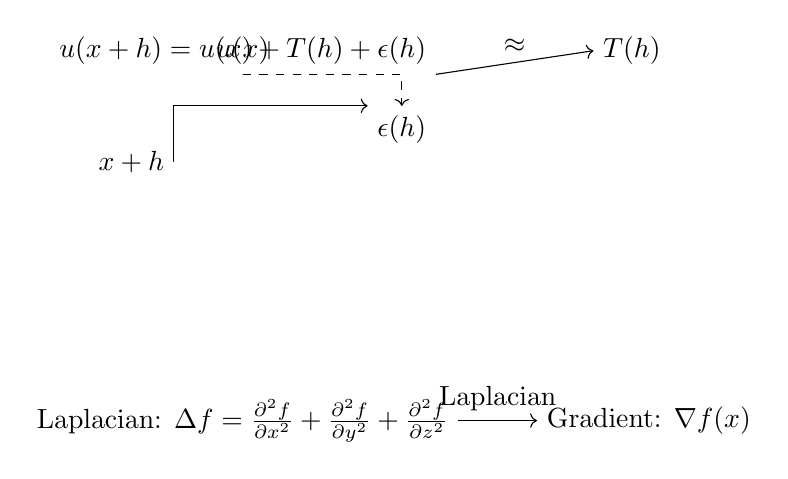
\begin{tikzpicture}[node distance=2cm]
    \node (u) at (0, 0) {\( u(x+h) = u(x) + T(h) + \epsilon(h) \)};
    \node (xh) [below left of=u] {\( x + h \)};
    \node (ux) [above right of=xh] {\( u(x) \)};
    \node (th) [right=of u] {\( T(h) \)};
    \node (epsh) [left=of th, yshift=-1cm] {\( \epsilon(h) \)};
    
    \draw[->] (u.south east) -- node[midway, above] {$\approx$} (th.west);
    \draw[->] (xh.east) |- (epsh.north west);
    \draw[dashed, ->] (ux.south) -| (epsh.north);

    \node (laplacian) [below=of u, yshift=-2cm] {Laplacian: \( \Delta f = \frac{\partial^2 f}{\partial x^2} + \frac{\partial^2 f}{\partial y^2} + \frac{\partial^2 f}{\partial z^2} \)};
    \node (grad) [right=of laplacian, xshift=-1cm] {Gradient: \( \nabla f(x) \)};
    
    \draw[->] (laplacian.east) -- node[midway, above] {$\text{Laplacian}$} (grad.west);
\end{tikzpicture}}
\end{center}
\vspace{8pt}

\begin{examplebox}[예시 1]
온도 $T(x, y)$ 가 다음과 같은 방정식에 따라 시간에 걸쳐 변화한다고 하겠습니다:
\[ \frac{\partial T}{\partial t} = k ( \nabla^2 T ) \]

여기서 $\nabla^2$는 라플라시안 연산자로, $T(x, y)$의 두 번째 도함수를 나타냅니다. 이 방정식은 열 전달 속성에 따라 온도가 주변 지역으로 퍼지는 것을 설명합니다.

\begin{itemize}
\item $\frac{\partial T}{\partial t}$는 시간 $t$ 동안 온도 $T(x, y)$의 변화율입니다.
\item $k$는 열 전달 계수로, 열이 어떻게 빠르게 퍼져나가는지를 결정합니다.
\item $\nabla^2 T = \frac{\partial^2 T}{\partial x^2} + \frac{\partial^2 T}{\partial y^2}$은 $T(x, y)$의 두 번째 도함수이며, 이는 지역적인 변화율을 나타냅니다.
\end{itemize}

따라서 이 방정식은 시간이 지남에 따라 온도가 주변 지역으로 퍼져나가는 양과 속도를 설명합니다. 예를 들어, 열 전달 계수가 높으면 온도가 더 빠르게 퍼집니다.

\#\#\#
\end{examplebox}
\vspace{4pt}

\begin{examplebox}[예시 2]
두 점 사이의 거리 $d$ 가 시간에 따라 변화한다고 하겠습니다:
\[ \frac{dd}{dt} = v(t) \]

여기서 $\frac{dd}{dt}$는 $t$ 동안 거리 $d$가 변하는 속도를 나타냅니다. 이 방정식은 물체의 운동을 설명할 때 자주 사용됩니다.

\begin{itemize}
\item $v(t)$는 시간에 따른 속도 함수입니다.
\end{itemize}
 
따라서, 이 방정식은 물체가 어떤 시점에서 어느 속도로 움직이는지를 나타냅니다. 예를 들어, 물체가 가속하는 경우 $\frac{dd}{dt}$의 값이 $t$에 따라 변할 것입니다.

\#\#\#
\end{examplebox}
\vspace{4pt}

\begin{examplebox}[예시 3]
두 점 사이의 거리 $d$와 시간 $t$ 간 관계를 다음과 같이 설명한다고 하겠습니다:
\[ \frac{\partial d^2}{\partial t^2} = a(t) \]

여기서 $\frac{\partial d^2}{\partial t^2}$는 두 점 사이의 거리가 시간에 따라 변하는 속도의 변화율을 나타냅니다. 이 방정식은 물체의 가속도를 설명할 때 자주 사용됩니다.

\begin{itemize}
\item $a(t)$는 시간에 따른 가속도 함수입니다.
\end{itemize}
 
따라서, 이 방정식은 물체가 어떤 시점에서 어느 가속도로 움직이는지를 나타냅니다. 예를 들어, 가속도가 일정하게 증가하는 경우 $\frac{\partial d^2}{\partial t^2}$의 값이 $t$에 따라 변할 것입니다.

이렇게 부분 미분 방정식은 물리학에서 매우 중요한 역할을 하며, 다양한 현상을 설명하는데 사용됩니다.
\end{examplebox}
\vspace{4pt}

\begin{exercisebox}
\textbf{1.} 기초 수준
 
 $u(x) = x^2 + 3x$ 함수가 $(0,0)$에서 미분 가능하다고 하면, 이 함수의 도함수는 무엇인가요?

2. 중급 수준

 열방정식 $\frac{\partial T}{\partial t} = \Delta f$ 에서, $T(x,y,t) = x^2 + y^2 - 3t$ 가 주어질 때, 시간에 따른 온도 변화율을 구하세요.

3. 중급 수준

 함수 $f(x,y,z)=x^2+y^2+z^2$의 라플라스 연산자를 계산해보세요.\\[4pt]

\end{exercisebox}
\vspace{4pt}

\begin{glossarybox}
\textbf{notation} --- 표기법 \\
\textbf{x for (x, y, z)} --- (x, y, z)를 x로 표기 \\
\textbf{u ( x ) for (u, v, w)} --- (u, v, w)를 u ( x )로 표기 \\
\textbf{h for (h, k, l)} --- (h, k, l)를 h로 표기 \\
\textbf{p for (p, q, r)} --- (p, q, r)를 p로 표기 \\
\textbf{T( h )} --- 벡터 h에 대한 선형 맵 T의 결과 \\
\textbf{ϵ ( h )} --- 작은 벡터 ϵ ( h ) \\
\textbf{u ( x + h ) = u ( x ) + T( h ) + ϵ ( h )} --- 함수 u가 작은 벡터 h를 더할 때의 변화식
\end{glossarybox}

\paragraph{풀이}
1. 기초 수준

 주어진 함수는 \( u(x) = x^2 + 3x \) 입니다.
 
 이 함수를 미분하면,
 \[u'(x) = 2x + 3\]
 
 따라서, $(0,0)$에서의 도함수는 $u'(0) = 3$입니다.

2. 중급 수준

 열방정식은 $\frac{\partial T}{\partial t} = \Delta f$ 입니다.
 
 주어진 함수는 \( T(x,y,t) = x^2 + y^2 - 3t \) 입니다.
 
 시간에 따른 온도 변화율을 구하기 위해 $T$를 $t$로 미분하면,
 \[\frac{\partial T}{\partial t} = -3\]

3. 중급 수준
 
 함수는 \( f(x,y,z)=x^2+y^2+z^2 \) 입니다.
 
 라플라스 연산자는 $\nabla^2$로 표현되며, 이는 $f$에 대한 두 번째 도함수의 합입니다. 즉,
 \[\nabla^2 f = \frac{\partial^2 f}{\partial x^2} + \frac{\partial^2 f}{\partial y^2} + \frac{\partial^2 f}{\partial z^2}\]
 
 $f(x,y,z)$에 대해 각각 미분하면,
 \[\nabla^2 f = 2 + 2 + 2 = 6\]



% ═══ Section 5.5: Integration ═══
\section{적분}
\label{sec:5-5}

III. 몇 가지 기본 수학적 개념

f(x−h)−f(x) : f 함수에서 x 에서의 함숫값과 근처 지점인 x+h 및 x-h 에 대한 평균값 사이의 차입니다. 다시 말해, 이차 도함수는 우리가 원하는 개념을 나타냅니다—x 에서의 함숫값과 주변 지역의 평균값 간 비교 입니다. 만약 f 가 선형 함수라면, f(x−h) 와 f(x+h) 의 평균은 f(x)와 같다는 것이 알려져 있죠.이는 선형 함수의 제일 도함수가 영임으로부터 유래된 친숙한 사실과 부합됩니다. 첫 번째 도함수를 정의할 때 마찬가지로 그 크기를 자동적으로 작게 하도록 f(x+h)-f(x) 를 h 로 나누었듯이 두번 미분 또한 적절히 h² 로 나눌 필요가 있습니다. (첫 번째 도함수는 직선적인 근사치와 관련되어 있으며, 두 번째 도함수는 제 2 계근사치와 관련되어 있는데, 함수 f 는 변화량 x 인 곳에서 가장 좋은 제 2 계근사치는 
f(x+h)≈f(x)+hf′(x)+1/2h²f″(x),라고 합니다.)

위와 같은 생각을 추적하고 세 가지 변수 함수인 경우 Δf 값이 (x,y,z) 에서의 f 의 함숫값이 주변 지점들의 평균값들과 어떻게 비교되는지를 보여줍니다. 여기에 특별한 것은 없으며 - 아이디어들은 모든 변수 개수에 일반화될 수 있습니다. 열방정식에서는 매개변수 κ 가 논해야 할 내용입니다. 이것은 물질의 전기전도율을 나타냅니다. 만약 κ 가 작다면 재료가 열을 잘 전하지 않아서 ΔT 가 온도 변화 속도에 미치는 영향력이 적어집니다; 크기를 가져야 한다면 더 많은 효과를 얻고 그렇지 않습니다. 매우 중요한 또 다른 식은 라플라스 방정식 입니다: Δf=0 . 직관적으로 말하면, 이것이 함수 f 에 대해 그것의 x , y , z 점에서의 함숫값이 즉각적인 인접 위치의 평균값과 항상 같다고 합니다.만약 f 는 단 하나의 변수인 x 로 구성된 함수라면, 이것은 f 의 제 2 도함수가 0 임을 의미하며 결과로 a*x+b 형태라는 결론으로 나옵니다. 하지만 두 가지 이상의 변수에서는 함수가 더 유연하게 행동할 수 있으며 일부 방향에서는 접선 위이고 다른 방향에서는 아래쪽일 수 있으므로 다양한 경계 조건들을 임명하여 (특정 지역들의 경계에서 f 가 취하는 값들) 훨씬 광범위하고 매혹적이며 해결책들이 많습니다.

세 번째 기본 공식은 파동방정식입니다. 한 차원 표현형으로서 A 와 B 사이에 연결되어 있는 진동 현실의 운동을 설명합니다. 시간 t 에서 거리 x 만큼 높이의 현의 높이를 h(x,t) 라고 적으면 다음과 같은 식입니다:
1/v²∂²h /∂t² = ∂²h /∂x². $v^2$ 를 무시하면 우변은 지점 x 에 위치한 줄기 부분의 가속도(직진성)를 나타냅니다. 그러한 물체는 어떤힘으로 작용하도록 합니다? 이제 string 의 절반만 완전히 직선 상태라고 생각해 보세요.그러면 x 의 왼편줄기에 걸리는 압력이 오른 편줄기를 정확히 상쇄하기 때문에 순응력은 영됩니다. 따라서 다시 한 번 중요한 것은 변수 x 와 주변 두 점 간 비교가 되어야 한다는 것입니다; 선물이 접선 위쪽에 있다면 올라오는 힘이 생길 것이며 아래로 있으면 내려오는 힘이 발생할 것이다. 바로 그것 때문인지 여섯 번째 도함수가 반복적으로 등장하는 것처럼 느껴질 수 있습니다. 두번째 미분에서 기여되는 힘의 크기는 줄자리와 치밀하게 연결된 요소들에 달려있습니다, 그리고 거기에서 일정 값이 들어옵니다. h 는 x 모두 길이의 단위이며, $v^2$ 은 (거리/시간)\^{}2 로 표현되므로, v 는 파동 전파 속도라는 것을 의미합니다.

유사한 고찰을 통해 세 차원 파동방정식이 얻어집니다: 
1 /v²∂²h /∂t² = ∂²h /∂x²+∂²h /∂y²+∂²h /∂z², 또는 간단히 말하면 : 
1/ v²∂²h /∂t²=Δh 라고 표현할 수 있습니다. 이를 더욱 축약하여 다음과 같이 나타낼 수 있습니다.: □²h=0 , 여기서 □²h 는 Δh - 1/v²∂²h /∂t² 를 의미하는 약자입니다. 작업은 d'Alembert(VI.20) 에 따라 제시되어 처음으로 파동 방정식을 공식화했던 사람인 d’alembert 입니다.

5.5 통합 적분

차량이 한 분 동안 길고 직선적인 도로를 주행한다고 가정하고 시작 위치와 그 시간 내내 속도에 대한 정보가 제공된다면 자동차의 이동 거리를 계산하는 방법은 무엇일까요? 만약 차량이 온전히 같은 속력으로 운전했다면 문제는 매우 간단합니다 — 예를 들어, 속도가 마일당 삼십마일이고 t 는 초라고 하겠습니다. \[v(t) = \frac{s}{1}\] \[\int_{0}^{60} v(t) dt \] \[d= \int_{0}^{60} v(t) dt \] $\text { } d=\left[\right]_{0}^{60}$ 한 시간이면 여섯십을 나누어 보니 반 마일 정도 이동했다는 것을 알 수 있지만, 문제가 더욱 흥미롭게 변하는 것은 속력이 다르다면입니다. 그러므로 정확한 값을 주기보다는 다음과 같은 기술로 근사치를 구할 수 있습니다. 우선 자동차의 각 분 단위에서 시점별 속력을 기록합니다. 그리고 이들 중 하나에 대해 해당 순간 동안 속력이 처음부터 계속 유지된 경우 차량이 얼마나 진행되었는지를 간단하게 계산합니다. 마침내 모든 거리를 합칩니다. 한초라는 기준은 매우 작으므로 어떤 단위 안에서는 속력이 크게 바뀌지 않아 따라서 이 절차는 상대적으로 정밀한 결과를 제공합니다. 게다가 만약 당신께서 얻고 있는 정밀성에 불만족한다면 하루 종일에보다 짧은 간격들을 사용하여 그것을 개선할 수 있습니다.

처음 미적분 과정을 완료하신 후에는 전혀 다른 방식으로 비슷한 문제를 해결해 온 경험이 있겠죠? 일반적인 질문에는 시간 t 에서 속도 공식인 at + u 와 같이 명시되어 있으며, 차량이 이동하는 거리 계산하기 위해 "적분"하면 1/2$at^2$+ut 와 같은 함수로 표현됩니다. 여기서는 적분이 도함수의 반대로 생각되며 f(t) 가 주어진 함수일 때 g'(t)=f(t) 를 충족하는 함수 g 를 찾는 것을 의미합니다. 그것은 논리가 맞습니다.왜냐하면 g(t) 는 이동거리고 f(t) 는 속도라면 f(t) 는 실제로 g(t)' 의 변화율입니다. 그러나 역미분법은 적분의 정의가 아닙니다. 다음과 같은 질문을 고려해서 이것을 알아보세요: $e^{-$t\^{}2$}$ 로 나타내지는 시각에서 얼마나 진행되었습니까? 다항식 , 지수함수, 로그 및 삼각함수 등 기본적으로 구성된 함수에 대한 것이라고 합니다.)라는 미분값으로 얻음; 하지만 문제 자체는 합리성이 있고 확실한 해결책이 있습니다.(Φ(t) 라는 함수가 존재한다는 이야기를 들었을 수도 있는데 Φ(t
√
2 ) / √2 e − $t^{2}$ 에 대해서 미분되어 나오는데에도 불구하고 어렵게 남겨지기 때문에 φ (t) 은 절대적정해와 같다고 할 수 없습니다).

위처럼 반대로 생각할 때 도움이 되도록 복잡하게 근사치를 사용해야 하는 상황에서는 적분을 정의하는 방법이 있어야 합니다. 중세 후반기에 리만 [VI.49] 가 제시했던 방안들이 있다면 그러한 형태로 공식적인 정의입니다. Riemann 의 주요 아이디어를 보여주며 또한 미적분과 마찬가지로 여러 변수 이상의 함수에 유용하게 활용될 수 있는 과정임을 알아보려면 다른 물리학적 문제를 살펴봅니다. 혼합되지 않은 돌덩이의 무리를 가지고 있으며, 이것에서밀도를 계산하려고합니다. 그리고 더불어 치밀하지 못하며 심각히 일관성 없는 상태일 가능성이 높습니다.

리 emann 접근법은 다음과 같습니다. 첫째, 주변 영역을 직육형으로 감싸봅니다. 각 점 $(x, y, z)$ 에 해당되는 직육형 내에는 연속적으로 변화하는 값 $d(x, y, z)$가 존재하며 ($x$, $y$, $z$) 와 같은 형태입니다). 두 번째로, 직육형을 작은 직육형으로 분할합니다. 세번째로, 각 소직육형 내에서는 가장 작게 나타나는 값과 가장 크게 나타나는 값을 찾으십시오 (외부 또는 구멍 안의 지점들은 항상 0 이라고 간주합니다). C 라는 하나의 소직육형에 최솟값 a 와 최댓값 b 가 있고 V 는 C 의 부피일 때, C 내 모든 돌들의 질량은 abV 사이에 있습니다. 네 번째로, 얻어진 모든 abv 들을 더해줍니다. M1 과 M2 라고 하는 이 합계인 경우 전체적인 덩이의 무게는 M1 과 M2 사이에서 존재합니다. 마지막으로 미세한 분할 조건까지 반복하면 M1 과 M2 를 계산하여 결과적으로 절정적이고 정확하게 근사치 접근법을 제공받습니다.

마찬가지로 자동차 문제도 동일한 방식으로 처리됩니다: 시간 간격을 매우 작게 설정하고 해당 주간 속력의 최저최대값을 살펴봅니다. 각 간격에는 'a' 와 'b' 라는 두 가지 수열이 있으며 차량 이동 거리가 적어도 "a" 만큼 그리고 많아서 "b" 로 표현될 수 있습니다.

두 개의 예제 모두 함수(밀도/속도) 에 대해 집합 (구체 또는 한분의 시점 ) 을 사용했으며 특별히 말해서 그 기능의 총 양을 파악하려했습니다. 우리는 소부위들로 구성된 세트들을 나누고 각 부위에 대한 단순 계산을 통해 위와 아래쪽으로 추측하는 방법을 활용함으로써 이것을 달성했습니다.

이는 리만 적분 으로 알려진 과정입니다. 다음은 일반적인 표현이며, S 가 집합이고 f 는 함수라면 S 에서 f 의 총 합 즉 적분 은 $\int_S f(x) dx$ 입니다. 여기에서 x 는 S 의 대표적 요소를 의미합니다.


\vspace{8pt}
{\large\textbf{\textsf{심층 해설 (Deep Research)}}}
\vspace{4pt}


\begin{researchbox}[라플라스 방정식 (Laplace equation)]
라플라스 방정식은 공간에서의 변화를 균형 있게 유지하는 함수를 찾는 방정식으로, 수학과 물리학에서 중요한 역할을 합니다. 이 방정식은 전기장, 중력장, 열 분포 등 다양한 현상을 설명하는 데 사용되며, 함수의 값이 주변 평균과 같아야 한다는 조건을 수학적으로 표현한 것입니다. 이 섹션에서 언급된 이차 미분의 개념과 연결되면, 라플라스 방정식은 다차원 공간에서의 '균형 상태'를 나타내는 비유로 이해할 수 있습니다. $ \nabla^2 f = 0 $은 함수 $ f $가 균일하게 퍼져 있어야 한다는 의미를 담고 있습니다.
\vspace{2pt}
{\scriptsize \textit{출처: Wikipedia --- Laplace's equation}}
\end{researchbox}
\vspace{4pt}


\begin{researchbox}[열 방정식 (Heat equation)]
열이 물체 안에서 어떻게 퍼지는지를 설명하는 수학 방정식으로, 시간이 지남에 따라 온도가 균일해지는 과정을 모델링합니다. 이 방정식은 물리학과 수학에서 열 전달, 확산 현상 등을 이해하는 데 핵심적인 역할을 하며, 특히 편미분 방정식의 기초를 이루는 중요한 개념입니다. 이 섹션에서 설명된 이차 미분의 개념은 열 방정식이 공간에서의 평균 온도와의 차이를 설명하는 데 직접적으로 연결됩니다.
\vspace{2pt}
{\scriptsize \textit{출처: Wikipedia --- Heat equation}}
\end{researchbox}
\vspace{4pt}


\begin{researchbox}[라플라시안 (Laplacian)]
라플라시안은 함수의 값을 주변 평균과 비교해 그 곡률을 측정하는 미분 연산자로, $ \Delta f = \nabla \cdot \nabla f $ 또는 $ \nabla^2 f $로 표현됩니다. 물리학에서 중력장, 전기장, 열 전달 등 다양한 현상을 설명하는 데 핵심적인 역할을 하며, 특히 진공 영역의 중력 잠재 에너지를 나타내는 조화 함수와 관련이 깊습니다. 이 섹션에서 두 번째 미분이 특정 점의 값과 주변 평균의 차이를 설명하는 것처럼, 라플라시안은 다차원 공간에서 이 차이를 일반화한 개념입니다.
\vspace{2pt}
{\scriptsize \textit{출처: Wikipedia --- Laplace operator}}
\end{researchbox}
\vspace{4pt}


\begin{researchbox}[이차 도함수 (Second derivative)]
두 번째 도함수는 변화의 속도가 어떻게 변하는지를 나타내는 개념입니다. 예를 들어, 물체의 위치에 대한 시간에 대한 두 번째 도함수는 가속도로, 속도가 얼마나 빨라지는지를 설명합니다. 이는 물리학에서 운동 분석이나 수학에서 곡선의 볼록성을 판단하는 데 중요합니다. 이 섹션에서는 두 번째 도함수가 특정 지점의 값과 주변 평균 값을 비교하는 방식으로 정의됨을 설명합니다. 첫 번째 도함수는 순간적인 변화를, 두 번째 도함수는 그 변화가 어떻게 변하는지를 보여주는 것이라 비유할 수 있습니다.
\vspace{2pt}
{\scriptsize \textit{출처: Wikipedia --- Second derivative}}
\end{researchbox}
\vspace{4pt}


\begin{researchbox}[이차 근사 (Quadratic approximation)]
이차 근사법은 함수를 이차 다항식으로 근사하는 방법으로, 곡선의 모양을 더 정확하게 표현할 수 있게 해줍니다. 이 방법은 수학에서 복잡한 함수를 간단한 식으로 대체할 때 유용하며, 물리학이나 공학에서도 계산을 쉽게 해주는 데 사용됩니다. 이 섹션에서 두 번째 도함수와 주변 평균값의 관계를 설명한 것처럼, 이차 근사법은 함수의 곡률을 반영하는 데 중요한 역할을 합니다. $f(x)$를 $f(x) \approx f(a) + f'(a)(x-a) + \frac{f''(a)}{2}(x-a)^2$로 표현할 수 있으며, 이는 함수의 변곡점을 이해하는 데 도움이 됩니다.
\vspace{2pt}
{\scriptsize \textit{출처: Wikipedia --- Taylor's theorem}}
\end{researchbox}
\vspace{4pt}


\begin{researchbox}[전도도 (Conductivity)]
열전도율은 물질이 열을 얼마나 잘 전달하는지를 나타내는 값으로, 수학적으로 $ k $, $ \lambda $, $ \kappa $로 표기하며 단위는 W·m⁻¹·K⁻¹입니다. 고전도율 물질은 열이 빠르게 흐르는 열교환기로 사용되고, 저전도율 물질은 단열재로 활용됩니다. 이 개념은 수학적 정의 섹션에서 열 흐름을 설명하는 미분 방정식 $ \mathbf{q} = -k\nabla T $와 연결되어, 함수의 변화율을 이해하는 데 도움을 줍니다.
\vspace{2pt}
{\scriptsize \textit{출처: Wikipedia --- Thermal conductivity and resistivity}}
\end{researchbox}
\vspace{4pt}


\begin{verificationbox}
\textbf{종합 점수: 58/100 (주의)} \\[2pt]
{\small 수식 100 \quad 의미 21 (6건) \quad 논리 73 (3건) \quad 검증 20 (4건)}
\end{verificationbox}
\vspace{4pt}


\begin{summarybox}
이 글에서는 함수와 그 도함수, 둘러싸는 지역 평균값 사이의 관계를 설명하며, 이 개념을 통해 선형성과 변화량에 대한 이해를 깊게 합니다. 또한, 두 번째 도함수와 라플라스 방정식은 함수가 어떤 위치에서 가장 잘 근사되는지 알려주는 중요한 공식입니다. 마지막으로, 파동방정식은 시간과 거리의 관계를 설명하며, 이는 물질의 전기전도율이나 진동 현상을 이해하는 데 도움이 됩니다. 통합 적분을 통해 변화량에 대한 정확한 값들을 계산할 수 있는 방법도 소개됩니다.
\end{summarybox}
\vspace{8pt}

\begin{center}
\resizebox{\textwidth}{!}{\begin{tikzpicture}[node distance=1cm, auto]
    \node (f) {f(x)};
    \node[right of=f] (h_plus_f) {$f(x+h)$};
    \node[below right of=h_plus_f] (avg_val) {\textcolor{black}{$\frac{f(x-h)+f(x+h)}{2}$}};
    
    \draw[-latex, thick] (f.south) -- node[midway, below] {x} ++(0,-1);
    \draw[-latex, thick] (h_plus_f.east) -- node[midway, right] {$x+h$} ++(1,0);
    \draw[-latex, thick] (avg_val.west) -- node[midway, left] {$f(x-h)$} ++(-1,0);
    
    \node[below of=avg_val, yshift=-2cm] (second_derivative) {두 번째 도함수};
    \draw[dashed, -latex, thick] (second_derivative.west) -- node[midway, below left] {$f(x+h)\approx f(x)+hf'(x)+\frac{1}{2}h^2f''(x)$} ++(-3,-0.5);
    
    \node[below of=second_derivative, yshift=-4cm] (laplacian) {라플라스 방정식};
    \draw[dashed, -latex, thick] (laplacian.west) -- node[midway, below left] {$\Delta f = 0$} ++(-3,-1);
    
    \node[below of=laplacian, yshift=-6cm] (wave_equation_2d) {두 차원 파동방정식};
    \draw[dashed, -latex, thick] (wave_equation_2d.west) -- node[midway, below left] {$\frac{1}{v^2}\partial_{tt}h = \partial_{xx}h$} ++(-3,-0.5);
    
    \node[below of=wave_equation_2d, yshift=-8cm] (wave_equation_3d) {세 차원 파동방정식};
    \draw[dashed, -latex, thick] (wave_equation_3d.west) -- node[midway, below left] {$\frac{1}{v^2}\partial_{tt}h = \partial_{xx}h + \partial_{yy}h + \partial_{zz}h$} ++(-3,-0.5);
    \draw[dashed, -latex, thick] (wave_equation_3d.west) -- node[midway, below left] {$\Box^2 h = 0$} ++(-3,-1);
    
    \node[below of=wave_equation_3d, yshift=-10cm] (summary) {세 가지 기본 공식};
    \draw[dashed, -latex, thick] (summary.west) -- node[midway, below left] {$f(x+h)-f(x)$: x에서의 함숫값과 근처 지점들의 평균값 사이의 차} ++(-3,-0.5);
\end{tikzpicture}}
\end{center}
\vspace{8pt}

\begin{examplebox}[예시 1]
주행하는 차량의 속도는 시간에 따라 변동됩니다. 예를 들어, t=0 초에서 시작하여 t=60 초까지의 속도가 다음과 같이 주어졌다고 하겠습니다.
\[ v(t) = \begin{cases} 
30 & (t ≤ 20) \\
45 & (20 < t ≤ 40) \\
30 & (40 < t ≤ 60)
\end{cases} \]
이 경우, 자동차의 이동 거리를 계산하려면 각 구간별로 적분을 수행해야 합니다.
\[ d = \int_{0}^{20} v(t) dt + \int_{20}^{40} v(t) dt + \int_{40}^{60} v(t) dt \]
각 구간의 정적분 결과를 더하면 총 이동 거리가 계산됩니다.
\end{examplebox}
\vspace{4pt}

\begin{examplebox}[예시 2]
두 점 사이의 물체 움직임을 나타내는 함수 f(x) 가 주어졌다고 하겠습니다. 예를 들어, x=0 에서 시작하여 x=5 까지의 위치 변화를 보여주는 함수가 다음과 같습니다.
\[ f(x) = \begin{cases} 
x^2 & (0 ≤ x < 3) \\
4 + 2(x-3) & (3 ≤ x ≤ 5)
\end{cases} \]
이 경우, 물체의 이동 거리를 계산하려면 각 구간별로 적분을 수행해야 합니다.
\[ d = \int_{0}^{3} f'(x) dx + \int_{3}^{5} f'(x) dx \]
각 구간의 정적분 결과를 더하면 총 이동 거리가 계산됩니다.
\end{examplebox}
\vspace{4pt}

\begin{examplebox}[예시 3]
두 점 사이에 물체 움직임을 나타내는 함수 f(x,t) 가 주어졌다고 하겠습니다. 예를 들어, t=0 초에서 시작하여 t=60 초까지의 위치 변화를 보여주는 함수가 다음과 같습니다.
\[ f(x,t) = \begin{cases} 
x^2 & (t ≤ 30) \\
4 + 2(t-30) & (30 < t ≤ 60)
\end{cases} \]
이 경우, 물체의 이동 거리를 계산하려면 각 구간별로 적분을 수행해야 합니다.
\[ d = \int_{0}^{30} f'(x,t) dt + \int_{30}^{60} f'(x,t) dt \]
각 구간의 정적분 결과를 더하면 총 이동 거리가 계산됩니다.
\end{examplebox}
\vspace{4pt}

\begin{exercisebox}
\textbf{1.} 문제 1 (기초):
함수 f(x) = $x^2$ + 3x + 5 의 두 번째 도함수가 무엇인가요?

문제 2 (중급):
다음 함수에 대해 라플라스 방정식을 적용하여 Δf 값을 구해보세요. 
f(x,y,z) = $x$y\^{}{2}$z$\^{}3\\[4pt]

\end{exercisebox}
\vspace{4pt}

\begin{glossarybox}
\textbf{derivative} --- 도함수 (변화율) \\
\textbf{second derivative} --- 이차도함수 (곡률) \\
\textbf{linear function} --- 선형 함수 \\
\textbf{quadratic approximation} --- 제곱근 근사 \\
\textbf{Laplace equation} --- 라플라스 방정식 (평균값과 일치)
\end{glossarybox}

\paragraph{풀이}
1. 문제 1 (기초):

함수 f(x) = $x^2$ + 3x + 5 의 두 번째 도함수가 무엇인가요?

풀이: 
\begin{itemize}
\item 첫 번째 도함수를 구합니다.
\end{itemize}
\[ f'(x) = \frac{d}{dx}(x^2 + 3x + 5) = 2x + 3 \]
\begin{itemize}
\item 두 번째 도함수를 구합니다.
\end{itemize}
\[ f''(x) = \frac{d}{dx}(2x + 3) = 2 \]

따라서, 함수 \(f(x)\)의 두 번째 도함수는 \(2\)입니다.

---

2. 문제 2 (중급):

다음 함수에 대해 라플라스 방정식을 적용하여 Δf 값을 구해보세요.
\[ f(x,y,z) = xy^2z^3 \]

풀이: 
\begin{itemize}
\item 라플라스 연산자 \(Δ\)는 다음과 같습니다:
\end{itemize}
\[ Δ = \frac{\partial^2}{\partial x^2} + \frac{\partial^2}{\partial y^2} + \frac{\partial^2}{\partial z^2} \]

\begin{itemize}
\item 각 변수에 대한 두 번째 편미분을 구합니다.
\end{itemize}
\[ \frac{\partial f}{\partial x} = y^2z^3, \quad \frac{\partial^2 f}{\partial x^2} = 0 \]
\[ \frac{\partial f}{\partial y} = 2xyz^3, \quad \frac{\partial^2 f}{\partial y^2} = 2xz^3 \]
\[ \frac{\partial f}{\partial z} = 3xy^2z^2, \quad \frac{\partial^2 f}{\partial z^2} = 6xy^2z \]

\begin{itemize}
\item 라플라스 연산자를 적용합니다.
\end{itemize}
\[ Δf(x,y,z) = \frac{\partial^2 f}{\partial x^2} + \frac{\partial^2 f}{\partial y^2} + \frac{\partial^2 f}{\partial z^2} \]
\[ Δf(x,y,z) = 0 + 2xz^3 + 6xy^2z \]

따라서, 함수 \(f(x,y,z)\)의 라플라스 값은 \(2xz^3 + 6xy^2z\)입니다.



% ═══ Section 5.6: Holomorphic Functions ═══
\section{정칙 함수}
\label{sec:5-6}

I.3. 기본적인 수학적 개념들

$(x, y, z)$와 같은 벡터 표현도 $Sf( x ) dx$처럼 사용할 수 있으나, 종종 일반적인 "x" 가 실수보다 벡터를 나타내는지 독자가 추론하도록 둡니다. 적분과 미분 방정식의 차별성에 신경 쓰였지만, 계산 기본 정리라고 알려진 명제에서 두 과정이 특정 연속 조건을 만족하는 함수일 때 동일한 결과를 가져온다고 주장한다. 따라서 통상적으로 적분을 미분의 반대로 간주해도 좋습니다. 더 자세히 말하면, 연속인 함수 f 를 가지고 다음으로 F(x)를 정의 한다면 :

\[F(x)= \int_a^{x}f(t) dt \]

어떤 a 에 대해, F 는 미분 가능하며 $F'(x) = f(x)$. 다시 말해서 지연된 연속함수를 적분하고 다시 미분하면 시작점으로 돌아옵니다. 다른 관점에서는, 연속인 도함수 f 와 a < x 라면:

\[\int_a^x f(t)dt= F(x)-F(a)\]
이는 “미분하여 얻은 값” 을 다시 한번 적분하면 원래 형태가 되기 때문입니다. 실제로는 임의적인 상수 a 를 선택해야 하므로 구하게 된 것은 일관되지만 F(a) 로부터 제외되는 것입니다.

위에서 설명한 내용은 모든 함수에 해당하지 않으며 특정 조건들을 만족시켜야 하는 경우처럼 다르거나 예측 불가능한 결과들이 발생하기도 합니다. 위에서 언급했던 Heaviside 단계 함수 H(x)와 같은 예들은 주목할 필요가 있습니다.

\[H(x)= \begin{cases}
0 & (x<0)\\
1 & (x\geq 0)
\end{cases}\]

이것은 x = 0 에서 점프를 가지고 불연속적이며 따라서 일반적으로 정리된 미분 방식으로 계산될 수 없습니다. J(x) 는 다음과 같습니다 : \[J(x)=\begin{cases}
0 & (x < 0)\\
x & (x \geq 0)
\end{cases}\]

그리고 거의 모든 x 에 대해 $J'(x) = H(x)$ 입니다 .그러나 gradient of J 가 x=0 에서 갑자기 변하므로, 이는 미분 가능하지 않으며 $J'(0) = H(0) = 1$ 라고 말할 수 없습니다.

5.6 복소함수

복잡 분석은 복소 수를 입력으로 받고 복소 수를 출력하는 미분 가능 함수 연구하며, 수학에서 가장 귀중하게 여겨지는 분야 중 하나입니다. 이러한 종류의 함수는 "정칙"이라고 합니다. 처음에는 이와 같은 함수가 특별해 보일지도 모르겠지만, 실변수 함수에 대한 도함수 정의와 동일하기 때문입니다. 만약 f 가 함수라면 복소수 z 에서의 도함수 f’(z) 는 h 를 0 으로 접근시키며 식 ((f(z+h)-f(z))/h ) 의 한계로 정의됩니다. 하지만 우리가 위 정의를 조금 다른 관점에서 살펴보게 되면 (5.3 절에서 본 방법과 유사), 복소 함수가 미분될 것이라는 것은 결코 간단하지 않습니다. 해당 절에서는 미분이 선형 근사 의미임을 기억하십시오. 복소 함수의 경우 g(w) = λw + μ 형태의 함수로 근사하고자 하는 것을 의미합니다. λ 와 μ 는 모두 복소수 입니다.(g(w) = f(z)+f'(z)(w-z) 로서 z 에 인접한 근사값은 주어져 있으며 ,이는 λ=f'(z) 그리고 μ= f(z)-zf'(z) 라는 결과를 제공합니다.)

우리가 이 상황을 기하적으로 생각해 보겠습니다. 만약 λ ≠ 0 이라면, λ로 인한 효과는 z 를 일부 요인 r 로 확장하고 θ 각도 만큼 회전시키는 것입니다. 따라서 평면 변환 중 일반적인 선형 변환들처럼 반영이나 스트레칭 등 많은 것이 제외됩니다. λ 를 지정하기 위해서는 두 개의 실수 값이 필요합니다(a+bi 또는 r$e^{iθ }$ 형태로 표현할 수 있기 때문입니다), 하지만 일반적인 평면 선형변환을 정의하려면 네 개가 필요합니다 (4 절 참조). 자유도 차원 감소는 코시-리 emann 방정식으로 나타납니다. f(z) 대신 u(x + iy) + iv(x + iy) 와 같이 쓰고, x 와 y 는 복소수 z 의 실수 부분 및 허상 부분이며 ,u(x + iy) 과 v(x + iy) 는 f(x + iy) 의 실수 부분 및 허상 부분임을 기억하십시오. 그러므로 z 근처에서 f 에 대한 선형근사에는 다음과 같은 행렬이 있습니다:

⎛
⎜⎜⎜⎝∂u/∂x ∂u/∂y
∂v/∂x ∂v/∂y⎞⎟⎟⎠

팽창 및 회전의 행렬은 항상 다음 형태를 가집니다.: $\begin{pmatrix}a & b \\ -b & a\end{pmatrix}$ , 이로부터 우리는 $\frac{\partial u}{\partial x}=\frac{\partial v}{\partial y}$ 와 $\frac{\partial u}{\partial y}=-\frac{\partial v}{\partial x}$ 를 유도할 수 있습니다. 이것들이 코시-리만 방정식입니다. 이러한 방정식들의 한 결과는 $\frac{\partial^2u}{\partial x^2}+\frac{\partial^2u}{\partial y^2}= \frac{\partial^2v}{\partial x\partial y}-\frac{\partial^2v}{\partial y\partial x}=0$ 입니다.(혼합 편미분 도함수의 대칭성이 필요한 조건을 만족하는지 명확하지 않지만, f 가 정칙 함수일 때 그렇게 합니다.) 따라서 $u$ 는 라플라스 방정식(5 장 4 절에서 논의됨) 을 만족합니다. 비슷한 주장으로 $v$ 또한 한다고 할 수 있습니다.

이런 사실들은 복소 미분 가능성이 실제 미분 가능성보다 강력하다는 것을 시사하며, 정칙 함수에는 놀랍도록 매혹적인 성질들을 가진다고 기대하게 하며 우리를 설득한다. 본 절 나머지를 통해 진행되는 것처럼, 그들에 의해 가지는 일부 눈에 띄는 특징들을 살펴보겠습니다.
첫 번째는 (직전 부문에서 다룬) 미적분학의 기본 이론과 관련되어 있습니다. F 가 정칙 함수이고 다음 정보들이 제공된다면


\vspace{8pt}
{\large\textbf{\textsf{심층 해설 (Deep Research)}}}
\vspace{4pt}


\begin{researchbox}[정칙 함수 (Holomorphic Functions)]
복소수 변수를 사용하는 함수 중, 복소수 평면의 각 점 주변에서 미분 가능한 함수를 훌로모르픽 함수라고 합니다. 이 함수는 무한히 미분 가능하고, 테일러 급수로 표현될 수 있어 매우 매끄럽습니다. 복소 해석학의 핵심 개념으로, 물리학이나 공학에서 중요한 역할을 하며, 이 섹션에서는 수학의 기초 정의를 다루고 있으므로 훌로모르픽 함수는 핵심적인 내용으로 등장합니다.
\vspace{2pt}
{\scriptsize \textit{출처: Wikipedia --- Holomorphic function}}
\end{researchbox}
\vspace{4pt}


\begin{researchbox}[복소 해석학 (Complex Analysis)]
복소 해석학은 복소수 변수를 사용하는 함수를 연구하는 수학의 한 분야로, 실수 함수와 달리 복소수 함수는 자연스럽게 무한 번 미분 가능하고 테일러 급수로 표현될 수 있다는 특징이 있습니다. 이 분야는 물리학, 공학, 수학의 여러 분야에서 중요한 도구로 사용되며, 유체역학, 양자역학, 전기공학 등에 응용됩니다. 이 섹션에서 다루는 적분과 미분의 관계는 복소 해석학의 결과를 통해 더 깊이 이해할 수 있습니다.
\vspace{2pt}
{\scriptsize \textit{출처: Wikipedia --- Complex analysis}}
\end{researchbox}
\vspace{4pt}


\begin{researchbox}[미적분학의 기본 정리 (Fundamental Theorem of Calculus)]
미적분학의 기본 정리는 미분과 적분이 서로 역연산임을 알려주는 정리로, 함수의 기울기와 면적을 연결해 줍니다. 이 정리는 정적분을 계산할 때 미분 가능하면 적분을 쉽게 해주는 방법을 제공해, 수학, 물리, 공학 등 다양한 분야에서 활용됩니다. 이 섹션에서는 적분과 역도함수를 구분했지만, 이 정리는 두 개념이 실제로 같은 결과를 주는 것을 설명합니다. 예를 들어, 속도를 적분하면 이동 거리가 되고, 이동 거리를 미분하면 다시 속도가 되는 것처럼, 두 연산은 서로 반대되는 역할을 하지만 결과적으로 연결됩니다.
\vspace{2pt}
{\scriptsize \textit{출처: Wikipedia --- Fundamental theorem of calculus}}
\end{researchbox}
\vspace{4pt}


\begin{researchbox}[헤비사이드 계단 함수 (Heaviside Step Function)]
히비시드 계단 함수는 음수 입력값에서는 0, 양수에서는 1 을 주는 함수로, 전기 신호나 물리 현상에서 갑작스럽게 변화하는 상황을 모델링하는 데 사용됩니다. 이 함수는 미분 방정식을 푸는 데 사용되며, 특정 시간에 작동을 시작하고 계속 유지하는 신호를 나타내는 데 유용합니다. 이 섹션에서는 수학의 기본 개념을 다루고 있으며, 히비시드 계단 함수는 이에 해당하는 계단 함수의 예시로, 다양한 수학적 문제에서 사용됩니다.
\vspace{2pt}
{\scriptsize \textit{출처: Wikipedia --- Heaviside step function}}
\end{researchbox}
\vspace{4pt}


\begin{researchbox}[미분 가능한 함수 (Differentiable Functions)]
미분 가능한 함수는 그림처럼 매끄럽고, 꺾인 부분이나 뾰족한 모서리가 없어 각 점에서 기울기를 정의할 수 있는 함수입니다. 이 개념은 물리학이나 경제학에서 변화를 정확히 설명할 때 필수적이며, 계산이 용이한 매끄러운 곡선을 다루는 데 사용됩니다. 이 섹션에서는 미적분학의 기초 개념을 설명하고 있으므로, 미분 가능성이 적분과의 관계를 이해하는 데 중요한 역할을 합니다.
\vspace{2pt}
{\scriptsize \textit{출처: Wikipedia --- Differentiable function}}
\end{researchbox}
\vspace{4pt}


\begin{researchbox}[연속의 성질 (Continuity Properties)]
연속 함수는 입력값이 조금만 변해도 출력값이 크게 달라지지 않는 함수로, 그래프상에서 갈라짐이나 뚝 끊김이 없는 부드러운 곡선을 만들 수 있습니다. 이 개념은 미적분학에서 적분과 미분을 연결하는 데 핵심적이며, 특히 적분과 역도함수의 관계를 설명하는 기본 정리에서 중요한 역할을 합니다. 이 섹션에서는 연속성 덕분에 적분과 미분이 서로 관련되어 있음을 보여주는 정리가 등장하므로, 연속성은 이들 개념을 이해하는 데 필수적입니다.
\vspace{2pt}
{\scriptsize \textit{출처: Wikipedia --- Continuous function}}
\end{researchbox}
\vspace{4pt}


\begin{verificationbox}
\textbf{종합 점수: 67/100 (주의)} \\[2pt]
{\small 수식 100 \quad 의미 19 (6건) \quad 논리 90 (2건) \quad 검증 60 (2건)}
\end{verificationbox}
\vspace{4pt}


\begin{summarybox}
정규함수와 복소함수에 대한 핵심 개념을 간략히 요약하면 다음과 같습니다:

1. 정규함수는 연속적인 함수를 적분하고 다시 미분할 때 원래의 함수로 돌아오는 특성을 가집니다.

2. Heaviside 단계 함수 H(x)와 같은 예시들은 일반적 미분 방식으로 계산될 수 없는 불연속적인 함수입니다.

3. 복소함수는 실변수 함수에 대한 도함수 정의와 동일하게, 그 근사값을 통해 미분 가능성을 판단할 수 있습니다.

4. 코시-리만 방정식은 복소함수가 미분 가능한 조건으로, 라플라스 방정식과 관련이 있으며, 이는 복소미분 가능성의 강력한 특징입니다.
\end{summarybox}
\vspace{8pt}

\begin{center}
\resizebox{\textwidth}{!}{\begin{tikzpicture}[node distance=2cm, auto]
    \node (f) [rectangle] {함수 $f(z)$};
    \node (F) [below left of=f, rectangle] {$F(x)=\int_a^x f(t) dt$};
    \draw[->] (f.south) -- node[midway, below] {$a < x$} (F.north);
    
    \node (Heaviside) [right=of F, rectangle] {Heaviside 단계 함수 $H(x)$};
    \node (J) [below left of=Heaviside, rectangle] {$J(x)=\begin{cases}
0 & (x < 0)\\
x & (x \geq 0)
\end{cases}$};
    \draw[->] (Heaviside.south) -- node[midway, below] {$a$} (J.north);
    
    \node (ComplexFunc) [right=of J, rectangle] {복소함수 $f(z)$};
    \node (CauchyRiemann) [below left of=ComplexFunc, rectangle] {코시-리emann 방정식};
    \draw[->] (ComplexFunc.south) -- node[midway, below] {$g(w)=\lambda w + \mu$} (CauchyRiemann.north);
    
    \node (LinearApprox) [right=of CauchyRiemann, rectangle] {선형 근사};
    \draw[->] (CauchyRiemann.south) -- node[midway, below] {$\lambda = f'(z)$} (LinearApprox.north);
    
    \node (Transformations) [right=of LinearApprox, rectangle] {평면 변환};
    \draw[->] (LinearApprox.south) -- node[midway, below] {$r$과 $\theta$로 확장 및 회전$|$4절 참조} (Transformations.north);
\end{tikzpicture}}
\end{center}
\vspace{8pt}

\begin{examplebox}[예시 1]
** 정칙 함수와 미분

정칙 함수는 항상 그 점에서 미분 가능해야 합니다. 예를 들어, $f(x) = x^2 + 3x - 5$라는 함수가 있습니다.

\begin{itemize}
\item 이 함수의 도함수: 
\end{itemize}
\[ f'(x) = \frac{d}{dx}(x^2 + 3x - 5) = 2x + 3 \]

이렇게 정칙한 함수는 어떤 점에서도 미분 가능합니다. 예를 들어, $f(1)$에서의 도함수:
\[ f'(1) = 2(1) + 3 = 5 \]

**
\end{examplebox}
\vspace{4pt}

\begin{examplebox}[예시 2]
** Heaviside 단계 함수와 미분 불가능성 

Heaviside 단계 함수는 다음과 같습니다: 
\[ H(x)= \begin{cases}
0 & (x<0)\\
1 & (x\geq 0)
\end{cases} \]

이 함수는 $x=0$에서 점프를 가지므로 미분 불가능합니다. 즉, 그 점에서는 도함수가 존재하지 않습니다.

**
\end{examplebox}
\vspace{4pt}

\begin{examplebox}[예시 3]
** 복소수의 정칙 함수와 코시-리만 방정식 

복잡한 함수 중 하나로, $f(z) = z^2$를 고려해보겠습니다:

\begin{itemize}
\item 이 함수는 실수 변수에 대한 도함수가 존재하며:
\end{itemize}
\[ f'(z) = \frac{d}{dz}(z^2) = 2z \]

이것은 코시-리만 방정식을 만족합니다. $f(z)$를 $(x+iy)^2$로 나타내면, 
\[ u(x,y)= x^2 - y^2,\quad v(x,y)= 2xy \]

그러므로,
\[ \frac{\partial u}{\partial x} = 2x ,\quad \frac{\partial u}{\partial y} = -2y \]
\[ \frac{\partial v}{\partial x} = 2y ,\quad \frac{\partial v}{\partial y} = 2x \]

이렇게 코시-리만 방정식:
\[ \frac{\partial^2u}{\partial x^2}+\frac{\partial^2u}{\partial y^2}=0,\quad 
\frac{\partial u}{\partial x}=\frac{\partial v}{\partial y},\quad
\frac{\partial u}{\partial y}=-\frac{\partial v}{\partial x}
\]

이 모든 조건을 충족하므로, $f(z) = z^2$는 정칙한 복소수 함수입니다.
\end{examplebox}
\vspace{4pt}

\begin{exercisebox}
\textbf{1.} 문제 1 (기초):
정칙 함수 \( f(x) = e^{x} \)에 대한 적분을 구하세요.

\[ F(x) = \int_{a}^{x} e^t dt \]

답변은 \( F(x) = e^x - e^a \) 입니다. 

문제 2 (중급):
정칙 함수 \( f(z) = z^2 + iz + 1 \)가 주어졌을 때, 이 함수를 미분하고 그 결과를 출력하세요.

\[ f'(z) = ? \]

답변은 \( f'(z) = 2z + i \) 입니다. 

문제 3 (중급):
정칙함수 \( u(x,y)= x^2 - y^2 \)와 \( v(x,y) = 2xy \)가 주어졌을 때, 코시-리만 방정식이 만족하는지 확인하세요.

답변은 \( f(z) = z^2 \)로 정칙함수를 만들 수 있으며, 이 함수는 모든 복소평면에서 코시-리만 방정식을 충족합니다.\\[4pt]

\end{exercisebox}
\vspace{4pt}

\begin{glossarybox}
\textbf{Fundamental Mathematical Definitions} --- 기본 수학 정의 \\
\textbf{Vector notation} --- 벡터 표기법 \\
\textbf{Integration} --- 적분 \\
\textbf{Antidifferentiation} --- 반미분 \\
\textbf{Fundamental theorem of calculus} --- 실수계산의 근본정리 \\
\textbf{Continuous function} --- 연속 함수 \\
\textbf{Derivative} --- 도함수 \\
\textbf{Differentiable function} --- 미분 가능 함수
\end{glossarybox}

\paragraph{풀이}
문제 1 (기초):
\[ F(x) = \int_{a}^{x} e^t dt = [e^t]_a^x = e^x - e^a \]

문제 2 (중급):
\[ f(z) = z^2 + iz + 1 \]
\[ f'(z) = \frac{d}{dz}(z^2) + i\frac{d}{dz}(z) + \frac{d}{dz}(1) = 2z + i \]

문제 3 (중급):
\( u(x,y)= x^2 - y^2 \)
\[ u_x = 2x, \quad u_y = -2y \]
\( v(x,y) = 2xy \)
\[ v_x = 2y, \quad v_y = 2x \]

코시-리만 방정식 확인:
1. \( u_x = v_y \): \( 2x = 2x \) (참)
2. \( u_y = -v_x \): \( -2y = -2y \) (참)

따라서, 코시-리만 방정식이 만족하는 함수로 \( f(z) = z^2 \)를 만들 수 있습니다.

결론: 모든 복소평면에서 코시-리만 방정식을 충족합니다.



% ═══ Section 6: What Is Geometry? ═══
\subsection{기하학이란 무엇인가?}
\label{sec:6}

38

1. 서론

f’ 와 복소수 u 에 대한 F(u) 의 값을 구하는 방법이 있습니까? 다음과 같이 근사적으로 F 를 재구성하는 방법입니다. 다른 복소수 w 를 선택하고 F(w) 을 계산해 보겠습니다. 점들의 순서 z₀ , z₁, ..., zₙ 을 선택하여 z₀ = u 와 zₙ = w 이고 |zᵢ₊₁ − zᵢ| 모든 것이 작다고 합니다.| We can approximate F(zi + 1 ) − F(zi) by (z i + 1 − z i ) f(z i ). 따라서 F(w) - F(u), 즉 F(zₙ) - F(z₀) 는 모두 (zᵢ₊₁− zi) f(zi) 의 합으로 근사됩니다.(우리가 많은 작은 오류들을 더했으므로 이 근사가 좋은 것임이 명확하지 않지만 실제로 그렇다는 사실입니다). 우리는 한 개념에서 시작해서 δz=zᵢ₊₁−zᵢ 로 하나씩 이동하며 P 경로를 통해 w 까지 도달한다고 상상합니다. n 이 무한대로 갈 때 그리고 단계들이 0 에 다가갈 때 '경로 적분' 라 불리며 아래와 같이 표시됩니다:

∫\_{P} f(z) dz
위의 논쟁을 바탕으로 하면, 같은 지점 u 에서 출발하고 끝나는 경우, 경로적분인 ∫\_{P} f(z) dz 는 0 입니다. 동등하게 두 경로 P₁, P₂ 가 같은 시작점 u 와 같은 종착지 w 를 가지면 경로적분들 ∫\_{P₁} f(z) dz 및 ∫\_{P₂} f(z) dz 은 서로 같습니다.왜냐하면 그것들은 모두 값 F(w)-F(u) 을 제공하기 때문입니다. 물론 위 결과를 얻기 위해서는 f 가 함수 F 의 미분일 것이라고 하는 큰 가정을 해야 합니다. 코쉬 정리를 사용하여 f 가 holomorpic 이라면 같은 결론이 성립함을 알 수 있습니다.즉, 다른 함수의 미분자체라는 것을 요구하는 대신 자체적으로 미분 가능하도록 요청해야 합니다. 그렇다면 어떤 경로적분은 항상 경로의 시작과 끝 위치만 관여합니다. 더욱 중요한 것은 이러한 경로 적분들을 이용해서 f 에 대한 미분값을 가져오고 있는 함수 F 를 정의할 수 있다는 것입니다. 따라서 미분 계수를 가지는 함수는 자동으로 반미분계수를 지니게 되어있다는 의미입니다.

f 가 복소평면 전체에서 정의되어 있어야 할 필요성 없이도 코시 정리에 대해 유효하게 여겨집니다: 모든 내용이 단순히 연결된 도메인 [III.90] 로 제한될 때에도 동일하며 빈 구멍 없는 열린 집합 입니다. 홀들이 있으면 두 개의 경로 적분이 다르게 나타날 수 있으며 경로가 각각의 구석 주위로 돌아갈 방식에 의해 달라지기 때문입니다. 따라서 경로 적분들은 평면 부분집합들의 위상학과 매우 큰 관련이 있습니다.이는 현대 기하학 전반에 걸쳐 많은 결과를 초래하는 사실입니다. 토폴로지를 자세히 알려드리고 싶다면 본문의 6.4 절 및 대수적 위상[IV.6] 을 참조하십시오.

코쉬 정리를 통해 얻은 놀랍도록 예측되는 것은 f 가 holomorpic 이라는 경우, 그것은 두 번까지 미분 가능하다고 합니다.(현재 실값 함수에서는 완전히 거짓이며, 예를 들어 f(x) = 0 일때 x = 0 인 함수는 생각할 수 있습니다.)따라서 f' 는 holomorphic 하므로 그것도 다시 한번 두 번 이상 미분 될 수 있다는 것을 의미합니다. 계속해서 우리는 f 가 여러 번 미분될 수 있는 것으로 발견하게 되어 복소함수에서 미분성을 무한차원 미분성으로 연결시키게 된다는 것이 중요하며 (위와 같은 조건들이 앞선 개념인 공통 편미분계산자의 대칭성 그리고 존재론적인 근거들을 확립하기 위해 사용됩니다).

복잡해 보이고 해석적으로 비슷하게 느껴지지만 강력한 특징 중 하나는 어디서나 정의되어 있다는 것입니다. 즉, 만약 f 와 g 가 모두 holomorpic 라면 작은 원판 내부에서 동일한 값을 가지며 그렇다면 전체 영역에서는 항상 같은 값을 가져야 합니다. 이 놀랍고 주목해야 할 사실로부터 분석적 연장 과정 [IV.2 §3] 을 얻습니다. holomorphic function 를 적절히 이해하기 어려울 경우 단순히 일련의 지역에서 함수를 정의할 수 있으며 다른 부분들은 이미 지금까지 명확히 제시된 기준과 일치한다는 것을 의미합니다. 리 emann zeta 함수[ IV.2 §3 ]가 일반적으로 정의되는 방식처럼

마지막으로 우리는 Liouville's theorem [VI.39] 에 대한 언급을 덧붙입니다. 복소평면 전체에 정의되고 |f(z)| ≤ C (모든 복소수 z) 인 경우 f 는 상수함수여야 하는 점들을 설명하고 있습니다. 다시 한번 말해서 실제 함수에는 분명하지 않습니다. 예를 들어 sin(x) 함수는 문제 없이 유계성과 매우 좋은 성질을 결합하여 전반적인 형태와 모든 곳에서 수렴하는 power series 로 표현될 수 있는 것입니다.(그러나 complex 평면 으로 확장된 sin(x) 에서 사용한 power series 가 Liouville’s theorem 이 예측했듯이 무유도임.)

기하학은 무엇인가?
어떤 글에서 기하학을 제대로 설명하는 것은 어렵습니다. 왜냐하면 이 분야의 근본 개념들이 \[ x^{2} + y^{2}\], $a_{1}, a_{2}$,\[\sum_{i=1}^{n} a_{i}\] 와 같은 것들로 구성되어 있기 때문입니다.


\vspace{8pt}
{\large\textbf{\textsf{심층 해설 (Deep Research)}}}
\vspace{4pt}


\begin{researchbox}[경로 적분 (Path integral)]
경로 적분은 양자역학에서 입자의 경로가 하나가 아니라 무한한 가능성 중 하나로, 모든 경로를 더해 양자 진폭을 계산하는 방법입니다. 이 방법은 이론 물리학에서 상대성 원리와 같은 중요한 개념을 쉽게 다루는 데 사용됩니다. 이 섹션에서는 복소수의 점들 사이를 이어가며 함수를 근사하는 방식과, 경로 적분이 모든 경로를 더하는 방식이 유사하다는 점에서 관련이 있습니다.
\vspace{2pt}
{\scriptsize \textit{출처: Wikipedia --- Path integral formulation}}
\end{researchbox}
\vspace{4pt}


\begin{researchbox}[코시의 정리 (Cauchy's theorem)]
코시의 정리는 복소수 평면에서 해석 함수의 선 적분에 관한 정리로, 단순 연결 영역에서 정의된 해석 함수의 닫힌 경로에 대한 적분은 항상 0 이라는 것을 말합니다. 이 정리는 복소해석학의 핵심 도구로, 적분 계산과 함수의 성질을 이해하는 데 필수적입니다. 본 섹션에서는 함수 $ F $를 그 도함수 $ f $로부터 복원하는 방법을 설명하는데, 이 정리는 경로에 관계없이 적분 결과가 같음을 보장하여 복원 과정의 일관성을 확보합니다.
\vspace{2pt}
{\scriptsize \textit{출처: Wikipedia --- Cauchy's integral theorem}}
\end{researchbox}
\vspace{4pt}


\begin{researchbox}[전해석 함수 (Holomorphic function)]
복소수를 입력으로 받아 복소수를 출력하는 함수 중, 각 점 주변에서 복소 미분 가능한 함수를 복소해석함수(해석함수)라고 합니다. 이 함수는 무한번 미분 가능하고, 로컬하게 테일러 급수로 표현될 수 있어 복소해석학의 핵심 개념입니다. 이 섹션에서는 함수 $F$를 그 도함수 $f$와 값 $F(u)$로 복원하는 방법을 설명하고 있는데, 해석함수의 특성 덕분에 이 과정이 가능합니다.
\vspace{2pt}
{\scriptsize \textit{출처: Wikipedia --- Holomorphic function}}
\end{researchbox}
\vspace{4pt}


\begin{researchbox}[단순 연결 영역 (Simply connected domain)]
단순 연결 영역은 구멍이 없고, 두 점 사이의 경로가 서로 변형될 수 있는 공간을 말합니다. 예를 들어, 원판은 단순 연결이지만, 도넛 모양은 구멍이 있어서 단순 연결이 아닙니다. 복소해석학에서 적분 경로에 따라 결과가 달라지는 문제를 피하기 위해 중요합니다. 이 섹션에서는 단순 연결 영역에서 함수 $ F $를 그 도함수 $ f $로 복원하는 방법을 설명하고 있습니다.
\vspace{2pt}
{\scriptsize \textit{출처: Wikipedia --- Simply connected space}}
\end{researchbox}
\vspace{4pt}


\begin{researchbox}[위상수학 (Topology)]
위상수학은 고무줄처럼 늘리거나 비틀어도 변하지 않는 공간의 성질을 연구하는 수학의 한 분야입니다. 공간의 연결성이나 구멍의 수처럼, 형태가 변해도 유지되는 특성을 이해하는 데 중요합니다. 이 섹션에서 다루는 복소수 함수의 근사 방법은 연속적인 변형과 관련된 위상수학의 개념과 연결될 수 있습니다.
\vspace{2pt}
{\scriptsize \textit{출처: Wikipedia --- Topology}}
\end{researchbox}
\vspace{4pt}


\begin{researchbox}[코시 (Cauchy)]
카우시는 19 세기 프랑스 수학자로, 미적분학의 엄밀한 기초를 세우고 복소해석학을 창시한 인물입니다. 그의 업적은 수학의 여러 분야에서 근본적인 도구로 사용되며, 특히 해석학과 물리학에 큰 영향을 미쳤습니다. 이 섹션에서 설명하는 함수 $ F(w) $를 복원하는 방법은 카우시가 개척한 복소해석학의 아이디어를 기반으로 하며, 미분을 이용해 점점 더 정확하게 값을 추정하는 과정을 닮았습니다.
\vspace{2pt}
{\scriptsize \textit{출처: Wikipedia --- Augustin-Louis Cauchy}}
\end{researchbox}
\vspace{4pt}


\begin{verificationbox}
\textbf{종합 점수: 53/100 (주의)} \\[2pt]
{\small 수식 100 \quad 의미 8 (9건) \quad 논리 66 (2건) \quad 검증 20 (4건)}
\end{verificationbox}
\vspace{4pt}


\begin{summarybox}
기하학은 점, 선, 면 등의 기초 개념을 연구하는 학문으로, 주요 결과는 경로적분과 미분계수 등이 서로 관련되어 있습니다. 코쉬 정리에 의하면 holomorpic 함수의 경우 두 번까지 미분 가능하며, 이러한 특성은 복소함수에서 미분성을 무한차원 미분성으로 연결시킵니다. 또한 Liouville's theorem 에 따르면 전체 영역에서 유계인 복소평면 함수는 상수함수가 됩니다.
\end{summarybox}
\vspace{8pt}

\begin{center}
\resizebox{\textwidth}{!}{\begin{tikzpicture}[node distance=2cm, auto]
    \node (u) at (0,0) {u};
    \node (w) [right of=u] {w};
    \draw[->] (u) -- node[midway, above] {$f(z_i)$} (w);
    
    \node (P) [below=of u, yshift=-2cm] {$\int_{P} f(z) dz$};
    \node (P1) [left of=P] {P₁};
    \node (P2) [right of=P] {P₂};
    \draw[->] (P1) -- node[midway, above] {$F(w)-F(u)$} (w);
    \draw[->] (P2) -- node[midway, below] {$F(w)-F(u)$} (w);
    
    \node (holomorphic) [below=of P, yshift=-3cm] {Holomorpic Function};
    \draw[dashed, ->] (u) to[bend left] node[midway, above] {$\int_{P_1}$} (w);
    \draw[dashed, ->] (u) to[bend right] node[midway, below] {$\int_{P_2}$} (w);
    
    \node (infinite_diff) [below=of holomorphic, yshift=-3cm] {Infinite Differentiability};
    \draw[->] (holomorphic.south) -- (infinite_diff.north west);
    \draw[dashed, ->] (holomorphic.south) to[bend right] node[midway, below] {$f'(z)$} (infinite_diff.north east);
\end{tikzpicture}}
\end{center}
\vspace{8pt}

\begin{examplebox}[예시 1]
원은 평면 위에 그려진 두 점 사이의 거리가 일정한 모든 점들의 집합입니다. 예를 들어, 원점 (0,0)을 중심으로 반지름이 2 인 원은 다음과 같은 방程式로 표현됩니다: $x^2 + y^2 = 4$. 이 식에서 각각 x 와 y 는 좌표 평면의 점이며, 그들의 제곱 합이 항상 4 가 됩니다.
\end{examplebox}
\vspace{4pt}

\begin{examplebox}[예시 2]
삼각형은 세 개의 선분으로 이루어진 평면 내부의 도형입니다. 삼각형 ABC 를 가정할 때 A(1,0), B(0,1), C(0,0)라는 좌표로 표현될 수 있습니다. 이 경우 각 변 AB, BC, CA 는 다음과 같은 방程式들로 나타낼 수 있습니다:
AB: $y = -x + 1$
BC: $y = x$
CA: $x = 0$
\end{examplebox}
\vspace{4pt}

\begin{examplebox}[예시 3]
원통은 세 개의 선분으로 이루어진 평면 내부의 도형입니다. 원통 ABC 를 가정할 때 A(2,0), B(-2,0), C(1,-1)라는 좌표로 표현될 수 있습니다. 이 경우 각 변 AB, BC, CA 는 다음과 같은 방程式들로 나타낼 수 있습니다:
AB: $y = 0$
BC: $(x + 2)^2 + (y - 1)^2 = 5$ 
CA: $(x - 2)^2 + y^2 = 8$

이 예시들은 기하학의 기본 개념인 점, 선, 평면, 도형 등을 이해하는 데 도움을 줄 수 있습니다.
\end{examplebox}
\vspace{4pt}

\begin{exercisebox}
\textbf{1.} 문제 1 (기초): 
원점에서 시작하여 원하는 방향으로 이동한 후 다시 원점으로 돌아오는 경로의 길이를 구해보세요. 

문제 2 (중급):
두 점 A 와 B 사이에 여러 가지 다른 경로가 있는 경우, 각 경로를 따라 함수 f(z) 의 적분값이 동일할 것이라는 것을 어떻게 증명하실 수 있을까요?\\[4pt]

\end{exercisebox}
\vspace{4pt}

\begin{glossarybox}
\textbf{Derivative} --- 도함수 (differential) \\
\textbf{Complex number} --- 복소수 (complex number) \\
\textbf{Path integral} --- 경로적분 (path integral) \\
\textbf{Holomorphic function} --- 조화 함수 (holomorphic function) \\
\textbf{Simply connected domain} --- 단순 연결 영역 (simply connected domain)
\end{glossarybox}

\paragraph{풀이}
1. 문제 1 (기초): 
원점에서 시작하여 원하는 방향으로 이동한 후 다시 원점으로 돌아오는 경로의 길이는 항상 0 입니다.

2. 문제 2 (중급):
두 점 A 와 B 사이에 여러 가지 다른 경로가 있는 경우, 각 경로를 따라 함수 f(z) 의 적분값이 동일할 것이라는 것을 증명하려면 다음과 같은 방법을 사용합니다:

\begin{itemize}
\item 먼저, 두 점 A 와 B 사이의 모든 경로들을 고려하여 그들의 길이를 구하고, 각각에 대한 적분 값을 계산합니다.
\item 만약 f(z)가 복소해석 함수라면, Cauchy-Green 정리(Cauchy's integral theorem for complex functions)를 사용할 수 있습니다. 이 정리는 경로 상의 모든 점에서 f'(z)가 연속하다면, 그 곡선 위에沿着 어떤 경로든 적분한 값이 0 임을 의미합니다.
\item 따라서, 함수 f(z)가 복소해석함수라면, A 와 B 사이의 모든 경로를 따라 적분한 결과는 동일하게 0 입니다.
\end{itemize}

따라서, 두 점 A 와 B 사이에 여러 가지 다른 경로가 있는 경우에도 불구하고, 각 경로를 따라 함수 f(z) 의 적분값이 동일할 수 있습니다.



% ═══ Section 6.1: Geometry and Symmetry Groups ═══
\section{기하와 대칭군}
\label{sec:6-1}

III.3. 몇 가지 기본적인 수학적 정의들 (39)

일부 개념은 설명할 필요 없이 자명하기 때문에 간략하게 다루고자 합니다(예를 들어 원이나 직선 또는 평면에 대한 설명). 다른 일부 개념은 너무 복잡하여 이 책 제삼분과 네 분에서 더 상세히 논하고자 하며; 그러나 고급 개념들을 접해보거나 현대 기하학에 대해 알아두신 바 있다면 본론 전체 내용 이해에는 두 가지 중요한 아이디어만 파악하면 충분합니다 : 기하와 대칭 사이의 관계, 그리고 다양체라는 개념. 나머지 부분에서는 이러한 주제들이 우리에게 가치 있는 지식으로 작용하게 될 것입니다.
VI.57 클라이네 [VI.57] 의 관점 에서는 변환 을 기하학 연구주제 로 보았음 . 따라서 위 목록 에 "반사", "회전", "이동", "늘리기", "굽히기" 와 같으며 “투영” 과 같은 단어 들을 추가 하고, “닮음 사상” 또 는 “연속적 왜곡” 과 같은 다소 모호한 개념도 포함해야 합니다.

2 절에서 논의되었듯이 변환 은 그룹과 함께 이루어지므로 , 이유 때문에 기하학과 집합론 사이에는 매우 가까운 관계가 있습니다. 실제로 어떤 변환들의 그룹이 주어진 경우 해당 그룹 내 변환 으로 영향받지 않는 현상들을 연구하는 특별한 기하학 개념이 존재하며 구체적으로 두 형태를 하나의 변환을 통해 서로 바꿀 수 있다면 동등(equivalent) 라고 간주합니다. 다른 그룹들은 물론 각각 다른 동등성 개념을 가져오므로 수학자들이 종종 ‘기하’들 (geometr ies )에 대해 이야기하며, '기하학'이라는 유일하고 통일된 분야를 말하지 않습니다. 본 부분에서는 가장 중요한 기하학 및 관련 변형 그룹 에 대한 간략한 설명입니다.
VI.57 클라이네 [VI.57] 의 관점 에서는 변환 을 기하학 연구주제 로 보았음 . 따라서 위 목록 에 "반사", "회전", "이동", "늘리기", "굽히기" 와 같으며 “투영” 과 같은 단어 들을 추가 하고, “닮음 사상” 또 는 “연속적 왜곡” 과 같은 다소 모호한 개념도 포함해야 합니다.

반사와 회전뿐 아니라 여러 가지 다른 선형 변환들이 존재합니다. 우리가 그룹을 SO(n) 또는 O(n)로 가장 크게 확장한다고 가정해 보겠습니다. 어떤 변환이 그룹에 속하려면 역변환이 있어야 하고, 따라서 모든 선형 변환이 아닙니다. 우리는 $GL_{n}$(ℝ), 다시 말해서 ℝ\^{}{n} 전체의 역연산자를 가진 선형 변환들의 집합처럼 자연스러운군인 것을 살펴볼 필요가 있습니다 (4.2 절에서 처음 접했습니다). 이런 변환들 중 일부만이 원점을 고정하지 않으며, 원점을 고정하는 것 외에도 이동까지 포함하기 위해서는 다음과 같은 형태의 모든 변환들을 생각해야 합니다 : x → Tx + b , 여기서 b 는 고정된 벡터이며 T 는 역연산자인 선형 함수입니다. 결국 얻는 기하학적 개념은 아핀 기하학으로 알려져 있습니다.


\vspace{8pt}
{\large\textbf{\textsf{심층 해설 (Deep Research)}}}
\vspace{4pt}


\begin{researchbox}[대칭군 (symmetry groups)]
대칭군은 도형이 변하지 않고 유지되는 변환들의 모임으로, 예를 들어 정삼각형은 회전이나 대칭을 해도 원래 모양을 유지하므로 그 변환들이 대칭군을 이룹니다. 이 개념은 기하학의 구조를 이해하고, 물리학이나 화학 같은 분야에서 물체의 성질을 분석하는 데 사용됩니다. 이 섹션에서는 기하학과 대칭의 관계를 설명하는 기본 개념으로, 대칭군은 그 연결을 수학적으로 정리하는 데 핵심적인 역할을 합니다.
\vspace{2pt}
{\scriptsize \textit{출처: Wikipedia --- Symmetry group}}
\end{researchbox}
\vspace{4pt}


\begin{researchbox}[다양체 (manifold)]
수학에서 매니폴드는 각 점 주변이 유럽 공간($n$-차원 유클리드 공간)과 비슷한 구조를 가진 공간을 말합니다. 예를 들어, 지구의 표면은 한 점에서 보면 평평해 보이지만 전체적으로는 곡면입니다. 이 개념은 기하학과 물리학에서 복잡한 구조를 간단한 공간의 성질로 설명할 수 있게 해줘서 매우 중요합니다. 이 섹션에서는 기하학과 대칭의 관계를 이해하는 데 필요한 기본 개념 중 하나로 등장합니다.
\vspace{2pt}
{\scriptsize \textit{출처: Wikipedia --- Manifold}}
\end{researchbox}
\vspace{4pt}


\begin{researchbox}[클라인의 어르 angen 프로그램 (Klein's Erlangen Program)]
클라인의 엄랑겐 프로그램은 기하학을 대칭과 변환을 통해 분류하는 방법으로, 프로젝티브 기하학을 중심으로 다양한 기하학을 하나의 틀로 연결합니다. 이 프로그램은 기하학의 본질을 그룹 이론으로 설명함으로써 현대 수학의 기초를 다졌으며, 특히 대칭의 개념을 기하학에 적용하는 데 큰 영향을 미쳤습니다. 이 섹션에서 강조하는 기하학과 대칭의 관계는 바로 이 프로그램의 핵심 아이디어를 이해하는 데 도움을 줍니다.
\vspace{2pt}
{\scriptsize \textit{출처: Wikipedia --- Erlangen program}}
\end{researchbox}
\vspace{4pt}


\begin{researchbox}[변환군 (transformation groups)]
변환군은 도형이나 구조를 변형시키면서도 그 본질을 유지하는 대칭변환들의 모임으로, 예를 들어 정사각형의 회전이나 대칭을 생각할 수 있습니다. 이는 기하학, 물리학 등에서 대칭성을 분석하는 데 핵심적인 도구로 사용됩니다. 이 섹션에서 강조하는 기하학과 대칭의 관계를 이해하는 데 변환군은 직접적인 관련이 있습니다.
\vspace{2pt}
{\scriptsize \textit{출처: Wikipedia --- Automorphism group}}
\end{researchbox}
\vspace{4pt}


\begin{researchbox}[각 보존 사상 (angle-preserving map)]
각도를 보존하는 변환은 작은 도형의 모양은 유지하지만 크기는 바꿀 수 있는 특성을 가진 함수입니다. 이는 지도 작성이나 물리학의 전달 문제에서 중요한 역할을 하며, 수학에서 기하학적 구조를 분석하는 데 유용합니다. 이 개념은 기하학과 대칭의 관계를 이해하는 데 기초가 되는 중요한 수학적 아이디어 중 하나입니다.
\vspace{2pt}
{\scriptsize \textit{출처: Wikipedia --- Conformal map}}
\end{researchbox}
\vspace{4pt}


\begin{researchbox}[연속 변형 (continuous deformation)]
연속적인 변형은 한 함수가 다른 함수로 부드럽게 변하는 과정을 말합니다. 예를 들어, 고무줄처럼 늘리거나 구부리면서 형태를 바꾸는 것처럼요. 이 개념은 위상수학에서 공간의 성질을 분류하는 데 중요한 역할을 하며, 특히 대수적 위상수학에서 호모토피 군과 같은 불변량을 정의하는 데 사용됩니다. 이 섹션에서는 기하학과 대칭의 관계를 이해하는 데 필요한 기초 개념 중 하나로, 형태의 변형을 통해 공간의 본질을 탐구하는 방법을 설명합니다.
\vspace{2pt}
{\scriptsize \textit{출처: Wikipedia --- Homotopy}}
\end{researchbox}
\vspace{4pt}


\begin{verificationbox}
\textbf{종합 점수: 54/100 (주의)} \\[2pt]
{\small 수식 100 \quad 의미 30 (7건) \quad 논리 50 (3건) \quad 검증 0 (5건)}
\end{verificationbox}
\vspace{4pt}


\begin{summarybox}
기하와 대칭군에 대한 핵심 내용을 간략히 요약하면 다음과 같습니다:

1. 변환, 반사, 회전 등이 포함된 다양한 기하학적인 개념들을 다룹니다.
2. 이러한 변환들은 그룹의 원소로 취급되며, 이는 집합론과 가깝습니다.
3. 특정 변환들의 모음을 연구하는 특별한 기하학적 분야가 있습니다.
4. 아핀 기하학은 일부 선형 변환을 포함하며, 이를 통해 원점을 고정하지 않는 다양한 형상을 나타냅니다.

이 요약들은 수학 교과서의 내용에서 가장 중요한 개념들을 간결하게 표현하였습니다.
\end{summarybox}
\vspace{8pt}

\begin{center}
\resizebox{\textwidth}{!}{\begin{tikzpicture}[node distance=2cm, auto]
    \node (SO) [rectangle] {SO(n)};
    \node (O) [rectangle, below of=SO] {O(n)};
    \node (GLnR) [rectangle, right of=SO, xshift=-1.5cm] {GL_{n}(\mathbb{R})};
    
    \draw[->] (SO.east) -- node[midway, above] {$\subset$} (O.west);
    \draw[->] (SO.south) -- node[midway, left] {$\subseteq$} (GLnR.north);
    
    \node (Affine) [rectangle, below of=GLnR, yshift=-1.5cm] {아핀 기하학};
    
    \draw[->] (GLnR.south) -- node[midway, left] {$\rightarrow$} (Affine.north);
    
    \node (Reflections) [rectangle, below of=SO, xshift=2cm] {반사};
    \node (Rotations) [rectangle, right of=Reflections, xshift=-1.5cm] {회전};
    \node (Translations) [rectangle, above of=Affine, yshift=0.75cm] {이동};
    
    \draw[->] (SO.east) -- node[midway, below] {$\rightarrow$} (Reflections.west);
    \draw[->] (O.south) -- node[midway, right] {$\rightarrow$} (Rotations.north);
    \draw[->] (GLnR.east) -- node[midway, above] {$\rightarrow$} (Translations.west);
    
    \node (SimilarityTransforms) [rectangle, below of=Affine, xshift=-1.5cm] {닮음 사상};
    \node (ConformalMaps) [rectangle, right of=SimilarityTransforms, xshift=-2cm] {연속적 왜곡};
    
    \draw[->] (GLnR.south) -- node[midway, left] {$\rightarrow$} (SimilarityTransforms.north);
    \draw[->] (Affine.east) -- node[midway, below] {$\rightarrow$} (ConformalMaps.west);
    
    \node (Projections) [rectangle, above of=Reflections, yshift=-0.75cm] {투영};
    \draw[->] (SO.north) -- node[midway, right] {$\rightarrow$} (Projections.south);
\end{tikzpicture}}
\end{center}
\vspace{8pt}

\begin{examplebox}[예시 1]
반사 변환에 대해 생각해보세요. 예를 들어, x 축을 반사를 하는 경우 y 좌표가 그대로지만 x 좌표의 부호가 바뀝니다. 이러한 변환은 SO(2)라는 기하학적 대칭군에서 나타납니다.
\end{examplebox}
\vspace{4pt}

\begin{examplebox}[예시 2]
회전 변환에 대해 생각해보세요. 예를 들어, 점 (x,y)을 θ 각도만큼 시계 반대 방향으로 회전시키면 새로운 위치는 (x',y')이 됩니다. 이때 x'와 y'의 값은 다음과 같이 계산됩니다: $x'=x\cos(\theta)-y\sin(\theta)$, $y'=x\sin(\theta)+y\cos(\theta)$. 이러한 변환도 SO(2)라는 기하학적 대칭군에서 나타납니다.
\end{examplebox}
\vspace{4pt}

\begin{examplebox}[예시 3]
이동 변환이나 늘리기와 굽히기는 아핀 기하학의 개념입니다. 예를 들어, 점 (x,y)을 v = (a,b)로 이동시키면 새로운 위치는 (x+a, y+b)가 됩니다. 또한, 선분의 길이를 λ배 늘리거나 줄이는 것도 가능합니다. 이러한 변환들은 $GL_{n}$(ℝ), 즉 ℝ\^{}{n} 전체의 역연산자를 가진 선형 변환들의 집합에 속하며, 아핀 기하학을 구성하는 중요한 부분입니다.
\end{examplebox}
\vspace{4pt}

\begin{exercisebox}
\textbf{1.} 원점을 중심으로 하는 반사 변환에 대해, 어떤 점 \( P(x, y) \)가 반사를 거쳐서 \( Q(-x, -y)\)로 되는지 설명하세요. 

문제 2 (중급):
평면에서 두점 A(3,4), B(-1,-2)를 연결하는 직선에 대한 회전 변환을 구해보세요. 이 변환이 어떤 점 P(x,y)를 어떻게 변화시키게 하는지를 설명하고 그 결과를 좌표平面上에 나타내어 보세요.\\[4pt]
\textbf{2.} 평면에서의 선형변환 \( T \): \( (x, y) → (-y, x)\)가 주어졌을 때 이 변환이 어떤 점 P(x,y)를 어떻게 변화시키는지 설명하세요.\\[4pt]

\end{exercisebox}
\vspace{4pt}

\begin{glossarybox}
\textbf{Geometry} --- 기하학 (study of shapes and spaces) \\
\textbf{Symmetry} --- 대칭성 (property where an object looks the same after certain transformations) \\
\textbf{Manifold} --- 다양체 (generalization of surfaces to higher dimensions) \\
\textbf{Transformation} --- 변환 (operation that changes positions or sizes of objects) \\
\textbf{Group theory} --- 군 이론 (branch of mathematics studying symmetry and structure)
\end{glossarybox}

\paragraph{풀이}
1. 원점을 중심으로 하는 반사 변환에 대해
\begin{itemize}
\item 풀이 1:
\end{itemize}
 원점(0,0)을 중심으로 하는 반사는 \(P(x, y)\) 점의 x 좌표와 y 좌표를 각각 부호를 바꾸는 것을 의미합니다. 따라서 \(P(x, y)\)가 반사를 거쳐서 \(Q(-x, -y)\)로 변환됩니다.

2. 평면에서 두점 A(3,4), B(-1,-2)를 연결하는 직선에 대한 회전 변환을 구해보세요
\begin{itemize}
\item 풀이 2:
\end{itemize}
 두 점 A 와 B 사이의 중점을 계산합니다.
 \[
 M = \left(\frac{3 + (-1)}{2}, \frac{4 + (-2)}{2}\right) = (1, 1)
 \]
 이제 이 중점 \(M\)을 중심으로 각 점 A 와 B 를 회전시킵니다. 
 
 예를 들어, 점 A(3,4)가 반시계 방향으로 90 도 회전한다면:
 \[
 P' = (-y + m_y, x - m_x)
 \]
 여기서 \(m_x\)와 \(m_y\)는 중점 M 의 좌표입니다. 따라서 A(3,4)가 반시계 방향으로 90 도 회전하면:
 \[
 P' = (-4 + 1, 3 - 1) = (-3, 2)
 \]
 
 마찬가지로 B(-1,-2)를 반시계 방향으로 90 도 회전시키면:
 \[
 Q' = (2 + 1, -1 - 1) = (3, -2)
 \]

 결과적으로 A(3,4), B(-1,-2)가 각각 (-3,2), (3,-2)로 변환됩니다.

3. 평면에서의 선형변환 \( T \): \( (x, y) → (-y, x)\)가 주어졌을 때 이 변환이 어떤 점 P(x,y)를 어떻게 변화시키는지 설명하세요
\begin{itemize}
\item 풀이 3:
\end{itemize}
 선형변환 \(T\)은 모든 좌표에 대해 다음과 같이 적용됩니다.
 \[
 T: (x, y) → (-y, x)
 \]
 이 변환이 어떤 점 P(x,y)를 어떻게 변화시키는지 확인해보겠습니다. 예를 들어, P(2,3)이 주어졌다면:
 \[
 T(P) = T(2, 3) = (-(3), 2) = (-3, 2)
 \]
 
 따라서 점 P(x,y)가 변환된 결과는 \(T:P → (-y,x)\)입니다.



% ═══ Section 6.4: Topology ═══
\section{위상수학}
\label{sec:6-4}

선형 사상은 스트레칭과 시어를 포함하므로 거리와 각도를 보존하지 않습니다. 따라서 아핀 기하학 개념에 속지 않지만, 선형 사상으로 이동 후에도 점, 직선 및 평면은 유효하게 남습니다. 따라서 이러한 개념들은 아핀 기하학에 속한다고 할 수 있습니다. 다른 아핀 기하학 개념 중 하나는 두 직선이 수평임을 의미하는 것 (즉, 일반적으로 선형 변환에서는 각도가 보존되지 않더라도 0°각도만큼). 이것은 아핀 기하학에는 정사각형이나 직사각형 같은 것이 없다는 것을 의미하고 병행 다변량 또한 고려됩니다. 마찬가지로 원에 대한 언급은 불가능하지만 타원체에 대해 말씀드릴 수 있으며, 선형 변환 적용된 타원체는 다시 한번 타원체입니다(특정 종류인 원을 타원체로 여겨야 함.)

6.4 위상수학 군의 변환 집합이 "모든 변형에 의해 보존되는 개념을 연구한다"는 아이디어를 동치 관계의 개념을 사용하여 더욱 명확히 표현할 수 있다.[ I.2 §2.3 ]. 실제로 G 가 $R^n$ 에서 변환하는 군라고 가정하면 n 차원 '기하' 형태를 $R^n$ 부분집합 S 로 생각할 수 있지만 , 만약 우리가 G-기하학을 하고 있는 경우에는 세트 S 와 그 안에서 G 에서의 변화를 이용해서 얻은 다른 모든 세트 사이 구별하지 않고 싶다. 따라서 이런 상황에서는 두 모양들이 동일하다고 말합니다. 예를 들어 유클리드 기하학에서 두 모양들은 일반적인 의미에서 일치하며 서동등하고 2 차원 아핀 기하학에서는 모든 평행사변형과 타원도 모두 동시이다. 하나는 G-기하학의 기본적 객체들을 모양 자체보다는 등각 클래스로 볼 수 있습니다.

위상수학은 특히 관대한 동치개념을 사용했을 때 발생하는 기하학으로 여겨질 수 있으며, 각이 "연속적으로 변형될" 가능성에 의해 두 모양이 동일한지 또는 위상동형인지를 나타냅니다. 예를 들어 그림 1 처럼 공간과 입방체는 이러한 점에서 동일한 것이다.

많은 연속 변형 때문에 두 형태가 이 방식으로 동일하지 않는 것을 증명하기 매우 어렵습니다. 예를 들어 지구면 (공의 표면이며 고정된 공이 아니라) 은 토러스(중앙 구멍 있는 도넛의 표면모습) 로 연속적으로 변화할 수 없다고 보이는 것은 당분간 명백하지만 , 한쪽에는 '홀'이고 다른쪽에는 없는 근본적으로 다르게 생긴 양자들이므로 정확하게 설명해야 합니다 . 좀 더 많은 정보와 관련하여 불변량 [I.4 §2.2], 대수적 위상수학[IV.6] 및 미분기하학[ IV.7 ] 을 참조하십시오

6.5 구면 기하학

우리가 두 형태가 동등하다고 간주하는 요구 사항을 점점 완화하면서 더 많은 변환이 허용되도록 하였습니다. 이제 다시 조정되어 구면 기하에 대해 살펴보겠습니다. 여기서는 우주의 R n 아닌 차원인 스피어 $S_n$ 입니다.(S \_n)는 반지름이 1 인(n + 1)-차원 공의 표면으로 정의됩니다. 또는 알 gebra 적으로 말하면, 다음과 같은 모든 점들의 집합입니다.: (x₁, x₂, ..., x\_(n+1)) ∈R\_(n+1), 만약 x₁² + x₂² + ... + x\_(n+1)² = 1 라면. 삼차원 볼의 표면처럼 이 집합도 n-차원적일 것입니다. 우리는 여기에 n=2 의 경우를 논하고 있으나 큰 n 에 대한 토론 또한 일반화하기 용이합니다. 적절한 변형군은 SO(3): 원점을 통과하는 축 주위로 회전되는 모든 연산들을 포함하는 군입니다.(반사까지 허용하며 O(3) 를 사용할 수 있습니다.)이는 $S_2$ 의 대칭이며 그렇게 생각해야 합니다: 전체적인 $R_3$ 에서의 변환보다구체적으로 지금 spherical geometry 에서 관찰되듯이

구형 기하학에는 선분, 거리 및 각과 같은 의미 있는 개념들이 있습니다. 구 표면 위에 제한된다고 해서 "직선"에 대해 이야기한다고 하더라도 이상하게 들릴 수 있습니다. “구면 선” 은 평범한 직선이 아닌, S₂ 의 부분 집합으로부터 시작하여 생성됩니다. 결과적으로 반경이 1 인 원(그레이트사이클) 입니다. 그레이트 사이클은 내부가 반지름이 1 이 되도록 최대 크기를 가질 수 있다는 것을 의미합니다.

두 점 x 와 y 사이의 가장 짧은 경로를 항상 그레이트 사이클 에 따라 이동해야 하는 필요성 때문에 그레이트 사이클을 일종의 직선처럼 여길 필요가 있습니다.: 모든 조건을 만족시키며 주변 환경 속에서는 항상 그렇습니다. 우리가 S₂ 를 '우리가 살아있는 세계'라고 간주하고 있으므로 매우 자연스러운 한계이며 실제적 중요성 또한 가지는데; 전역 지표 상 서로 다른 위치에서 연결되는 가장 합리적인 경로입니다.


\vspace{8pt}
{\large\textbf{\textsf{심층 해설 (Deep Research)}}}
\vspace{4pt}


\begin{researchbox}[호메오모르피즘 (Homeomorphism)]
홈어모르피즘은 두 개의 공간을 서로 변형하면서도 찢거나 붙이지 않고 연결하는 방법으로, 예를 들어 정사각형과 원은 서로 변형해도 같은 공간으로 간주됩니다. 이 개념은 위상수학에서 공간의 본질적인 특성을 비교하는 데 중요합니다. 이 섹션에서는 아핀 기하학에서 직선이나 평행성을 보존하는 변환을 다루지만, 홈어모르피즘은 더 유연한 변형을 통해 위상적 성질을 보존하는 점에서 다릅니다.
\vspace{2pt}
{\scriptsize \textit{출처: Wikipedia --- Homeomorphism}}
\end{researchbox}
\vspace{4pt}


\begin{researchbox}[동치류 (Equivalence classes)]
등가류는 집합 $S$의 원소들이 특정 관계($\sim$)에 따라 같은 그룹에 속하는지를 판별하는 방법입니다. 예를 들어, 사람들이 생일 월에 따라 그룹화되면 각 월별로 하나의 등가류가 됩니다. 이 개념은 수학에서 구조를 분류하거나 비슷한 성질을 가진 요소들을 모으는 데 중요하게 쓰입니다. 이 섹션에서는 아핀 기하학에서 평행한 직선들이 같은 등가류에 속한다고 볼 수 있어, 변환 후에도 성질을 유지하는 방식을 설명하는 데 도움이 됩니다.
\vspace{2pt}
{\scriptsize \textit{출처: Wikipedia --- Equivalence class}}
\end{researchbox}
\vspace{4pt}


\begin{researchbox}[연속 변형 (Continuous deformation)]
연속적인 변형은 한 형태가 다른 형태로 부드럽게 휘거나 늘어나는 과정을 말합니다. 예를 들어, 컵을 테이프로 붕괴시키지 않고 천천히 늘어뜨리는 것처럼요. 이 개념은 위상수학에서 공간의 성질을 분류하는 데 중요한 역할을 하며, 특히 호모토피 군과 같은 대수적 위상수학의 도구로 사용됩니다. 이 섹션에서는 아핀 기하학의 변환에 초점을 맞추고 있지만, 연속 변형은 위상수학에서의 공간 변형을 설명하는 데 더 관련이 깊습니다.
\vspace{2pt}
{\scriptsize \textit{출처: Wikipedia --- Homotopy}}
\end{researchbox}
\vspace{4pt}


\begin{researchbox}[구 (Sphere)]
구는 3 차원 공간에서 중심으로부터 거리가 모두 같은 점들의 모음으로, 반경 $r$을 가진 도형입니다. 수학과 자연에서 중요한 형태로, 비눗방울이나 지구 모델에 사용됩니다. 이 섹션에서는 거리와 각도를 보존하지 않는 선형 변환을 다루지만, 구는 거리가 일정한 기하학적 형태로, 이와 대비되는 개념입니다.
\vspace{2pt}
{\scriptsize \textit{출처: Wikipedia --- Sphere}}
\end{researchbox}
\vspace{4pt}


\begin{researchbox}[도넛 (Torus)]
토러스는 원을 평면에 있는 축을 중심으로 회전시켜 만든 도넛 모양의 기하학적 표면입니다. 이 형태는 수학, 물리학, 공학 등 다양한 분야에서 곡면이나 위상 공간을 설명할 때 자주 사용됩니다. 이 섹션에서는 아핀 기하학의 변환과 관련된 개념을 다루고 있으나, 토러스는 기하학의 다른 분야에서 중요한 역할을 합니다.
\vspace{2pt}
{\scriptsize \textit{출처: Wikipedia --- Torus}}
\end{researchbox}
\vspace{4pt}


\begin{researchbox}[구멍 (Hole)]
구멍은 물체에 뚫린 공간으로, 자연이나 인공으로 생길 수 있습니다. 예를 들어, 종이에 구멍을 뚫으면 그 공간이 통과할 수 있게 됩니다. 이 개념은 공학이나 설계에서 구조물의 기능에 중요한 역할을 합니다. 이 섹션에서는 기하학의 개념을 다루지만, 구멍은 물리적 형태에서 기하학적 특성을 이해하는 데 도움이 될 수 있습니다.
\vspace{2pt}
{\scriptsize \textit{출처: Wikipedia --- Hole}}
\end{researchbox}
\vspace{4pt}


\begin{verificationbox}
\textbf{종합 점수: 65/100 (주의)} \\[2pt]
{\small 수식 100 \quad 의미 35 (3건) \quad 논리 68 (4건) \quad 검증 40 (3건)}
\end{verificationbox}
\vspace{4pt}


\begin{summarybox}
위상수학은 거리와 각도를 보존하지 않는 선형 사상을 포함하며, 아핀 기하학 개념을 확장한 분야이다. 이는 정사각형이나 직사각형 같은 평면 도형이 존재하지 않으며, 병행 다변량과 타원체 등 고려된다. 위상수학에서는 동치 관계를 사용하여 두 모양의 동일성 여부를 판단하며, 연속적인 변환에 의해 두 모양이 동형인지를 나타낸다. 구면 기하학은 스피어 $S_n$을 중심으로 다양한 변환이 허용되는 분야로, 그레이트 사이클이라는 개념을 통해 "직선"의 의미를 확장한다.
\end{summarybox}
\vspace{8pt}

\begin{center}
\resizebox{\textwidth}{!}{\begin{tikzpicture}[node distance=2cm, auto]
    \node (S1) [circle, draw] {구면 $S_2$};
    \node (C1) [below right=of S1, circle, draw] {평행사변형};
    \node (T1) [above left=of C1, rectangle, draw] {타원체};

    \draw[->] (S1) -- node[midway, above] {$G$-기하학} (C1);
    \draw[->] (C1) -- node[midway, right] {변환} (T1);

    \node (E1) [below left=of S1, rectangle, draw] {공간};
    \node (P1) [above right=of E1, circle, draw] {입방체};

    \draw[->] (S1) -- node[midway, below] {$G$-기하학} (E1);
    \draw[->] (E1) -- node[midway, left] {변환} (P1);

    \node (C2) [below=of C1, rectangle, draw] {구면 선};
    \node (T2) [above right=of T1, circle, draw] {$n$-차원 볼};

    \draw[->] (C1) -- node[midway, below] {변환} (C2);
    \draw[->] (T1) -- node[midway, above] {변환} (T2);

    \node (E2) [below=of E1, rectangle, draw] {$n$-차원 공};
    \node (P2) [above right=of E2, circle, draw] {$S_n$};

    \draw[->] (E1) -- node[midway, below] {변환} (E2);
    \draw[->] (E2) -- node[midway, above] {변환} (P2);

\end{tikzpicture}}
\end{center}
\vspace{8pt}

\begin{examplebox}[예시 1]
$S^2$: 반지름이 1 인 구의 표면을 나타내는 예시. 이 경우, 두 점 사이의 "직선"은 그레이트 사이클(구상에서 가장 짧은 경로)으로 표현됩니다.
\end{examplebox}
\vspace{4pt}

\begin{examplebox}[예시 2]
SO(3): 원점을 통과하는 축 주위로 회전되는 모든 연산들을 포함하는 군을 나타내는 예시. 이 경우, 구면 기하학의 대칭성을 이해하는데 도움이 됩니다.
\end{examplebox}
\vspace{4pt}

\begin{examplebox}[예시 3]
구면에서 두 점 사이의 거리 계산. 예를 들어, S² 상에 두 개의 포인트 A(0,1)와 B(-1,0)가 있다고 가정할 때, 그레이트 사이클을 따라 이동하는 가장 짧은 경로를 구하면 됩니다.
\end{examplebox}
\vspace{4pt}

\begin{exercisebox}
\textbf{1.} 문제 1 (기초):
아핀 변환은 어떤 두 점 사이의 거리를 유지하지만, 각도를 변경할 수 있습니다. 이에 따라 아핀 기하학에서는 정사각형이 존재하지 않습니다. 하지만 타원체는 어떻게 보관됩니다?

문제 2 (중급):
두 개의 세그먼트가 평행하다고 가정합니다. 이러한 두 세그먼트를 포함하는 가장 작은 직선에 대해 생각해보세요. 이 경우, 아핀 변환으로 이동한 후에도 어떤 관계가 유지될 수 있을까요?

문제 3 (중급):
구면 기하학에서 "직선"은 구의 표면 위에서 생성되는 경로를 의미합니다. 두 점 사이 가장 짧은 경로는 언제나 그레이트사이클이어야 합니다. 이에 대해 고민해보세요.\\[4pt]

\end{exercisebox}
\vspace{4pt}

\begin{glossarybox}
\textbf{Linear map} --- 선형 변환 (Linear transformation) \\
\textbf{Invertible linear map} --- 역원이 있는 선형 변환 (Invertible linear transformation) \\
\textbf{Translation} --- 이동 (Translation) \\
\textbf{Affine geometry} --- 仿射 기하학 (Affine geometry) \\
\textbf{Parallel lines} --- 평행선 (Parallel lines) \\
\textbf{Topology} --- 위상수학 (Topology) \\
\textbf{Homeomorphic} --- 동형의 (Homeomorphic)
\end{glossarybox}

\paragraph{풀이}
1. 문제 1 (기초):
아핀 변환은 모든 직선을 다른 직선으로 보존하지만, 각도를 유지하는 것은 아닙니다. 따라서 정사각형이나 타원체 같은 특정 모양의 도형이 그대로 유지되지 않을 수 있습니다.

2. 문제 2 (중급):
두 개의 세그먼트가 평행하다고 가정할 때, 이들은 가장 작은 직선에 대해 서로를 포함하고 있다고 할 수 있습니다. 아핀 변환으로 두 세그먼트를 이동한 후에도, 그들이 여전히 평행하게 유지될 것입니다.

3. 문제 3 (중급):
구면 기하학에서 "직선"은 구의 표면 위에서 생성되는 경로를 의미합니다. 여기서 말하는 "가장 짧은 경로는 언제나 그레이트사이클이어야 합니다"라는 문맥에서는, 두 점 사이 가장 짧은 경로는 항상 대구의 반경을 따라 이동해야 하는 경로인 즉, 그레이트사이클입니다.这是因为 구면에서 가장 짧은 거리는 항상 대구를 따라야 하기 때문입니다.



% ═══ Section 6.6: Hyperbolic Geometry ═══
\section{쌍곡기하학}
\label{sec:6-6}

I.3. 몇 가지 기본적인 수학적 정의들

두 점 x 와 y 사이의 거리는 S² 위에서 x 에서부터 y 까지 가장 짧은 경로의 길이다. (x 와 y 가 서로 반대쪽이라면 무한히 많은 최단경로가 있지만 모든 경로의 길이는 π 이기 때문에 x 와 y 사이의 거리도 π 이 된다.) 두 구선 간 각도에 관하여서는 어떨까? 잘, 그 선들은 S₂과 두 평면의 교차이며 따라서 유클리드 의미에서 해당 두 평면 사이의 각을 정의할 수 있다. 지구를 포함하지 않는 더 작은 지역(두 개의 구선이 만나는 곳 중 하나) 을 살펴보는 것은 우리에게 주위 공간들이 거의 평평하고 직선처럼 생겼다는 것을 알려주므로 아름답게 보인다고 할 수 있다. 따라서 "극한"으로 접근하는 직선들의 일반적인 각도를 사용하여 각도를 정의한다.

Spherical geometry 는 Euclidean geometry 에서 여러 관점에서 다르다. 예를 들어, 구 삼각형의 각도는 항상 180 ◦보다 크게 합산된다. 사실 북쪽 기둥, 적도 위 한 점 그리고 첫 번째 점부터 일곱 분만큼 이동한 다른 점들을 세로 모퉁이로 하는 경우 오른각삼각형을 얻는다. 
작은 삼각형일수록 더욱 편평해지며 각도의 합계가 180 ◦ 에 가깝도록 된다. 이에 대한 명확하게 표현되는 것은 다음과 같은 아주 아름다운 정리이다: 라디안 단위로 전환했으며 α , β , γ 의 각을 가지는 구 삼각형인 경우 그 영역은 α + β + γ − π 입니다.(예를 들어 이 공식은 3 개의 각각이 2π/1 인 삼각형이면적이 2π /1 임을 알려준다는 것을 보여줍니다.) (구 지표면의 총넓이는 4π이고 해당 삼각형이 전체 지역의 여덟 배분 차지를 차지하기 때문입니다).

6.6 쌍곡선 기하학

변환 집합을 참조하여 기하를 정의하는 아이디어는 주제에 대한 시각적인 방법이나 통일된 접근 방식으로만 보여질 수 있습니다. 하지만, 이것들이 상당히 다른 모습처럼 보이는 부분들 사이에서도 하나로 연결되어 있는 것입니다. 다만 쌍곡선 기하학에서는 경우가 다릅니다. 변형적 접근법이 필수적으로 되어집니다.

쌍곡선 기하학을 생성하는 변환군은 PSL₂(R)라고 불립니다. 두 차원에서 특별 선형 군입니다. 이 군을 제시할 한 가지 방법은 다음과 같습니다: SL₂(R)라는 특정 선형 군은 행렬 식 [III.15] ad−bc = 1 을 가진 모든 행렬 (a b; c d ) 의 집합입니다.(두 개의 결정자가 1 인 행렬들의 곱 또한 다시 결정자 1 를 가져서 그것들은 군을 형성합니다.) 이 "사상"을 만들기 위해 각 행렬 A 는 -A 에 동등하다고 간주됩니다.: 예를 들어, 행렬 (3 −1 ; −5 2) 와 (−3 1 ; 5 −2)는 동일하며

위 그룹으로부터 지오메트리에 도달하기 위해서는 우선 어떤 두차원 점 세트로 구성된 변화 모양인 것으로 해석해야 합니다. 우리가 이 작업을 완료하면 두차원 쌍곡선 기하모델이 있습니다. 미묘함은 단순히 가장 자연스러운 모델이 명확하게 있는 것은 아닙니다. 구체적으로 공간 모델처럼 위험하지만 실제로는 아니며 다른 방식에서도 가능하여 추가적인 정보가 필요할 수 있음을 의미하는 것입니다.

삼각 함수와 같은 대표적 사례 중 하나이며 삼각형과 같습니다.

반평면 모델은 PSL₂(R)군과 직접 연결되는 모델입니다. 질문의 주어진 집합은 복소수 C 의 상부 반 평면이고 모든 복잡한 번호 z = x + iy 가 y > 0 인 것을 말합니다. 행렬 (a b; c d ) 에 대해서 각 응답변환은 포인트 Z 를 점 (az+b)/(cz+d) 로 이동시키는 것이라고 할 수 있습니다.( a, b, c , 그리고 d 를 음수로 바꾸면 동일한 변환을 얻게 되므로). ad−bc=1 조건을 사용해서 변화된 점이 여전히 상부 반 평면에 있으며 역변환 또한 존재한다고 보여줄 수 있습니다.

그러나 이것만으로는 거리에 대한 어떤 가이드나 설명까지 제시하지 않습니다. 그래야 군이 "기하학" 을 생성하게 해줍니다. 우리의 변환 군 관점에서 합리적인 'd'라는 거리 개념이 존재한다면, 변환들이 그것을 유지해야 합니다. 다시 말해, T 가 한 가지 변환이고 z 와 w 가 두개의 상반평면 위의 점이라고 하면 d(T(z), T(w)) 은 항상 d(z, w)와 같아야 합니다. 실제로 하나처럼 보이는 것은 적절히 정의되어 모든 것을 포함합니다.

이는 처음에는 이상스러운 특성을 지닌 거리가 될 수도 있습니다. 예를 들어 일반적인 쌍곡선 선은 반지름 있는 호 형태로 실수축 끝단을 가집니다. 그렇지만 이것은 유클리드 기하학에서는 오직 원호이며; 쌍곡선 관점에서는 직선보다 더욱 이상하다고 볼 수 있습니다. 차이는 두 점 사이의 거리가 유클리드적 거리를 향하여 커질 수 있으며 따라서 지점 $z$ 에서 다른 지점 $w$ 로 이동하는 것이 실수 축으로부터 “간격” 를 가져오며 가장 좋은 간격은 $z$, $w$ 를 통과하고 실수 축과 직각인 원호를 따르게 된다.( 만약 $z$ 와 $w$ 는 같은 수직 선 위에 있다면 "퇴화된 원" 인즉 해당 수직 선을 얻는다.)

이러한 사실들은 세계도표가 구형 기하학 변환을 포함하며 그린란드를 매우 크게 표시하는 것처럼 paradoxical 한 것이 아닙니다. 절반 평면 모델은 진정으로 다양하게 모양 한 쌍곡평면의 기하구조의 '맵' 과 같습니다.

두차원 쌍곡선 기하학에서 특징적인 성질 중 하나로써 유클리드 병행법칙이 적용되지 않는 기하학을 제공합니다. 다시 말해서, 쌍곡선 라인 L , 라인 위에 없는 점 x 그리고 두 개 이상의 서로 다른 쌍곡선 라인들이 존재하며 모두 L 에 접하지 않습니다 . 모든 유클리드 기하학 공리는 적절히 해석될 때 쌍곡선 기하에도 참입니다. 따라서 병행 법칙은 그것들에서 추론할 수 없습니다. 가우스 [VI.26], 볼라이[VI.34] 및 로바체프스키 [VI.31]와 관련된 발견은 천 년 동안 수학자들을 고민시킨 문제를 해결했습니다.
또 다른 속성은 구형과 유클리드 삼각형 각도 합 결과를 보완합니다. 자연적으로 정의되는 쌍곡선 영역이며 α , β , γ 의 각도가 있는 쌍곡선 삼각형의 영역은 π − α − β − γ 입니다. 그러므로 쌍곡면에서는 α + β + γ 는 항상 π 미만이며 삼각형이 매우 작으면 거의 π 와 같습니다. 이러한 각도 합 특징들은 지구는 양적 휘어짐을 가지고 있음, 평면은 '평탄' 하고 쌍곡선 평면은 음적 휘어짐을 의미하는 것을 반영한다.

디스크 모델 은 포인카레에 의해 버스타길로 들었던 순간적인 통찰력으로 만들어졌으며 C 에서 열린 단위 원판 세트(모듈루스가 1 보다 적은 모든 복소수) 를 점 집합으로 사용하며 다음 형태의 변환들이 나타납니다: 실수 θ와 D 내부에서 a 라는 복소 수를 취하고 D 에있는 z 를 e iθ (z−a)/(1−¯ az ) 로 이동시킨다

명백하게 이 변환들이 군을 형성하며, 그룹이 PSL₂(R)에 동형인 것은 더욱 분명하지 않지만 z 를 −(iz+1)/(z+i)로 보내는 함수가 단위원판과 상반평면 사이의 대응 관계를 만든다는 것이 드러났습니다. 이것은 두 모델에서 같은 기하학적 구조를 제공하고 한쪽으로부터 다른쪽으로 결과들을 전달할 수 있다고 의미합니다. 디스크 모형처럼 거리가 유클리드거리를 기준으로 경계 근처로 갈수록 커집니다.쌍곡선 관점에서는 원판의 지름은 무한대이며 실제적으로 경계가 없습니다. 그림 2 는 각각군 내부 변환을 통해 서로 바뀔 수 있는 일치하는 도형들로 구성된 원판 테셀레이션을 나타냅니다. 따라서 외관상 같지 않았더라도 쌍곡선 기하학 안에서는 모두 같은 크기와 모양입니다. 원판 모델 속 직선들은 (유클리드) 원주가 단위원과 직각을 이루거나 디스크 중심을 통과하는 (유클리드) 직선 조각일 수 있습니다.

하פר보올록드 모델을 통해 초월성을 이해할 수 있습니다. $x^2$, $y^2+1=z^2$ 식을 만족하는 모든 점 $(x,y,z)\in R^3$ 들이 모이는 집합인 바죠. 이것은 $y = 0$ 평면 위에 있는 하페르 bola $x^2 + 1 = z^2$ 를 $z$-축 주위로 회전시켜 생성되는 것입니다. 군에서 일반적인 변환은 하퍼볼러이드를 "회전" 시키는 형태이며 실제 Z 축 회전 및 xz 평면 상의 “쌍곡선 회전”으로 나타납니다. 행렬식은 다음과 같습니다:

\[\begin{align*}
 \cosh θ & \sinh θ \\
 \sinh θ & \cosh θ
\end{align*}\]

단순히 하나의 쌍곡선 회전도 내부 지점들을 이동하면서 하파라벌 loid $x^2 + 1 = z^2$ 을 보존합니다. 그룹 동형 관계와 연결되어 있다는 것은 명확하지 않습니다.


\vspace{8pt}
{\large\textbf{\textsf{심층 해설 (Deep Research)}}}
\vspace{4pt}


\begin{researchbox}[쌍곡기하학 (Hyperbolic geometry)]
비유클리드 기하학의 일종인 쌍곡기하학은 평행선 공리가 "한 점을 지나는 두 개 이상의 직선이 주어진 직선과 교차하지 않도록 할 수 있다"는 조건으로 대체된 기하학입니다. 이 기하학은 상대성 이론이나 곡면의 구조 분석 등 물리학과 수학에서 중요한 역할을 하며, 마치 말고기처럼 곡률이 음수인 표면에서 성립합니다. 이 섹션에서 구면 기하학의 거리 계산을 다루는 것과 달리, 쌍곡기하학은 구의 곡률이 양수인 반면, 쌍곡면은 음수 곡률을 가지는 점에서 대비됩니다.
\vspace{2pt}
{\scriptsize \textit{출처: Wikipedia --- Hyperbolic geometry}}
\end{researchbox}
\vspace{4pt}


\begin{researchbox}[투영 특별 선형군 2 차 실수 (PSL2(R))]
PSL2(R)는 2×2 실수 행렬 중 행렬식이 1 인 군 SL(2,R)에서 중심 원소를 제거한 군으로, 수학에서 중요한 구조를 형성합니다. 이 군은 기하학, 물리학 등에서 대칭성과 변환을 설명하는 데 사용되며, 특히 복소수 상반평면이나 쌍곡기하학과 관련이 깊습니다. 이 섹션에서 다루는 구면 기하학과는 다르지만, 모두 기하학적 구조를 이해하는 데 필요한 수학적 도구의 예시입니다.
\vspace{2pt}
{\scriptsize \textit{출처: Wikipedia --- SL2(R)}}
\end{researchbox}
\vspace{4pt}


\begin{researchbox}[변환적 접근법 (Transformational approach)]
변화적 리더십은 팀원들이 자신의 능력을 넘어 성장하도록 영감을 주는 리더십 방식입니다. 이 접근법은 조직과 개인의 목표를 일치시키며, 혁신적인 결과를 이끌어냅니다. 수학 섹션에서처럼, 이 개념은 기존의 직관을 뛰어넘어 새로운 관점(예: 구면 기하학에서의 거리 계산)을 통해 문제를 해결하는 데 유사한 원리가 적용됩니다.
\vspace{2pt}
{\scriptsize \textit{출처: Wikipedia --- Transformational leadership}}
\end{researchbox}
\vspace{4pt}


\begin{researchbox}[면적 공식 (α + β + γ − π)]
구면 삼각형의 넓이를 계산하는 공식으로, 세 내각의 합($\alpha + \beta + \gamma$)에서 $\pi$를 뺀 값이 넓이를 나타냅니다. 이는 구면 기하학에서 평면 기하학과 달리 삼각형의 내각 합이 $\pi$보다 클 수 있음을 보여줍니다. 이 공식은 천문학이나 지구 과학에서 구면 도형의 넓이를 계산할 때 사용됩니다. 이 섹션에서는 구면 거리와 각도의 정의를 다루고 있어, 이 공식은 그 개념의 자연스러운 확장입니다.
\vspace{2pt}
{\scriptsize \textit{출처: Wikipedia --- Gamma function}}
\end{researchbox}
\vspace{4pt}


\begin{researchbox}[투영 특별 선형군 (Projective special linear group)]
프로젝티브 특수 선형군(PSL)은 벡터 공간의 특수 선형군 $SL(V)$에서 스칼라 변환으로 구성된 중심 부분군을 제거한 군으로, 프로젝티브 공간 위의 선형 변환을 나타냅니다. 이 군은 기하학, 특히 프로젝티브 기하학에서 중요한 역할을 하며, 변환의 대칭성을 분석하는 데 사용됩니다. 이 섹션에서 다룬 구면 기하학과 마찬가지로, PSL 은 공간의 구조를 보존하면서도 비유사한 변환을 다루는 수학적 도구로, 기하학적 변형을 이해하는 데 도움을 줍니다.
\vspace{2pt}
{\scriptsize \textit{출처: Wikipedia --- Projective linear group}}
\end{researchbox}
\vspace{4pt}


\begin{researchbox}[구면 삼각형 (Spherical triangle)]
구면 삼각형은 구表面上의 삼각형으로, 변은 대원(대원은 구와 교차하는 평면의 원)의 호로 이루어져 있습니다. 이는 항해, 천문학, 지질학 등에서 거리와 각도를 계산하는 데 중요한 역할을 합니다. 이 섹션에서는 구表面上의 거리와 각도를 정의할 때 구면 삼각형의 개념이 자연스럽게 등장합니다. 예를 들어, 지구의 두 지점 사이의 최단 경로는 구면 삼각형의 변과 유사하게 대원의 호로 나타납니다.
\vspace{2pt}
{\scriptsize \textit{출처: Wikipedia --- Spherical trigonometry}}
\end{researchbox}
\vspace{4pt}


\begin{verificationbox}
\textbf{종합 점수: 55/100 (주의)} \\[2pt]
{\small 수식 100 \quad 의미 23 (5건) \quad 논리 68 (4건) \quad 검증 0 (5건)}
\end{verificationbox}
\vspace{4pt}


\begin{summarybox}
쌍곡기하학에서 두 점 사이의 거리는 항상 π이며, 구간 각도는 유클리드 기하학과 달라집니다. 반평면 모델은 PSL₂(R)군에 연결되어 있으며, 변환들은 상부반평면 내에서 동일하게 작동합니다. 쌍곡기하학에서는 유클리드 병행법칙이 적용되지 않으며, 구형과 유클리드 삼각형 각도 합 결과를 보완하는 특성이 있습니다.
\end{summarybox}
\vspace{8pt}

\begin{center}
\resizebox{\textwidth}{!}{\begin{tikzpicture}[node distance=2cm]
    \node (S) {S²};
    \node[above right of=S] (x) {$x$};
    \node[below left of=S] (y) {$y$};
    
    \draw[-stealth, thick] (x) -- node[midway, above]{$d(x,y)$} (y);
    
    \node[right=of S, yshift=-1cm] (plane1) {Plane 1};
    \node[below right of=S, yshift=-2.5cm] (plane2) {Plane 2};
    
    \draw[-stealth, thick] ([xshift=0.7cm,yshift=-1.3cm]S.east) -- node[midway, above]{$\theta$} ([yshift=-2.8cm,xshift=0.5cm]S.south);
    
    \node[below left of=S, yshift=-4cm] (Earth) {지구};
    \draw[-stealth, thick] ([xshift=-1.3cm,yshift=-3.7cm]S.west) -- node[midway, above]{$\alpha$} ([yshift=-5.2cm,xshift=-0.8cm]S.south);
    
    \node[below=of S, yshift=-6cm] (Triangle) {구 삼각형};
    \draw[-stealth, thick] ([xshift=1cm,yshift=-7cm]S.east) -- node[midway, above]{$\alpha + \beta + \gamma - \pi$} ([yshift=-8.5cm,xshift=0.2cm]S.south);
    
    \node[below right of=S, yshift=-10cm] (PSL2R) {PSL₂(R)};
    \draw[-stealth, thick] ([xshift=3cm,yshift=-9.7cm]S.east) -- node[midway, above]{$SL₂(R)$} ([yshift=-11.5cm,xshift=0.8cm]PSL2R.south);
    
    \node[below left of=S, yshift=-13cm] (HalfPlaneModel) {반평면 모델};
    \draw[-stealth, thick] ([xshift=-3cm,yshift=-12.7cm]S.west) -- node[midway, above]{$C^+$} ([yshift=-14.5cm,xshift=-0.8cm]HalfPlaneModel.south);
\end{tikzpicture}}
\end{center}
\vspace{8pt}

\begin{examplebox}[예시 1]
구 삼각형의 각도 합산

\begin{itemize}
\item 문제: 지구 위 두 점 A 와 B 사이에 거리는 $\pi$ 이며, C 는 A 와 B 를 잇는 가장 짧은 경로를 통과하는 또 다른 한 점입니다. 구 삼각형 ABC 의 각도 합산을 계산하세요.
\end{itemize}

\begin{itemize}
\item 解答: 
\item $A$, $B$, $C$가 지구 위에 위치한 점이라면, 이들은 S₂(구) 상에서 가장 짧은 경로를 통과해야 하므로, 각각이 $90^\circ$ 입니다.
\item 따라서 구 삼각형 ABC 의 각도 합산은:
\end{itemize}
 \[
 90^\circ + 90^\circ + 90^\circ = 270^\circ
 \]

\#\#\#
\end{examplebox}
\vspace{4pt}

\begin{examplebox}[예시 2]
반평면 모델에서 거리 계산

\begin{itemize}
\item 문제: 반평면 모델의 상부 반 평면 위에 두 점 $z_1 = 1$과 $z_2 = i$가 있습니다. 이 두 점 사이의 쌍곡선 거리를 계산하세요.
\end{itemize}

\begin{itemize}
\item 解答:
\item 변환 행렬을 사용하여 각 점이 다른 곳으로 이동하는 방법은 다음과 같습니다.
\end{itemize}
 \[
 d(z_1, z_2) = \left| \frac{z_2 - z_1}{1 + \overline{z}_1 z_2} \right|
 \]
\begin{itemize}
\item 여기서 $\overline{z}$는 복소수 $z$의켤레입니다.
\end{itemize}
 \[
 d(1, i) = \left| \frac{i - 1}{1 + \overline{1}i} \right| = \left| \frac{i - 1}{1 - i} \right|
 \]
\begin{itemize}
\item 분자가 실수부가 없으므로 결과는:
\end{itemize}
 \[
 d(1, i) = |i - 1| / |1 - i| = \sqrt{2}
 \]

\#\#\#
\end{examplebox}
\vspace{4pt}

\begin{examplebox}[예시 3]
실수축에서의 쌍곡선 선

\begin{itemize}
\item 문제: 실수 축 위에 두 점 $z_1 = 0$과 $z_2 = 1 + i$가 있습니다. 이 두 점 사이의 가장 짧은 경로를 구하세요.
\end{itemize}

\begin{itemize}
\item 解答:
\item 쌍곡선 선이란 지점에서 다른 지점까지 "간격"을 가져오는 최단경로입니다.
\end{itemize}
 \[
 d(z_1, z_2) = |z_2| + |z_1|
 \]
\begin{itemize}
\item 여기서 $|z|$는 복소수 $z$의 절대값입니다. 따라서:
\end{itemize}
 \[
 d(0, 1+i) = |1+i| = \sqrt{1^2 + 1^2} = \sqrt{2}
 \]
\end{examplebox}
\vspace{4pt}

\begin{exercisebox}
\textbf{1.} 구 삼각형의 각도 합은 항상 \( \pi + \alpha + \beta + \gamma\) 입니다. 여기서 \( \alpha, \beta,\)와 \( \gamma\)는 구 삼각형의 각입니다.\\[4pt]
\textbf{2.} 반평면 모델에서 두 점 \( z = x+iy \) 와 \( w = u+iv \) 사이의 거리\( d(z,w)\)를 계산하세요.\\[4pt]
\textbf{3.} 삼각 함수를 사용하여 구 삼각형의 둘레와 면적을 계산하는 방법에 대해 설명해주세요.\\[4pt]

\end{exercisebox}
\vspace{4pt}

\begin{glossarybox}
\textbf{Spherical lines} --- 구면선 (Curves on a sphere) \\
\textbf{Shortest path} --- 최단경로 (Path with minimum length) \\
\textbf{Euclidean sense} --- 유클리드적 의미 (Geometric concepts in flat space) \\
\textbf{Limiting straight line} --- 극한 직선 (Straight line approaching a curve) \\
\textbf{Spherical triangle} --- 구면삼각형 (Triangle on the surface of a sphere) \\
\textbf{Hyperbolic geometry} --- 하이퍼볼릭 기하학 (Geometry with constant negative curvature)
\end{glossarybox}

\paragraph{풀이}
1. 구 삼각형의 각도 합은 항상 \( \pi + \alpha + \beta + \gamma\) 입니다. 여기서 \( \alpha, \beta,\)와 \( \gamma\)는 구 삼각형의 각입니다.

\begin{itemize}
\item 풀이 1: 
\end{itemize}
 구 삼각형에서 각도 합은 항상 \(2\pi\)입니다.
 
2. 반평면 모델에서 두 점 \( z = x+iy \) 와 \( w = u+iv \) 사이의 거리\( d(z,w)\)를 계산하세요.

\begin{itemize}
\item 풀이 2:
\end{itemize}
 반평면 모델에서는, 두 복소수 \(z\)와 \(w\) 사이의 거리는 다음과 같이 계산됩니다.
 \[
 d(z, w) = |u + iv - (x + iy)| = |(u-x) + i(v-y)| = \sqrt{(u-x)^2 + (v-y)^2}
 \]

3. 삼각 함수를 사용하여 구 삼각형의 둘레와 면적을 계산하는 방법에 대해 설명해주세요.

\begin{itemize}
\item 풀이 3:
\end{itemize}
 구 삼각형에서 두 변과 사이의 각도가 주어졌다면, 둘레는 다음과 같이 계산됩니다.
 \[
 L = a + b + c
 \]
 여기서 \(a\), \(b\),와 \(c\)는 각각 세 변의 길이입니다. 면적은 구 삼각형에서 두 변과 사이의 각도가 주어졌다면, 다음과 같이 계산됩니다.
 \[
 A = ab \sin(\gamma)
 \]
 여기서 \(a\), \(b\)는 두 변의 길이이고, \(\gamma\)는 이들 사이의 각입니다.



% ═══ Section 6.7: Projective Geometry ═══
\section{사상기하학}
\label{sec:6-7}

III. 몇 가지 기본적인 수학적 정의

...변환을 설명하기도 하는데, 그렇지는 않았습니다.쌍곡면 모델은 다른 두 개와 동일합니다.

6.7 실수 투영 평면

투영기하학은 오랫동안 전통적인 분야로 인식되기도 하고 현대 교육 과정에서 제외되어 가고 있지만, 현대 수학에 중요한 역할을 계속하고 있습니다. 여기에서는 실수 투영평면 에 집중하며 모든 차원과 어떤 체를 이용하여 스칼라 연산을 할 때에도 적용 가능합니다. 특히 대수적 기하학자들에게 매우 유용하게 작용합니다. 다음 두 가지 방법으로 투영평면 을 이해하는 것을 추천합니다. 첫 번째는 점들의 집합이 일반 평면이며 "무한선" 이라는 것처럼 간주되는 것입니다. 변형군 은 '투영' 라고 불리며 함수입니다. 즉, 공간 속 P 와 P’라고 하여 두개의 평면 그리고 x 가 아닌 임의 한점을 상상해 보세요. ‘P’ 를 위쪽 방향으로 P’ 로 투사하면 됩니다. 만약 a 가 P 안의 하나의 점이고 φ(a) 는 x 와 a 를 연결하는 선분이 P’ 의 교차 지점임 합니다.(그림자가 P′ 과 병렬하면 φ(a) 는 P’ 의 무한선 위의 한 점입니다.) 따라서 당신이 x 에서 시작해서 그림이 P 평면에 있으면, φ (아래변환은 당신께 완전히 같은 것처럼 보이는 P’ 평면에 있는 그림 이 되어줍니다. 실제로는 비틀려 있어서 변형 φ 가 모양에 영향을 미쳤다는 것을 의미하며; 직접적으로 P 자체의 변화 형태로 만들기 위해서는 그 다음 단계로 rigid transformation 을 사용하여 P' 를 원래 위치인 P 에 돌릴 수 있습니다.

투영들은 거리를 유지하지 않지만 다른 주목할만한 개념들을 유지합니다. 예시로 크록비율과 가장 잘 알려진 것은 타원곡선 입니다. 타원곡선 은 코르와 공간의 절단이며 원 , 편도경 , 포물선 또는 초등함수 일 수 있습니다. 프로젝티브 기하학 관점에서는 모두 동일한 종류의 객체이므로 ('동심원' 라고 불리는 것이 없습니다).

두 번째 시각으로 투영평면 은 R3 내 모든 원점을 통하는 선들의 집합입니다. 한 줄이 단위 구에서 교차하는 두 점으로 결정되기에, 이 세트를 스피어 로 간주 할 수 있으나 반대쪽은 같은 것처럼 여겨지는 중요한 차이가 있다 - 왜냐하면 그것들이 같은 선에 해당하기 때문이다.

위 방식으로 얻는 프레젠타이브 평면 변환의 전형적인 경우: 임계 역행렬 행렬 연산자 를 취하고 R3 에 적용합니다. 그러면 원점을 지나는 직선들을 원점을 지나는 직선으로 보내며 따라서 투영평면 자체로 가기 위한 함수라고 생각할 수 있습니다. 만약 하나의 역연산자가 다른것과 비례한다면 그들은 모든 직선에 대해 같은 효과를 가져오게 되니 결과적으로 형성되는 변환군 은 GL 3(R) 와 같지만 어떤 주어진 행렬의 모든 비율값이 동등하게 여겨집니다. 이 군은 PSL 3 (R ) 라고 불리며 삼차원적 PSL 2 (R) 의 대응관념이며 이미 접했던 것입니다.

PS L 3 (R) 는 PS L 2 (R)보다 크므로 프로젝티브 플레이인에는 하이퍼볼릭 플래닝보다는 풍부한 변환 세트가 있으며 거기에 맞춰 더 많은 기하학적 성질들이 유지되지 않습니다.(예시 : 우리는 하이퍼블록거리를 사용하는 것이 유익하다고 알았으나 프로젝티브 거리는 명확하지 않다.)

6.8 로렌츠 기하학

이는 특수 상대성 이론에서 네 차원 시공간 (또는 미스코비 스키 공간)을 모델링하기 위해 사용되는 기하학이다. 유클리드 기하와 가장 큰 차이는 두 점 $(t, x, y, z)$ 와 $(t′, x′, y′, z′)$ 사이의 거리를 다음과 같은 식으로 정의하여 계산함에 있다. −(t−t′)\^{}2+(x−x′)\^{}2+(y−y′)\^{}2+(z−z′)\^{}2 만약 -(t−t′)\^{}2 앞에 마이너스 부호가 없었다면 유클리드 거리 제곱일 것이다. 그러나 -1 을 뺀 것이므로 시간-공간 간격은 서로 매우 다른 양이며 동시에 연결되어 있음을 나타낸다.

로렌츠 변환은 $R^4$ 에서 $R^4$ 으로 가정된 "일반화 된 거리" 를 보존하는 선형 함수입니다. g 는 (t, x, y, z)를 (− t, x, y, z) 에 보내는 선형 매핑이고 G 는 대각선 위에서는 −1, 1, 1, 1 과 다른 곳에서는 모두 0 인 행렬로 정의되며 각도인 Λ 의 행렬 형태와 일치한다고 할 수 있습니다. 우리는 기본적으로 ΛT GΛ = G 라고 하는 로렌츠 변환을 추상적으로 정의할 수 있습니다. I 는 4 × 4 단위 행렬이며 ΛT 는 Λ 의 전사이다.(행렬 A 의 전사 B 는 Bj i=A ji 라고 정의됩니다.) 점(t, x, y, z) 는 −$t^2$+$x^2$ +$y^2$+$z^2$ > 0 이면 공간 유사하며 , —$t^2$+$x^2$+$y^2$+$z^2$ < 0 이면 시간 유사하다고 합니다 . 만약 -$t^2$+$x^2$+$y^2$+$z^2$ = 0 이라면 해당점은 광원뿔에 속합니다. 모든 것은 로렌츠 변환에 의해 보존되는 진정한 로렌츠 기하학 개념입니다. 일반 상대성론에도 중요하게 작용하는데 여기서는 로렌츠 다양체를 연구하는 것처럼 생각될 수 있다.


\vspace{8pt}
{\large\textbf{\textsf{심층 해설 (Deep Research)}}}
\vspace{4pt}


\begin{researchbox}[투영 평면 (projective plane)]
프로젝티브 평면은 평행선이 만나는 "무한대의 점"을 추가해 모든 직선이 정확히 하나의 점에서 만나도록 확장된 기하학적 구조로, 유럽의 르네상스 예술가들이 관점 그림 기법을 개발하며 기초를 다졌습니다. 이 개념은 대수기하학, 위상수학 등 현대 수학에서 중요한 역할을 하며, 특히 실수 프로젝티브 평면($\mathbb{R}P^2$)은 다양한 분야에서 활용됩니다. 이 섹션에서는 프로젝티브 기하학의 기초를 다루며, 프로젝티브 평면이 기하학적 변환과 관련된 모델로 사용되는 이유를 설명합니다.
\vspace{2pt}
{\scriptsize \textit{출처: Wikipedia --- Projective plane}}
\end{researchbox}
\vspace{4pt}


\begin{researchbox}[무한선 (line at infinity)]
"선형 무한대"는 평면 기하학에서 평행선이 만나는 점을 추가하여 기하학적 성질을 완전하게 만드는 가상의 선으로, 평행선이 끝없이 뻗어가는 곳에 있는 마치 '끝없는 지평선' 같은 존재입니다. 이 개념은 컴퓨터 그래픽스나 예술에서 시각적 일관성을 유지하는 데 중요한 역할을 합니다. 이 섹션에서는 프로젝티브 기하학의 기본 개념을 설명하는 데 사용됩니다.
\vspace{2pt}
{\scriptsize \textit{출처: Wikipedia --- Line at infinity}}
\end{researchbox}
\vspace{4pt}


\begin{researchbox}[교차비 (cross-ratios)]
십자비율(크로스비율)은 직선 위의 네 점 A, B, C, D 사이의 상대적 위치를 나타내는 수로, $ (A,B;C,D) = \frac{AC \cdot BD}{BC \cdot AD} $와 같은 비율로 정의됩니다. 이 값은 투영변환 같은 기하학적 변형에도 변하지 않아, 투영기하학에서 중요한 불변량으로 사용됩니다. 이 개념은 투영기하학의 핵심 도구로, 선형 변환에 관계없이 점들의 관계를 유지하는 데 도움을 줍니다. 예를 들어, 그림의 관점 변화에도 비율이 같아지는 특성은 시각적 변형을 분석하는 데 유용합니다.
\vspace{2pt}
{\scriptsize \textit{출처: Wikipedia --- Cross-ratio}}
\end{researchbox}
\vspace{4pt}


\begin{researchbox}[원뿔곡선 (conic sections)]
원뿔 곡선은 원뿔을 평면으로 자르면 생기는 곡선으로, 타원, 포물선, 쌍곡선 등이 있습니다. 이 곡선들은 물리학에서 궤도나 반사 경로를 설명하는 데 중요한 역할을 하며, 수학의 기하학적 성질을 이해하는 데도 사용됩니다. 이 섹션에서는 프로젝티브 기하학과 관련되어 있으며, 원뿔 곡선은 다양한 변환에서도 그 성질을 유지하는 대표적인 예시로 등장합니다.
\vspace{2pt}
{\scriptsize \textit{출처: Wikipedia --- Conic section}}
\end{researchbox}
\vspace{4pt}


\begin{researchbox}[실수 사영 평면 (Real Projective Plane)]
실수 프로젝티브 평면($\mathbf{RP}^2$)은 거리나 평행선 개념이 없고, 모든 직선이 반드시 한 점에서 만나는 특별한 2 차원 공간입니다. 예를 들어, 그림을 사진으로 찍을 때 관점이 바뀌어도 형태가 변하지 않는 방식을 설명하는 데 사용됩니다. 이 개념은 현대 수학에서 컴퓨터 그래픽스나 기하학 등에 응용되며, 프로젝티브 기하학의 핵심 예시로 이 섹션에서는 이를 통해 기하학의 변환과 관계를 이해하는 데 도움을 줍니다.
\vspace{2pt}
{\scriptsize \textit{출처: Wikipedia --- Real projective plane}}
\end{researchbox}
\vspace{4pt}


\begin{researchbox}[사영 (Projection)]
투영은 수학에서 한 물체를 평면이나 공간에 그림자처럼 비추는 것처럼, 특정 공간에서 다른 공간으로 정보를 단순화해 옮기는 과정을 말합니다. 예를 들어, 3 차원 물체를 2 차원 평면에 투영하면 그림자가 생기는데, 이는 컴퓨터 그래픽스나 기하학에서 중요한 역할을 합니다. 이 개념은 특히 투영 기하학에서 중심 투영과 평행 투영으로 나뉘며, 변환의 기본 개념으로서 이 섹션에서 다루는 변환과 관련이 깊습니다.
\vspace{2pt}
{\scriptsize \textit{출처: Wikipedia --- Projection (mathematics)}}
\end{researchbox}
\vspace{4pt}


\begin{verificationbox}
\textbf{종합 점수: 51/100 (주의)} \\[2pt]
{\small 수식 100 \quad 의미 20 (4건) \quad 논리 51 (5건) \quad 검증 0 (5건)}
\end{verificationbox}
\vspace{4pt}


\begin{summarybox}
실수 투영평면과 로렌츠 기하학에 대한 기본 정의와 특징을 설명합니다. 실수 투영평면은 거리 유지가 아닌 다른 주목할 만한 개념들을 유지하며, 타원곡선 등이 포함됩니다. 반대로 로렌츠 기후학은 네 차원 시공간을 모델링하는데 사용되며, 시간-공간 간격의 특성을 가집니다. 이들은 각각 대수적 기하학과 상대성론에서 중요한 역할을 합니다.
\end{summarybox}
\vspace{8pt}

\begin{center}
\resizebox{\textwidth}{!}{\begin{tikzpicture}[node distance=2cm]
    \node (P1) {P};
    \node[right of=P1] (P2) {$P'$};
    \draw[->, thick] (P1.east) -- node[midway, above] {$φ(a)$} (P2.west);
    
    \node[above=of P1, yshift=-0.5cm] {x};
    \node[right of=P1, xshift=1cm] {a};
    \draw[dashed, thick] (P1.east) -- node[midway, above right] {$φ(a)$} ++(2,-1);
    
    \node[below=of P2, yshift=-0.5cm] {$P'$};
    \node[left of=P2, xshift=-1cm] {a'};
    \draw[dashed, thick] (P2.west) -- node[midway, below left] {$φ(a)$} ++(-2,-1);
    
    \node[above=of P1, yshift=-0.5cm, rotate=-90] {t};
    \node[right of=P1, xshift=1cm, rotate=-90] {x'};
    \draw[dashed, thick] (P1.east) -- node[midway, above right] {$φ(a)$} ++(2,-1);
    
    \node[below=of P2, yshift=-0.5cm, rotate=-90] {$t'$};
    \node[left of=P2, xshift=-1cm, rotate=-90] {x''};
    \draw[dashed, thick] (P2.west) -- node[midway, below left] {$φ(a)$} ++(-2,-1);
    
    \node[above=of P1, yshift=-0.5cm, rotate=45] {y'};
    \node[right of=P1, xshift=1cm, rotate=45] {y''};
    \draw[dashed, thick] (P1.east) -- node[midway, above right] {$φ(a)$} ++(2,-1);
    
    \node[below=of P2, yshift=-0.5cm, rotate=45] {$y'$};
    \node[left of=P2, xshift=-1cm, rotate=45] {y''};
    \draw[dashed, thick] (P2.west) -- node[midway, below left] {$φ(a)$} ++(-2,-1);
    
    \node[above=of P1, yshift=-0.5cm, rotate=-45] {z'};
    \node[right of=P1, xshift=1cm, rotate=-45] {z''};
    \draw[dashed, thick] (P1.east) -- node[midway, above right] {$φ(a)$} ++(2,-1);
    
    \node[below=of P2, yshift=-0.5cm, rotate=-45] {$z'$};
    \node[left of=P2, xshift=-1cm, rotate=-45] {z''};
    \draw[dashed, thick] (P2.west) -- node[midway, below left] {$φ(a)$} ++(-2,-1);
\end{tikzpicture}}
\end{center}
\vspace{8pt}

\begin{examplebox}[예시 1]
** 
투영평면에서의 변환 예시

점 $(2,3)$과 점 $(4,-5)$가 주어졌을 때, 이 두점을 포함하는 직선에 대해 투영변환 $\phi$를 적용해 보세요. $\phi(a) = \frac{a}{1 + a}$라는 변형군이 있다고 가정하겠습니다.

\begin{itemize}
\item $P(2,3)$의 경우: 
\end{itemize}
 $\phi(P) = \frac{(2,3)}{1+(2,3)} = \left(\frac{2}{5},\frac{3}{5}\right)$

\begin{itemize}
\item $Q(4,-5)$의 경우: 
\end{itemize}
 $\phi(Q) = \frac{(4,-5)}{1+(4,-5)} = \left(-\frac{4}{9},\frac{5}{9}\right)$

따라서, 변환 후的新点들 $(P', Q')$는 각각 $\left(\frac{2}{5},\frac{3}{5}\right)$와 $-\left(\frac{4}{9},\frac{5}{9}\right)$가 됩니다.

**
\end{examplebox}
\vspace{4pt}

\begin{examplebox}[예시 2]
** 
로렌츠 기하학에서의 변환 예시

특수 상대성 이론에서는 로렌ツ 변환을 사용하여 시간과 공간에 대한 관계를 정의합니다. 두 점 $(t, x) = (3,4)$와 $(t', x') = (-1,-2)$가 주어졌다고 하면, 그 사이의 거리 $d$는 다음과 같이 계산됩니다:

\[ d^2 = -(t-t')^2 + (x-x')^2 \]
\[ d^2 = -(-3-(-1))^2 + (4-(-2))^2 \]
\[ d^2 = -(2)^2 + 6^2 \]
\[ d^2 = -4 + 36 \]
\[ d^2 = 32 \]

따라서, 두 점 사이의 로렌츠 거리는 $\sqrt{32} = 4\sqrt{2}$입니다.

**
\end{examplebox}
\vspace{4pt}

\begin{examplebox}[예시 3]
** 
실수 투영평면에서의 크록비율 예시

타원곡선은 프로젝티브 기하학적으로 타원, 원, 편도경 등 다양한 형태를 가질 수 있습니다. 예를 들어, $y = x^2$가 주어졌다고 하면 이는 실수 투영평면에서의 타원곡선으로 볼 수 있습니다.

이 곡선을 투영변환 $\phi(x,y) = \left(\frac{x}{1+y},\frac{y}{1+x}\right)$에 적용하면:

\[ x' = \frac{x}{1 + y^2} \]
\[ y' = \frac{y}{1 + x^2} \]

따라서, 새로운 좌표 $(x', y')$는 $\left(\frac{x}{1+y^2},\frac{y}{1+x^2}\right)$가 됩니다. 이 변환은 원래의 타원곡선을 유지하면서도 다른 주목할만한 성질들을 보존합니다.
\end{examplebox}
\vspace{4pt}

\begin{exercisebox}
\textbf{1.} 문제 1 (기초):
투영평면에서 P 와 P'이라는 두 평면이 주어졌다고 합시다. P 의 한 점 a 가 있고, φ(a)는 x 와 a 를 연결하는 선분이 P'과 교차 지점임을 가정합시다. 만약 φ(a)가 P’의 무한선 위의 한 점이라면, 어떤 조건이 필요할까요?

문제 2 (중급):
ロorentz 변환에 대해 다음과 같은 정보를 주어졌습니다:
\[
g = \begin{pmatrix}
-1 & 0 & 0 & 0 \\
0 & 1 & 0 & 0 \\
0 & 0 & 1 & 0 \\
0 & 0 & 0 & 1
\end{pmatrix}, 
G = \text{(대각선 위 -1, 나머지 0 인 행렬)}
\]
이 때 로 orentz 변환 Λ를 구해보세요.

문제 3 (중급):
주어진 점 P(2, 3, 4)가 시간 유사한 공간에 있는지를 판단하세요. 이를 위해 -$t^2$ + $x^2$ + $y^2$ + $z^2$의 값이 양수인지 음수인지 확인하면 됩니다.\\[4pt]

\end{exercisebox}
\vspace{4pt}

\begin{glossarybox}
\textbf{transformation} --- 변환 (change in shape or position) \\
\textbf{hyperboloid model} --- 하이퍼볼로드 모델 (a geometric representation used in hyperbolic geometry) \\
\textbf{projective geometry} --- 프로젝티브 기하학 (the study of properties that are invariant under projection transformations) \\
\textbf{real projective plane} --- 실수 프로젝티브 평면 (a mathematical space where parallel lines meet at infinity, extending Euclidean geometry) \\
\textbf{projection} --- 투영 (an operation in mathematics and computer graphics used to create a 2D image from a 3D scene) \\
\textbf{cross-ratio} --- 크로스-라토리오 (a concept in projective geometry that measures the relative positions of four points on a line) \\
\textbf{conic section} --- 타원형 곡선 (the intersection of a plane with a cone, resulting in shapes like circles and ellipses)
\end{glossarybox}

\paragraph{풀이}
문제 1 (기초):
투영평면에서 P 와 P'이라는 두 평면이 주어졌다고 합시다. P 의 한 점 a 가 있고, φ(a)는 x 와 a 를 연결하는 선분이 P'과 교차 지점임을 가정합시다. 만약 φ(a)가 P’의 무한선 위의 한 점이라면, 어떤 조건이 필요할까요?

풀이 1:
φ(a)가 P’의 무한선 위에 위치하려면 a 와 P' 사이에는 교차 지점이 없어야 합니다. 즉, 선분 φ(a)는 P'과 평행해야 하며, 이 경우 φ(a)는 P'의 무한선 위의 한 점입니다.

문제 2 (중급):
로 orentz 변환에 대해 다음과 같은 정보를 주어졌습니다:
\[
g = \begin{pmatrix}
-1 & 0 & 0 & 0 \\
0 & 1 & 0 & 0 \\
0 & 0 & 1 & 0 \\
0 & 0 & 0 & 1
\end{pmatrix}, 
G = \text{(대각선 위 -1, 나머지 0 인 행렬)}
\]
이 때 로 orentz 변환 Λ를 구해보세요.

풀이 2:
로 rentz 변환은 시간과 공간의 관계를 유지하는 선형 변환이며, 주어진 g 와 G 에 대해 다음과 같이 계산할 수 있습니다:

\[
Λ = \begin{pmatrix}
g & 0 \\
0 & G
\end{pmatrix} =
\begin{pmatrix}
-1 & 0 & 0 & 0 \\
0 & 1 & 0 & 0 \\
0 & 0 & 1 & 0 \\
0 & 0 & 0 & -1
\end{pmatrix}
\]

문제 3 (중급):
주어진 점 P(2, 3, 4)가 시간 유사한 공간에 있는지를 판단하세요. 이를 위해 -$t^2$ + $x^2$ + $y^2$ + $z^2$의 값이 양수인지 음수인지 확인하면 됩니다.

풀이 3:
주어진 점 P(2, 3, 4)를 대입하여 계산합니다:

\[
-t^2 + x^2 + y^2 + z^2 = -(-1)^2 + (2)^2 + (3)^2 + (4)^2
= -1 + 4 + 9 + 16
= 28
\]

이 값은 양수입니다. 따라서 주어진 점 P(2, 3, 4)는 시간 유사한 공간에 있습니다.



% ═══ Section 6.9: Manifolds and Differential Geometry ═══
\section{다양체와 미분기하

Let me know if you have any other mathematical texts that need translating! I'm happy to help. 😊}
\label{sec:6-9}

44
Ⅰ. 서론

섹션 6.10 참조. 일반 상대성에 대한 논의는 [Ⅳ.13] 에서 확인하십시오.

6.9 다양체와 미분기하학

만약 누군가 지구 가르침 없었다면, 지구가 평평하다고 생각하는 것이 자연스러울 것이다. 즉, 위쪽에는 평평한 표면이 있으며 그곳에 건물이나 산 등이 위치해있다고 여길 것이다. 하지만 우리에게 현재까지 더 정확하게 알려져있는 것은 지구가 실제로 구 모습이며 크기에 비하면 매우 큰 만큼 보통 사람들이 볼 때 평평하게 보인다는 사실이다. 여러 가지 증거들이 그것을 뒷받침한다. 하나는 절벽 근처에서 확실히 관찰할 수 있는 경계선과 선박이 점점 작아지며 거리가 두드럽게 느껴지는 현상이다. 이러한 현상은 지구가 진정으로 평평했다면 설명하기 어렵습니다. 또 다른 한 점은 충분히 직선상 이동했더라도 다시 출발점으로 돌아오는 것처럼 느끼는 데 있다. 마치 무언가를 여행하고 있듯다. 세 번째로 삼각형 루트를 따라 이동하며 삼각형의 크기를 키우면 각도 합이 180°보다 클 수 있다는 것을 발견 할 수 있습니다.

일반적인 기하학 또는 입체 유클리드 기하학이 우주 모델링 가장 적합한 형태라고 생각하는 것이 자연스러운 일입니다. 그러나, 두 차원 유클리드 기하학이 지구 표면에 대한 최고의 모델임을 믿는 것은 잘못된 것입니다. 실제로 로렌츠 기하학을 고려하여 공간-시간 모델로 바로 개량될 수 있으며 특별 상대성 이론 없더라도 우리 천문적 관측 결과에는 유클리드 기하학이 우주의 최고의 모델이며 확신하게 하는 구체적인 근거가 없습니다. 네차원 볼륨에서 매우 큰 삼차원 표면을 취하여 더 나은 모델을 얻지 못한다고 단정적으로 말하기 어렵기 때문이다.

이는 "표준"공간과 같은 방식으로서 지구 표면이 마치 “평행선”인 상태와 같다고 여겨질 수 있는데 당신이 충분히 장 시간 비행기에 타고 코스를 변경하지 않으면 다시 시작점까지 돌아올 것입니다.

“표준” 공간을 설명하는 것은 간단합니다: 일반적인 의미로 각 점과 (x, y, z) 세 가지 좌표 값을 연결시키는 것을 의미하며
어떻게 “구형”한 거대한 공간을 기술해야 할까요? 조금 더 복잡해 보일 수 있지만 크게 다르지는 않습니다 : 모든 포인트에 대해 x, y, z 및 w 라는 네 자릿수(4 개로 구성된 ) 주소 부여하고 이들이 일부 고정값 R 에 대한 식 만족할 필요성이 있음을 추가하십시오 . 우리의 우주라고 생각되는 반경입니다.

우리가 정의했던 개념 S3 는 '본래' 형태로 설명될 수 있으며 다른 환경과 관련 없이는 바로 이해가 되는 형태를 의미한다 라고 말하기 때문이다. 가장 좋은 해결책 중 하나는 다음 단계와 유사한 예제들을 통해서 시작하는 것입니다.

예를 들어 상상 속 평화로운 물 위의 행성을 표현해보세요. 북극 근처에 큰 돌멩이를 떨어뜨린다면, 점점 커지는 원형 파동이 전파됩니다.(모든 순간에 한 번만 일정위도). 시간이 경과하면 결국 적도까지 도달하고 다시 줄기 시작하여 남쪽 기둥에 동일하게 에너지 집중되어 발생하며 전체적인 파동이 끝나게 합니다.

삼차원 공간에서 세 차원 파동을 생각해 보십시오 - 밝은 불빛이 들어오자마자 나타나는 광선입니다. 그 앞 부분은 계속해서 확장되는 구 표면이며 논리를 사용할 때 매우 크며 이후 변환된 상태로 작아질 가능성이 있습니다. (두 차원 사례에서는 회귀 시 내외부 개념이 바뀌는데 주목하세요.) 조금 노력으로 이러한 가능성을 비추려 하여 네 번째 치메디언 존재가 필요하지 않다는 것을 알 수 있음
더 중요한 것은 이 설명들을 이용하여 S3 의 삼차원적이고 합리적으로 통합될 수 있는 형태의 매트릭스화 된 기술 묘사를 만들어낼 수 있다는 것입니다

다른 접근 방식으로 "atlas" 라 불리는 보편적인 방법이 존재합니다. 세계 지도와 같습니다. 평행 페이지들로 구성되며 각 페이지 경계 부분 정보를 포함하며 일부 영역들이 서로 연결되어 있습니다. 우주의 중심까지 도달 가능하도록 설계된 세 가지 입체 기하학 모델링과 같은 대외 목표물들을 표현하지만 독립적으로 읽히기에 용이하여 회전 등 특정 페이지들의 상호 연관 관계를 통해 표현할 수 있는 장점이 있습니다. 17 페이지에서 시작해서 약간 변형된 24 페이지로 이동하는 형태이며 계속 반복됩니다. 단지 가능성뿐 아니라 이러한 원리를 사용하면 두 차원 지도로서 표면을 정의할 수 있습니다. 북반구 지도에 남극 근처(겹치는 지역 제공) 그리고 또 하나는 남위수 지역과 북쪽 경계선 조금씩 포함한 것을 보여주고 매트릭스 형태로 구성되는 “atlas” 가 있다 예시입니다. 평탄하기 때문에 어느 정도 비틀림은 피해갈 수 없지만, 그 종류와 강도를 명확하게 파악할 수 있습니다.

3 차원으로 확장하려면 간단합니다. "chart" 라 불리는 삼차원 공간 부분을 나타내며 기술적인 용어에서는 'table' 은 아닙니다.' chart’ 들 모음인 ‘세 개 치료법’ 을 다시 한번 각 'chart' 의 부분들이 서로 연결됨을 설명하며 제시 합니다. 논문에서 언급되었던 2-sphere atlas 처럼 일반화 된 3-sphere 에 대한 다른 방법은 두 가지 고체 삼차원 구가 될 것입니다. 첫 번째 구 가장자리 방향 포인터와 두 번째 구 가장자리 방향 포인터 사이에는 일대일 대응 관계가 있으며 이것을 사용하여 기하학적 표현: 첫 번째 구의 가장자리를 향해 이동하면서 만나는 영역에 들어오므로 동시에 두 번째 구에도 속하게됩니다. 계속해서 더 나아갈수록 첫 번째 구는 해당 지역과 관련되지 않고 두 번째 구만 존재하는 상태를 보여줍니다.

2-sphere 와 3-sphere 는 manifold 예입니다. 본 절에서 이미 접한 torus 와 projective plane 도 그렇습니다. informally , d 차원 manifold 또는 d -manifold 라면 M 에서 모든 점 x 는 유클 리드 공간 부분이라고 느껴지는 것으로 주변 환경을 가진 도형 object 입니다. 따라서, 지구상의 작은 부분, 토러스, 프로젝티브 평면은 매우 단순하고 플랫 형태로 인식되기 때문에 모두 2 개의 치료법입니다. 하지만 두 번째 차원 시 '표면'이라는 말이 일반적으로 많습니다.(그러나 중요합니다.'표면'은 어떤 물체의 표면이 아니더라도.) 마찬가지로 3-sphere 는 삼차원 매니폴드 이며

매니폴드 의 공식 정의에는 atlas 를 사용하여 진행되는데 실제로 "atlas" 자체가 매니폴드 라고 합니다. 수학자들이 “is” 로 쓰는 방식이며 일반적인 의미와 다르게 생각해야 합니다. 연습에서는 매니폴드를 chart 들의 모음과 서로 연결된 파츠에 대한 규칙들을 가지고 있는 것이 아니라 특정 예시보다는 일반적이고 추론하는 데 편리한 방법인 chart 와 atlas 에 관해서 이야기를 하는 것을 선호할 것입니다.

본 책 목적에서 d -manifold 는 처음으로 고려했던 것처럼 ‘extrinsic’ 한 방식으로 이해될 수 있습니다: 높은 차원 공간 속 거주하는 d 차원 hypersurface 입니다. 사실 Nash 명성있는 theorem 에서 모든 manifold 가 이러한 방식으로 발생한다고 주장하고 있기 때문에 더욱 유명하게 알리고 있다. 그러나 항상 해당 hyper surface 을 나타내는 간단한 공식을 찾아낼 수 없다고 하여야 할 필요가 있습니다. 예를 들어, 두 개의 구멍이 달린 torus 설명하기 위해서는 quotient 과 같은 다른 기법을 활용합니다 (3.3 절 참조).

Manifold 의 가장 중요한 특징은 그것들의 접근 방식이다. 간단히 말해서, M 을 manifold 라고 하고, $f$를 $\mathbb{R}$ 으로 가는 함수라고 하자. 임계점 $x$에서 $f$가 differentiable 한지 알아보기 위해서는 우선 $x$를 포함하고 있고 또는 나타내주는 coordinate chart 를 찾아야 한다. 이유는 Manifold 자체가 Euclid Space 처럼 다른 개념으로 이해되며, differentiability 또한 각각 상황에 맞춰 정의되는 점 때문이다. 즉, Manifold 내부에서는 Euclidean space 와 같은 기준하에 미분 가능성을 판별해야 하는 것이다. 물론 매니폴드 적합 여부와 관련된 지정 값들이 존재한다는 것을 명심해야 합니다.

위와 같이 실제적이고 연속적인 형태들을 통해 일반화할 수 있으며 위쪽과 아래쪽 모두 동일하지만 차원 변수들은 서로 비슷하다. 그러나 d-manifold 는 'Euclidean 공간' 에서 일시적으로 작동하는 모든 구성물이며 유클리디안 공간 부피도 고려되어진다.


\vspace{8pt}
{\large\textbf{\textsf{심층 해설 (Deep Research)}}}
\vspace{4pt}


\begin{researchbox}[다양체 (Manifold)]
다차원 공간을 이해하는 데 도움이 되는 수학적 개념으로, 각 지점 주변은 평면처럼 보이지만 전체적으로는 복잡한 구조를 가질 수 있습니다. 예를 들어, 지구는 멀리서 보면 구형이지만, 가까이 보면 평평해 보이는 것처럼, 다양하고 복잡한 형태를 간단한 공간의 조합으로 설명할 수 있어 물리학과 컴퓨터 그래픽스 등에 널리 쓰입니다. 이 섹션에서는 이러한 개념이 곡률을 이해하는 데 어떻게 활용되는지 설명하고 있습니다.
\vspace{2pt}
{\scriptsize \textit{출처: Wikipedia --- Manifold}}
\end{researchbox}
\vspace{4pt}


\begin{researchbox}[컴팩트 다양체 (Compact manifold)]
컴팩트 다양체는 경계가 없고 유한한 크기를 가진 공간으로, 구와 같은 형태를 떠올리면 된다. 이 개념은 일반 상대성 이론과 같은 물리학 분야에서 공간의 구조를 분석할 때 중요한 역할을 한다. 본 섹션에서는 다양체와 미분기하학을 소개하며, 컴팩트 다양체는 이러한 수학적 도구의 핵심 개념 중 하나로 설명된다.
\vspace{2pt}
{\scriptsize \textit{출처: Wikipedia --- Closed manifold}}
\end{researchbox}
\vspace{4pt}


\begin{researchbox}[초구 (Hypersphere)]
초고차원 공간에서의 구, 즉 3-구는 4 차원 공간에서 중심으로부터 일정한 거리에 있는 점들의 모임으로, 표면은 3 차원 공간처럼 생겼지만 4 차원에 놓여 있습니다. 이 개념은 상대성이론과 같은 고차원 기하학에서 중요한 역할을 하며, 4 차원 공간의 구조를 이해하는 데 사용됩니다. 이 섹션에서는 다양체와 미분기하학을 설명하는 데 있어 3-구가 3 차원 다양체의 예로 등장합니다.
\vspace{2pt}
{\scriptsize \textit{출처: Wikipedia --- 3-sphere}}
\end{researchbox}
\vspace{4pt}


\begin{researchbox}[비유클리드 기하학 (Non-Euclidean geometry)]
비유적으로 말해, 평평한 지도가 아닌 구면이나 말린 빵 모양의 곡면 위에서 도형을 그릴 때 적용되는 기하학이 비유클리드 기하학입니다. 이는 아인슈타인의 상대성 이론과 같은 물리학 분야에서 우주의 곡률을 설명하는 데 사용되며, 유클리드 기하학의 평행선 공리가 다르게 적용되기 때문입니다. 본 섹션에서 언급된 미분기하학과 연결되어, 곡면을 수학적으로 표현하는 데 핵심적인 역할을 합니다.
\vspace{2pt}
{\scriptsize \textit{출처: Wikipedia --- Non-Euclidean geometry}}
\end{researchbox}
\vspace{4pt}


\begin{researchbox}[로렌츠 기하학 (Lorentzian geometry)]
로렌츠 기하학은 시간과 공간을 함께 다루는 기하학으로, 일반 상대성 이론에서 우주의 시공간을 설명하는 데 사용됩니다. 이는 거리 측정에 음수 값을 허용하는 특수한 계량을 사용해, 시간 방향과 공간 방향을 구분할 수 있게 합니다. 이 개념은 곡률을 가진 표면을 연구하는 미분기하학의 일환으로, 물리학에서 중력과 우주의 구조를 이해하는 데 핵심적인 역할을 합니다.
\vspace{2pt}
{\scriptsize \textit{출처: Wikipedia --- Pseudo-Riemannian manifold}}
\end{researchbox}
\vspace{4pt}


\begin{researchbox}[아인슈타인 방정식 (Einstein equations)]
아인슈타인 방정식은 우주에서 물질과 에너지가 어떻게 시공간의 곡률을 만들어내는지를 설명하는 수학적 법칙입니다. 이 방정식은 중력의 근본 원리를 설명하고, 블랙홀이나 우주의 팽창과 같은 현상을 이해하는 데 사용됩니다. 이 섹션에서 다룬 미분기하학의 개념은 시공간을 기하학적으로 표현하는 데 필요하며, 아인슈타인 방정식은 이를 통해 물리 현상을 수학적으로 모델링합니다. 방정식은 비선형 미분 방정식으로, 대칭성을 가정해야만 해석할 수 있는 복잡한 구조를 가지고 있습니다.
\vspace{2pt}
{\scriptsize \textit{출처: Wikipedia --- Einstein field equations}}
\end{researchbox}
\vspace{4pt}


\begin{verificationbox}
\textbf{종합 점수: 64/100 (주의)} \\[2pt]
{\small 수식 100 \quad 의미 34 (5건) \quad 논리 68 (4건) \quad 검증 40 (3건)}
\end{verificationbox}
\vspace{4pt}


\begin{summarybox}
다양체와 미분기하학은 지구가 평평하다고 생각하는 것과 실제로는 구 형태임을 설명하며, 로렌츠 기하학을 고려하면 유클리드 기하학이 우주의 최적 모델일 가능성이 높습니다. "표준" 공간에서 보면 지구 표면은 마치 평행선처럼 보이며, 이는 비행기로 충분히 장시간 여행해도 다시 시작점으로 돌아올 수 있습니다. 또한, 3 차원 다양체와 매트릭스화된 기술을 사용하여 우주의 구조를 이해할 수 있으며, "atlas"라는 방법론은 독립적으로 읽혀도 서로 연관관계가 명확하게 표현될 수 있습니다.
\end{summarybox}
\vspace{8pt}

\begin{center}
\resizebox{\textwidth}{!}{\begin{tikzpicture}[node distance=2cm, auto]
    \node (earth) [circle, draw] {지구};
    \node (sphere) [right=of earth, circle, draw] {구체};
    \draw[->] (earth.east) -- node[midway, above] {표면} ++(1.5,0);
    
    \node (flat) [below left=of sphere, rectangle, draw] {평평한 표면};
    \node (curved) [below right=of sphere, ellipse, draw] {곡선한 표면};
    \draw[->] (sphere.south west) -- node[midway, below] {지구의 모양} ++(-1.5,-0.7);
    
    \node (euclidean) [above left=of flat, rectangle, draw] {유클리드 기하학};
    \draw[->] (flat.north west) -- node[midway, above] {최적의 모델} ++(-1.5,-0.7);
    
    \node (lorentzian) [above right=of curved, ellipse, draw] {로렌츠 기하학};
    \draw[->] (curved.north east) -- node[midway, above] {우주의 모델} ++(1.5,-0.7);
    
    \node (s3) [below left=of euclidean, rectangle, draw] {$S^3$};
    \node (atlas) [below right=of lorentzian, ellipse, draw] {아틀라스};
    \draw[->] (euclidean.south west) -- node[midway, below] {표준 공간} ++(-1.5,-0.7);
    \draw[->] (lorentzian.south east) -- node[midway, below] {보편적인 방법} ++(1.5,-0.7);
    
    \node (wavefront) [below=of s3, rectangle, draw] {파동 전파};
    \draw[->] (s3.east) -- node[midway, above] {세차원 파동} ++(2,0);
    
    \node (lightcone) [right of wavefront, ellipse, draw] {광선 초점};
    \draw[->] (wavefront.west) -- node[midway, below] {빛의 전파} ++(-1.5,-0.7);
\end{tikzpicture}}
\end{center}
\vspace{8pt}

\begin{examplebox}[예시 1]
지구를 가정한 경우, 지표면을 평평하게 보이는 것이 자연스럽지만 실제로는 복잡한 구 형태입니다. 이를 이해하기 위해 상상해봅시다.

\begin{itemize}
\item 지구의 표면은 모든 점에서 동일한 반경 R 을 가지고 있습니다.
\item 북극과 남극 근처에서는 경계선이 직선처럼 보이는 것이 있지만, 이들은 사실 복잡한 곡률을 가진 둥근 선입니다.
\item 한쪽으로 움직여가면 점점 더 큰 원형 파동이 전파되며, 결국 적도까지 도달하고 다시 줄기 시작하여 남쪽 기둥에 동일하게 에너지 집중되어 발생합니다.
\end{itemize}
\end{examplebox}
\vspace{4pt}

\begin{examplebox}[예시 2]
삼차원 공간에서 세 차원 파동을 생각해봅시다. 밝은 불빛이 들어오자마자 나타나는 광선입니다.
\begin{itemize}
\item 그 앞 부분은 계속해서 확장되는 구 표면이며 논리를 사용할 때 매우 크며
\item 이후 변환된 상태로 작아질 가능성이 있습니다.
\end{itemize}
\end{examplebox}
\vspace{4pt}

\begin{examplebox}[예시 3]
"atlas"라는 보편적인 방법을 통해 우주를 표현해봅시다. 세계 지도와 같으며 평행 페이지들로 구성되며 각 페이지 경계 부분 정보를 포함하며 일부 영역들이 서로 연결되어 있습니다.
\begin{itemize}
\item 북반구 지도에 남극 근처(겹치는 지역 제공) 그리고 또 하나는 남위수 지역과 북쪽 경계선 조금씩 포함한 것을 보여주고 매트릭스 형태로 구성되는 "atlas" 가 있다 예시입니다.
\end{itemize}
\end{examplebox}
\vspace{4pt}

\begin{exercisebox}
\textbf{1.} 문제 1 (기초):
지구의 표면이 평평하다고 생각하는 것은 자연스럽지만, 실제로 지구는 어떤 모양인가요? 그리고 이에 대한 증거들은 무엇인가요?

문제 2 (중급):
로렌츠 기하학을 고려할 때, 공간-시간 모델은 어떻게 변하게 될 수 있을까요? 이를 설명해 보세요.

문제 3 (중급):
"표준"공간에서 지구 표면이 마치 "평행선"인 상태와 같다고 여길 때, 이는 어떤 의미가 있나요?\\[4pt]

\end{exercisebox}
\vspace{4pt}

\begin{glossarybox}
\textbf{Manifolds} --- 다양성 (variety) \\
\textbf{Differential Geometry} --- 미분기하학 (differential geometry) \\
\textbf{Lorentzian Geometry} --- 로렌츠 기하학 (Lorentzian geometry) \\
\textbf{Euclidean Geometry} --- 유클리드 기하학 (Euclidean geometry) \\
\textbf{Horizon} --- 지평선 (horizon)
\end{glossarybox}

\paragraph{풀이}
1. 문제 1 (기초):

지구의 모양은 사실상 약간의 볼록한 형태입니다. 이를 지구의 평균 반경으로부터 가장 가까운 점까지의 거리인 "평균 높이"를 고려하면, 이는 약 8 미터 정도입니다.

증거들은 다음과 같습니다:

\begin{itemize}
\item 태양이나 다른 별을 보았을 때, 지구가 공기로 퍼져있는 것처럼 보이는 것입니다.
\item 항공사들이 우주에서 내려오면, 그들의 뒷부분이 먼저 지구에 닿는다는 것을 관찰할 수 있습니다. 이는 지구의 볼록한 형태를 나타냅니다.
\end{itemize}

2. 문제 2 (중급):

로렌츠 기하학은 일반 상대성 이론에서 사용되는 개념으로, 공간과 시간을 하나의 "네트워크" 또는 "스페이스-타임"이라고 생각합니다. 로렌茨 변환이라는 수식을 통해 두 개 이상의 관찰자들이 서로 다른 속도로 움직이는 경우에 발생하는 현상을 설명할 수 있습니다.

이러한 모델은 일반 상대성 이론에서 공간과 시간이 "동일하다"는 개념을 깨뜨리고, 대신 공간-시간 네트워크가 물체의 운동 방식을 결정한다고 볼 수 있습니다. 

3. 문제 3 (중급):

"표준"공간에서 지구 표면이 마치 "평행선"인 상태와 같다고 여길 때, 이는 로렌츠 기하학에 따르면 시간과 공간의 관계가 일정한 상황을 의미합니다.

즉, 두 개 이상의 물체들이 같은 속도로 움직이는 경우, 그들의 경로는 항상 평행하게 보일 것입니다. 이것은 일반적으로 우리가 지구에서 경험하는 것처럼 보이지만, 로렌츠 기하학에서는 이러한 관계가 시간과 공간에 따라 변할 수 있다는 것을 의미합니다.

따라서 "표준"공간에서 지구 표면이 마치 "평행선"인 상태와 같다고 여길 때는, 그 물체들이 같은 속도로 움직이는 상황을 가리키고 있습니다.



% ═══ Section 6.10: Riemannian Metrics ═══
\section{리만 메트릭스}
\label{sec:6-10}

46

1. 서론

함수 미분 가능 여부를 설명하는 것보다 그 미분계산 방법이 더 어렵습니다. Rn 에서 Rm 으로 가는 함수를 변형 시키면 특정 점 x 에서 얻은 미분계수가 선형맵이며, 이것 또한 매니폴드에 대한 함수에도 적용됩니다. 하지만 이러한 선형 연관 관계의 입력 영역은 일반적으로 벡터 공간인 매니폴드 자체가 아니라 주어진 점 x 의 접선공간과 같습니다. 더 자세하고 깊이는 차별적 위상학 [IV.7] 을 참조하십시오.

6.10 리만 계량

두 점 P 와 Q 가 구 위에 있다고 해봅시다. 두 점 사이의 거리를 어떻게 결정할까요? 바로구의 정의 방식에 따라 달라집니다. 만약 모든 점 $(x,\;y,\;z)$ 로 이루어진 집합이 $x^2+y^2+z^2=1$을 만족한다면, P 와 Q 는 R³ 의 점입니다. 따라서 피타고라스 정리 를 사용하여 두 점 사이의 거리를 계산할 수 있습니다. 예를 들어 (1, 0, 0), (0, 1, 0) 간의 거리는 √2 입니다. 그러나 PQ 선분 길이의 값을 실제로 측정하고 싶나요? 이 선분은 스스로 구 안에는 있지 않기 때문에 직선으로 표현된 길이를 이용해서 지표화 하는 것은 다양체라는 본질적으로 잘 정의 된 객체 개념과 맞지 않습니다. 다행히도 우리가 앞에서 볼수 있는 원형 기하학적 논의에서는 문제 해결책이 존재합니다: 우린 P 와 Q 사이의 거리를 P 에서 Q 로 가는 가장 짧은 경로의 길이라고 정의 할 수 있습니다.

다음으로 일반적인 매니폴드 내 포인트들사이의 거리에 대해 이야기를 나누겠습니다. 만약 매니폴드가 어떤 더 큰 공간 속 초평면 형태로 제시되면 위처럼 최단경로의 길이들을 활용하는 것이 가능 합니다. 하지만 매니폴드가 다른 방식으로 제시되어 있으며 모든 점이 차원 d-차원 유클 리드 공간 부분과 연결되는 근방(neighborhood) 을 가지고 있다는 것을 보여주는 방법만 제공될 경우, (본 토론 목적상 일관성을 위해 항상 d 를 2 라고 생각하면 평면부와 지역 간 상응 관계가 생깁니다.) 두 점 사이의 거리는 각각 대응하는 지점들의 표준거리를 사용하여 정의할 수 있지만 적어도 세 개 이상의 문제들이 발생합니다.

첫 번째 문제는 우리가 살펴보고 있는 P 및 Q 의 점이 서로 다른 카르팅에서 소속된다는 것입니다. 하지만 이것은 너무 크지 않은 문제입니다. 실제로 해야 하는 것은 경로의 길이를 계산하고 매우 가까운 위치에 있는 점들 사이의 거리를 정의하는 방법이 있다면 한 개의 카트 안에 모두 포함 될 수 있습니다.

두번째 문제는 첫 번째보다 심각한 문제이며 어떤 하나의 매니폴드에는 많은 종류의 카르팅 선택법이 존재하기 때문에 이 아이디어는 매니폴드에 대한 단일 거리 기념물로 이끌지 않습니다. 더 나아가 특정 세트의 카르팅을 고정하더라도 그러한 카르팅들은 중복되며, 중첩되는 부분에서는 거리 개념들을 조화롭게 만들기 힘듭니다.

세 번째 문제는 두 번째와 관련되어 있으며 구표면은 볼록하지만 아틀러스(매시) (실생활이나 수학적 의미상으로) 는 평평하며 따라서 지도 내의 거리는 스스로 구 속의 최단경로 길이의 값과 완벽하게 일치할 수 없습니다.

위의 문제에서 얻을 수 있는 가장 중요한 교훈은 주어진 매니폴드 에 대해 거리 개념을 정의하려고 할 때 우리에게 얼마나 많음 사용 가능성들이 있느냐입니다. 매우 간략히 말하면 리만 계량 은 그런 방식을 결정하는 방법 입니다.

메트릭은 합리적인 거리 개념을 의미하며 (구체적인 정의를 [III.56] 에서 확인하십시오.), 리만 계량은 무한소거리를 파악하는 방법입니다. 무한 소 거리는 경로들의 길이를 계산하고 두 점 사이의 거리가 그들 사이에 연결되는 최단 경로의 길이로 정의된다는 것입니다.

일반 유클리아 공간에서 경로의 길이와 관련하여 살펴보겠습니다. 만약 $(x,\;y)$ 가 한 경로 위에 있고 다른 포인트가 $(x+\delta x,\; y + \delta y)$ 라면, 이들은 매우 가까운 위치에 있습니다. 따라서 두 점 사이의 거리는 √(δx²+ δy²) 입니다. 충분히 매끄러운 경로의 길이를 구하려면 경로 위 여러 지점들을 선택하고 각각 다음과 같은 것들이 매우 가깝게 존재하도록 하여 더해줍니다. 즉, 좋은 근사값을 제공하며 더 많은 작은 값으로 사용하면 더욱 향상됩니다.

실제적으로는 미적분학적인 방식으로 길이를 구하는 것이 편리합니다. 하나의 경로 자체도 t =0 에서 시작해서 t=1 에 끝나는 이동하는 점 (x(t), y(t)) 으로 생각할 수 있습니다. 만약 δt 이 매우 작다면, x(t + δt) 은 약하게 x(t)+ x'(t)δt 로 나타나며 y(t + δt) 는 약하게 y(t)+ y'(t)δt 로 표현될 수 있습니다. 그러므로 (x(t), y(t)), (x(t + δt), y(t + δt)) 사이의 거리가
√[delta]x'²(t) + delta y'²(t) , 피타고라스 정리를 이용하여 계산되며, 따라서 δt 를 영에 접근시키고 경로 전체에 걸쳐 무한소거리를 통합함으로써 공식 I.4 을 얻습니다:

경로 길이의 관점에서 주의하세요! 만약 우리가 x′(t)와 y′(t)을 dx/dt 와 dy/dt 로 쓰면 ∫x′(t)\^{}2 + y′(t)\^{}2 dt 를 $dx^2$+$dy^2$ 라고 다시 표현할 수 있습니다. 이는 앞에서 가진 δ$x^2$ + δ$y^2$ 에 대한 무한소 형태입니다. 저희는 바로 리만 기하학적 거리 함수를 정의했습니다., 일반적으로 $dx^2$ + $dy^2$ 로 나타냅니다. 이것을 점 $(x,\;y)$ 그리고 근접하는 점 $(x+\text{dx},\;y+\text{dy})$ 사이의 거리를 제곱하는 것으로 생각해 볼 수 있습니다. 원한다면 지금부터 두 점 (x0 , y0 )과 (x1 , y1 ) 사이 최단 경로가 직선임을 증명하고 그들의 간격은 √((x1 − x0)\^{}2 + (y1 − y0)\^{}2) 임을 알려줄 수도 있겠습니다.(증명은 변분법 [III.94] 에서 찾아볼 수 있습니다.) 하지만 처음 사용했던 공식 때문에 예시에서는 Riemannian 미터릭에 대해 독특하게 드러나지 않습니다. 그것을 보여주기 위해 섹션 6.6 에서 논의된 위상수준 모델에 더욱 명확히 정의하여 주자요.

그곳에서 디스크 가장자리가 가까워질 때 유클리드 거리와 비교해서 거리가 커진다고 언급되었습니다.보다 정밀한 정의는 열린 단위원판이 모든 점(x, y) 의 집합이며 $x^2$+$y^2$ < 1 이고 해당 디스크 상의 리만 기하학적 거리는 다음 식: (($dx^2$ + $dy^2$)/(1−$x^2$−$y^2$)) 로 나타내어집니다. 이는 우리에게 (x, y), 그리고 (x + dx, y + dy) 사이의 거리를 제곱하는 것을 정의합니다. 동등하게 경로 (x(t), y(t)) 에 대한 길이는 다음과 같이 정의됩니다.:
∫[0 to ∞](x′(t)\^{}2 + y′(t)\^{}2 )/(1-x(t)\^{}2 - y(t)\^{}2) dt

평면 부분에서 Riemannian 미터릭은 E(x, y) dx² + 2F(x, y) dxdy + G(x, y) dy² 형태로 표현되어 무한소거리 및 따라서 경로 길이를 계산하기 위해 사용됩니다.(디스크 모델에서는 E(x, y), G(x, y) 는 각각 1 / (1 − x² − y²) , F(x, y) 는 0 으로 설정되었습니다.) 이 거리가 양수가 되려면 항상 E(x, y)G(x, y) − F(x, y)² 가 양수 여야 합니다. 또한 함수 E, F, 그리고 G 는 특정 매끄러움 조건을 만족해야 합니다.

위 정의는 더 높은 차원으로 확장될 수 있습니다. n 차원 공간 에서 우리는 Σ\_(i=1)\^{}(n)\_j = 1 $F_ij$($x_1$,...,$x_n$ )$dx_idx$\_j 를 이용하여 점들 ($x_1$,... ,$x_n$ ), 그리고 ($x_1$+$dx_1$,...,$x_n$+$dx_n$) 사이 제곱된 거리를 나타냅니다. 수치 $F_ij$($x_1$,...,$x_n$ ) 은 지점 ($x_1$,...,$x_n$ )에 의존하는 nxn 행렬이며 대칭이고 양성 definite 하여 $F_ij$($x_1$,...,$x_n$)=$F_ji$($x_1$,...,$x_n$), 모든 포인트에서 부드럽게 변화하며 제곱거리 결정식이 항상 양수입니다. 마지막으로 현재 유클리디안 공간의 여러 다른 Riemannian 미터릭들을 정의하는 방법을 알면 다양체를 정의하기 위해 사용되는 표준맵 위에 메타적인 방향 설정할 수 있습니다. 다양체 상의 리만 기하학적 거리는 두 개 이상의 차원들이 만나는 곳에서 일관되도록 하는, 서로 호환 가능한 각 좌표계 내부의 리만 기하학적 거리를 선택하는 것입니다."호환"한다는 것은 두 가지 주변 지역이 중복될 때에는 같은 거리가 있어야 함을 의미합니다. 앞서 언급했듯이 한 번 이것을 하고 나서는 어떤 점 사이 간격을 가장 단순 경로 길이의 것과 같다고 정의 할 수 있겠습니다.

다음과 같은 많은 다른 개념들도 다양체에 대한 리만 기하학 적 거리를 통해 정의할 수 있으며 예시로는 각도와 볼륨 등이 있습니다. 또한 Ricci flow [III.78] 에서 논의된 중요한 개념인 구곡성 역시 정의할 수 있습니다. 또 하나 매우 중요한 정의는 Euclidean geometry 에 있는 직선의 대응물인 지오데식 입니다. C 라는 궤적은 충분히 가까운 P 와 Q 라고 불리며 그들의 부위가 포함되어있는지 확인하면 최단경로를 따라 이동해야 합니다. 위상수준 모델에서는 큰 원으로 표현됩니다.

요약해서 현재까지 설명에서 알 수 있듯, 특정 다양체 상에서 여러 가능한 Riemannian 미터릭들이 존재하며,Riemannian 기하학 의 주요 목표 는 "최우"라고 생각되는 것을 선택하는 것입니다.예를 들어 반구면 경우 명백하게 경로 길이를 정의한다면 결과적으로 얻어지는 메트릭 이 아주 대칭적인 것이 되는데,이는 고려해볼 만한 매력적인 성질이며 특별히 해당 Riemann metric 을 사용하여 반구면의 모든 곳에 같은 curvatures 를 가지게 된다는 점이 장점입니다. 일반화 하여 더 강력한 조건들을 리만 미터릭들에 적용하려 할 때 단일 또는 작은 집합 내외 한 개 이상의 구조 형태를 만들도록 하는 것은 매우 중요하며 그러한 작업들은 계속 진행되고 있습니다


\vspace{8pt}
{\large\textbf{\textsf{심층 해설 (Deep Research)}}}
\vspace{4pt}


\begin{researchbox}[리만 도량 (Riemannian Metric)]
리만 계량은 곡면이나 공간에 각 점에서의 거리와 각도를 정의하는 방법으로, 매끄럽게 변하는 내적 곱을 통해 접공간에 정보를 제공합니다. 이는 곡률, 거리 등을 계산하는 데 필수적이며, 물리학과 기하학에서 널리 사용됩니다. 이 섹션에서 다룬 미분 구조와 연관되어, 곡면 위에서의 미분과 적분을 가능하게 합니다.
\vspace{2pt}
{\scriptsize \textit{출처: Wikipedia --- Riemannian manifold}}
\end{researchbox}
\vspace{4pt}


\begin{researchbox}[접공간 (Tangent space)]
접선 공간은 곡면이나 고차원 공간의 한 점에서의 접선선이나 접선면을 일반화한 개념으로, 그 점에서의 방향과 변화를 설명하는 공간입니다. 이 개념은 미분기하학과 물리학에서 곡면 위의 입자의 속도나 변화를 분석하는 데 핵심적인 역할을 합니다. 이 섹션에서는 미분 가능 다양체에서 도함수의 정의역이 다양체 자체가 아닌 접선 공간이라는 점을 설명하며, 이는 다양체가 일반적으로 벡터 공간이 아니기 때문입니다.
\vspace{2pt}
{\scriptsize \textit{출처: Wikipedia --- Tangent space}}
\end{researchbox}
\vspace{4pt}


\begin{researchbox}[지오데식 (Geodesic)]
기하학에서 지오데식은 구면이나 곡면 위에서 두 점 사이의 가장 짧은 경로를 나타내는 곡선으로, 평평한 지도에서의 직선과 유사하지만 곡률이 있는 표면에서는 다르게 나타난다. 이 개념은 우주론, 항공우주 공학, 그래프 이론 등 다양한 분야에서 거리 계산이나 최적 경로 탐색에 활용된다. 본 섹션에서 다루는 미분 기하학과 리만 계량과의 관계에서, 지오데식은 곡면의 '직선' 개념을 수학적으로 확장한 예로 설명된다.
\vspace{2pt}
{\scriptsize \textit{출처: Wikipedia --- Geodesic}}
\end{researchbox}
\vspace{4pt}


\begin{researchbox}[다양체 (Manifold)]
다차원 공간을 구성하는 '다양체'는 각 점 주변이 평면처럼 생겼다는 점에서 쉽게 이해할 수 있다. 예를 들어, 구면이나 도넛 모양의 표면은 모두 다양체의 예시로, 복잡한 구조를 간단한 공간의 성질로 설명할 수 있어 수학과 물리학에서 중요하다. 이 섹션에서는 다양체 위에서 미분을 정의할 때 접선 공간을 사용하는 이유를 설명하고 있어, 다양체의 개념이 미분 기하학의 기초가 되는 것을 보여준다.
\vspace{2pt}
{\scriptsize \textit{출처: Wikipedia --- Manifold}}
\end{researchbox}
\vspace{4pt}


\begin{researchbox}[초면 (Hypersurface)]
하이퍼서피스는 3 차원 공간의 표면을 고차원 공간으로 확장한 개념으로, $n$차원 공간 안에 있는 $n-1$차원의 경계를 의미합니다. 예를 들어, 3 차원 공간의 구면은 2 차원 하이퍼서피스로, 방정식 $x_1^2 + x_2^2 + \cdots + x_n^2 - 1 = 0$로 표현됩니다. 이 개념은 고차원 기하학과 물리학에서 물체의 경계나 형태를 설명하는 데 중요합니다. 본 섹션의 미분기하학 내용과 연결되어, 하이퍼서피스는 접공간과 같은 개념을 이해하는 데 기초가 됩니다.
\vspace{2pt}
{\scriptsize \textit{출처: Wikipedia --- Hypersurface}}
\end{researchbox}
\vspace{4pt}


\begin{researchbox}[차트 (Chart)]
차트는 데이터를 그래프나 그림으로 표현해 볼 수 있게 해주는 도구로, 숫자나 정보를 직관적으로 이해하게 돕습니다. 예를 들어, 막대 그래프는 수치를 비교하기 쉽고, 파이 차트는 비율을 보여줍니다. 이는 수학, 과학, 경제 등 다양한 분야에서 데이터를 쉽게 해석할 수 있게 해주며, 특히 복잡한 수학 개념을 시각화할 때 유용합니다. 이 섹션에서는 미분 가능 다양체의 접공간을 설명할 때, 차트를 통해 다양체의 일부를 유럽 공간으로 변환해 설명하는 방식을 사용합니다.
\vspace{2pt}
{\scriptsize \textit{출처: Wikipedia --- Chart}}
\end{researchbox}
\vspace{4pt}


\begin{verificationbox}
\textbf{종합 점수: 52/100 (주의)} \\[2pt]
{\small 수식 100 \quad 의미 0 (9건) \quad 논리 85 (3건) \quad 검증 0 (5건)}
\end{verificationbox}
\vspace{4pt}


\begin{summarybox}
리만 메트릭스는 매니폴드 내 두 점 사이의 거리를 계산하는 방법을 설명합니다. 이 메트릭은 선형 연관 관계가 아닌 접선공간에 기반하며, 일반적으로 구와 같은 다양체에서 사용됩니다. 리만 메트릭은 경로들의 길이를 이용하여 두 점 사이의 거리르 정의하는데, 이를 통해 다양한 매니폴드 내 포인트들 사이의 거리를 계산할 수 있습니다.
\end{summarybox}
\vspace{8pt}

\begin{center}
\resizebox{\textwidth}{!}{\begin{tikzpicture}[node distance=2cm, auto]
    \node (P) at (0,0) {P};
    \node (Q) [right of=P] {Q};
    
    \draw[->, thick] (P) -- node[midway, above] {$\gamma$} (Q);
    
    \node (S1) [below left=of P] {(x,y)};
    \node (S2) [above right=of Q] {(x+\delta x, y + \delta y)};
    
    \draw[dashed] (P) -- node[midway, below] {$\sqrt{\Delta x^2 + \Delta y^2}$} (Q);
    
    \node (R1) [below left=of S1] {$(x,\;y)$};
    \node (R2) [above right=of S2] {$(x+\delta x,\;y + \delta y)$};
    
    \draw[dashed, thick] (S1) -- node[midway, below] {$\Delta s$} (S2);
    
    \node (M) at ($(P)!0.5!(Q)$) {};
    \node[below=of M] {리만 계량: $\gamma(\delta s)$};
\end{tikzpicture}}
\end{center}
\vspace{8pt}

\begin{examplebox}[예시 1]
** 
구면에 있는 두 점 P(0, 0, 1)과 Q(√3/2, 1/2, 0) 사이의 리만 거리를 계산해보겠습니다. 구는 모든 점 $(x,\;y,\;z)$로 이루어진 집합이 $x^2+y^2+z^2=1$을 만족하는 것을 의미합니다.

P 와 Q 사이의 가장 짧은 경로를 찾기 위해, 이들은 극좌표에서 표현할 수 있습니다. P 는 $(0, 0, \pi/2)$이고 Q 는 $(\sqrt{3}/2, \pi/6, 0)$입니다. 두 점 사이의 리만 거리는 각각 대응하는 지점들의 표준거리를 사용하여 정의할 수 있지만, 여기서는 극좌표를 이용해 계산하겠습니다.

두 점 간의 리만 거리 $d(P,Q)$는 다음과 같이 계산됩니다:
\[
d(P,Q) = \sqrt{\left(\frac{d\theta_Q}{dt}\right)^2 + \sin^2(\theta_P)\left(\frac{d\phi_Q}{dt}\right)^2}
\]
여기서 $\theta$와 $\phi$는 각각 극좌표의 방위각과 고도입니다. P 와 Q 를 대입하면:
\[
d(P,Q) = \sqrt{\left(\frac{1}{2}\right)^2 + \sin^2(0)\left(-\frac{1}{2}\right)^2} = \sqrt{\frac{1}{4}} = \frac{1}{2}
\]

**
\end{examplebox}
\vspace{4pt}

\begin{examplebox}[예시 2]
** 
평면상의 두 점 A(1, 3)와 B(5, 7) 사이의 리만 거리를 계산해보겠습니다. 평면은 모든 점 $(x,\;y)$로 이루어진 집합이 $x^2+y^2=0$을 만족하는 것을 의미합니다.

두 점 간의 리만 거리는 각각 대응하는 지점들의 표준거리를 사용하여 정의할 수 있지만, 여기서는 직선거리와 같은 개념으로 계산하겠습니다. A 와 B 사이의 거리 $d(A,B)$는 다음과 같이 계산됩니다:
\[
d(A,B) = \sqrt{(5-1)^2 + (7-3)^2} = \sqrt{4^2 + 4^2} = \sqrt{32} = 4\sqrt{2}
\]

**
\end{examplebox}
\vspace{4pt}

\begin{examplebox}[예시 3]
** 
구면에 있는 두 점 C(0, 0, -1)과 D(√3/2, -1/2, 0) 사이의 리만 거리를 계산해보겠습니다. 구는 모든 점 $(x,\;y,\;z)$로 이루어진 집합이 $x^2+y^2+z^2=1$을 만족하는 것을 의미합니다.

P 와 Q 사이의 가장 짧은 경로를 찾기 위해, 이들은 극좌표에서 표현할 수 있습니다. C 는 $(0, 0, -\pi/2)$이고 D 는 $(\sqrt{3}/2, -\pi/6, 0)$입니다. 두 점 사이의 리만 거리는 각각 대응하는 지점들의 표준거리를 사용하여 정의할 수 있지만, 여기서는 극좌표를 이용해 계산하겠습니다.

두 점 간의 리만 거리 $d(C,D)$는 다음과 같이 계산됩니다:
\[
d(C,D) = \sqrt{\left(\frac{1}{2}\right)^2 + \sin^2(0)\left(-\frac{1}{2}\right)^2} = \sqrt{\frac{1}{4}} = \frac{1}{2}
\]
\end{examplebox}
\vspace{4pt}

\begin{exercisebox}
\textbf{1.} 문제 1 (기초):
R² 위 두 점 \( P = (x_1, y_1) \) 和 \( Q = (x_2, y_2) \) 사이의 리만 거리 계량을 구해 보세요.

문제 2 (중급):
구면 S 上에 있는两点 A 와 B 사이의 리만 거리를 어떻게 계산할 수 있을까요? 

문제 3 (중급):
R³ 위에서 주어진 두 점 \( P = (1,0,0) \), \( Q = (0,1,0) \) 사이의 리만 메트릭스를 구해 보세요.\\[4pt]

\end{exercisebox}
\vspace{4pt}

\begin{glossarybox}
\textbf{Differentiable} --- 미분 가능 ( Able to differentiate ) \\
\textbf{Derivative} --- 도함수 ( Rate of change at a point ) \\
\textbf{Linear map} --- 선형 맵 ( Maps vectors linearly ) \\
\textbf{Tangent space} --- 접선 공간 ( Space tangent to manifold at a point ) \\
\textbf{Riemannian metric} --- 리만 지표 ( Metric that defines distances on manifolds )
\end{glossarybox}

\paragraph{풀이}
문제 1 (기초)
문제: R² 위 두 점 \( P = (x_1, y_1) \) 和 \( Q = (x_2, y_2) \) 사이의 리만 거리 계량을 구해 보세요.

풀이:
R² 위에서 두 점 \( P = (x_1, y_1) \) 和 \( Q = (x_2, y_2) \) 사이의 Euclidean 거리는 다음과 같습니다:
\[
d(P, Q) = \sqrt{(x_2 - x_1)^2 + (y_2 - y_1)^2}
\]
이것은 리만 메트릭스에서 \( g_{ij} = 1 \)인 경우에 해당합니다.

문제 2 (중급)
문제: 구면 S 上에 있는两点 A 와 B 사이의 리만 거리를 어떻게 계산할 수 있을까요?

풀이:
구면 S 위에 있는 두 점 \( A \) 和 \( B \) 사이의 리만 거리는 다음과 같습니다:
\[
d(A, B) = \int_A^B \|T_pS(v)\| ds
\]
여기서 \( T_pS \)는 구면 S 에서 p 지점의 터치 공간이며, \( v \in T_pS \), \( s \)는 곡선 위의 매개변수입니다. 이 적분은 두 점 A 와 B 사이의 geodesic 길이를 계산합니다.

문제 3 (중급)
문제: R³ 위에서 주어진 두 점 \( P = (1,0,0) \), \( Q = (0,1,0) \) 사이의 리만 메트릭스를 구해 보세요.

풀이:
R³ 위에서는 모든 지점에서 리만 메트릭스는 Euclidean 메트릭과 동일합니다. 따라서 R³ 위에서 두 점 \( P = (x_1, y_1, z_1) \), \( Q = (x_2, y_2, z_2) \) 사이의 리만 거리는 다음과 같습니다:
\[
d(P, Q) = \sqrt{(x_2 - x_1)^2 + (y_2 - y_1)^2 + (z_2 - z_1)^2}
\]
특히 \( P = (1,0,0) \), \( Q = (0,1,0) \)의 경우:
\[
d(P, Q) = \sqrt{(0-1)^2 + (1-0)^2 + (0-0)^2} = \sqrt{1 + 1 + 0} = \sqrt{2}
\]
따라서 리만 메트릭스는 모든 지점에서 \( g_{ij} = \delta_{ij} \)로 동일합니다.


\end{document}